\documentclass{article}
\usepackage[margin=0.5in,bottom=1in,top=1in]{geometry}
%Attempt to make changes and see if git registers.
% header formatting
\usepackage{fancyhdr}

% For drawing chemical structures 
\usepackage{chemfig}
\usepackage{xcolor}
\usepackage{twoopt}
\usepackage{ifmtarg}

\usepackage{gensymb}
 
\pagestyle{fancy}
\fancyhf{}
\fancyhead[LE,RO]{Michael Yao}
\fancyhead[RE,LO]{MCAT Study Guide, SU2019}
\fancyfoot[CE,CO]{\leftmark}
\fancyfoot[LE,RO]{\thepage}

\renewcommand{\headrulewidth}{0.75pt}
\renewcommand{\footrulewidth}{0.75pt}

\usepackage[version=4]{mhchem}
\def\ZZ#1{\global\setbondstyle{thick,color=#1}\gdef\printatom##1{\color{#1}\ensuremath{\mathrm{##1}}}}
\def\paren#1{\rlap{\kern-.75em$\left(\vrule height1ex width0pt depth1ex\vrule height0pt width2.5em depth0pt\right)_{\!#1}$}}
\definesubmol\NN{-[,,,,draw=none]}
% atom numbers (used when option atom-numbers is selected)
\newcommand{\mcfatomno}[1]{\raisebox{2pt}{\color{blue}{\ensuremath{\mathsf{_{#1}}}}}}
\definesubmol\Red{(!\NN\ZZ{red})}
\definesubmol\Green{(!\NN\ZZ{green!40!black})}
\definesubmol\Purple{(!\NN\ZZ{purple})}
\definesubmol\Black{(!\NN\ZZ{black})}
%\setatomsep{2em}\setbondstyle{thick}

% math packages
\usepackage{mathtools}
\usepackage{amsmath}
\usepackage{amssymb}    % Math symbols such as \mathbb
\newcommand{\dbar}{{\mathchar '26\mkern -12mud}}
\usepackage{bbm}
\usepackage{gensymb}
\usepackage{amsthm}
\usepackage{pgfplots}   % plots
\usepackage{pbsi}
\usepackage[T1]{fontenc}

% other packages
\usepackage{graphicx}
\graphicspath{ {../assets/} }
\usepackage{enumitem}
\usepackage{color}
\usepackage{hyperref}
\hypersetup{
    colorlinks=true,
    linktoc=all,     %set to all if you want both sections and subsections linked
    linkcolor=blue,
}

% proper inline math display, adjust height for symbols like \sum
\everymath{\displaystyle}

% define tags for math use..
\theoremstyle{plain}% default
\newtheorem{theorem}{Theorem}[section]
\newtheorem{corollary}{Corollary}[theorem]

\theoremstyle{definition}
\newtheorem{defn}{Definition}[section]
\newtheorem{proposition}{Proposition}[defn]
\newtheorem{exmp}{Example}[section]

\theoremstyle{remark}
\newtheorem*{rem}{Remark}
\newtheorem*{note}{Note}
\newtheorem{case}{Case}

% Gives begin{solution} same formating as \begin{proof}
\newenvironment{solution}
  {\begin{proof}[Solution]}
  {\end{proof}}


%running fraction with slash - requires math mode.
\newcommand*\rfrac[2]{{}^{#1}\!/_{#2}}
%shortcut to mathbb
\newcommand{\N}{\mathbb{N}}
\newcommand{\R}{\mathbb{R}}
\newcommand{\C}{\mathbb{C}}
% color highlighting
\newcommand{\hilight}[1]{\colorbox{yellow}{#1}}

\title{\vspace{-6ex}MCAT Study Guide, SU2019}
\author{Michael Yao}
\date{\today\vspace{-4ex}}

\begin{document}

\tableofcontents
\newpage

\section{Biology\textemdash Physiology}
\subsection{Types of Tissues}
The digestive system is essentially a gastrointestinal canal that is suspended within a body cavity referred to as the \textbf{coelom}; this coelom is separated into a \textbf{thoracic cavity} (upper, with the lungs and heart) and an \textbf{abdominal cavity} (lower, with the liver, stomach, and intestines). There are several types of tissue that you should know about:
\begin{enumerate}
	\item \textbf{Epithelial Tissues:} Epithelial tissue can be divided into two categories: simple (single layer of cells) and stratified (multiple layers of cells). In these categories, the epithelial cells come in a variety of shapes and sizes: squamous (flat), cuboidal, and columnar. In the gastrointestinal system, simple epithelial cells have projections called microvilli on the lumenal (also apical) side. They also have a basal lamina on the basal side that helps hold together epithelial cells using desmosomes. Tight junctions act as permeability barriers and help maintain important gradients for the digestive track. Gap junctions provide a means for water-soluble molecules to pass from the cytoplasm of one cell to the cytoplasm of another cell. If a cell secretes a substance into the lumen by way of a duct, it is referred to as an \textbf{exocrine gland}. \textbf{Endocrine glands} secrete substances into the blood. Stratified squamous epithelium usually have a protective function. \textbf{Fig. \ref{epithelial}} shows some examples of the types of epithelial tissue.
	\item \textbf{Connective Tissues:} Connective tissues include structural, blood cells, mast cells adipose cells, and melanocytes. \textbf{Fibroblasts} help secrete the proteins that make up structural connective tissue, such as \textbf{collagen} (insoluble, fibrous, strong, flexible), \textbf{reticulin} (tin fiber in spleen and lymph nodes), and \textbf{elastin} (highly cross-linked fiber associated with organs that require elasticity, like the lungs, skin, and blood vessels). \textbf{Cartilage} is secreted by \textbf{chondrocytes}, which are a specialized type of fibroblast cell. \textbf{Bone} is also a structural connective tissue, made up of collagen, calcium phosphate, and calcium carbonate. Collagen found in bond matrix is secreted by \textbf{osteoblasts}, which are specialized fibroblasts. Collagen gives bone flexbility, while the inorganic calcium-based crystals lend rigidity. The central cavity of bone has spongy \textbf{bone marrow} where RBCs and WBCs are formed. \textbf{Mast cells} can be found in the respiratory tract and GI tract, and they release \textbf{histamines} in response to allergic reactions, infections, or injuries. Histamines cause an increase in blood flow to the blood vessels of the affected region. \textbf{Adipose cells} are cells that store fat where \textbf{Melanocytes} are cells which store pigments.
	\item \textbf{Muscle Tissues:} Skeletal muscle is a voluntary muscle, while cardiac and smooth muscle are examples of involuntary muscles.
	\item \textbf{Nervous Tissues:} Nerve cells (i.e. \textbf{neurons}) are the basic structural unit that make up the nervous system. The major anatomical features are the cell body, \textbf{dendrites}, and \textbf{axon}. When a neuron becomes excited and receives electrical information, the cell body transmits the signal down the axon in the form of an action potential. The signal causes the release of a chemical neurotransmitter that diffuses across the synaptic cleft and induces an identical action potential in an adjoining neuron, muscle cell, or gland cell. This junction between two such cells is called a \textbf{synapse}.
\end{enumerate} 
\begin{figure}[!ht]
\centering
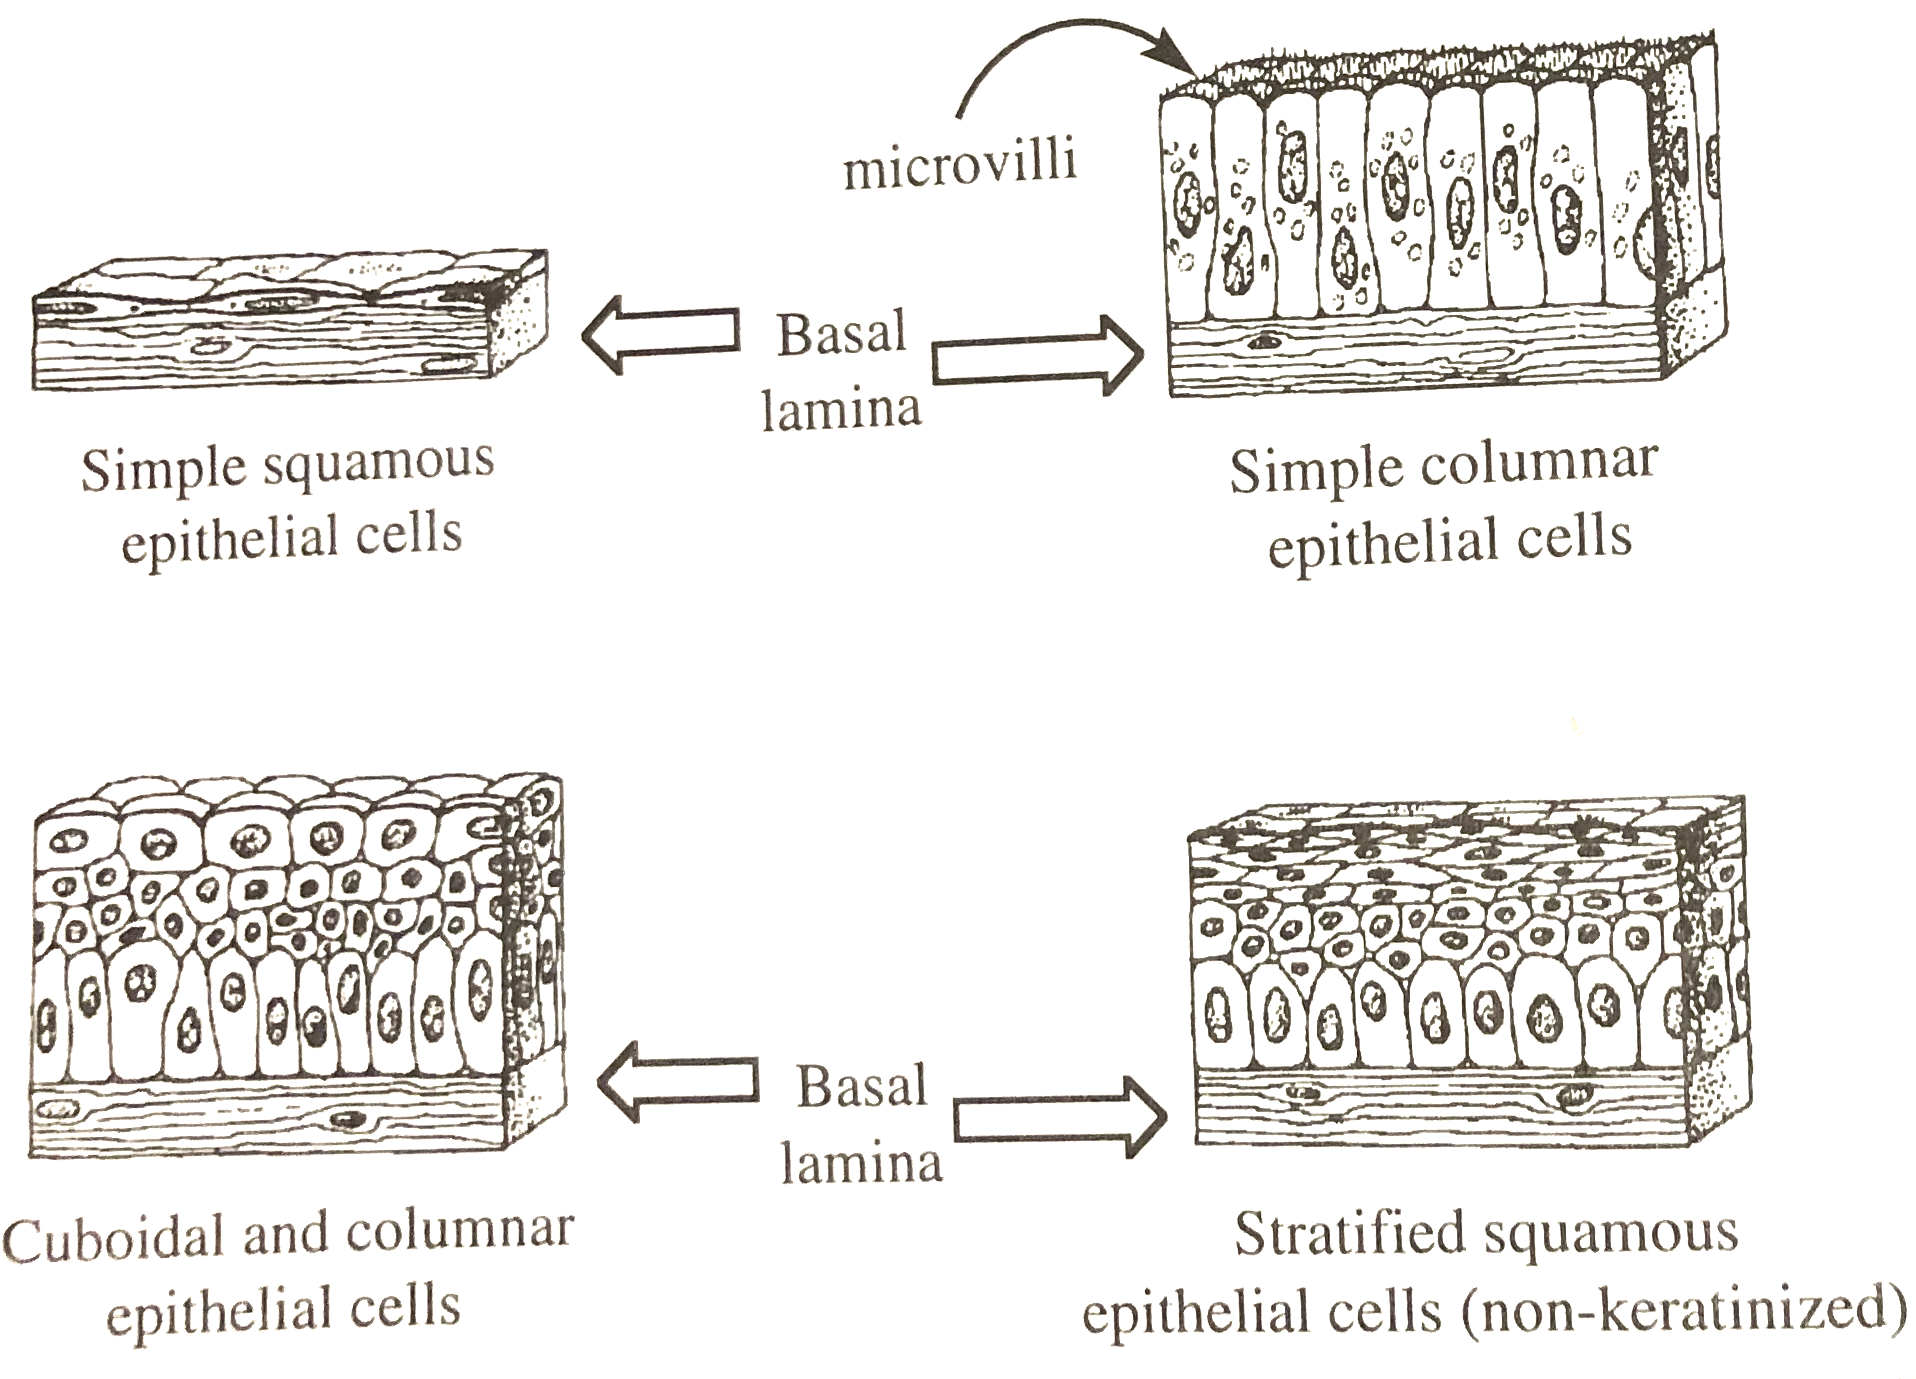
\includegraphics[width=0.7\textwidth]{epithelial.png} \label{epithelial}
\caption{Types of epithelial cells.}
\end{figure}
\indent \textbf{Skin} consists of many layers. The \textbf{epidermal} region contains \textbf{stratified epithelial cells} for protection. Below the epidermis is the \textbf{dermix} with a variety oa structures. Surrounding the hair follicles are \textbf{erector muscles}, which act to straighten the hair shaft. Below the dermis is the \textbf{subcutaneous tissue}. This is where one finds adipose deposits.\\
\indent The inside of the cell is more negatively charged with respect to the outside of the cell. This sets up a voltage that is positive on the outside of the cell. We can calculate the \textbf{membrane voltage} (i.e. potential difference) across the cell's membrane using the \textbf{Nernst equation}:
\begin{equation}
\begin{split}
V_{io}=2.3\frac{RT}{ZF}\log\left(\frac{\left[X\right]_o}{\left[X\right]_i}\right)
\end{split}
\end{equation}
\noindent where $V$ is the voltage in millivolts, $i$ refers to inside, $o$ refers to outside, $Z$ is the ion's valance, and $F$ is Faraday's constant. The inside of a neuron registers a potential difference of about \textbf{-80 mV}. 

\subsection{Action Potentials}
Stimulating a nerve causes the membrane to be \textbf{depolarized}. If the stimulus is strong enough and the depolarization exceeds the \textbf{threshold potential}, then within milliseconds, a burst of \ce{Na+} ions enters and generates an action potential. One millisecond after the burst of \ce{Na+} into the cell, the ion channels that let \ce{Na+} into the cell close and become temporarily inactive\textemdash this is referred to the \textbf{refractory period}, which lasts for several milliseconds. During this time a neuron will not be able to generate another action potential, because the \ce{Na+} channels cannot open to allow the cell membrane to depolarize.\\
\indent Once the \ce{Na+} channels have closed, the \ce{K+} channels begin to open and \ce{K+} begins to leave the cell\textemdash this is referred to as repolarization. The overshoot due to the massive outflux of \ce{K+} ions is called \textbf{hyperpolarization}. The generation of an action potential is said to be an \textbf{all-or-none} phenomenon; an example of a typical action potential is shown in \textbf{Fig. \ref{action_potential}}. \\
\begin{figure}[!ht]
\centering
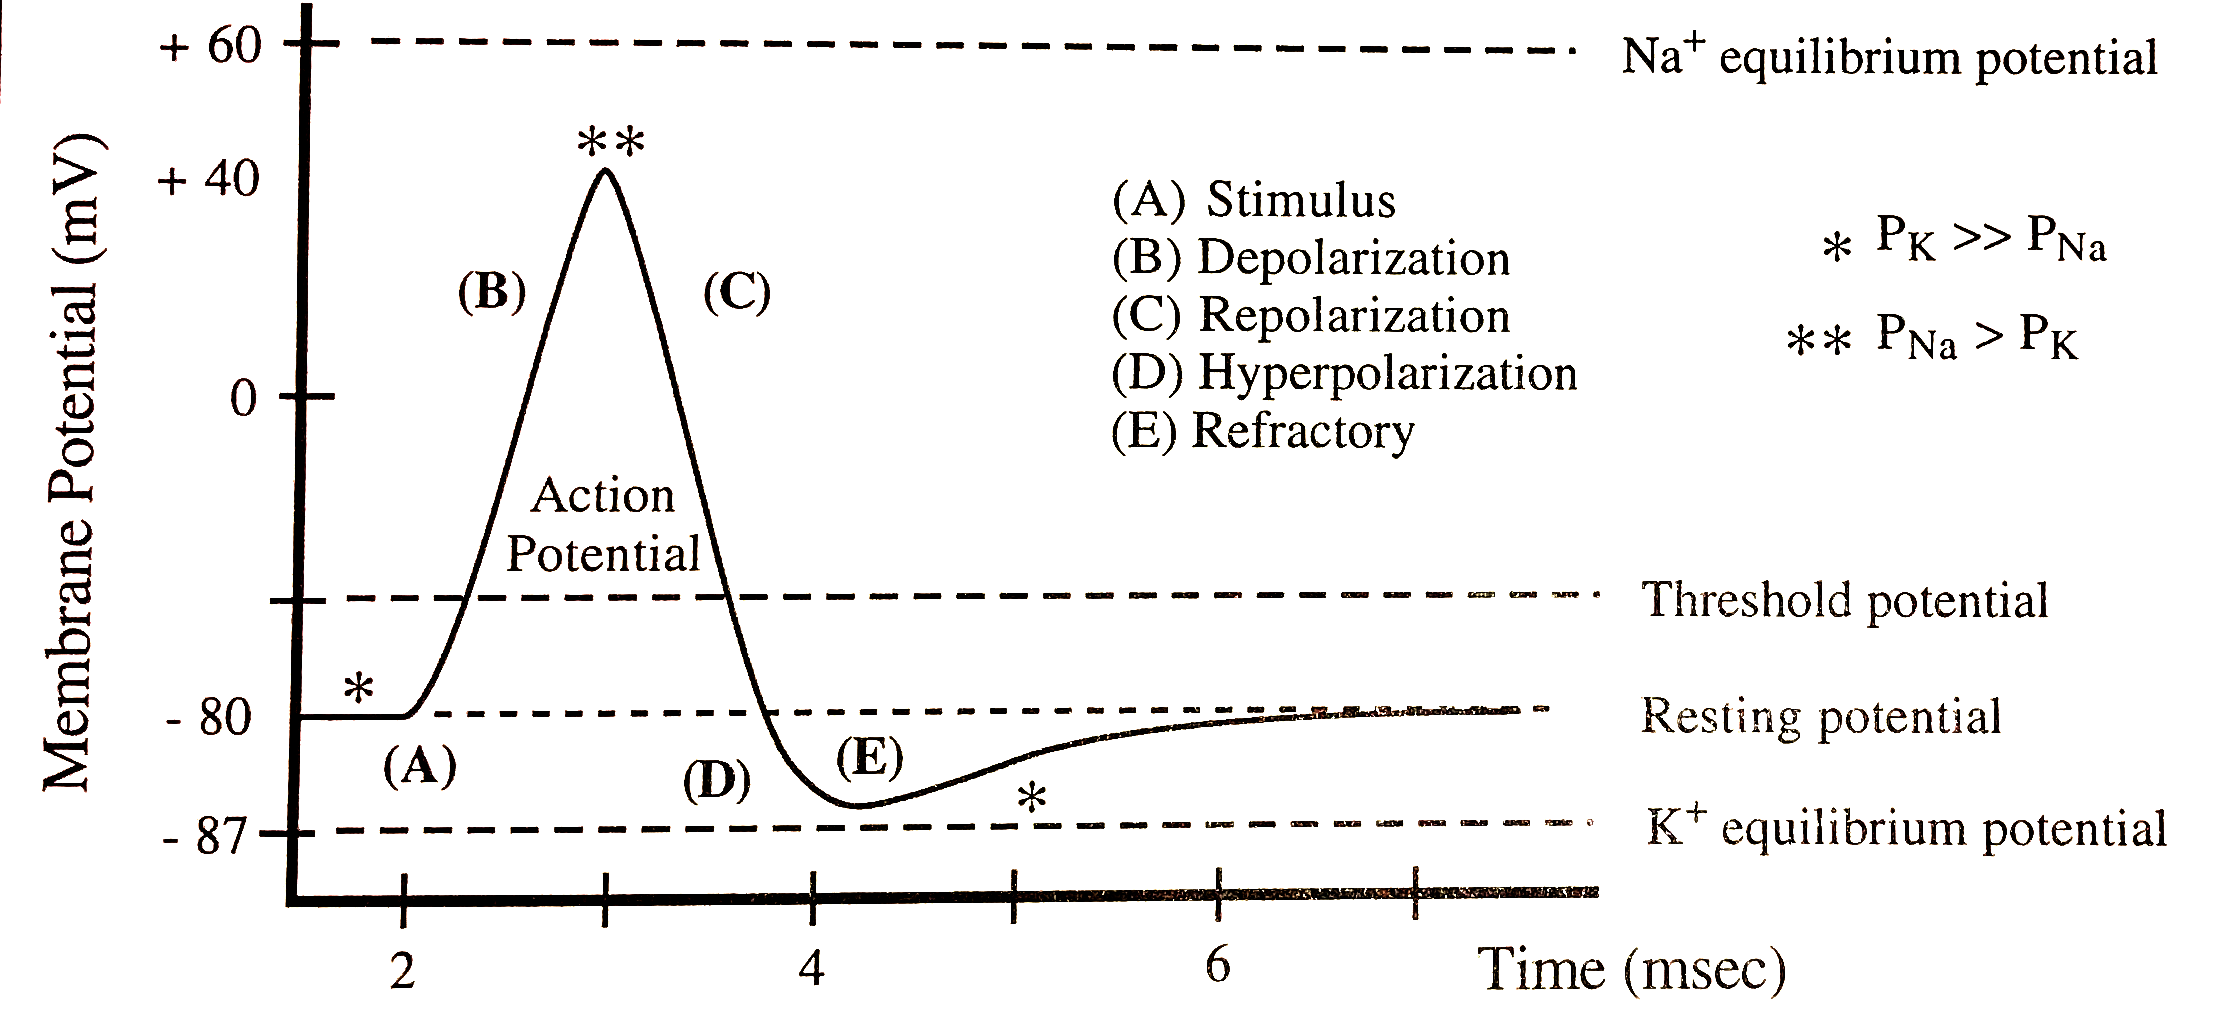
\includegraphics[width=0.7\textwidth]{action_potential.png} \label{action_potential}
\caption{A typical action potential. $P_K$ is the cell's permeability to \ce{K+} and $P_{Na}$ is the cell's permeability to \ce{Na+}.}
\end{figure}
\indent Larger diameter neurons will conduct an action potential further and faster than a small diameter neuron. This means that the ability of a neuron to conduct a current depends on the cross-sectional area of that neuron. \\
\indent \textbf{Myelinated} nerves have the ability to greatly increase the rate at which action potentials are conducted. This is because myelin acts as an electrical insulator and prevents the transfer of ions across the plasma membrane of the axon. This allows the nerve impulse to `jump' from node to node along the axon, referred to as \textbf{saltatory conduction}. \textbf{Glial cells} attach themselves to a section of an unmyelinated axon and begin to rotate around that axon to deposit a myelin sheath. The deposition of myelin along the axon is interrupted by areas where there is no myelin, called the \textbf{nodes of Ranvier}. Glial cells in the central nervous system (CNS) are called \textbf{oligodendrocytes}, while glial cells in the peripheral nervous system (PNS) are called \textbf{Schwann cells}. The CNS is made up of the brain and spinal cord while the \textbf{peripheral nervous system} represents the nerves in the periphery. 

\subsection{The Neuromuscular Junction}
At the end of the axon is a specialized area called the \textbf{terminal bouton}. Neuromuscular junctions involve a terminal bouton with hundreds of thousands of \textbf{synaptic vesicles} that contain the excitatory neurotransmitter \textbf{acetylcholine (ACh)}, which is synthesized in the cytosol of the neuron from the molecules \textbf{acetyl-CoA} and \textbf{choline}. As the action potential reaches the terminal bouton, it triggers the opening of \ce{Ca^2+} channels that generate a transient influx of \ce{Ca^2+} into the terminal region, which causes synaptic vesicles to fuse with the presynaptic membrane and release ACh into the synaptic cleft via exocytosis. \ce{Ca^2+} is pumped out of the cytosol and back into the extracellular fluid. ACh then binds to specific postsynaptic membrane receptors, which conformationally changes the ionphore channel receptor so that it can let ions like \ce{Na+} through. As \ce{Na+} enters the postsynaptic membrane, the muscle fiber begins to depolarize and an action potential is eventually generated. A diagram of the neuromuscular junction is shown in \textbf{Fig. \ref{neuromuscular}}. \\
\begin{figure}[!ht]
\centering
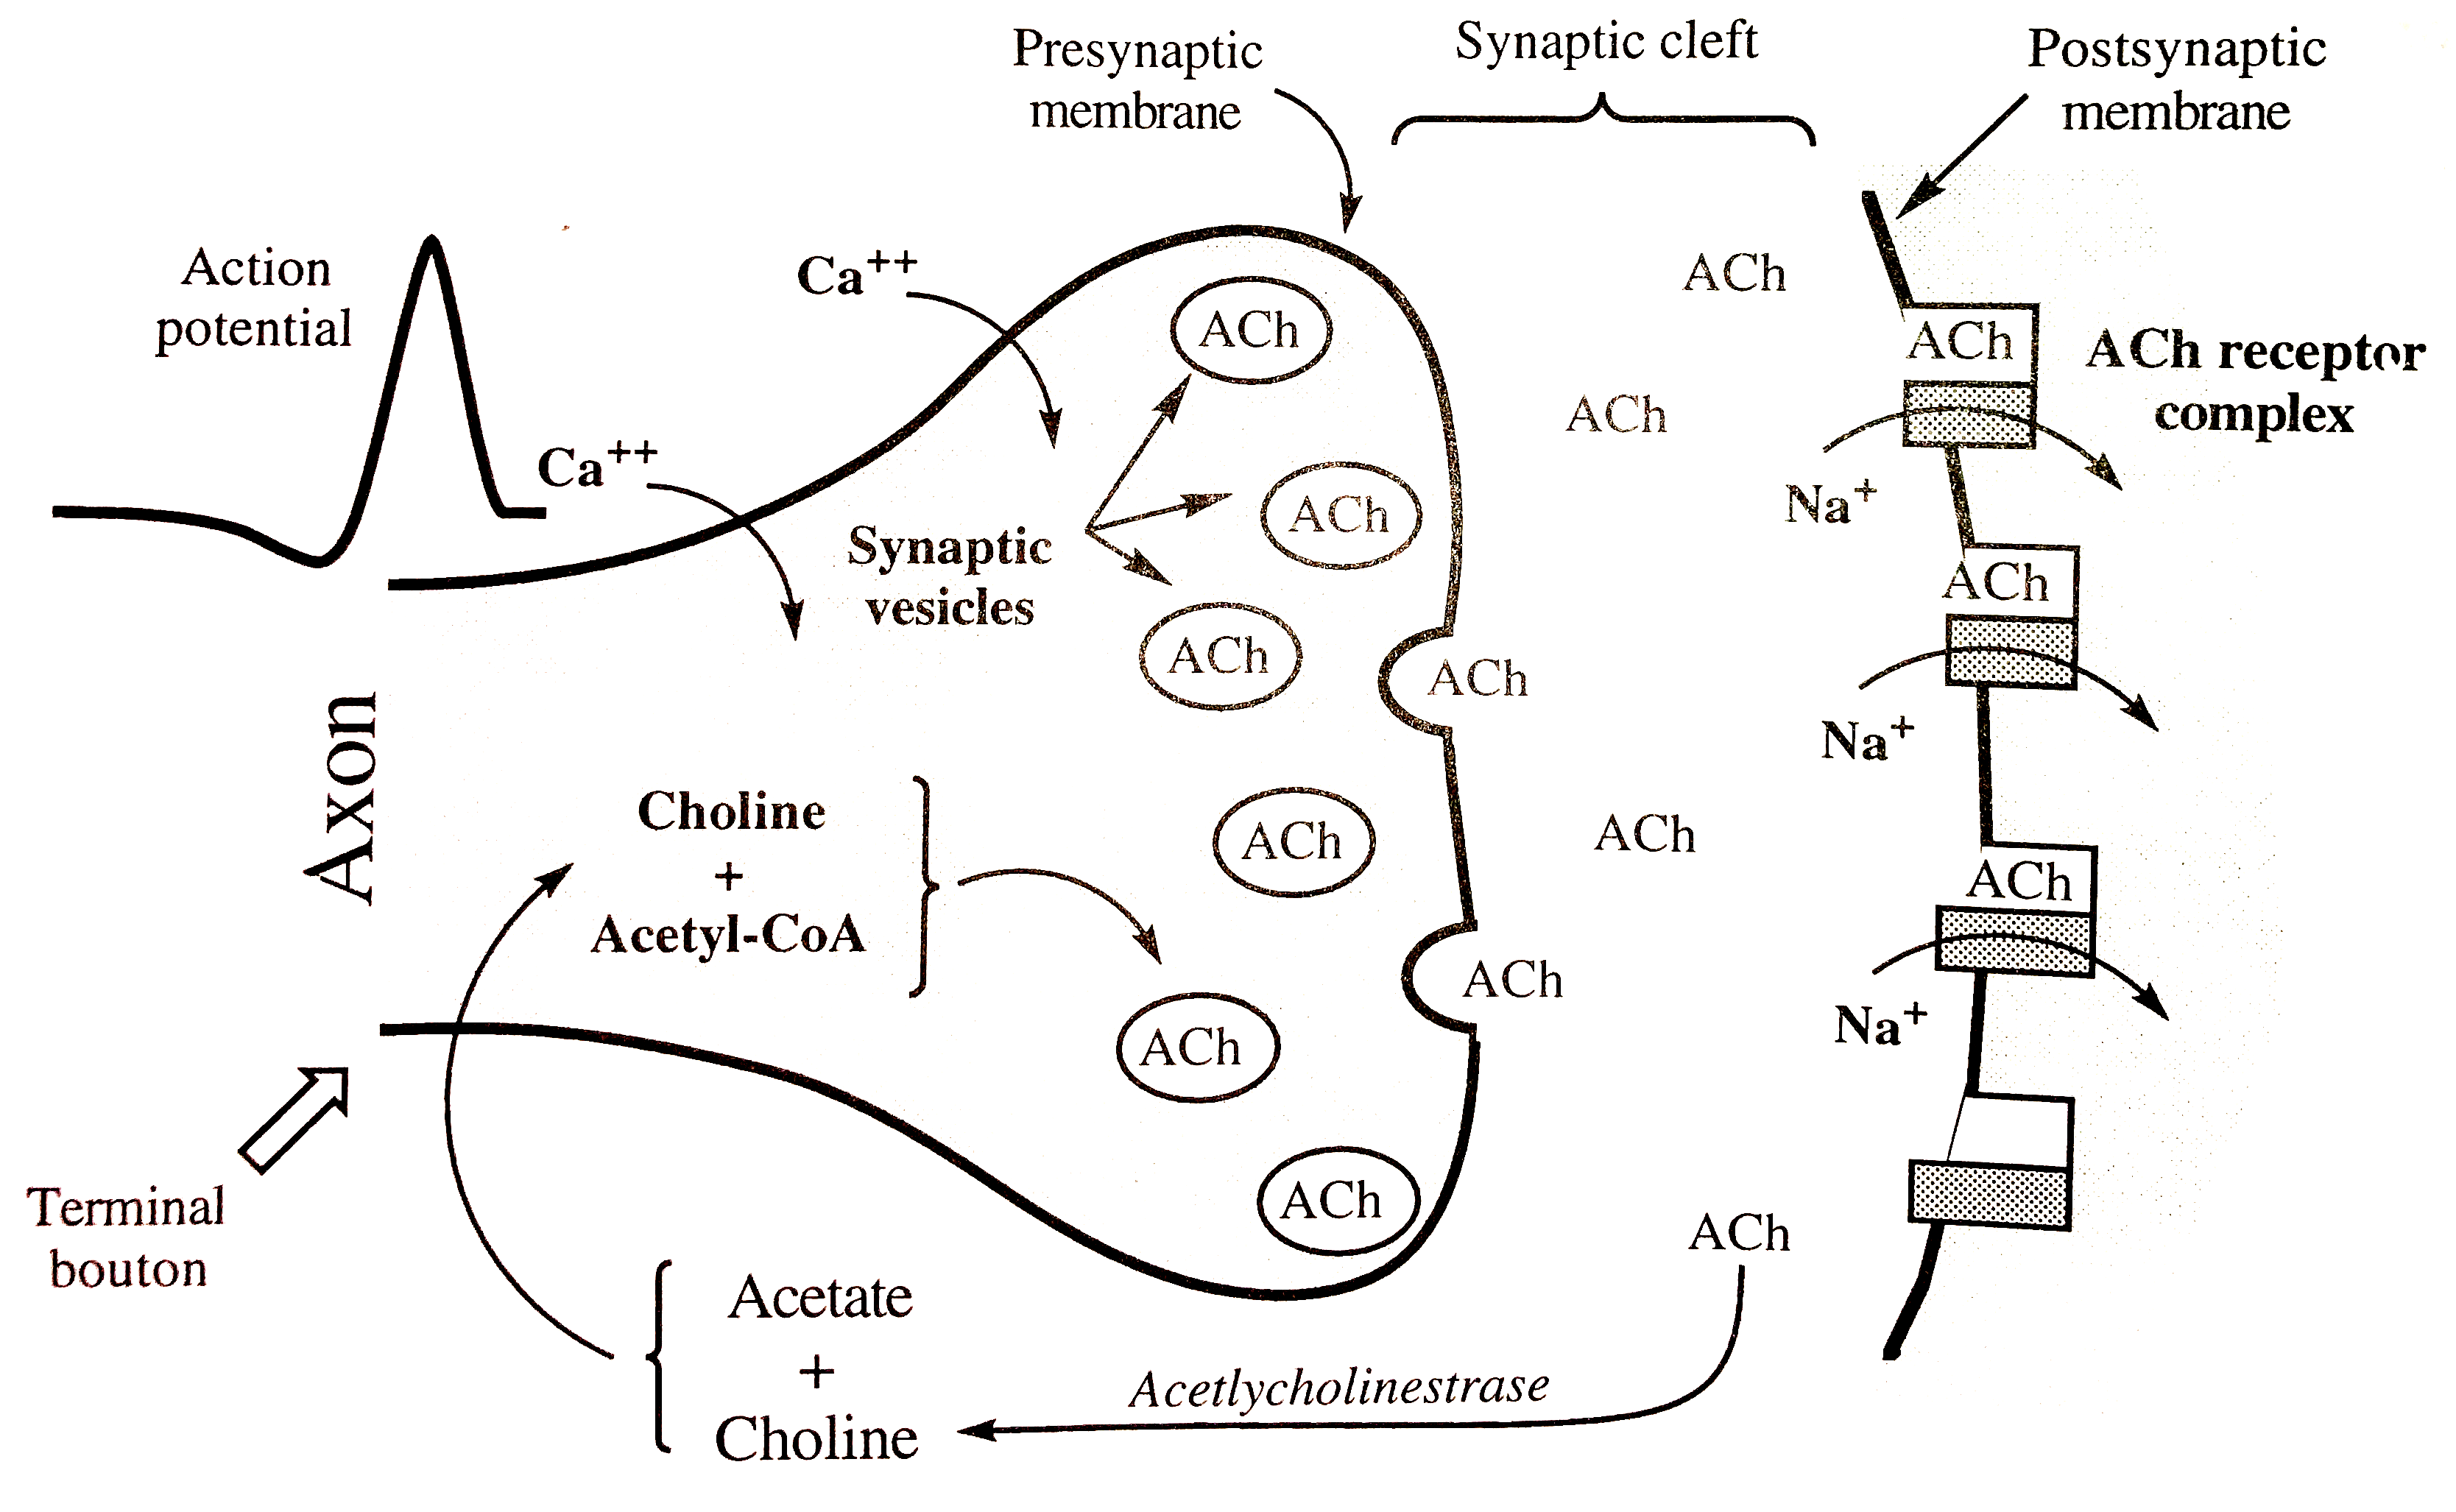
\includegraphics[width=0.7\textwidth]{neuromuscular.png} \label{neuromuscular}
\caption{Presynaptic and postsynaptic membranes of a neuromuscular junction.}
\end{figure}
\indent If ACh were to remain in the synaptic cleft, then it would continue to bind to the postsynaptic membrane and action potentials would continually be generated. This could result in prolonged muscle spasms. However, the enzyme \textbf{\textit{acetylcholinesterase}}, which is bound to the surface of the postsynaptic membrane, hydrolyzes ACh to acetate and choline. Other neurotransmitters include the amino acid \textbf{glutamate} and the amino acid derivatives \textbf{epinephrine}, \textbf{norepinephrine}, \textbf{dopamine}, and \textbf{serotonin}. \\
\indent ACh binding to its postsynaptic membrane receptor is referred to as an \textbf{excitatory} postsynaptic potential (\textbf{EPSP}s), since it elicits an excitatory response that generates an action potential. There can also be \textbf{inhibitory} postsynaptic potentials (\textbf{IPSP}s). EPSPs cause an increase in the membrane permeability to \ce{Na+} ions, while IPSPs cause an increase in the permeability of the postsynaptic membrane to \ce{K+} and \ce{Cl-} ions. \\
\indent When two action potentials are coming toward each other in the same neuron, both action potentials will be stopped when they meet. This is because the region in front of each action potential is continuously being depolarized, while the region behind the action potential is in its refractory period for a few milliseconds and cannot immediately be depolarized by the other action potential. 

\subsection{The Sarcomere} 
Muscles are multinucleated. They don't divide, but just get larger (i.e. with exercise). Skeletal muscles have \textbf{striations} in both the transverse and longitudinal directions. The striations in the longitudinal direction are due to \textbf{myofibrils}, which contain the contractile units of the muscle. Each contractile unit, bounded by a structure referred to as the \textbf{Z-line}, is referred to as a \textbf{sarcomere} and each sarcomere contains two types of contractile proteins. The thin contractile protein is called \textbf{actin} and the thick contractile protein is called \textbf{myosin}. The myosin thick filament comprises the \textbf{A-band}, and the region between two A-bands is the \textbf{I-band}. The \textbf{H-zone} is that region in the center of the A-band and between the ends of the actin filaments. All these components of the sarcomere are shown in \textbf{Fig. \ref{sarcomere}}.\\
\begin{figure}[!ht]
\centering
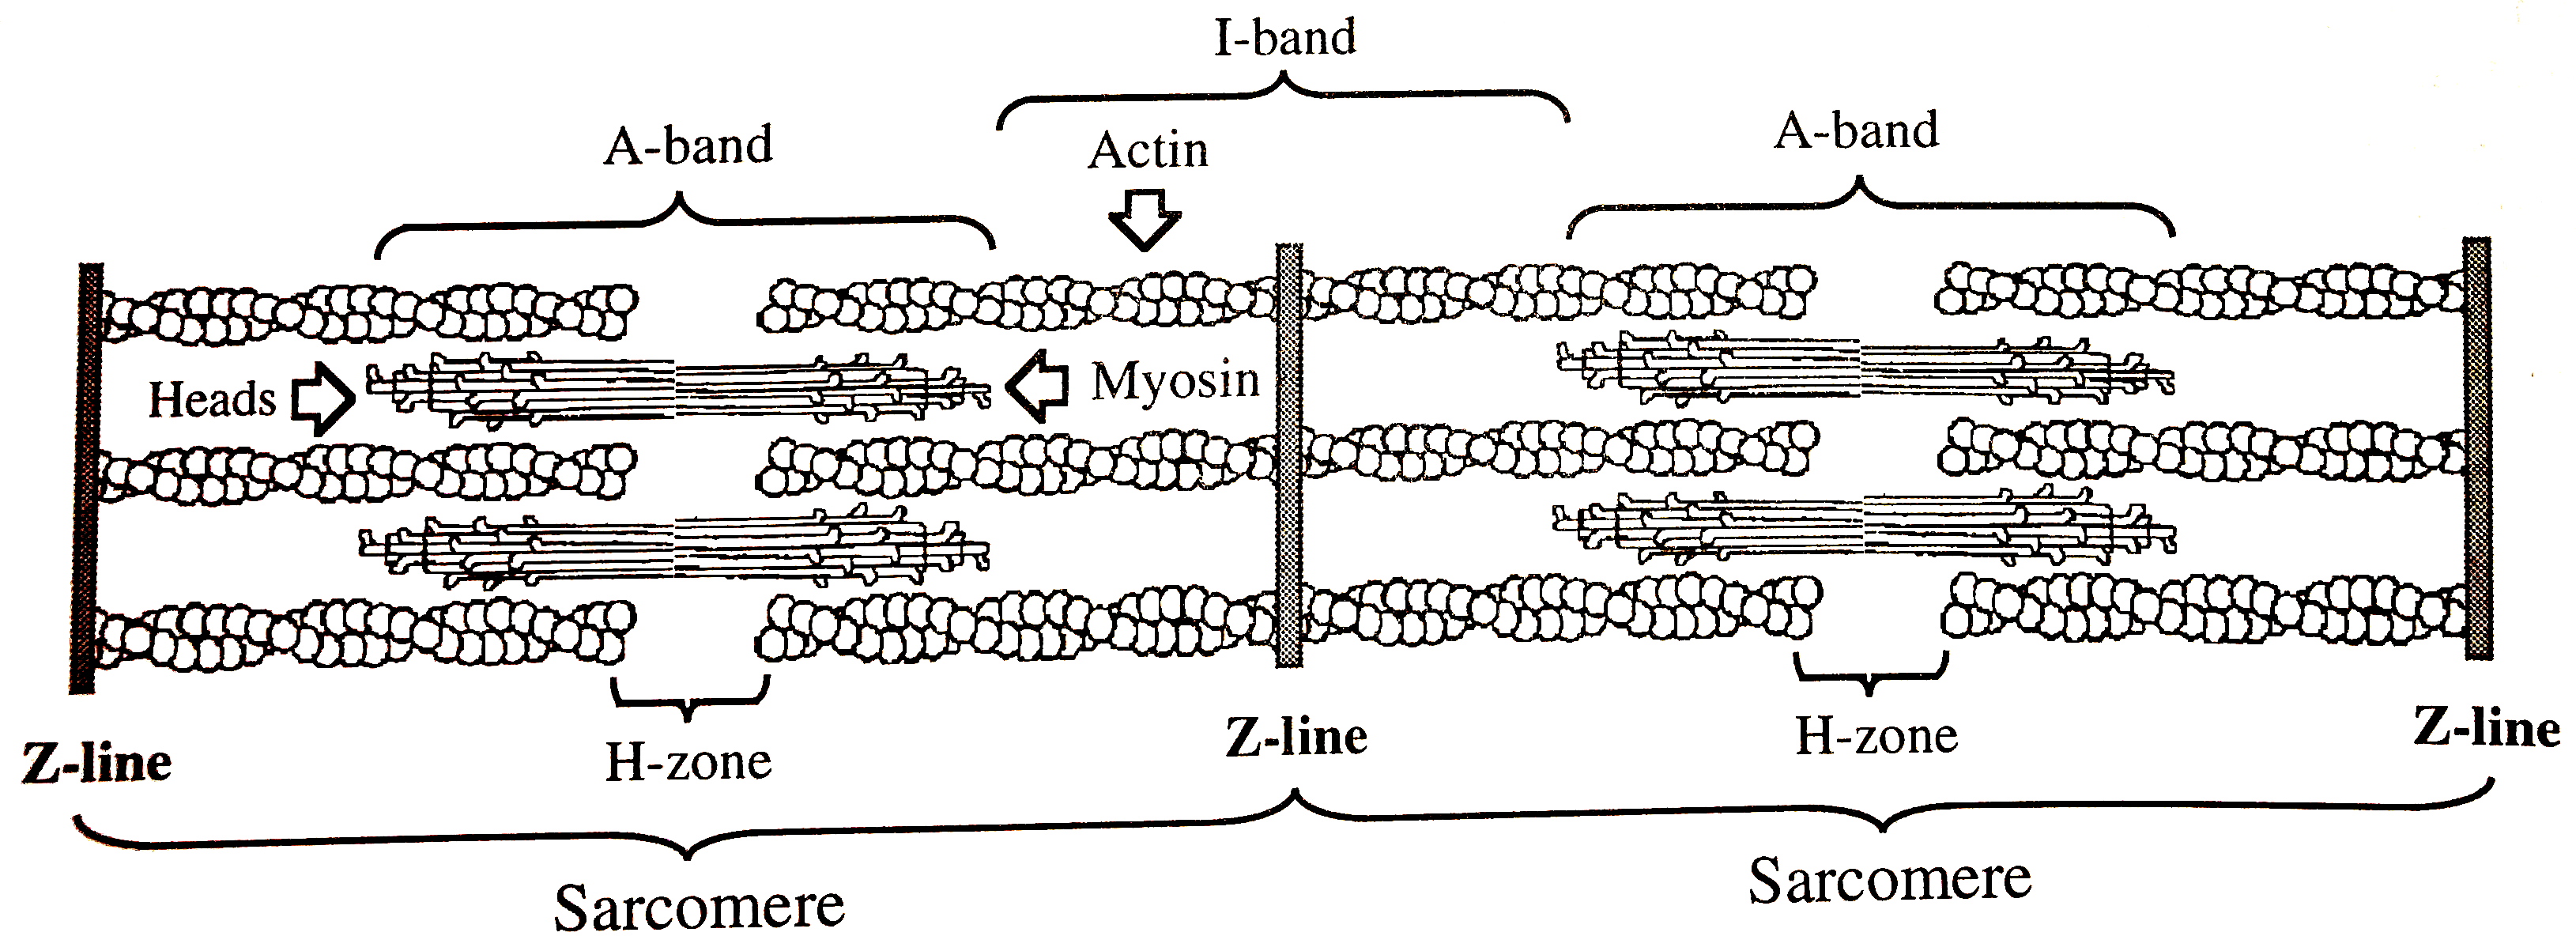
\includegraphics[width=0.7\textwidth]{sarcomere.png} \label{sarcomere}
\caption{Sarcomere details.}
\end{figure}
\indent Let's consider the interaction between actin and myosin. When a muscle is in its relaxed state, ATP is bound to the myosin head groups. The myosin head is not bound to the actin filament, because ATP reduces myosin's affinity for actin. The ATP can be hydrolyzed to ADP, and the myosin head now undergoes a corresponding conformational change that is higher in energy and stable. The myosin-ADP-\ce{P_i} (\ce{P_i} is the inorganic phosphate hydrolysis product) head complex binds to the actin filament. This step is dependent on \ce{Ca^2+} being present. The interaction between the actin filaments and myosin head groups releases the ADP and \ce{P_i} from the myosin heads, causing a conformational change in the myosin heads. This step is called the \textbf{power stroke}, and the product of this step is referred to as the \textbf{rigor complex} or \textbf{rigor state}. In order for the myosin heads to dissociate from actin filaments, ATP needs to bind to those myosin heads. This contraction cycle of muscles is shown in \textbf{Fig. \ref{contraction_cycle}}.\\
\begin{figure}[!ht]
\centering
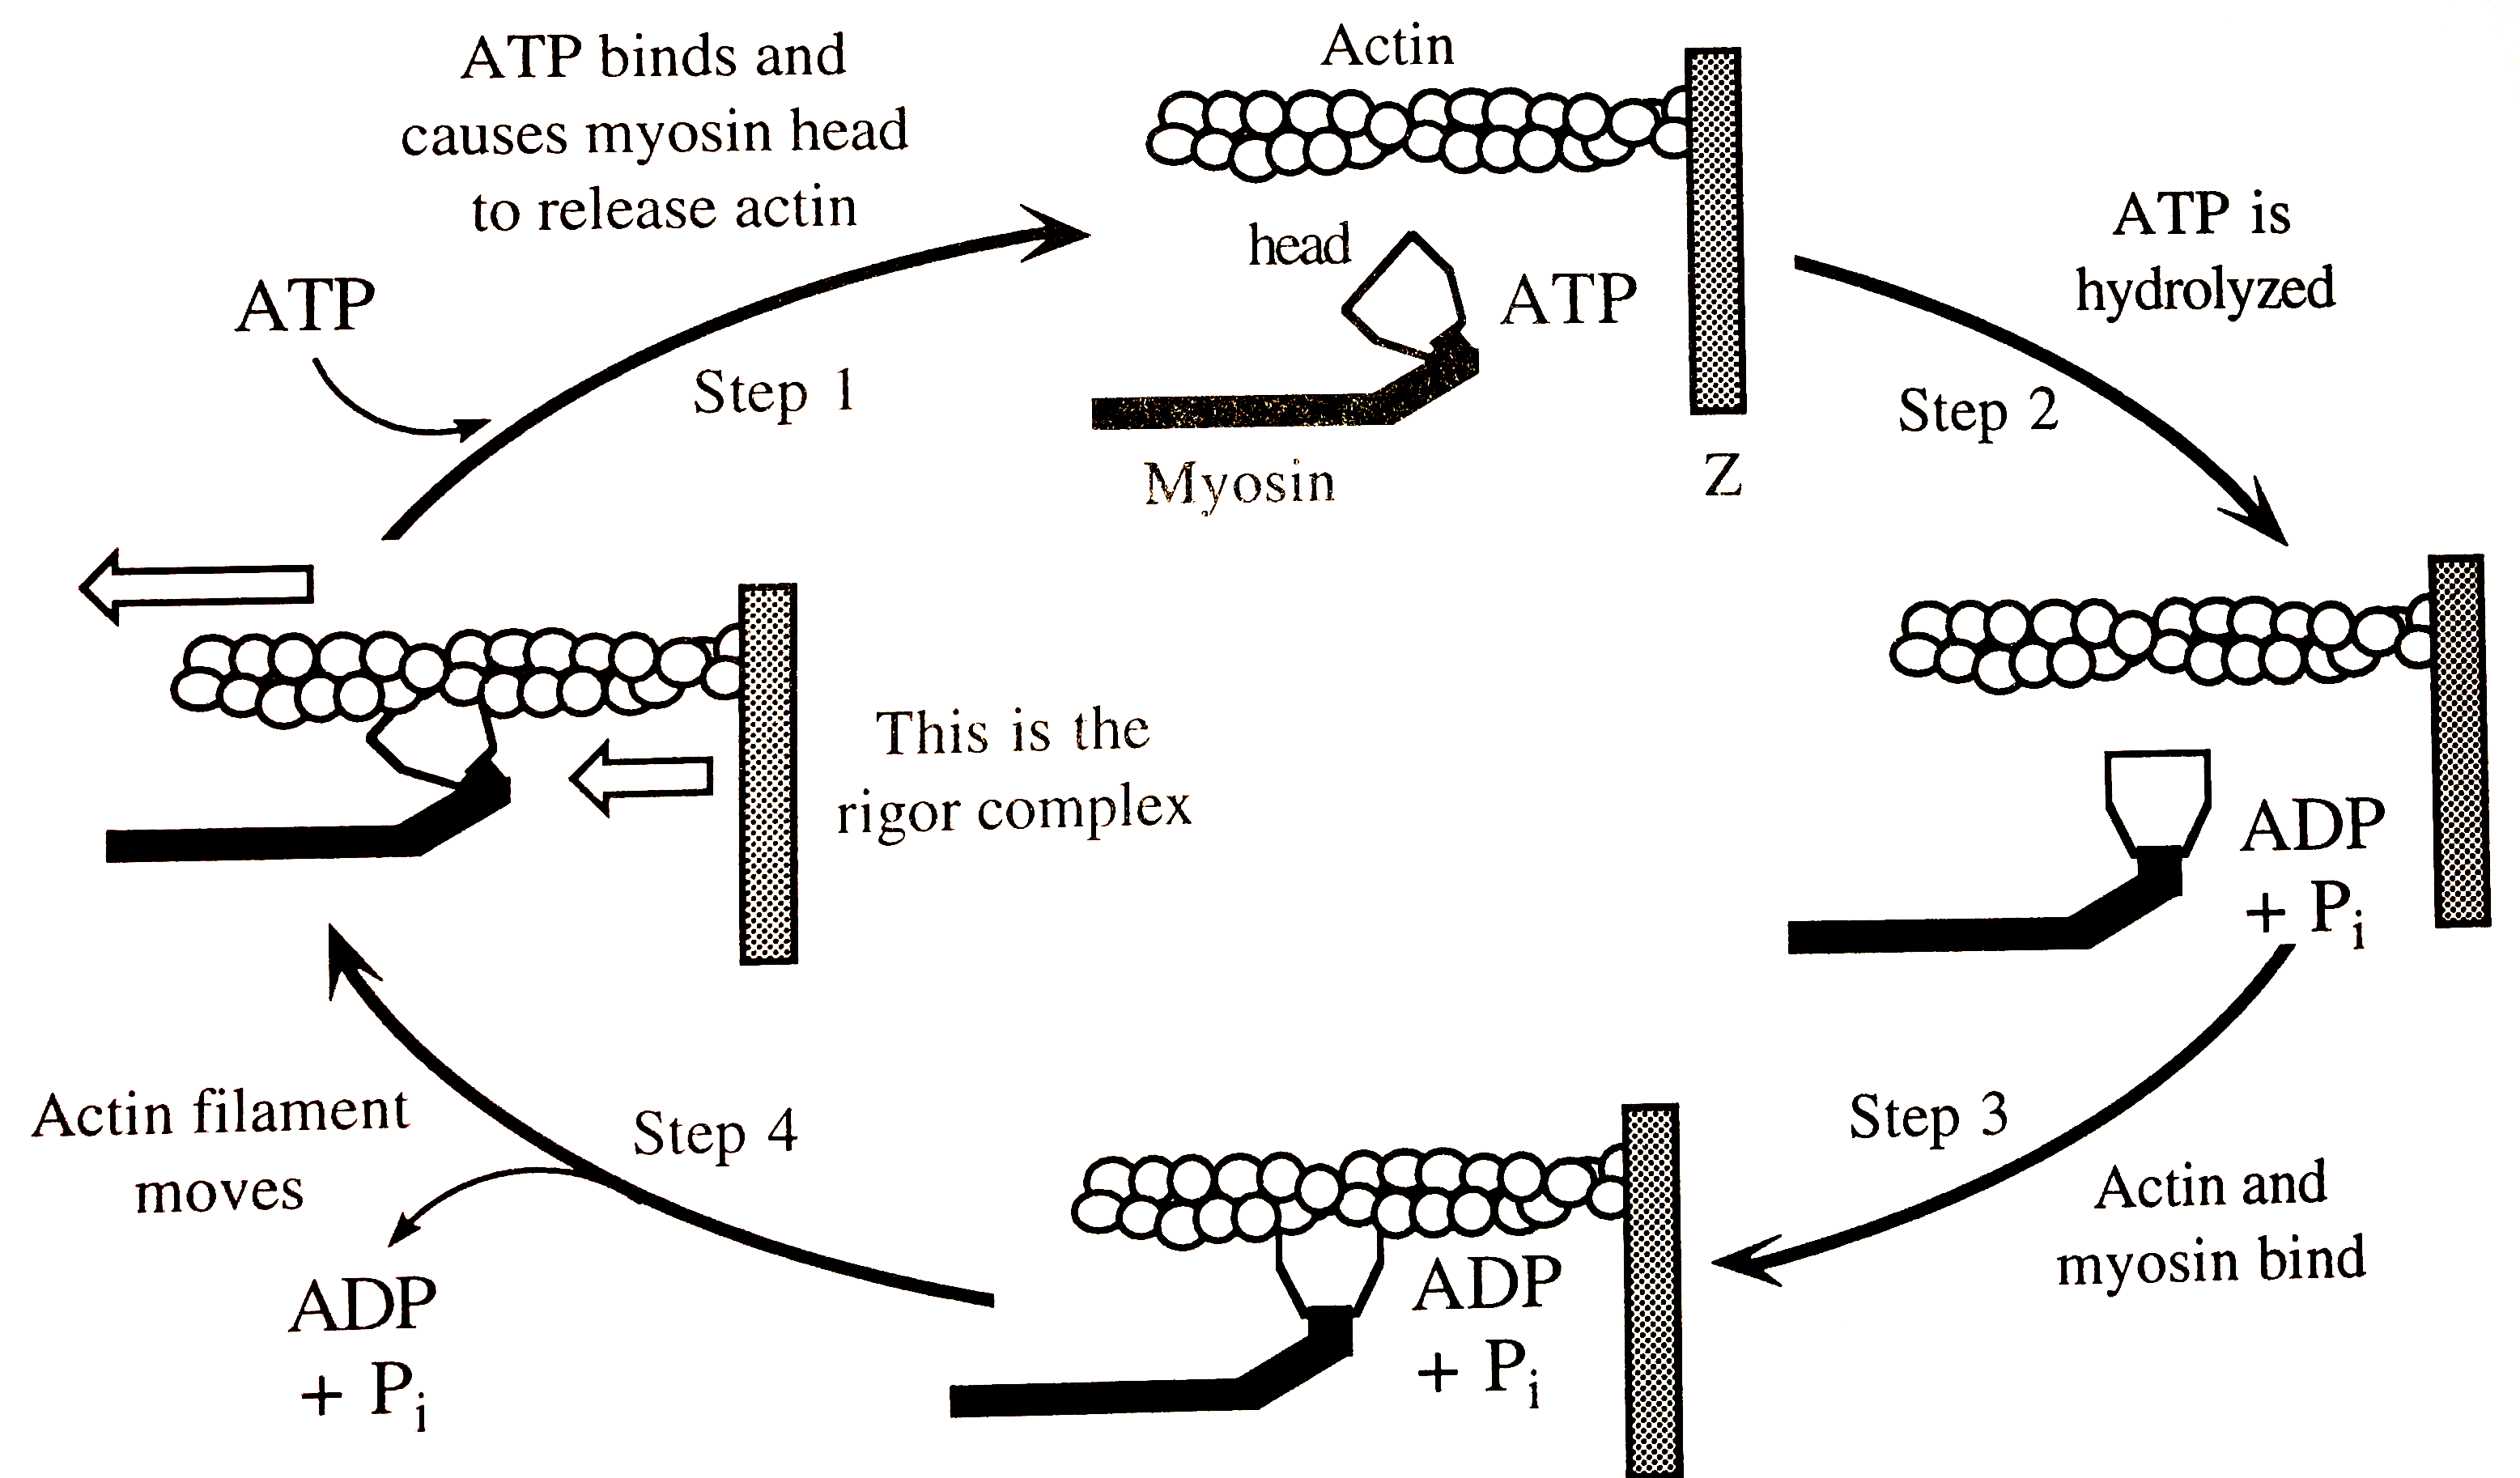
\includegraphics[width=0.7\textwidth]{contraction_cycle.png} \label{contraction_cycle}
\caption{The contraction cycle of actin and myosin.}
\end{figure}
\indent \textbf{Tropomyosin} is a protein that runs the length of the grooves of actin's helical structure. When tropomyosin resides in the actin groove, it covers up the binding sites for the myosin heads and prevents those head groups from attaching to the actin filament. \textbf{Troponin} is a binding protein that interacts with tropomyosin, actin, and \ce{Ca^2+}. When \ce{Ca^2+} is bound to a particular subunit of the troponin complex, it causes tropomyosin to shift its position and expose the myosin head binding sites. Myosin then can bind to the actin filaments, and muscle contraction follows. If \ce{Ca^2+} is not present, then no myosin binding is possible and the muscle is in the \textbf{relaxed state}. This interaction is shown in \textbf{Fig. \ref{troponin}}.\\
\begin{figure}[!ht]
\centering
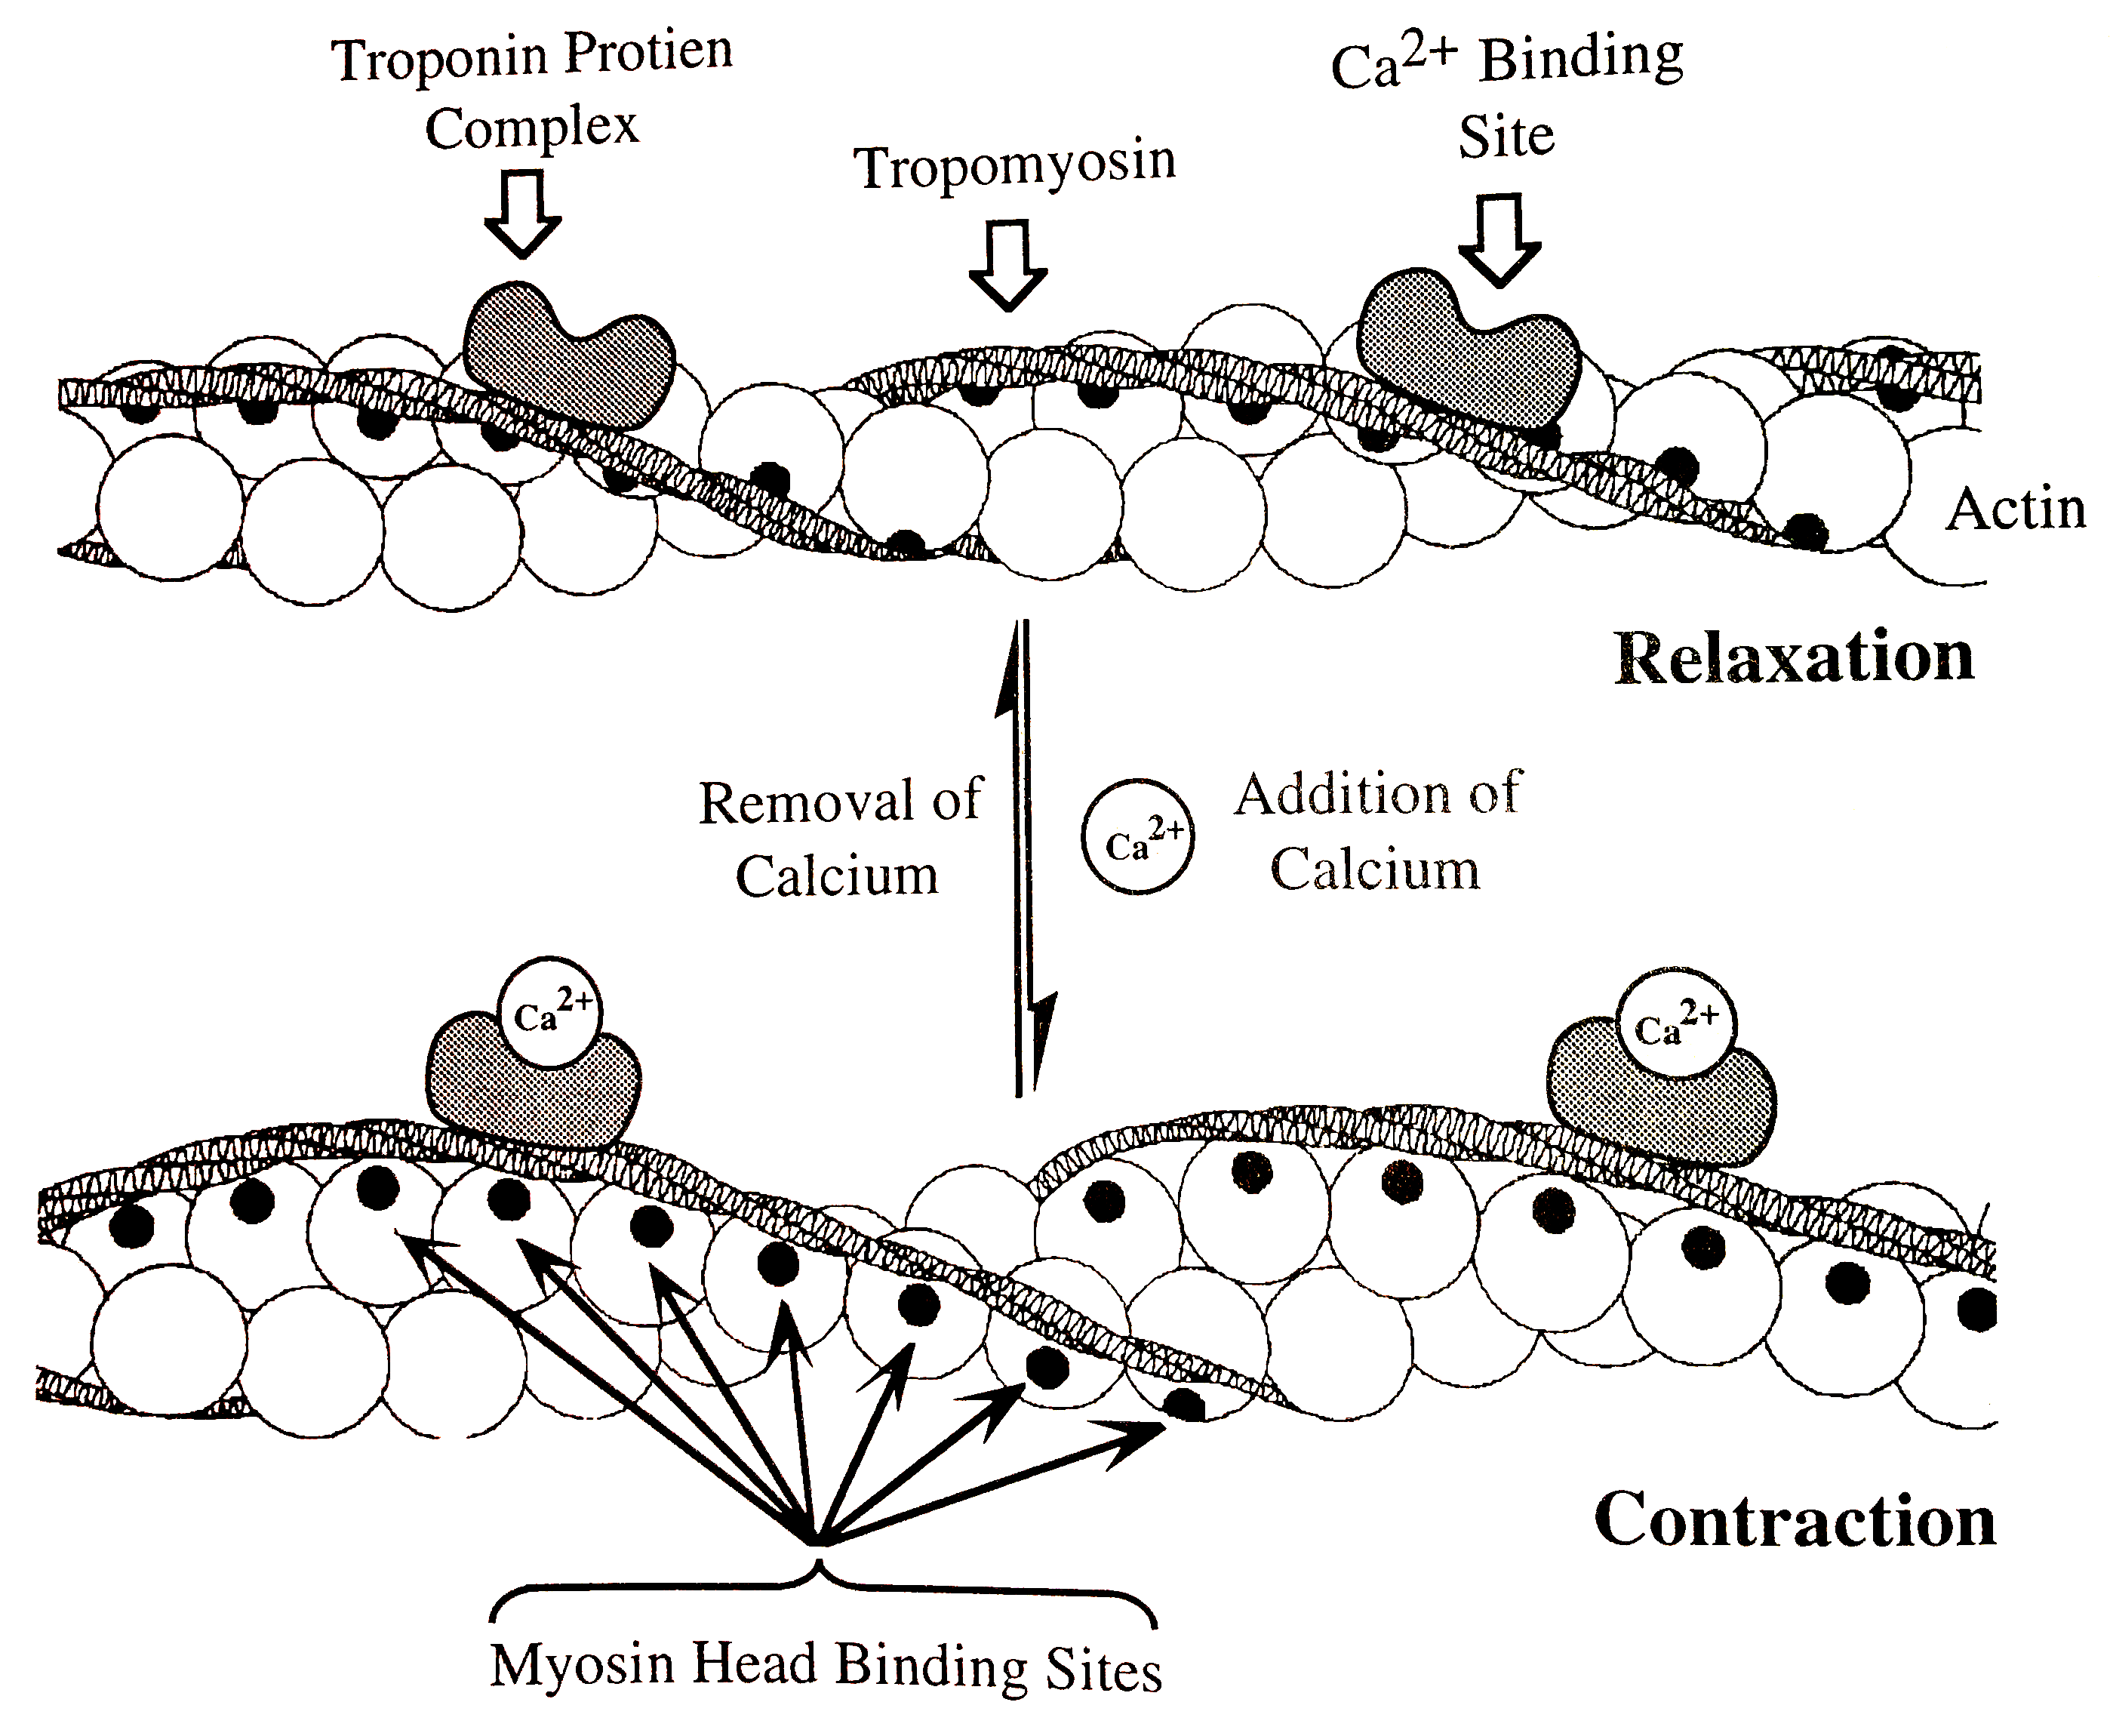
\includegraphics[width=0.7\textwidth]{troponin.png} \label{troponin}
\caption{The interaction between troponin, tropomyosin, and calcium in the sarcomere.}
\end{figure}
\indent \textbf{Myofibrils} are the basic, rod-like units of a muscle cell. Surrounding each myofibril is a membranous structure called the \textbf{sarcoplasmic reticulum}, a modified version of the endoplasmic reticulum. \ce{Ca^2+} is sequestered within this smooth membranous structure. Also surrounding each myofibril is an invagination of the sarcolemma (i.e. the plasma membrane) called the \textbf{T-tubule}. Action potentials pass down each T-tubule and stimulate the release of \ce{Ca^2+} from the sarcoplasmic reticulum. \ce{Ca^2+} then bind to the troponin complex, allowing for synchronized muscle contraction. Once contraction has taken place and the nerve impulse has ceased, the \ce{Ca^2+} in the cytosol is pumped back into the sarcoplasmic reticulum by a \ce{Ca^2+}-ATPase pump.\\
\indent The strength of muscle contraction can be varied by (1) the size of the motor unit, which is simply a motor neuron and the muscle fibers that it innervates, (2) the number of available motor units, and (3) the amount of actin and myosin contained within each cell. Smaller motor units means greater precision and lower strength. Less motor units means lower strength.
\begin{figure}[!ht]
\centering
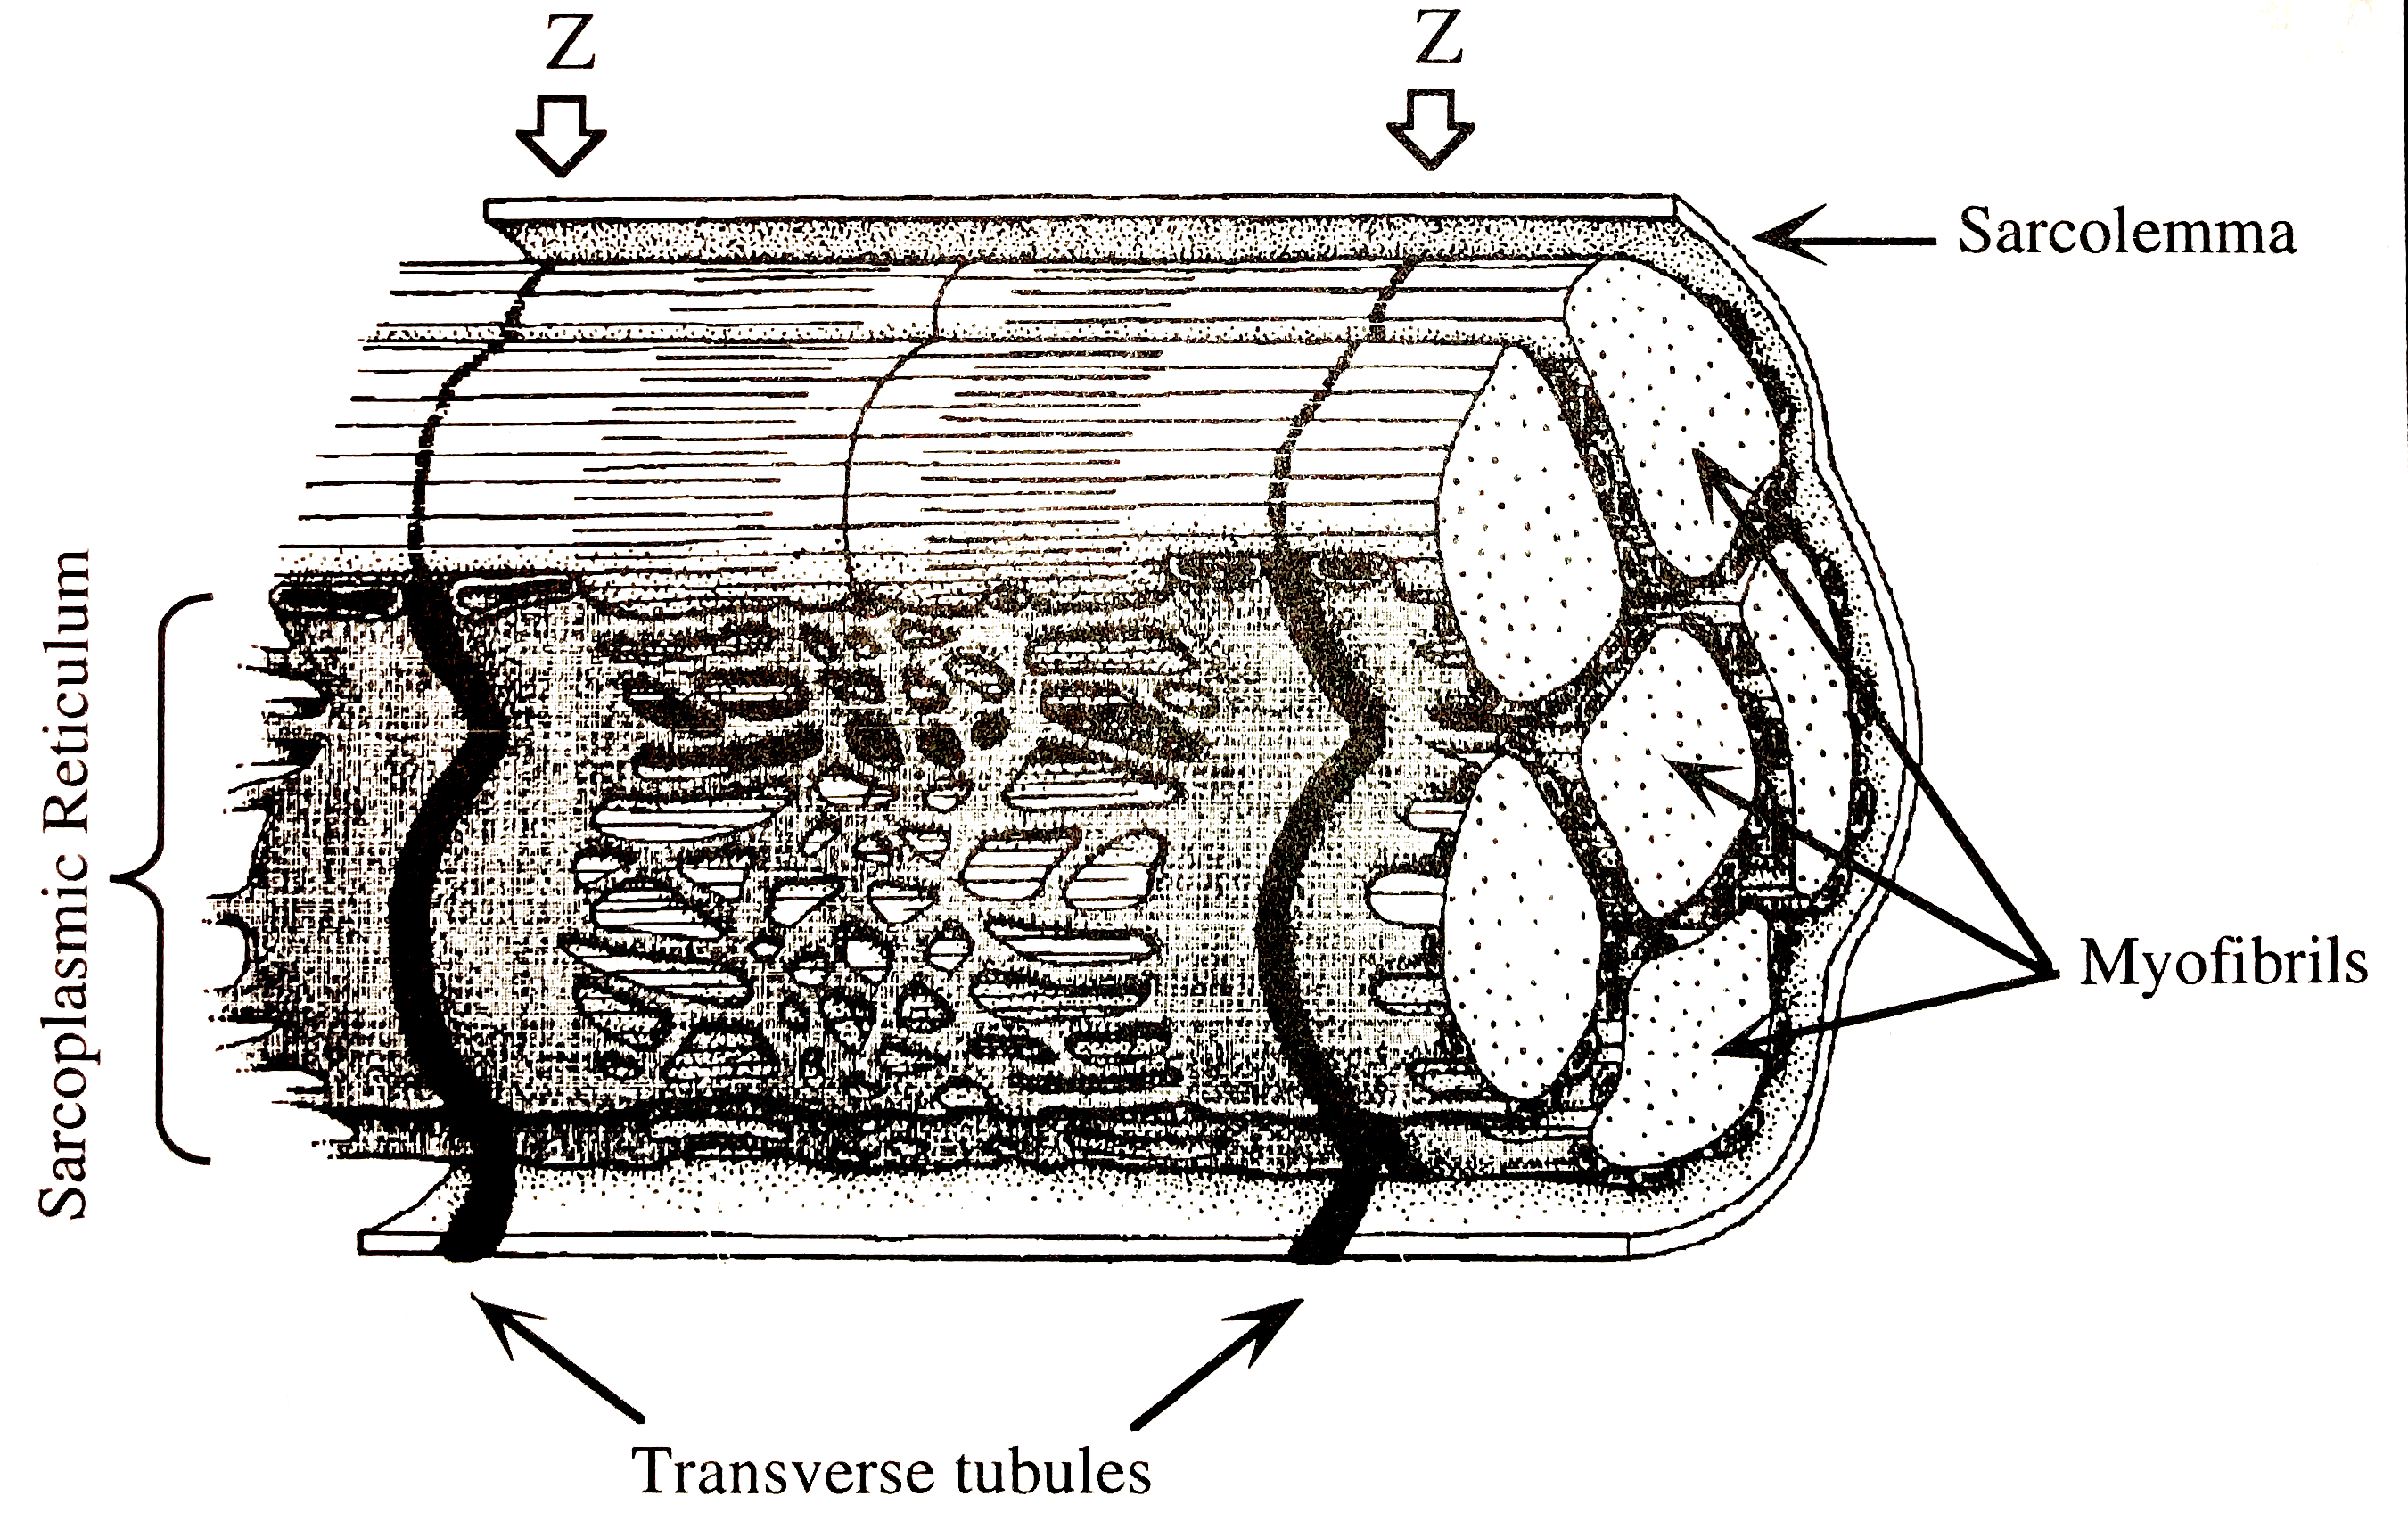
\includegraphics[width=0.7\textwidth]{sarcoplasmic_reticulum.png} \label{sarcoplasmic_reticulum}
\caption{The sarcoplasmic reticulum.}
\end{figure}

\subsection{Nervous System Components}
A grouping of nerve cells is called a \textbf{ganglion}. The three basic anatomical division of the vertebrate brain are the \textit{forebrain} (prosencephalon), \textit{midbrain} (mesencephalon), and \textit{hindbrain} (rhombencephalon). Inferior to the brain is the spinal cord, from which the nerves extend into the limbs and extremities. If a neuron carries information \textit{into} the spinal cord and brain, that neuron is said to be an \textbf{afferent (sensory) neuron}. If a neuron carries the information away from the CNS, that neuron is said to be an \textbf{efferent (motor) neuron}. \\
\indent The \textbf{prosencephalon} includes the \textbf{cerebrum}, \textbf{thalamus}, and \textbf{hypothalamus}. The cerebrum is divided into the right and left cerebral hemispheres, joined by the \textbf{corpus callosum}. The cerebral hemispheres are divided into the \textbf{frontal lobes} (associated with movement and personality), \textbf{parietal lobes} (associated with touch and stretch sensation), \textbf{occipital lobes} (associated with vision), and \textbf{temporal lobes} (associated with hearing). The outermost layer of the cerebrum is called the \textbf{cerebral cortex}, consisting of \textbf{gray matter} (nerve cell bodies and their dendrites) and \textbf{white matter} (myelinated axons of the nerve cells). In the spinal cord, the gray matter is more centralized, while the white matter is more peripheral. The anatomical divisions of the vertebrate brain are shown in \textbf{Fig. \ref{brain}}.\\
\begin{figure}[!ht]
\centering
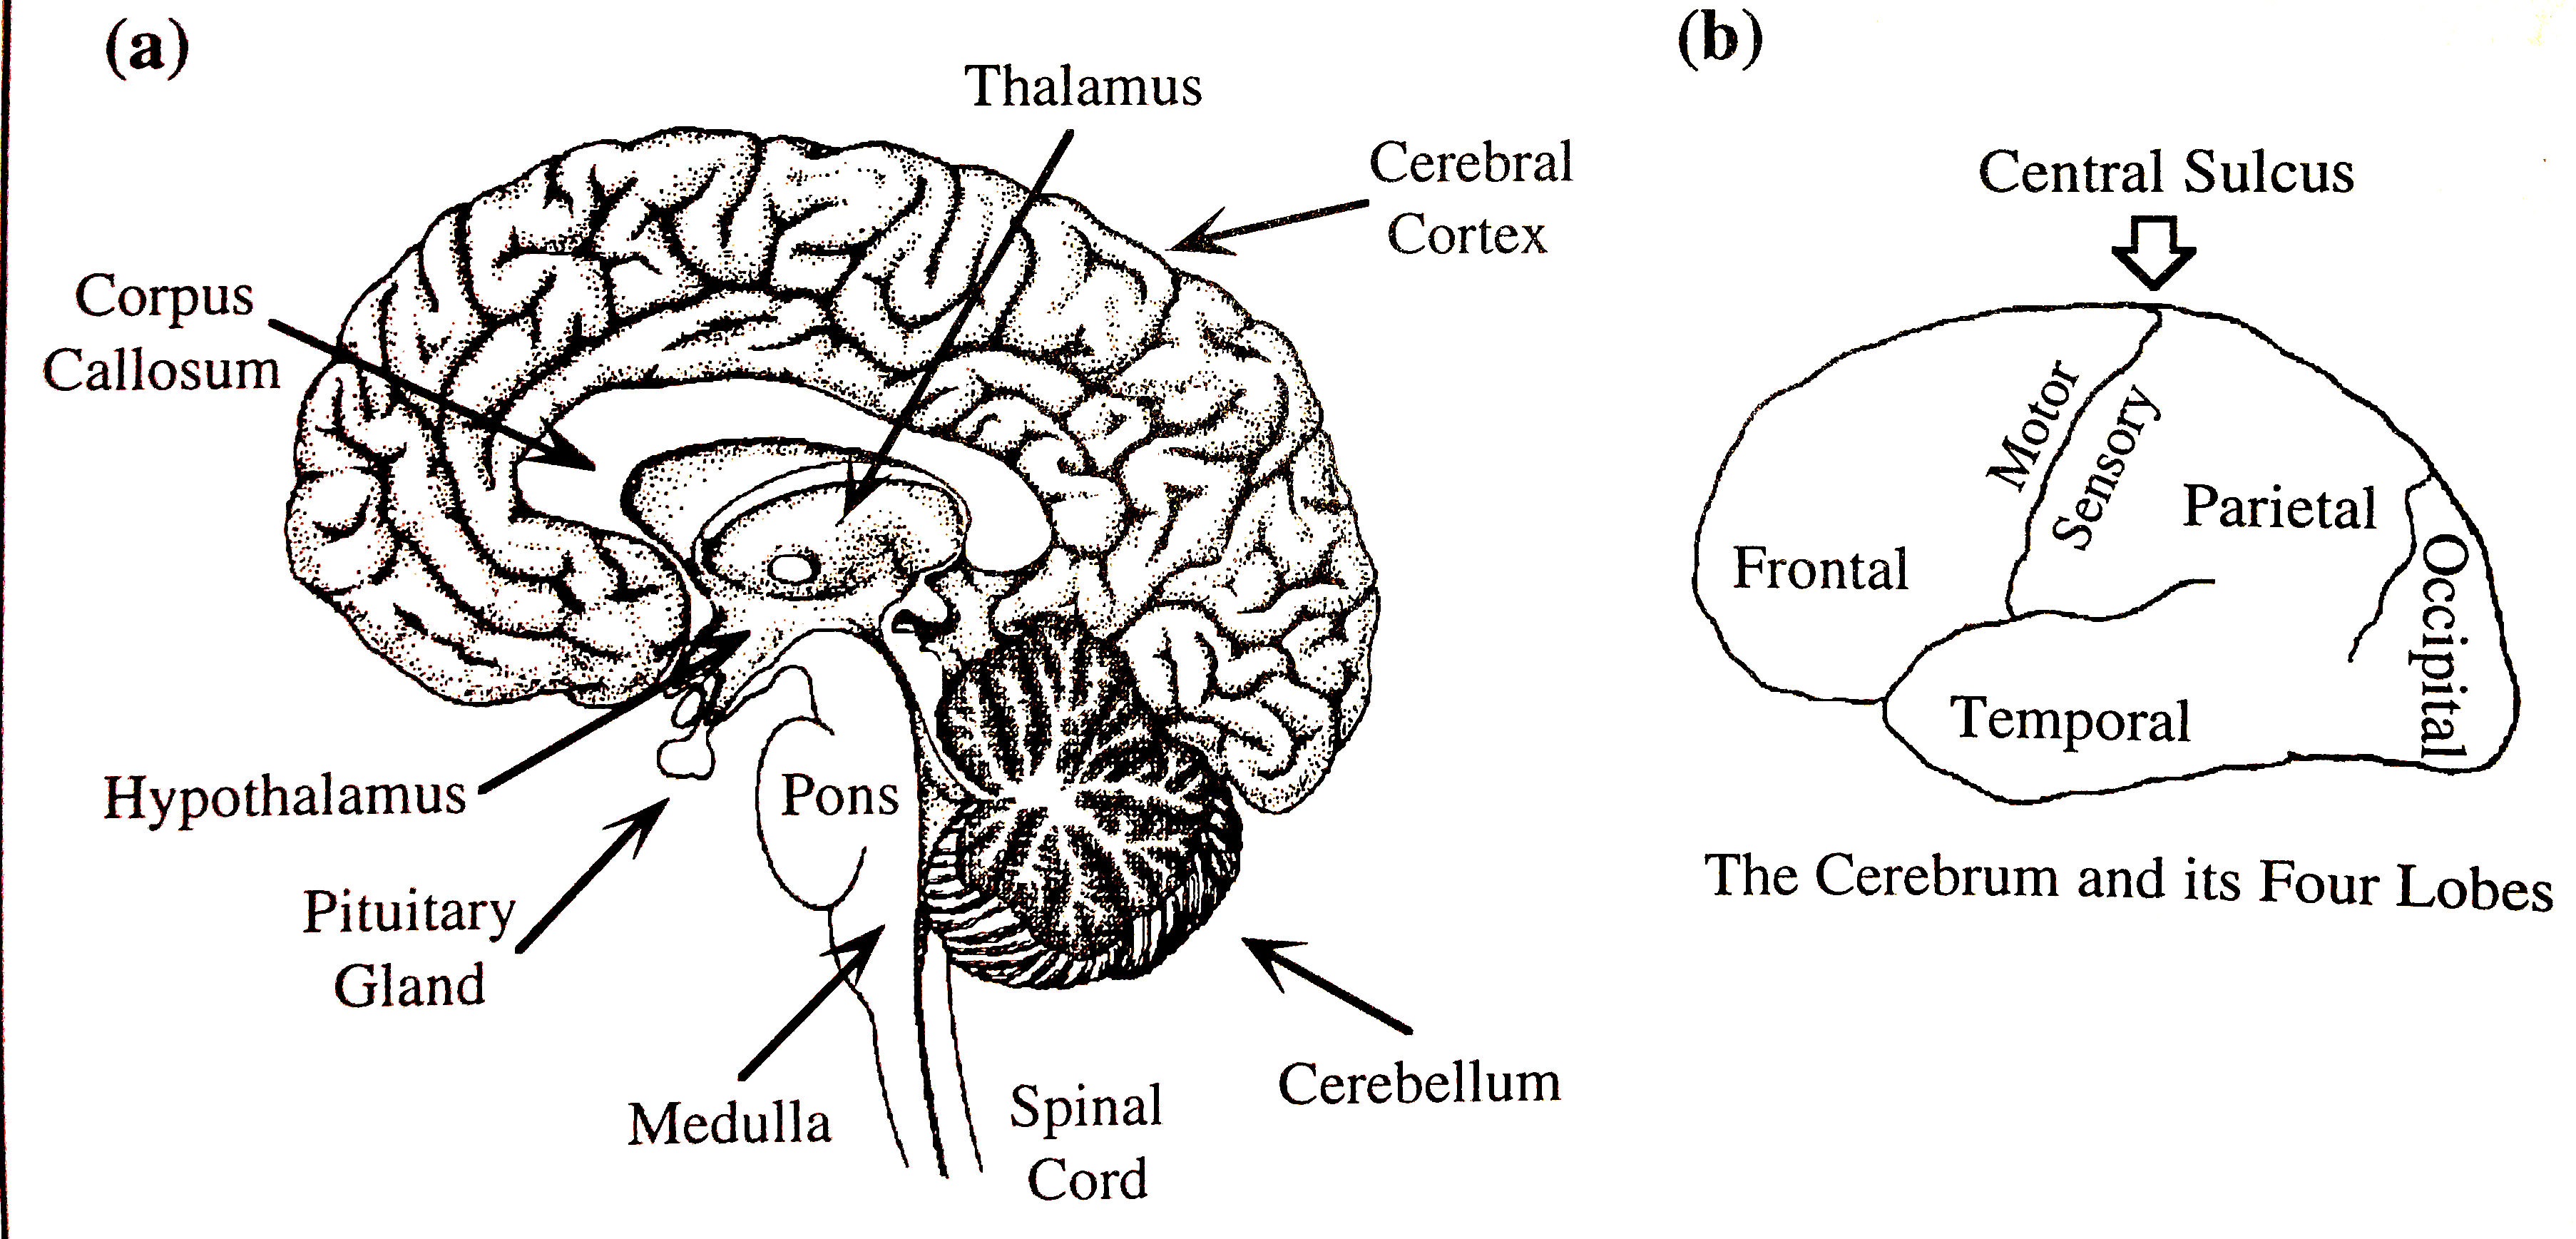
\includegraphics[width=0.7\textwidth]{brain.png} \label{brain}
\caption{Anatomical divisions of the vertebrate brain.}
\end{figure}
\indent The \textbf{central sulcus} is a prominent groove that separates the frontal lobes and parietal lobes. Anterior to the sulcus is the \textbf{motor cortex}, which controls the movement of individual muscles. Posterior to this sulcus is the \textbf{sensory cortex}, which detects sensations in various parts of the body. \\
\indent The \textbf{thalamus} is a relay station for much of the visual and auditory information from the environment. The \textbf{hypothalamus} is concerned with the visceral (subconscious) activities of the body. The \textbf{pituitary gland} is the master endocrine gland of the body\textemdash it receives information from the hypothalamus and sends out information to regulate different parts of the body. \\
\indent The \textbf{brainstem} contains the \textbf{midbrain}, \textbf{cerebellum}, \textbf{pons}, \textbf{medulla}, and the \textbf{reticular formation}, which in general coordinate motor and visceral activities. The midbrain detects movement and can direct the head and eyes towards that movement. It can also sense pleasure and pain. The cerebellum is responsible for the bulk of regulation and coordination of muscular activity. The pons and medulla coordinate visceral activities. The reticular formation, which is the core of the brainstem, is essentially an activating system designed to alert the brain. It also inhibits motor and sensory impulses and can induce sleep. Below the medulla is the spinal cord. 

\subsection{Control of Body Activity and the Neurovisceral Control}
A response that makes just one synaptic connection is referred to as a \textbf{monosynaptic reflex arc}, while a response that makes at least two synaptic connections is referred to as a \textbf{polysynaptic reflex arc}. \\
\indent The \textbf{autonomic} nervous system is part of the \textbf{efferent} division of the PNS, which can be further subdivided into the \textbf{sympathetic} and the \textbf{parasympathetic} systems. The \textbf{parasympathetic division} of the autonomic nervous system has nerve fibers which leave from the \textbf{sacral} portion of the spinal cord and from the midbrain (mesencephalon) and medulla (part of the rhombencephalon). Parasympathetic nerve impulses tend to increase the rate of digestion and lower the heart rate. The blood pressure is also lowered, and the pupils constrict. In general, the parasympathetic division conserves energy and helps in the restoration of various bodily functions. The parasympathetic division has both \textbf{preganglionic} and \textbf{postganglionic} nerve fibers. The cell bodies of the preganglionic neurons are found in the sacral region of the spinal cord and in the brainstem. The preganglionic nerve fibers are rather long, while the postganglionic nerve fibers are rather short. Both the preganglionic and the postganglionic nerve fibers in the parasympathetic division release ACh as the neurotransmitter. (Nerve fibers that release ACh as their neurotransmitter are called \textbf{cholinergic} nerve fibers. \\
\indent The most prominent nerve in the parasympathetic division is the \textbf{vagus nerve}, which innervates the heart, lungs, stomach, liver, small intestine, large intestine, and kidneys, among other organs. An overview of the parasympathetic nervous system is shown in \textbf{Fig. \ref{parasympathetic}}.\\
\begin{figure}[!ht]
\centering
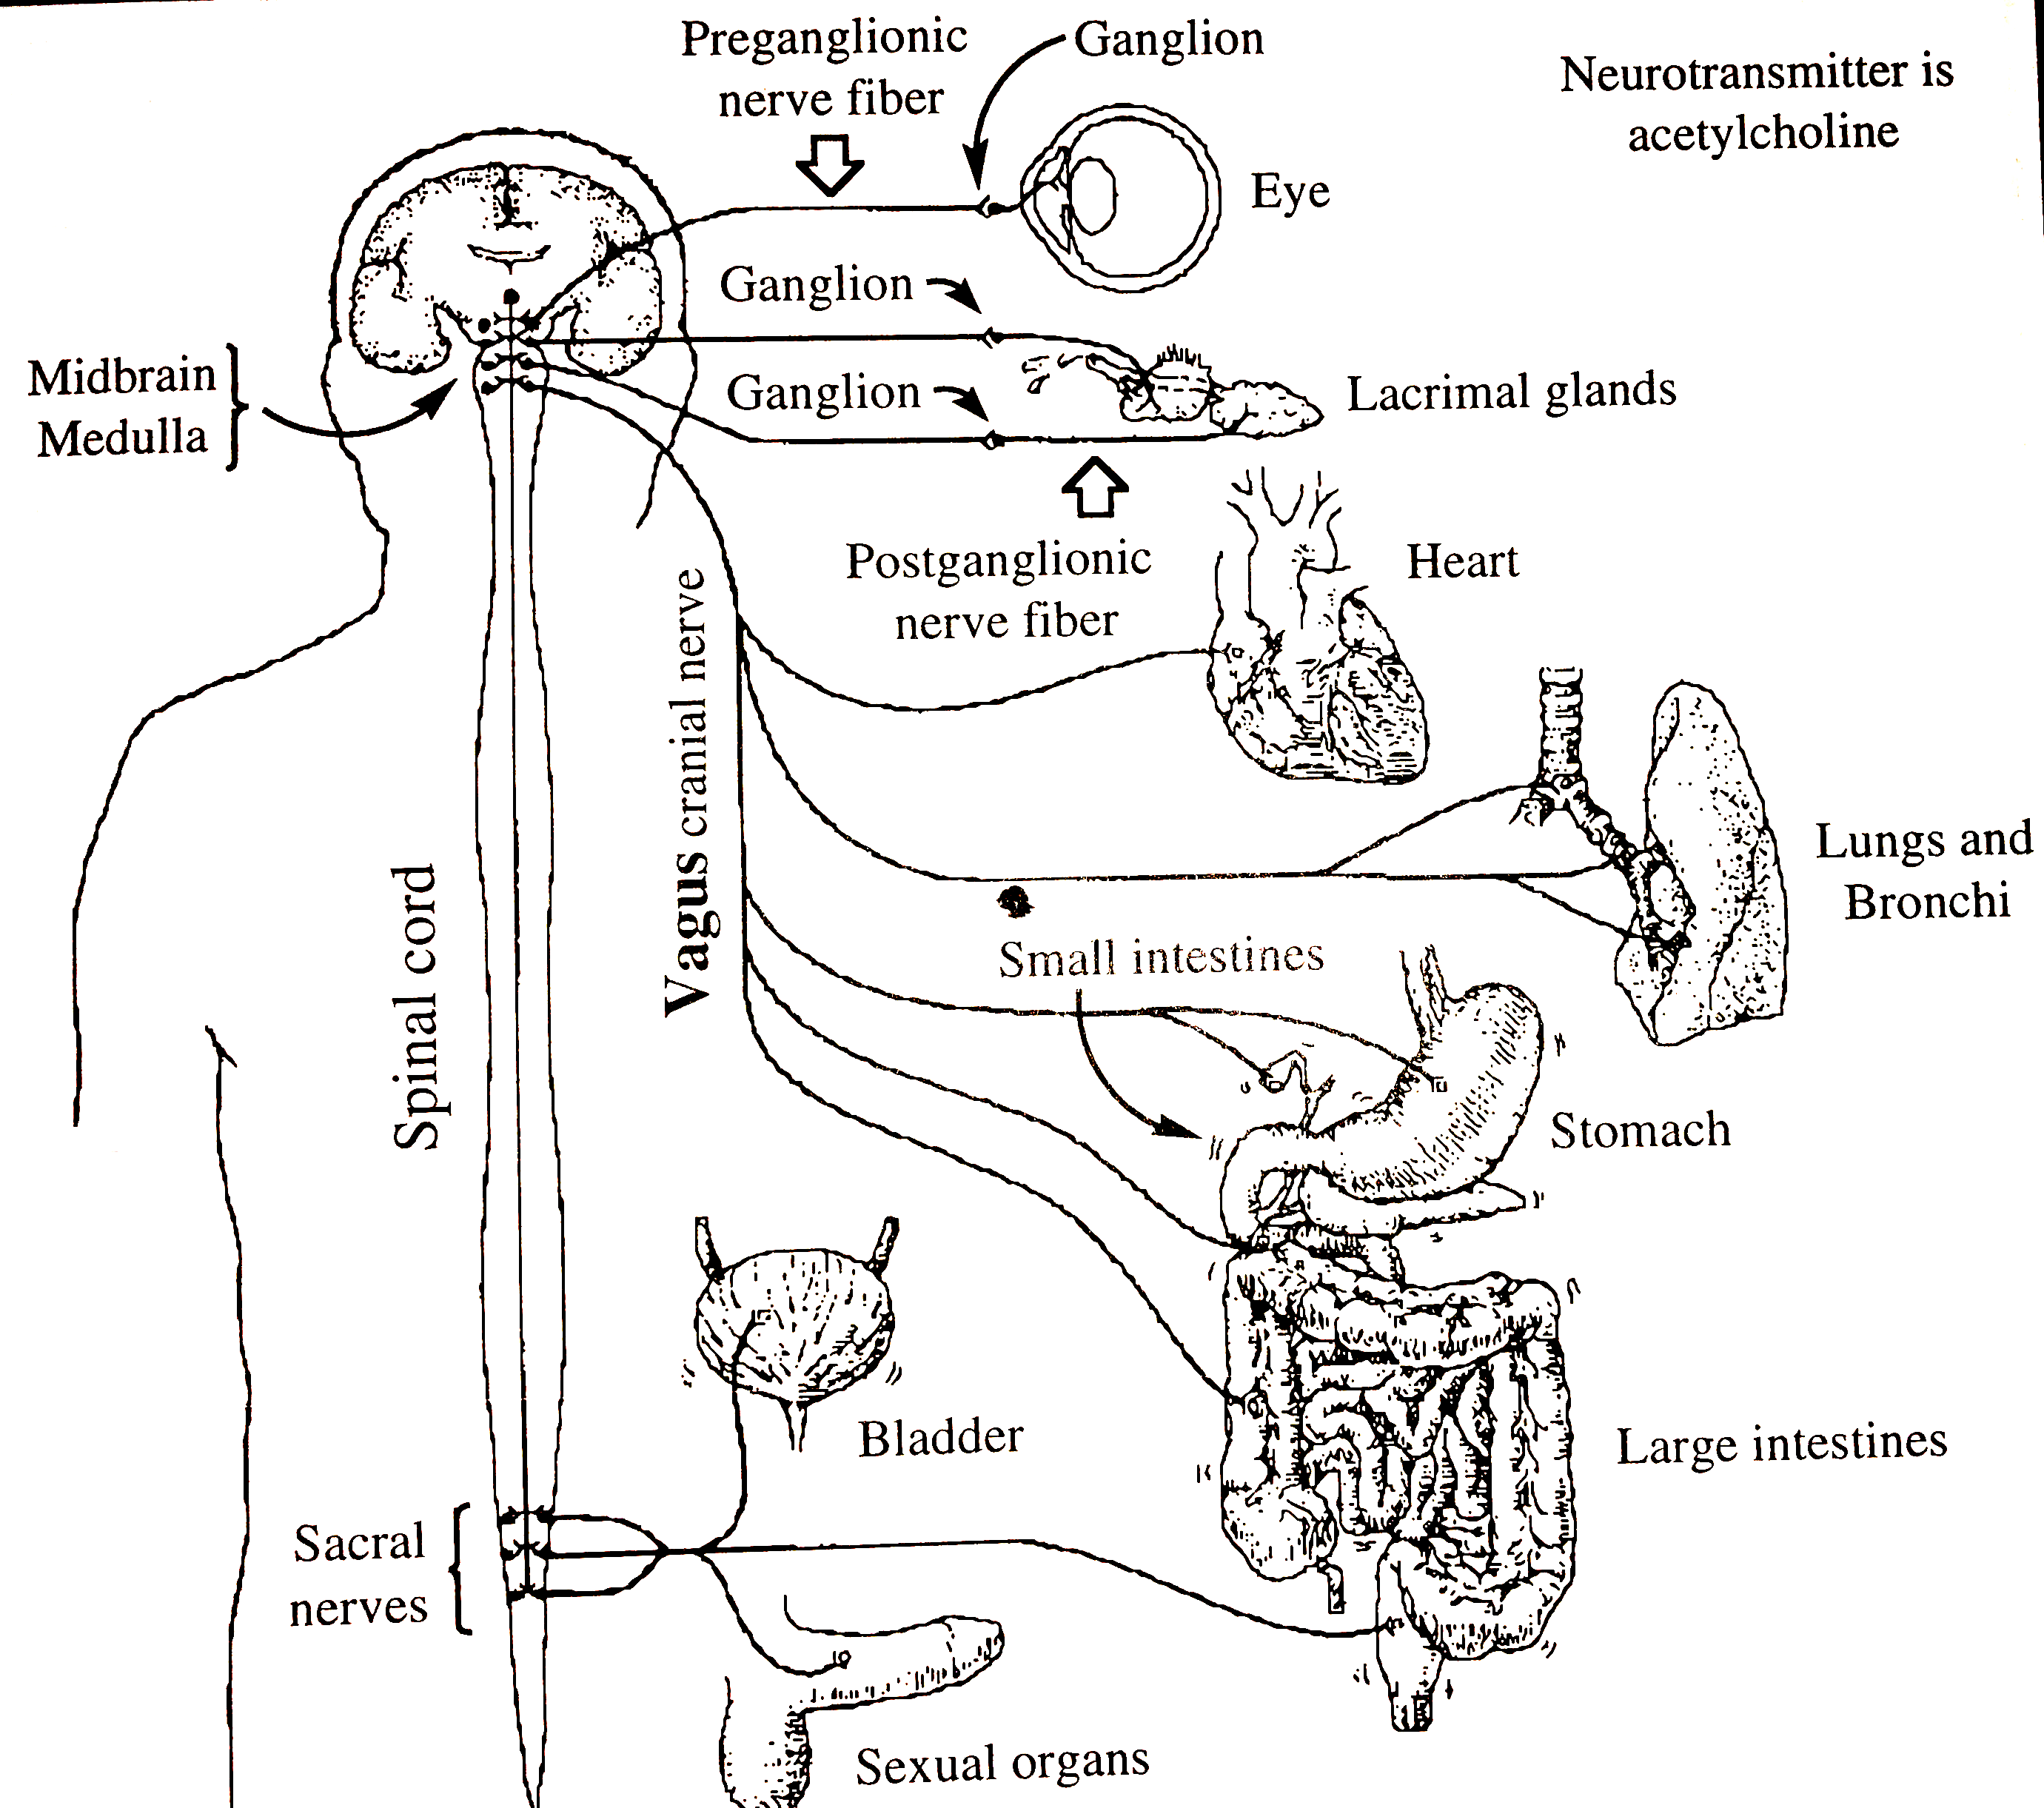
\includegraphics[width=0.7\textwidth]{parasympathetic.png} \label{parasympathetic}
\caption{Parasympathetic nerves and the parasympathetic division of the automatic nervous system.}
\end{figure}
\indent The sympathetic division of the autonomic nervous system has nerve fibers branching off from the \textbf{thoracic} and \textbf{lumbar} regions of the spinal cord. Sympathetic nerve fibers tend to condition the body for a `fight-or-flight' response. The heart rate increases, blood pressure elevates, pupils dilate, and the digestive functions decrease, all as a result of sympathetic nervous innervation. The nerve fibers leaving a synapse in a given ganglion are referred to as \textbf{postganglionic} nerve fibers. In the case of the sympathetic division the preganglionic nerve fibers tend to be short, while the postganglionic nerve fibers tend to be longer. The preganglionic fibers release ACh, while the postganglionic fibers release norepinephrine as their neurotransmitters.\\
\indent An important set of spinal nerves in the sympathetic division are the long preganglionic nerve fibers to the \textbf{adrenal medulla}. There are no postganglionic nerve fibers here\textemdash when the adrenal medulla is stimulated, both \textbf{norepinephrine} and \textbf{epinephrine} are released directly into the bloodstream. \\
\indent The \textbf{somatic} nervous system has some notable characteristics:
\begin{enumerate}
	\item Once the nerve fibers leave the CNS, they do not make a synapse until they have reached their effector organ.
	\item When the synapse is made at the effector organ, the neurotransmitter that is released is \textbf{acetylcholine}.
	\item The somatic nervous system innervates skeletal muscle. 
	\item Innervation of that skeletal muscle leads to excitation of the muscle itself. 
\end{enumerate}
\indent In contrast, the \textbf{autonomic} nervous system has some notable characteristics:
\begin{enumerate}
	\item Once the nerve fibers leave the CNS, they synapse with a ganglion before they make the final synapse with their effector organ.
	\item The preganglionic fibers in both the parasympathetic and sympathetic divisions released acetylcholine as the neurotransmitter. The postganglionic fibers in the parasympathetic division release acetylcholine; in the sympathetic division, norepinephrine is released.
	\item The autonomic nervous system innervates glands, and smooth and cardiac muscle. 
	\item The cells innervated by the autonomic nervous system can be either excitatory or inhibitory. 
\end{enumerate}
\indent The \textbf{adrenal medulla}, a specialized ganglion in the sympathetic division of the autonomic nervous system, is directly stimulated by a preganglionic fiber. This nerve fiber releases ACh, which causes the cells of the adrenal medulla to release epinephrine primarily and also norepinephrine. A review of the CNS and PNS is shown in \textbf{Fig. \ref{CNSPNS}}.
\begin{figure}[!ht]
\centering
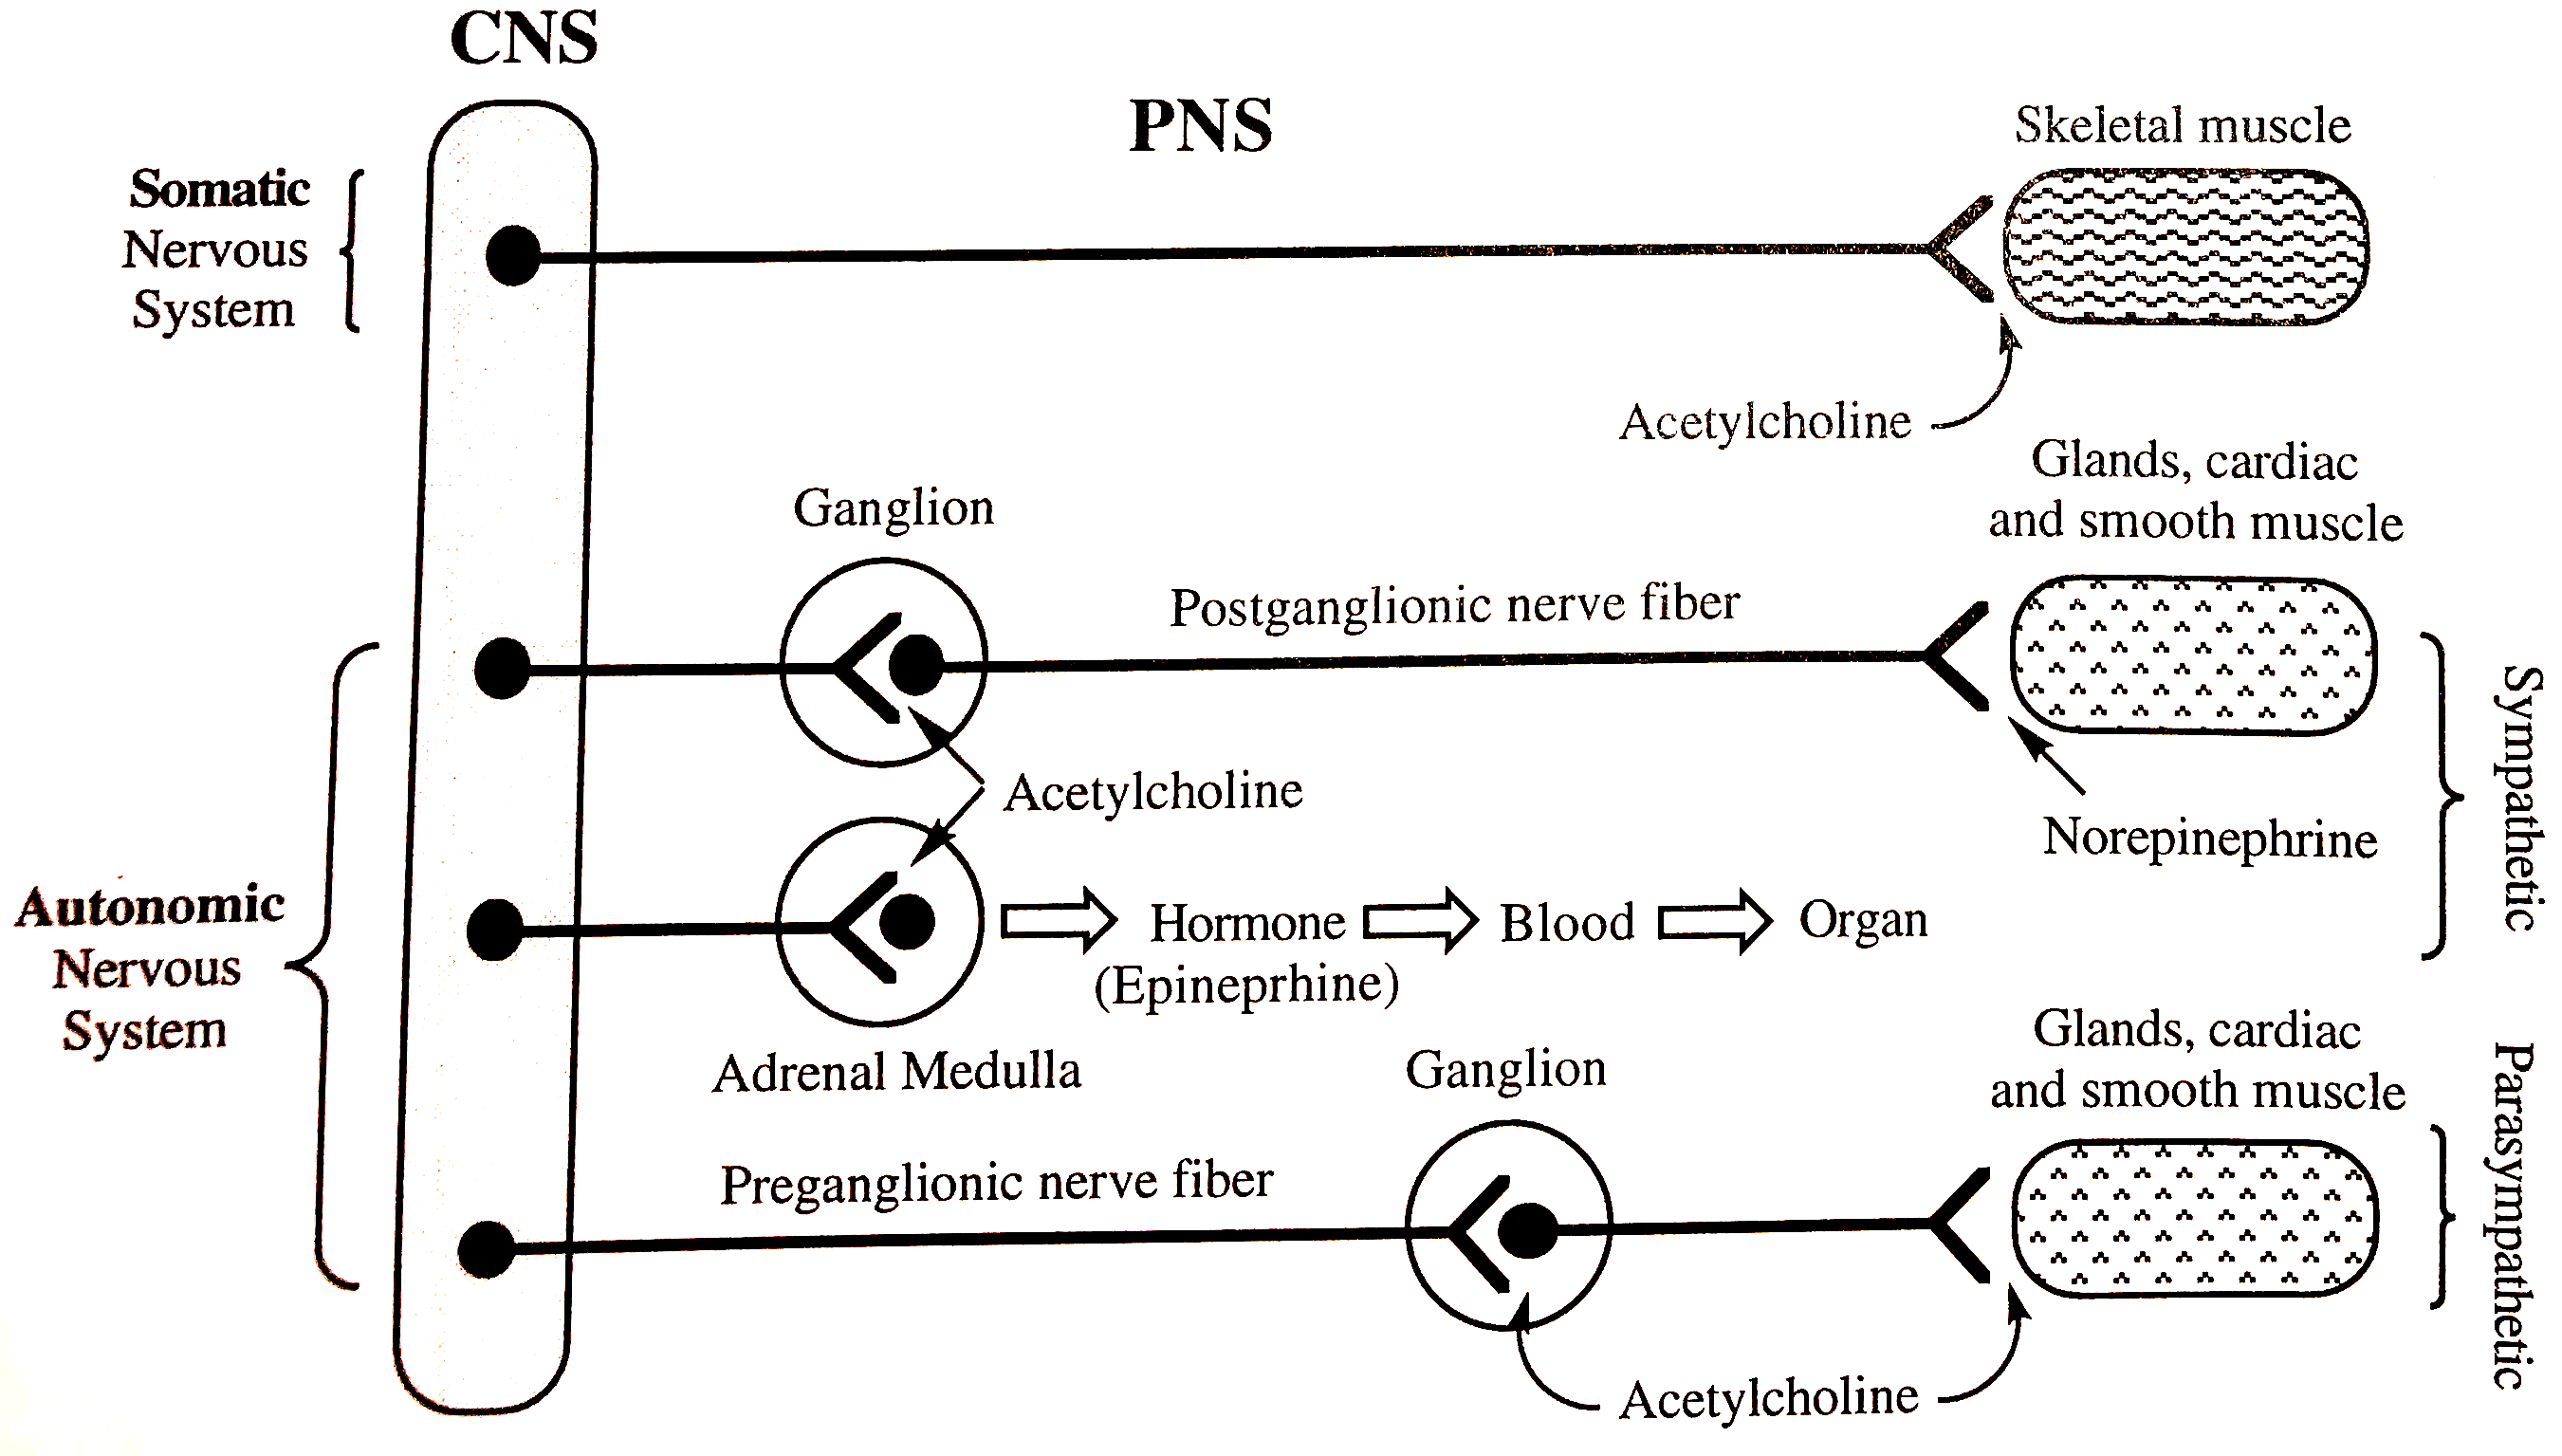
\includegraphics[width=0.7\textwidth]{CNSPNS.png} \label{CNSPNS}
\caption{CNS and PNS review.}
\end{figure}

\subsection{Receptors and Sensory Input}
\textbf{Nocirceptors} sense pain. In general, the things that are important in propagating signals in the nervous system are the frequency of action potentials, not the magnitude, as the magnitude of action potentials is always basically the same. All receptors essentially function on this basic principle. \textbf{Sensory adaptation} is the phenomenon where the body doesn't keep responding to repeated stimuli. 

\subsection{Cardiovascular Anatomy}
The function of the \textbf{circulatory system} is to bring nutrients and oxygen to the tissues of the body while simultaneously removing waste products from those same tissues. Because the circulatory system is continually flowing, it also helps to maintain body temperature. Also, the circulatory system can act as a means to transport hormones to various locations within the body. The blood that is pumped from the right heart to the lungs and back to the left heart is called the \textbf{pulmonary circulation} while the blood that is pumped from the left heart to the rest of the tissues and back to the right heart is called the \textbf{systemic circulation}. Both these circulations lie in series with right another.\\
\indent Deoxygenated blood passes from the right atrium into the right ventricle, and then is pumped to the \textbf{pulmonary artery} and to the lungs where it is oxygenated. The oxygenated blood then returns to the left heart by the \textbf{pulmonary veins}. The blood enters the left atrium and passes into the left ventricle where it is pumped out the \textbf{aorta} and to the branching arteries, arterioles, and capillaries. It is at the level of the capillaries that the blood exchanges nutrients and oxygen for waste products created by metabolism. Deoxygenated blood passes from the capillaries to \textbf{venules} and then to larger veins, and eventually to the \textbf{superior} and \textbf{inferior vena cava}, which enter the right atrium. The general anatomy of the hear is shown in \textbf{Fig. \ref{heart}}.\\
\begin{figure}[!ht]
\centering
\includegraphics[width=0.7\textwidth]{heart.png} \label{heart}
\caption{Anatomical landmarks of the heart.}
\end{figure}
\indent As the left ventricle contracts (\textbf{systole}), it propels blood out the aorta and into the arteries with a pressure of about 120 mmHg. After contraction takes place and ventricles begin to relax (\textbf{diastole}) and fill with blood, the pressure in the arteries is about 80 mmHg. Since blood is under a lot of pressure, the arteries have to be durable. They have thick walls composed of \textbf{smooth muscle} and \textbf{connective tissue} that contain both \textbf{collagenous} and \textbf{elastic} fibers.\\
\indent The lumen of blood vessels are lined with epithelial cells called \textbf{endothelial cells}. Damage to these cells by the pulsating arterial pressure or even by abrasive substances in the blood can lead to \textbf{atherosclerosis}. Once these cells are damaged, cholesterol can build up at the site of the lesion and a plaque will form. During the later stages, the arteries become `hardened' from the layers of deposition, and this is referred to as \textbf{arteriosclerosis}. \\
\indent Regulation of the circulatory system is controlled by the sympathetic and parasympathetic divisions of the autonomic nervous system. The sympathetic division is the more important of the two. Besides nervous control of blood flow, there is also humoral control from the action of ions or hormones and local control at the level of the individual tissues from various metabolites.\\
\indent The wall of capillaries are composed of a unicellular layer of endothelial cells. Surrounding these cells is a basement membrane. However, there is no connective tissue or smooth muscle. The capillary itself is just large enough for a RBC to squeeze through. At the entrance to the capillary bed is a \textbf{precapillary sphincter} composed of smooth muscle which helps to regulate the flow of blood to the area.\\
\indent Valves are very important in maintaining the directionality of blood flow. There are atrioventricular valves between the atria and the ventricles, which close as the ventricles are contracting, and also the pulmonary valve and aortic valves that close when blood flows out of the pulmonary artery and the aorta, respectively. The atrioventricular valves do not invert because of tendinous cords called \textbf{chordae tendineae} that hold them in place. \\
\indent Located near the junction of the superior vena cava and the right atrium is the \textbf{sinoatrial node} (SA node), which is the pacemaker of the heart. The SA node is the point of origin for the electrical impulse that propagates through the rest of the heart. Located in the lower portion of the right atrium and near the right ventricle is the \textbf{atrioventricular node} (AV node). Impulses from the SA node also spread to the AV node and then from the AV node through a collection of fibers called the \textbf{bundle of His}. Branches of the bundle of His surround the ventricles, and when this bundle receives an impulse, it causes the ventricles to contract and eject blood to the pulmonary and systemic systems. \\
\indent Sympathetic nerves and norepinephrine can be released at the SA node to increase the rate of the heart. \textbf{Cardiac output} is the amount of blood that is pumped per minute by each of the two individual ventricles of the heart:
\begin{equation}
\begin{split}
\text{Cardiac Output}=\left(\text{Stroke Volume}\right)\left(\text{Heart Rate}\right)
\end{split}
\end{equation}
\noindent where stroke volume is measured in liters per beat and heart rate is measured in beats per minute. \textbf{Poiseuille's Law} describes the flow rate of a fluid in blood vessels:
\begin{equation}
\begin{split}
\text{Flow Rate}=\Delta P \frac{\pi R^4}{8\eta L}=\left(P_1-P_2\right) \frac{\pi R^4}{8\eta L}
\end{split}
\end{equation}
\noindent where $\Delta P$ is the pressure drop, $R$ is the radius of the blood vessel, $\eta$ is the coefficient of viscosity, and $L$ is the length of the tube. The actual formula for Poiseuille's Law is not so important\textemdash rather, understanding how flow rate changes with each of these physical variables is much more important. Meanwhile, \textbf{Fick's Law} describes the net flux/net rate of diffusion $J$ in mol/sec:
\begin{equation}
\begin{split}
J=-DA\frac{\Delta C}{\Delta x}
\end{split}
\end{equation}
\noindent $D$ is the diffusion coefficient (a proportionality constant), $A$ is the area of the plane of interest, and $\Delta C/\Delta x$ is the concentration gradient across that plane. The minus sign indicates the direction of the flux or diffusion. \\
\indent \textbf{Osmolarity} is basically normality. For example, if we had a 1M solution of glucose, it would have a concentration of 1 osmol per liter. If we have a 1M solution of sodium chloride, this has a concentration of 2 osmols per liter (one from the \ce{Na+} ion and one from the \ce{Cl-} ion). 

\subsection{Lymphatic System}
The \textbf{lymphatic system} lies parallel to the systemic and pulmonary circulations. It collects the excess fluid that leaks into the interstitial space from the capillaries and returns it by way of the vena cava back to the circulatory system. Lymph nodes located along the lymphatic system help to filter out foreign particles that could potentially lead to disease. If the lymph flow through the lymphatic system were blocked, \textbf{edema} would result. This is simply an increase in the interstitial fluid.

\subsection{Blood Clotting}
Blood clotting occurs via a \textit{cascade process}. As a general overview, \textbf{thrombin} is a serine protease involved in blood clotting. There are two pathways in blood clotting\textemdash the \textbf{intrinsic route} (due to contact with some abnormal surface) and the \textbf{extrinsic route} (due to trauma to the tissue). In blood clotting there are more than 15 different factors involved, and about 8 or so of them are serine proteases. \\
\indent In \textbf{Fig. \ref{blood_clotting}}, we show the intrinsic and extrinsic pathways. The subscript `a' means that we are dealing with the \textit{active} form of the molecule. Factor IX will be converted to Factor IX\textsubscript{a} by some \textbf{intrinsic factor}. Factor IX\textsubscript{a} will be the trigger which will convert Factor X to Factor X\textsubscript{a}. From the \textbf{extrinsic} portion of this scheme, we start with some tissue factor which converts Factor VII to Factor VII\textsubscript{a}. Factor VII\textsubscript{a} can also bring about the conversion of Factor X to Factor X\textsubscript{a}. It is then Factor X\textsubscript{a} (and also an additional factor, Factor V\textsubscript{a}) that is involved in the conversion of \textbf{prothrombin} (Factor II) to \textbf{thrombin} (Factor II\textsubscript{a}). Thrombin converts \textbf{fibrinogen} (Factor I) to \textbf{fibrin} (Factor I\textsubscript{a}). These fibrin fibers are then cross-linked by Factor XIII\textsubscript{a}, which is an enzyme called \textbf{transglutaminase} to form the mature cross-linked fibrin clot. 
\begin{figure}[!ht]
\centering
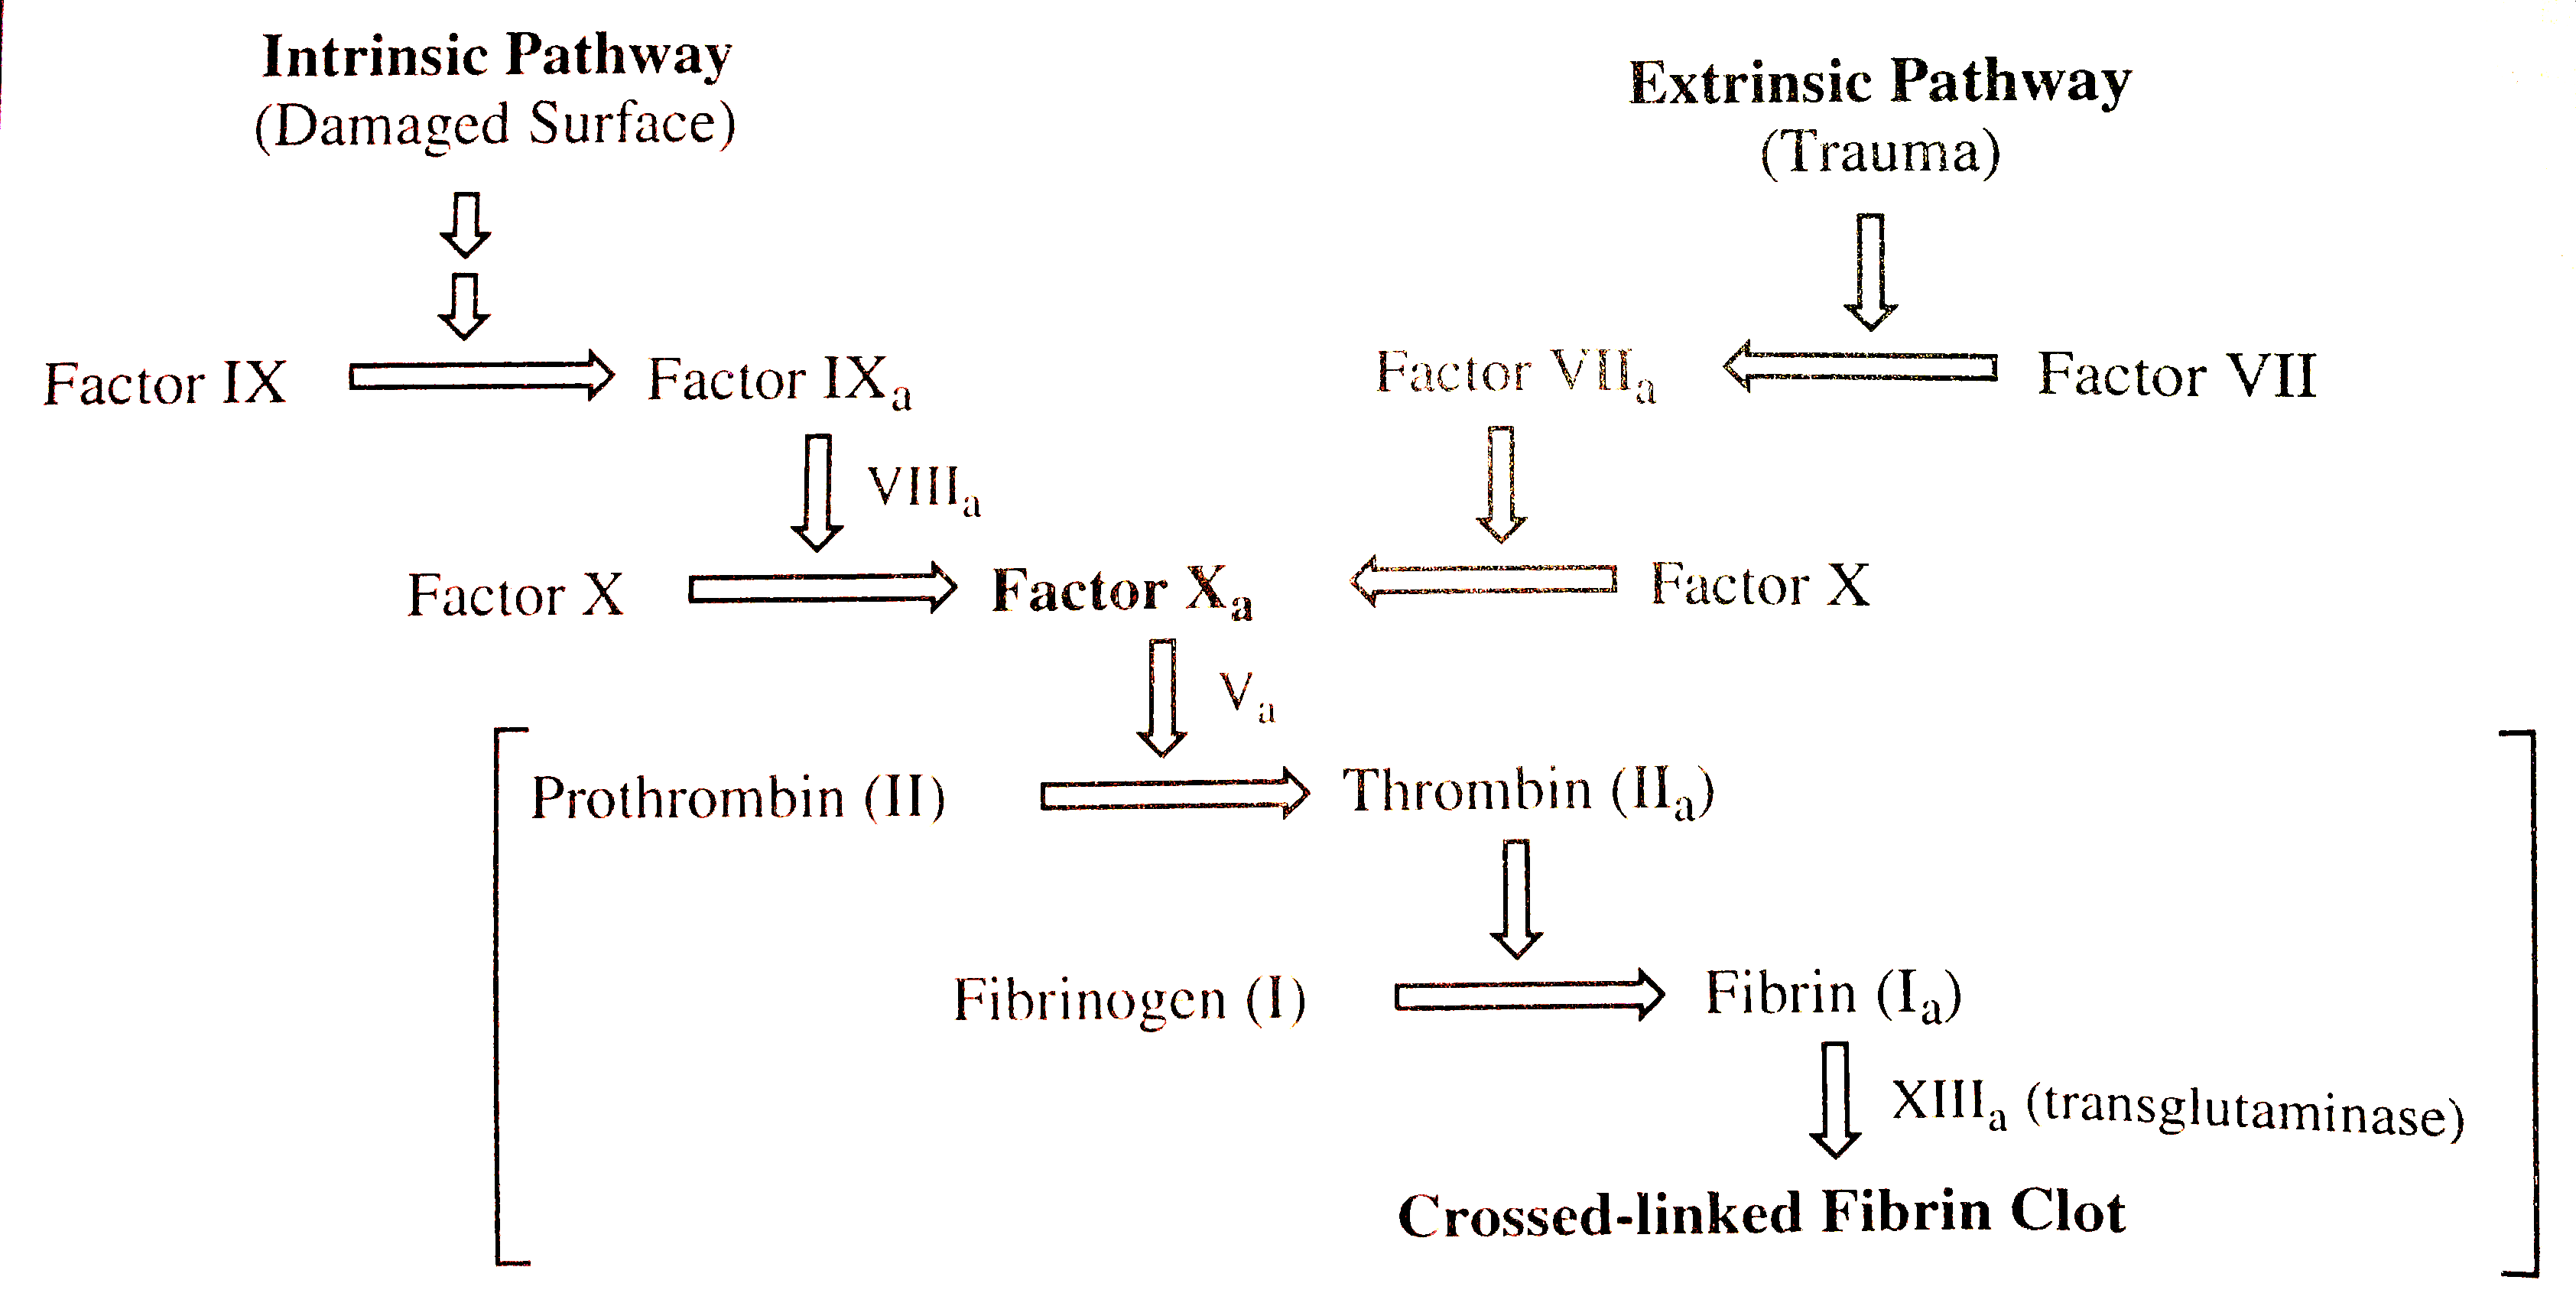
\includegraphics[width=0.7\textwidth]{blood_clotting.png} \label{blood_clotting}
\caption{The intrinsic and extrinsic pathways of blood clotting.}
\end{figure}
\noindent \textbf{Vitamin K} is a fat-soluble vitamin, and it is important for blood clotting. This is because prothrombin exists in an even earlier form called \textit{preprothrombin}, which has certain Glu residues that are carboxylated by a carboxylase enzyme. This carboxylase enzyme has an absolute requirement for Vitamin K. Therefore, in the presence of Vitamin K, \ce{HCO_{3}-}, and the carboxylase enzyme, we can convert preprothrombin to prothrombin. This structure now has great affinity for divalent ions such as \ce{Ca^2+}, and is therefore a good chelating agent. Therefore, the essentials for the clotting process to take place is the (a) platelet membrane, (b) enzymes, (c) \ce{Ca^2+}, (d) an auxiliary factor, Factor V\textsubscript{a}, and (e) the substrate prothrombin. \\
\indent Thrombin can now act as a proteolytic enzyme that converts \textit{fibrinogen} to \textit{fibrin}. Fibrinogen is a large soluble protein. Its solubility is due to an excess of negatively charged amino acids (i.e. Glu, Asp, Tyr-\ce{SO_4}), particularly in the central domain of the molecule. The net charge in the central domain of the fibrinogen is -8, while the net charge at the terminal ends is -4. In general, if very large molecules have a net charge of zero, they will tend to come together. However, if we have an excess of charge (as is the case with fibrinogen), the molecules will repel one another. Thus, in order to convert the soluble fibrinogen to the insoluble fibrin, we can remove the portion of the molecule contributing all the negative charge. Indeed, when fibrinogen is converted to fibrin, we find that 4 Arg-Gly bonds are broken in the central domain, releasing four peptides containing an excess of negative charge. Once these `fibrinopeptides' are released, the overall net charge in the central domain now becomes +5 (originally -8 in fibrinogen). The fibrin monomer that is now formed has the ability to interact with other fibrin monomers through electrostatic interactions between the terminal (negatively charged) and central (positively charged) regions of the polypeptide\textemdash the resulting aggregation is called a \textbf{fibrin (soft) clot}. \\
\indent To make the soft clot into a hard clot, the enzyme transglutaminase (Factor XIII\textsubscript{a}) cross-links the monomers. Once the damaged area has been repaired, a serine protease called \textbf{plasmin} hydrolyzes specific regions in the fibrin clot in order to dissolve it into smaller peptide fragments (to remove the clot). \textbf{Tissue plasminogen activator (TPA)} converts \textbf{plasminogen} into this active protease. 

\subsection{The Lungs}
When we breathe air, it first enters through the nose/mouth, passes from the oral cavity to the \textbf{pharynx}, into the \textbf{larynx}, and then down the \textbf{trachea}. At the end of the trachea, the air passes into two tubular passageways called \textbf{bronchi}. One bronchi enters into each lung and continues to divide into smaller passageways called \textbf{bronchioles}, eventually ending in the functional units of the lungs called the \textbf{alveoli}. Each alveolus consists of a single layer of epithelial cells juxtaposed to a very thin basement membrane. Surrounding each single alveolus is a capillary network.\\
\indent At equilibrium, the number the \ce{O2} molecules dissolving in water will equal the number of \ce{O2} molecules leaving the water. This means the partial pressure of oxygen in the gas phase (air) is equal to the partial pressure of oxygen in the liquid phase (water):
\begin{equation}
\begin{split}
\boxed{\left(P_{\text{O\textsubscript{2}}}\right)_{\text{gas}}=\left(P_{\text{O\textsubscript{2}}}\right)_{\text{liquid}}}
\end{split}
\end{equation}
\noindent The \textbf{epithelial cells} that line the lumen of the passageways to the end of the bronchioles have \textbf{cilia} which are continually beating towards the pharynx. Scattered among these epithelial cells are glands that secrete \textbf{mucus}, which is important to trap and foreign matter and get rid of it as the mucus is moved upward towards the oral cavity. The upper passageways of the respiratory tract maintain their opening by means of \textbf{cartilage rings}. Smooth muscle is found in almost all areas of the respiratory tract where there's no cartilage. \textbf{Asthma} is caused by allergic hypersensitivity to airborne antigens that have entered the respiratory tract. The direct result is to cause the mast cells within the bronchioles to release a number of different substances that cause the smooth muscle surrounding bronchioles to spasm and constrict. \\
\indent The lungs are encased in the pleural membrane. The \textbf{visceral pleura} covers the lungs, while the \textbf{parietal pleura} adheres to the diaphragm and chest wall. Between the visceral pleural and parietal pleura is the \textbf{intrapleural space} which contains a watery fluid. During inspiration, the muscles of the diaphragm contract and pull the diaphragm down, enlarging the thoracic cage and expanding the lungs. This creates a subatmospheric pressure in the alveoli, which causes air to rush down its pressure gradient from the atmosphere into the lungs. During expiration, the thoracic cage and lungs return to normal, and air in the alveoli is compressed and forced out through the passageways of the respiratory tract. If the lungs were to become separated from the visceral pleura, they would collapse, causing \textbf{pneumothorax}. This is because they have no anatomical structures to maintain rigidity. \\
\indent As deoxygenated blood comes back from the tissues, it enters the right atrium via the superior and inferior vena cava and passes into the right ventricle, where it is pumped to the lungs via the pulmonary artery. In the alveoli, both \ce{O_2} and \ce{CO_2} diffuse down their respective concentration gradients from the capillaries to the alveoli. This means that the oxygen enters the blood and carbon dioxide leaves the blood. The blood then becomes oxygenated, comes back to the heart via the pulmonary vein, and passes from the left atrium to the left ventricle and then pumped to the tissues via the aorta. Oxygen can travel/dissolve in the blood itself, but it's pretty insoluble in water/blood. Rather, most oxygen is transported by being bound to a transport protein in erythrocytes called \textbf{hemoglobin (Hb)}. Hb has four polypeptide units, each of which has a \textbf{heme} prosthetic group with an iron atom in the center in the ferrous \ce{Fe^2+} state. Thus, each hemoglobin molecule can take up to four \ce{O_2} molecules. \\
\indent Hb is dependent on pH and temperature\textemdash if we were to decrease the pH of the blood or increase the temperature, then less hemoglobin will be saturated with oxygen. This is what happens when you exercise. Similarly, this shift in the oxygen saturation curve happens when a byproduct of glycolysis, \textbf{2,3-bisphosphoglycerate (2,3-BPG)}, binds go hemoglobin.\\
\indent \ce{CO_2} can be carried in the blood by either (1) dissolving in the plasma and RBCs, (2) binding to a specific site on the hemoglobin molecule, or (3) in the form of bicarbonate ions (\ce{HCO_{3}-}). Most of the \ce{CO_2} is carried in the blood in the form of bicarbonate ions. 

\subsection{The Gastrointestinal Tract}
The gastrointestinal (GI) system includes the mouth and associated salivary glands, esophagus, stomach, small intestine, large intestine, and certain aspects of the liver and pancreas. Starch, characteristic of plant cells, and glycogen, characteristic of animal cells, are hydrolyzed within the digestive trace by \textbf{amylases}. Upon hydrolysis, both polymers release glucose. \textbf{Cellulose} is found within the cell walls of plants; the enzyme \textbf{cellulase} can hydrolyze cellulose into its constituent glucose residues.
\begin{equation}
\begin{split}
\text{Starch}\xrightarrow[\textbf{Amylase}]{} \text{Glucose}, \quad \text{Cellulose}\xrightarrow[\textbf{Cellulase}]{\text{An example of bacterial symbiosis}} \text{Glucose}
\end{split}
\end{equation}
\noindent \textbf{Proteases} can hydrolyze proteins to their constituent amino acid residues. Of the 20 canonical amino acids, we need to obtain 9 of them in our diet, which are thus referred to as \textbf{essential amino acids}. The rest we can synthesize ourselves. Fat cellls (adipocytes) store triacylglycerols (i.e. fats) that are hydrolyzed into fatty acids and glycerol by the enzyme \textbf{lipase}.\\
\indent In the small intestine, the innermost layer is a convoluted layer of epithelial cells, with endocrine cells and ducts from external exocrine glands like the pancreas and liver scattered throughout that can release hormones into the blood and influence other cells in the GI tract. Both the parasympathetic and sympathetic nerves of the autonomic nervous system innervate the GI system; the more important nerves stem from the \textbf{parasympathetic} system. Recall that the parasympathetic nerves are more active during times of relaxation and digestion, while the sympathetic nerves are more active during times of `fight or flight.' \\
\indent As food is swallowed and passed into the pharynx, access to the nasal cavity is closed; a flap of tissue called the \textbf{epiglottis} covers the opening to the \textbf{larynx} and prevents food from entering into this passageway to protect the airway. The swallowing reflex is controlled by centers in the medulla. \\
\indent As food boluses pass through, the smooth muscles surrounding the epithelial cells contract in perstaltic waves, and this is referred to as \textbf{peristalsis}, controlled by the action of the parasympathetic division and by the action of hormones. \\
\indent Once the food reaches the stomach, a \textit{sphincter} (circular muscle) called the \textbf{gastroesophageal sphincter} contracts and prevents regurgitation of the food back into the esophagus. If this sphincter were not closed off, stomach acid would enter the esophagus and irritate the nerve endings in the smooth muscle, causing a burning sensation referred to as heartburn. In the stomach, there are four major types of secretion. \textbf{Mucus} is secreted by \textbf{surface cells} and acts to protect the lining of the stomach and lubricate the food. \textbf{Gastrin}, located in the endocrine cells in the lower portion of the stomach, is secreted in response to protein entering into the stomach. This hormone stimulates the secretion of \ce{HCl} and pepsinogen. \textbf{\ce{HCl}} at a pH of about 1 is secreted by \textbf{parietal cells}, while \textbf{pepsinogen} is secreted by the \textbf{chief cells}. Parietal cells and chief cells are located in the \textbf{gastric pits} that line the epithelium of the stomach. Pepsinogen is the inactive form of the peptidase enzyme \textbf{pepsin} that becomes activated by \ce{HCl} and also by a positive feedback loop and auto-activation once pepsinogen reaches the stomach. \\
\indent In addition to secreting \ce{HCl}, the parietal cells also secrete a glycoprotein called \textbf{intrinsic factor}. This glycoprotein is important because it complexes with vitamin B\textsubscript{12} and is then absorbed by the intestinal epithelial cells and transported by the bloodstream. Vitamin B\textsubscript{12} is important in erythrocyte formation. If too much acid is secreted into the stomach, \textbf{ulcers} can occur in the stomach and small intestine. Ulcers are erosions of the walls of these organs, and if they are extensive, they can cause bleeding. \textbf{Histamine} is a powerful stimulant that causes \ce{HCl} to be released into the lumen of the stomach, and so compounds like \textbf{cimetidine} inhibit the binding of histamine to its receptor on parietal cells. This effectively reduces the amount of \ce{HCl} secreted in the lumen of the stomach. \\
\indent Roughly $90\%$ of digestion and absorption that takes place in the GI tract occurs in the small intestine, which acts to neutralize the acid which has been secreted by the stomach and to further digest and absorb food particles. Distension of the small intestine also causes the hormone \textbf{cholecystokinin (CCK)} to be released from the intestinal mucosa. CCK diffuses through the bloodstream to the pancreas where it causes the pancreas to release digestive enzymes. The hormone \textbf{secretin} is released from the small intestine in response to the entering chyme from the stomach. Secretin is also absorbed by the blood and is transported to the pancreas where it causes the release of bicarbonate ion and other fluids.\\
\indent The \textbf{pancreas} not only has endocrine cells that secrete insulin and glucagon, but also contains secreting structures called \textbf{acini} that secrete a fluid into the small intestine which has a high \textbf{bicarbonate} conent that is rather alkaline, which reacts with the stomach acid to product carbonic acid, which then decomposes into carbon dioxide and water. \\
\indent The liver has many functions, one of which is to synthesize \textbf{bile} that is concentrated and stored in the \textbf{gallbladder}. Bile contains a major pigment called \textbf{bilirubin}, which is the breakdown product of hemoglobin. It also contains \textbf{bile salts} which are important in the digestion and absorption of fats. When bile is released from the gallbladder, it passes down a duct that joins with the pancreatic duct, through a constriction called the \textbf{sphincter of Oddi}, and empties into the small intestine. Bile acts to emulsify fats, which basically means just decreasing their surface tension in order to break them up into smaller sizes, making it easier to absorb. The presence of fats in the small intestine releases CCK which then acts on the gallbladder and causes contraction, and on the sphincter of Oddi and causes relaxation, so the bile can pass into the lumen of the small intestine. \\
\indent Remember that the \ce{Na+}-glucose symport is on the apical side of the epithelial cells in the small intestine (the side facing the lumen), while the \ce{Na+}-\ce{K+} antiport pump is on the basolateral side facing the blood. There's also a glucose passive transporter on the basolateral side to allow glucose to naturally enter the blood according to its concentration gradient. This is shown in \textbf{Fig. \ref{transport_systems}}.\\
\begin{figure}[!ht]
\centering
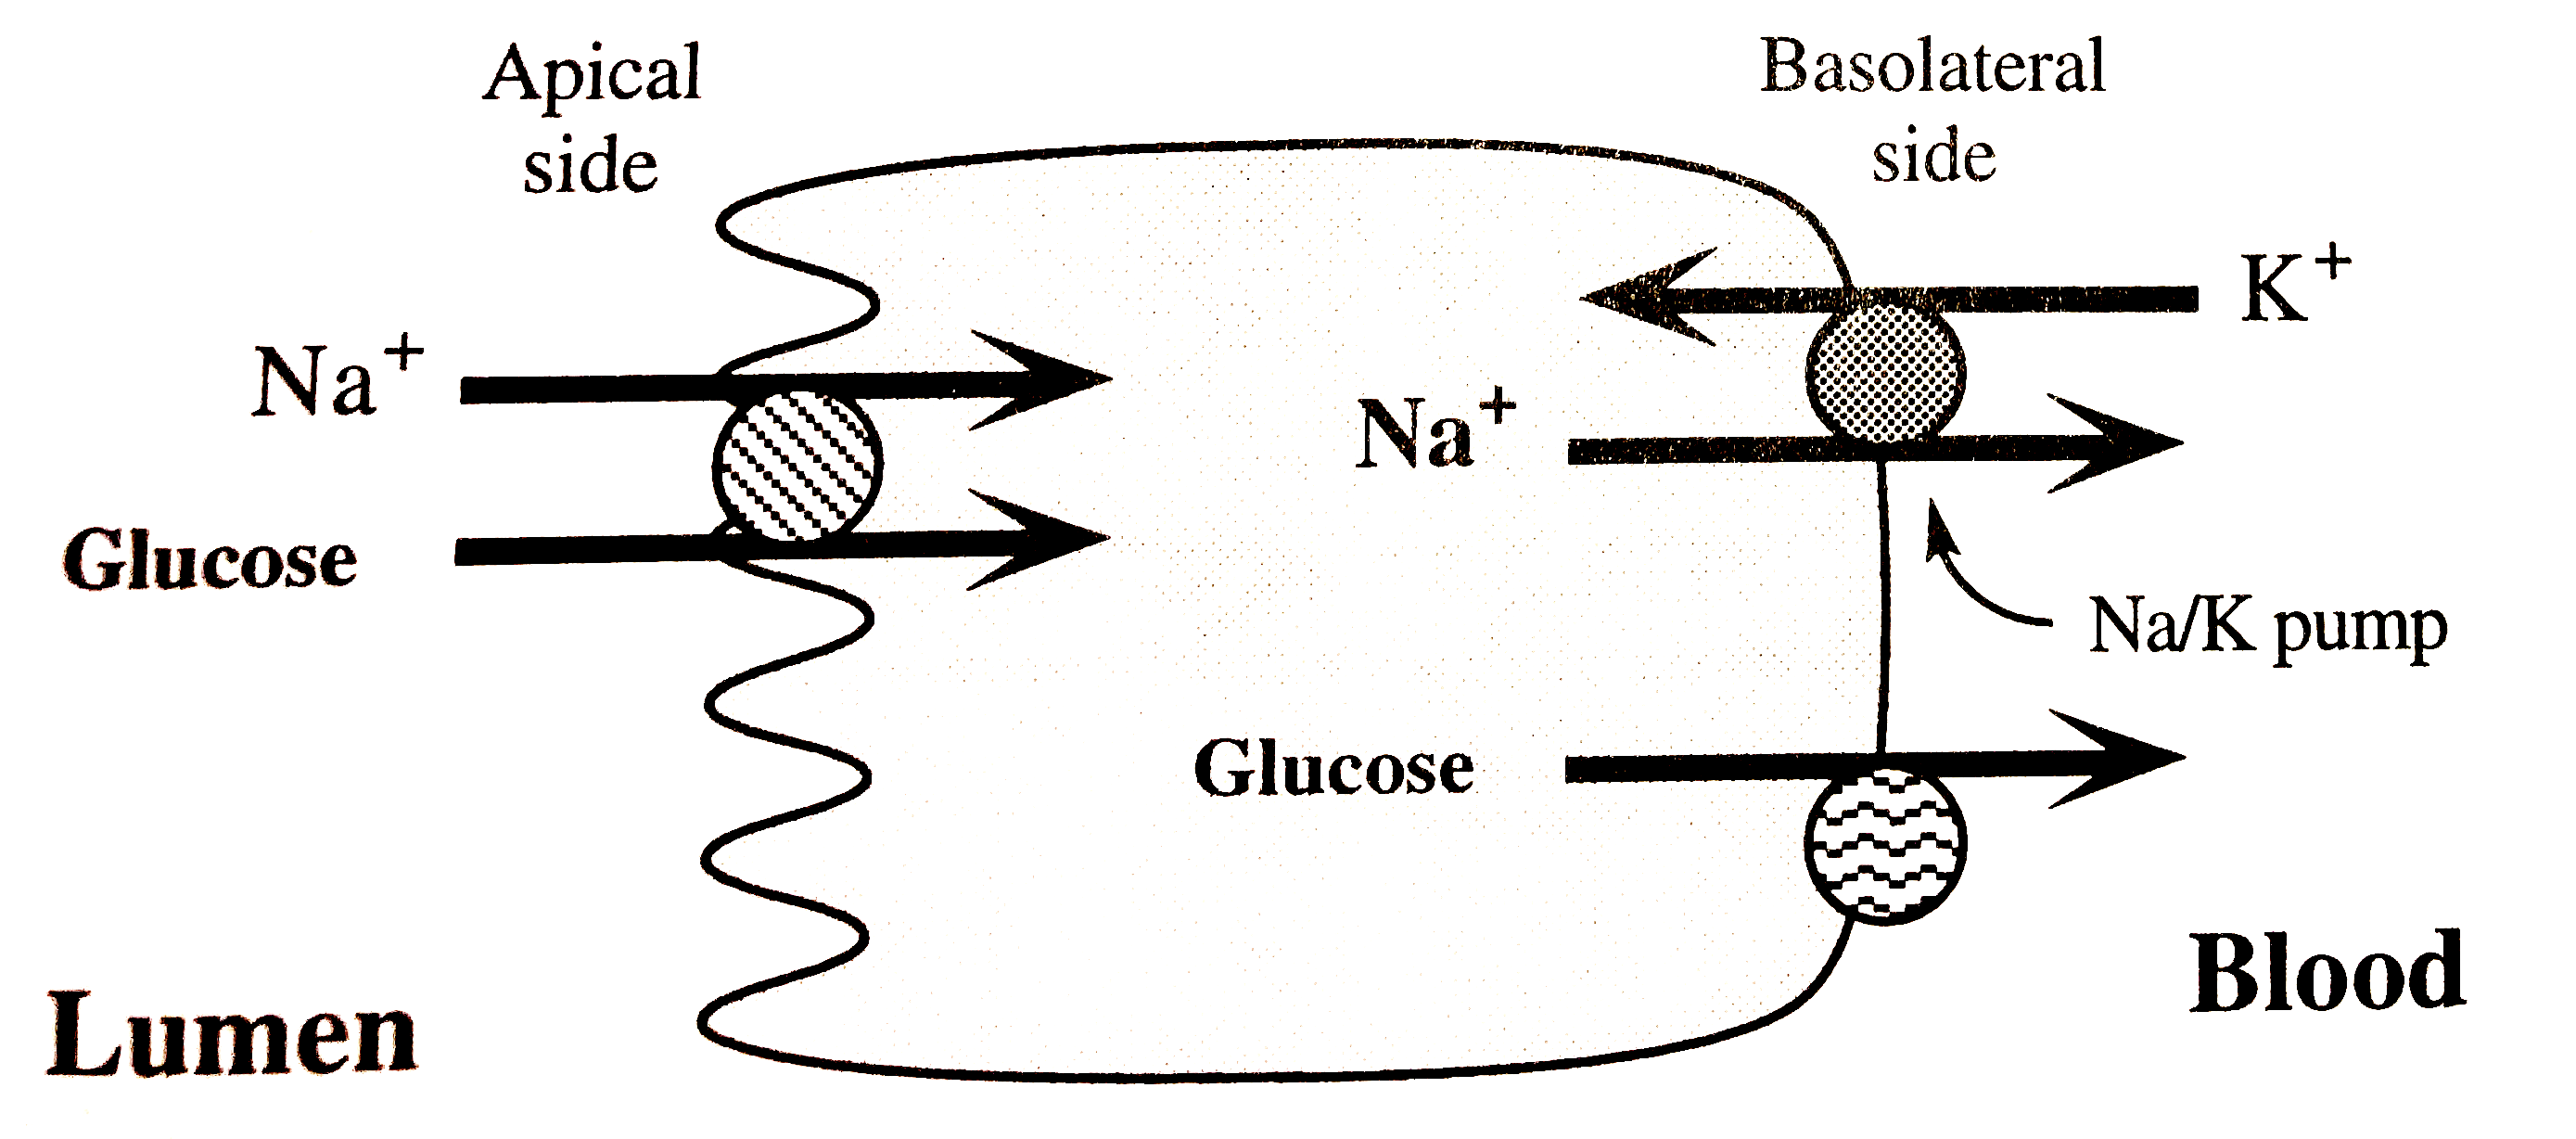
\includegraphics[width=0.7\textwidth]{transport_systems.png} \label{transport_systems}
\caption{Transport systems.}
\end{figure}
\indent Recall that fats are degraded to fatty acids and glycerol by the lipase enzyme. These compounds can diffuse into the intestinal epithelial cells where they are resynthesized into triglycerides (fats) and aggregate into structures called \textbf{chylomicrons}. These aggregates are released at the basolateral membrane and into the extracellular space, and enter the lymph and are transported to the veins and eventually the tissues.\\
\indent The large intestine absorbs most of the water and ions that are left in the chyme as it passes from the small intestine. As the sodium and chloride ions are absorbed, an osmotic gradient is established that allows for the absorption of water. What is not absorbed is passed out of the body in the feces.

\subsection{The Kidney}
Water can be lost from the \textbf{integument} (i.e. the skin) by evaporation, the GI tract, the lungs, and the urinary system. Recall that osmolarity refers to the total solute concentration of a solution. Remember, the higher the osmolarity of a given solution, the lower will be the concentration of water in that solution.\\
\indent If an organism can change the internal ionic concentration of its fluids to meet that of the surrounding environment are referred to as \textbf{osmoconformers}; many marine invertebrates are osmoconformers. However, most vertebrates do not change the internal ionic concentration of their body fluids to meet that of a surrounding environment. Organisms like this are referred to as \textbf{osmoregulators}. \\
\indent Kidneys have three main functions: filtration, reabsorption, and excretion.
\begin{enumerate}
	\item \textbf{Filtration:} The functional unit in the kidney is the \textbf{nephron} which consists of a \textbf{glomerulus}, \textbf{Bowman's capsule}, and a \textbf{tubular} system. The glomerulus is a collection of capillaries that receives blood from an artery terminating in the renal system. Blood is pumped into the glomerulus by the hydrostatic pressure of the heart, and that pressure forces the blood through the capillary walls and into Bowman's capsule. The cell-free ultrafiltrate found in Bowman's capsule lacks many of the plasma proteins found in the blood. Blood \textbf{plasma} is simply a solution which is about $90\%$ water that is composed of organic (i.e. proteins, sugars, amino acids, etc.) and inorganic substances (i.e. various ions like sodium and chloride). There's also erythrocytes, lymphocytes, and platelets. The \textbf{filtrate} in Bowman's capsule is essentially the plasma minus the large MW proteins.
	\item \textbf{Reabsorption:} The kidney also reabsorbs important organic and inorganic compounds from the filtrate in Bowman's capsule. Reabsorption occurs through many of the epithelial cells which line the tubular lumen of the nephron. The \textbf{cilia} of these epithelial cells move in such a way as to help propel the filtrate through these renal tubes. Glucose, small proteins, amino acids, salts, bicarbonate ions, and water are reabsorbed along this tubular system and transported back into the blood. This epithelial cells also have the ability to secrete protons, potassium, urea, uric acid, and ammonia.
	\item \textbf{Excretion:} The kidney also helps excrete waste, salts, and excess water. 
\end{enumerate}
\noindent Blood from the descending aorta enters into the \textbf{renal artery} and eventually into the \textbf{glomeruli} of the nephrons. Blood leaves the kidney by way of the \textbf{renal vein} which itself empties into the inferior vena cava. Leaving each kidney is a \textbf{ureter} which transports the urine to the \textbf{bladder}. Urine exits the bladder by way of the \textbf{urethra}. Each kidney contains more than a million nephrons. The glomerulus and Bowman's capsule of each nephron is located in the \textbf{cortex} and gives this portion of the kidney a \textbf{granular} appeareance. In contrast, the \textbf{striated} appearance of the \textbf{medulla} is primarily due to a portion of the system of the nephron called the \textbf{loop of Henle} and the \textbf{collecting duct}. The collecting ducts, which collect the urine, empty into the renal pelvis of the kidney and then into the ureter. \\
\indent The functional unit of the kidney is the \textbf{nephron}. As the \textbf{renal artery} branches into smaller division and enters the kidney, it becomes the \textbf{afferent arteriole}, which then enters into the \textbf{Bowman's capsule} and forms the capillary bed called the \textbf{glomerulus}. An \textbf{efferent arteriole} leaves the glomerulus and forms a capillary network which surround the renal tubules. The blood that leaves this capillary network does so by a \textbf{venule} which later empties into the \textbf{renal vein} that leaves the kidney. Extending from Bowman's capsule is a long tubular structure divided into the \textbf{proximal convoluted tubule (PCT)}, \textbf{loop of Henle}, \textbf{distal convoluted tubule (DCT)}, and the \textbf{collecting duct}. Many different nephrons can attach to a single collecting duct. The anatomy of the nephron is shown in \textbf{Fig. \ref{nephron}}.\\
\begin{figure}[!ht]
\centering
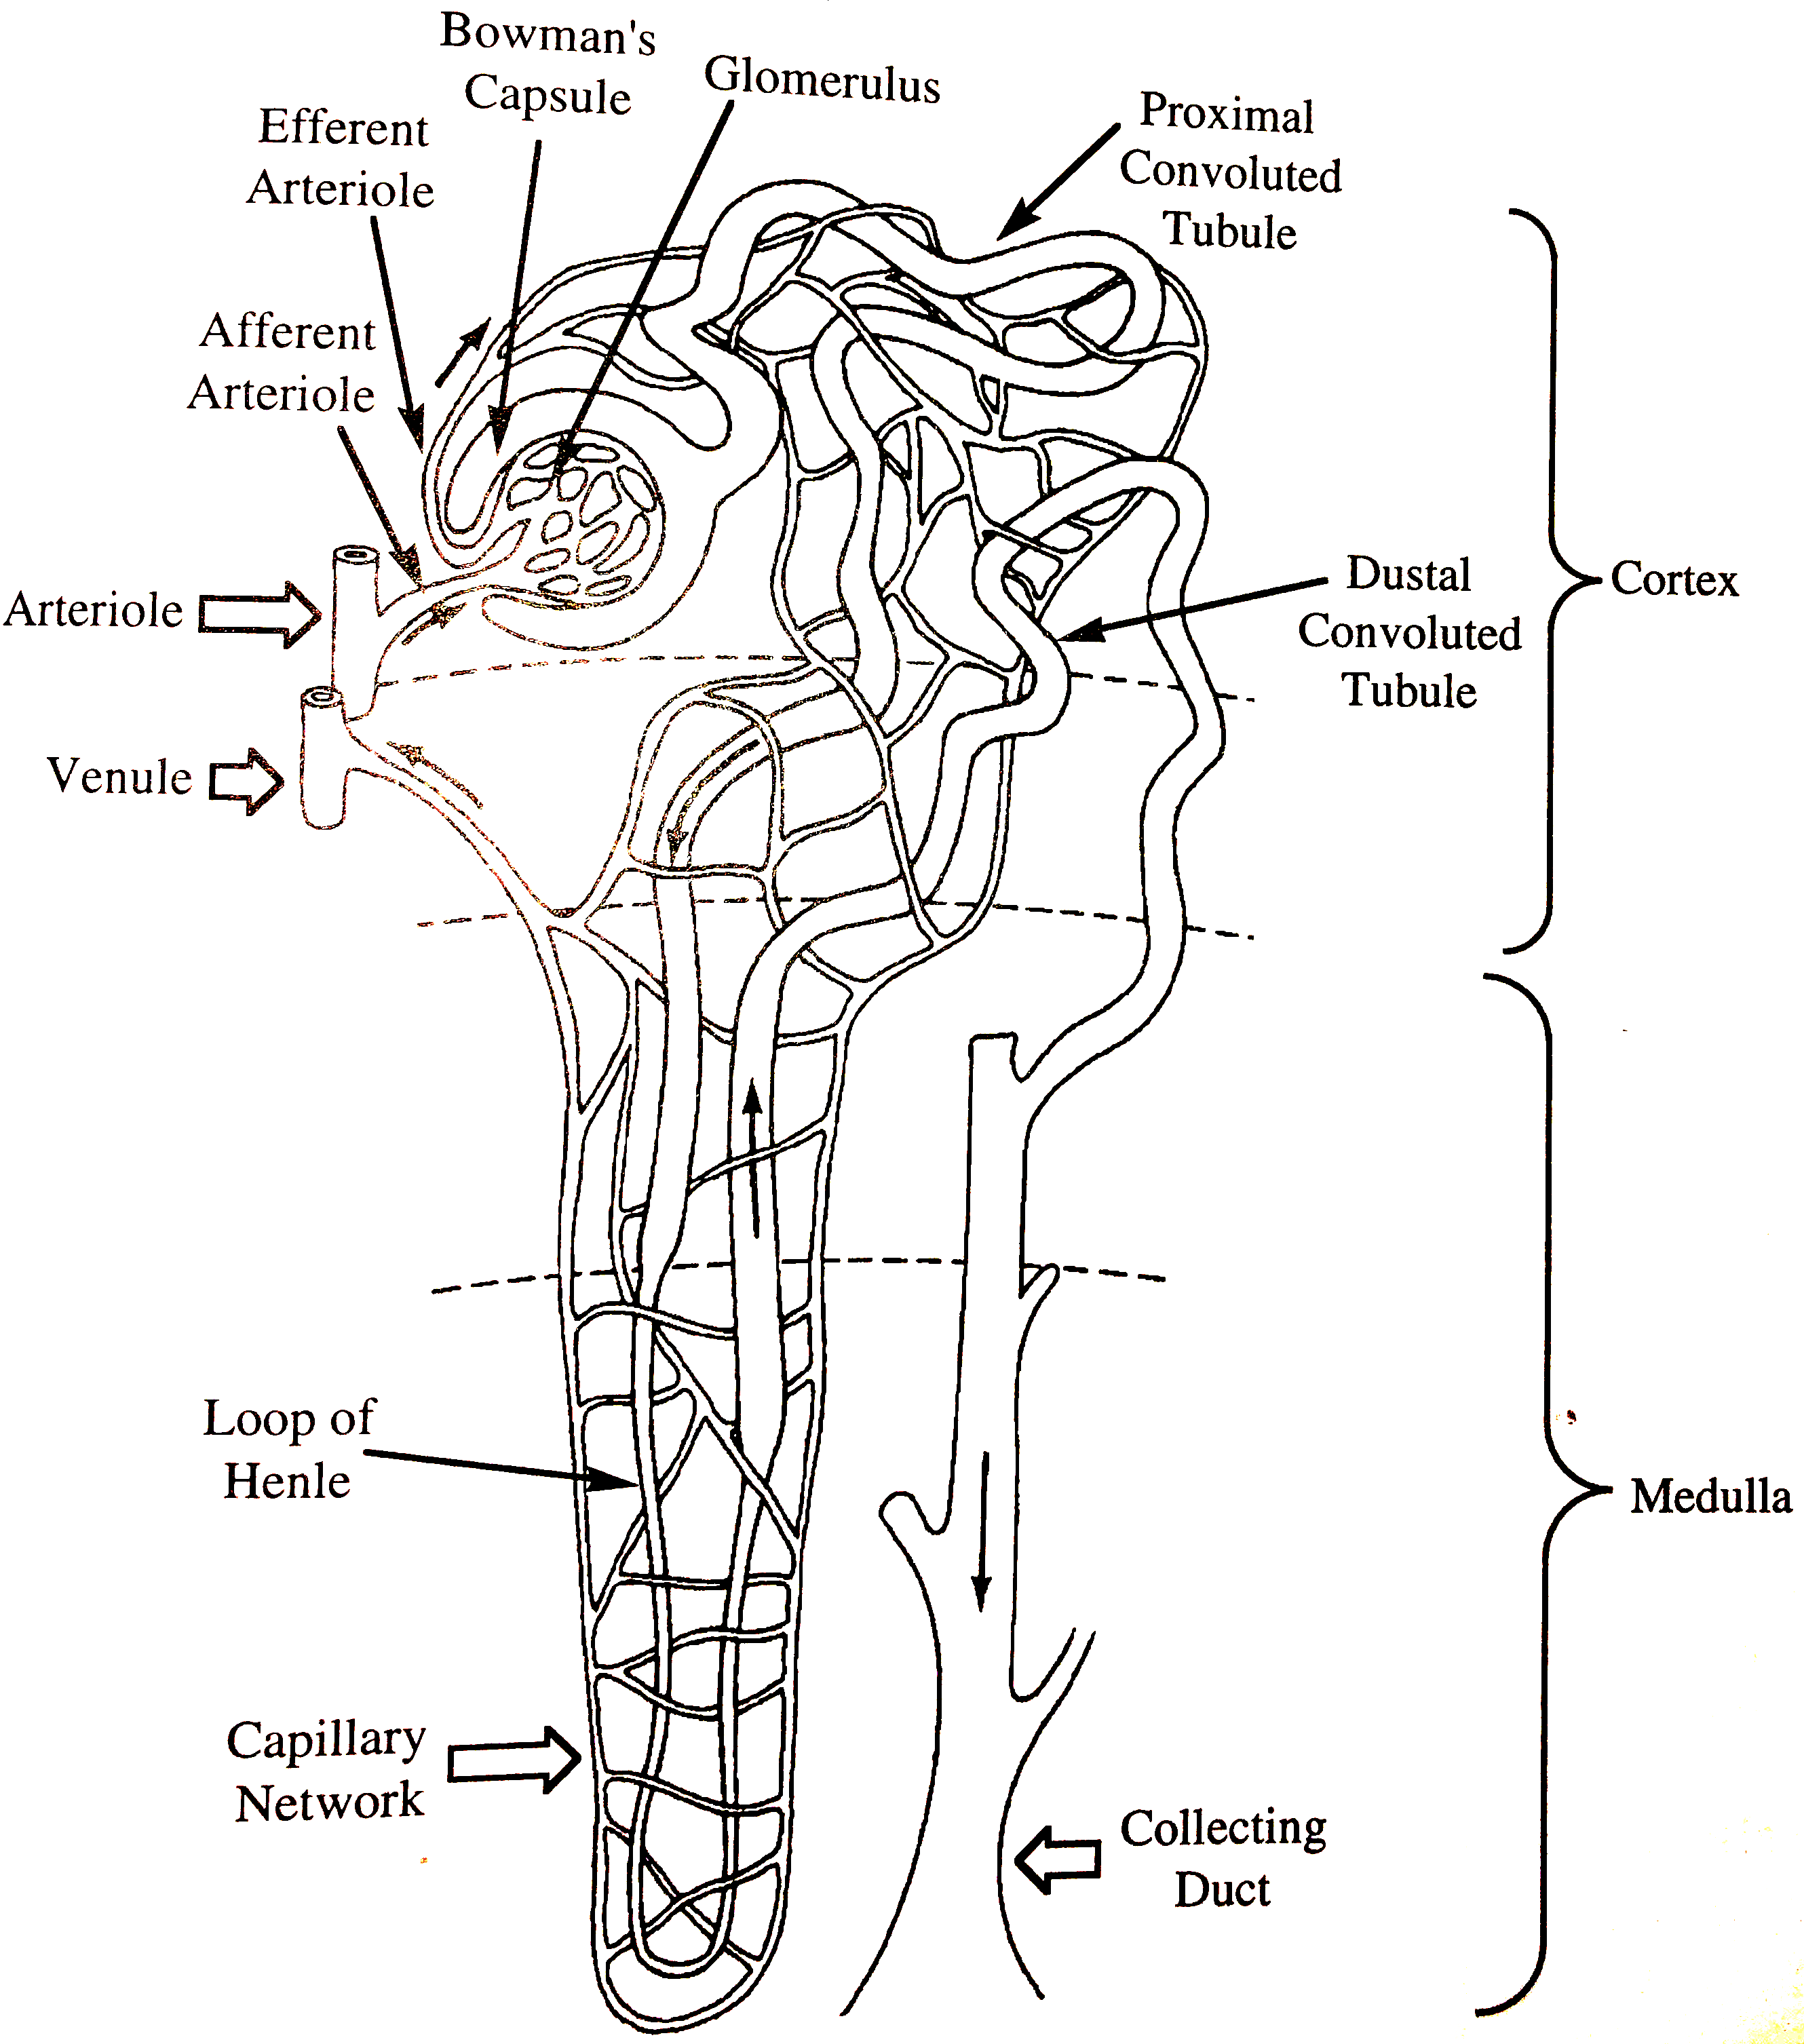
\includegraphics[width=0.7\textwidth]{nephron.png} \label{nephron}
\caption{The nephron and its related capillary system.}
\end{figure}
\indent The PCT is the \textit{obligatory} section of the nephron because roughly $65\%$ of all reabsorption and secretion occurs here. Little regulation occurs in the PCT. Glucose, small MW proteins, amino acids, and vitamins are \textit{completely} reabsorbed in the PCT, and roughly $80\%$ of \ce{Na+}, \ce{Cl-}, and water are reabsorbed in the PCT. As the PCT begins to descend from the cortex into the medulla, it forms the loop of Henle, which has a thin portion and thick portion. The descending thin portion is very permeable to water but only relatively permeable to ions and molecules. The ascending thin portion is the reverse. As the loop of Henle ascends it becomes thicker. The epithelial cells in this region actively transport ions like \ce{Na+} and \ce{K+} from the lumen of the loop into the interstitial fluid. However, this region is impermeable to urea and water. The filtrate from the thick portion of the loop of Henle passes into the DCT, which is also impermeable to urea and water but rather permeable to ions. The filtrate becomes even more dilute. The DCT epithelial cells and the collecting duct cells located in the cortical region of the kidney are quite sensitive to \textbf{aldosterone} secreted by the adrenal glands. An increase in aldosterone causes sodium to be reabsorbed by the epithelial cells. These cells also respond to \textbf{antidiuretic hormone (ADH)}, produced by the hypothalamus and released by the posterior pituitary. If the concentration of ADH increases, then water will be reabsorbed from the epithelial cells in the collecting duct and passed to the interstitial space. The cells of the collecting duct can also secrete hydrogen ions (as can the cells of the PCT and DCT).\\
\indent The osmolarity of the filtrate in Bowman's capsule is essentially the same osmolarity in the plasma. 

\subsection{Homeostatic Mechanisms}
Suppose we want to maintain the levels of sodium in the body. Certain cells in the cortex of the adrenal gland are sensitive to the levels of sodium in the blood. When the concentration of \ce{Na+} \textit{decreases} in the blood, these cells release the hormone \textbf{aldosterone}, which acts at the level of the \textbf{DCT} (distal convoluted tubule) and the \textbf{collecting ducts} and stimulates the epithelial cells in those regions to reabsorb sodium. As a result, the blood concentration of sodium begins to rise. This acts as a signal and feeds back on the cortical cells of the adrenal gland, telling it to reduce the secretion of aldosterone.\\
\indent Suppose we want to maintain the proper levels of water in the body. If there's a \textit{decrease} in the plasma volume of the body, there will be a lower blood pressure (detected by baroreceptors) but a higher osmotic pressure (detected by osmoreceptors). These receptors would stimulate specific cells in the hypothalamus to synthesize and transmit \textbf{ADH} (anti-diuretic hormone) to the posterior pituitary where it is released into the blood. ADH stimulates the epithelial cells in the latter portion of the \textbf{DCT} and collecting ducts to absorb water. This leads to less water excretion and a higher plasma volume. If you were to drink too much water, then the opposite process would happen and you would excrete copious amounts of urine.\\
\indent We also should talk about nitrogenous wastes. Proteins and nucleic acids are the two primary metabolic sources of nitrogenous wastes, and can be removed as ammonia, urea, or uric acid. Ammonia is toxic and soluble, urea is less-toxic and soluble, and uric acid is toxic and insoluble. Fish metabolize glutamine into ammonia, which can be easily carried away with the passing water. Urea is excreted by most mammals, amphibians, and some reptiles and birds. The ammonia that is produced from the metabolism from the amino acids Gly, Asp, and Glu can be converted to uric acid, which is the primary excretory product of birds and reptiles. \\
\indent The normal pH of the body is 7.4. Anything below 7.35 or above 7.45 could be fatal if left for an extended period of time. Blood pH is regulated by a \textbf{buffering system} that involves bicarbonate: \ce{H+ + HCO_3- <-> H_2CO_3 <-> CO_2 + H_2O}.\\
\indent Recall that the cholera toxin is cased by the bacterium \textit{Vibro cholerae} and causes the rapid loss of fluid. According to the buffer system above, the loss of bicarbonate results in a shift of the bicarbonate buffer system to the side of the acid (\ce{H+}). If the volume of enteric fluid that is lost is large enough to overwhelm the ability of the kidney to regulate the proper acid-base levels in the body, \textbf{metabolic acidosis} results. An adult with severe untreated cholera in the blood pH can drop to a more acidic value of 7.19. To try to compensate, a clinical feature of metabolic acidosis is \textbf{hyperventilation} to try to eliminate the increased \ce{CO_2} more quickly, as by lowering the concentration of \ce{CO_2} in the body, the levels of \ce{H+} are also lowered. 

\subsection{Male Reproduction}
From an endocrinology standpoint, we have the following pathway:
\begin{equation}
\begin{split}
\text{Hypothalamus releases GnRH} \rightarrow \text{Anterior Pituitary releases LH and FSH} \rightarrow \text{Gonads produce steroids and germ cells}
\end{split}
\end{equation}
\noindent Note that this general signaling pathway applies to both males and females. \textbf{GnRH} is the \textbf{gonadotropin releasing hormone}, \textbf{LH} is \textbf{luteinizing hormone}, and \textbf{FSH} is follicle stimulating hormone. Both LH and FSH are called \textbf{gonadotropins}. In males, the germ cells ultimately produced are called \textbf{spermatozoa}, while in the female they are the \textbf{ova}. The male reproductive anatomy is shown in \textbf{Fig. \ref{male_reproductive_anatomy}}. 
\begin{figure}[!ht]
\centering
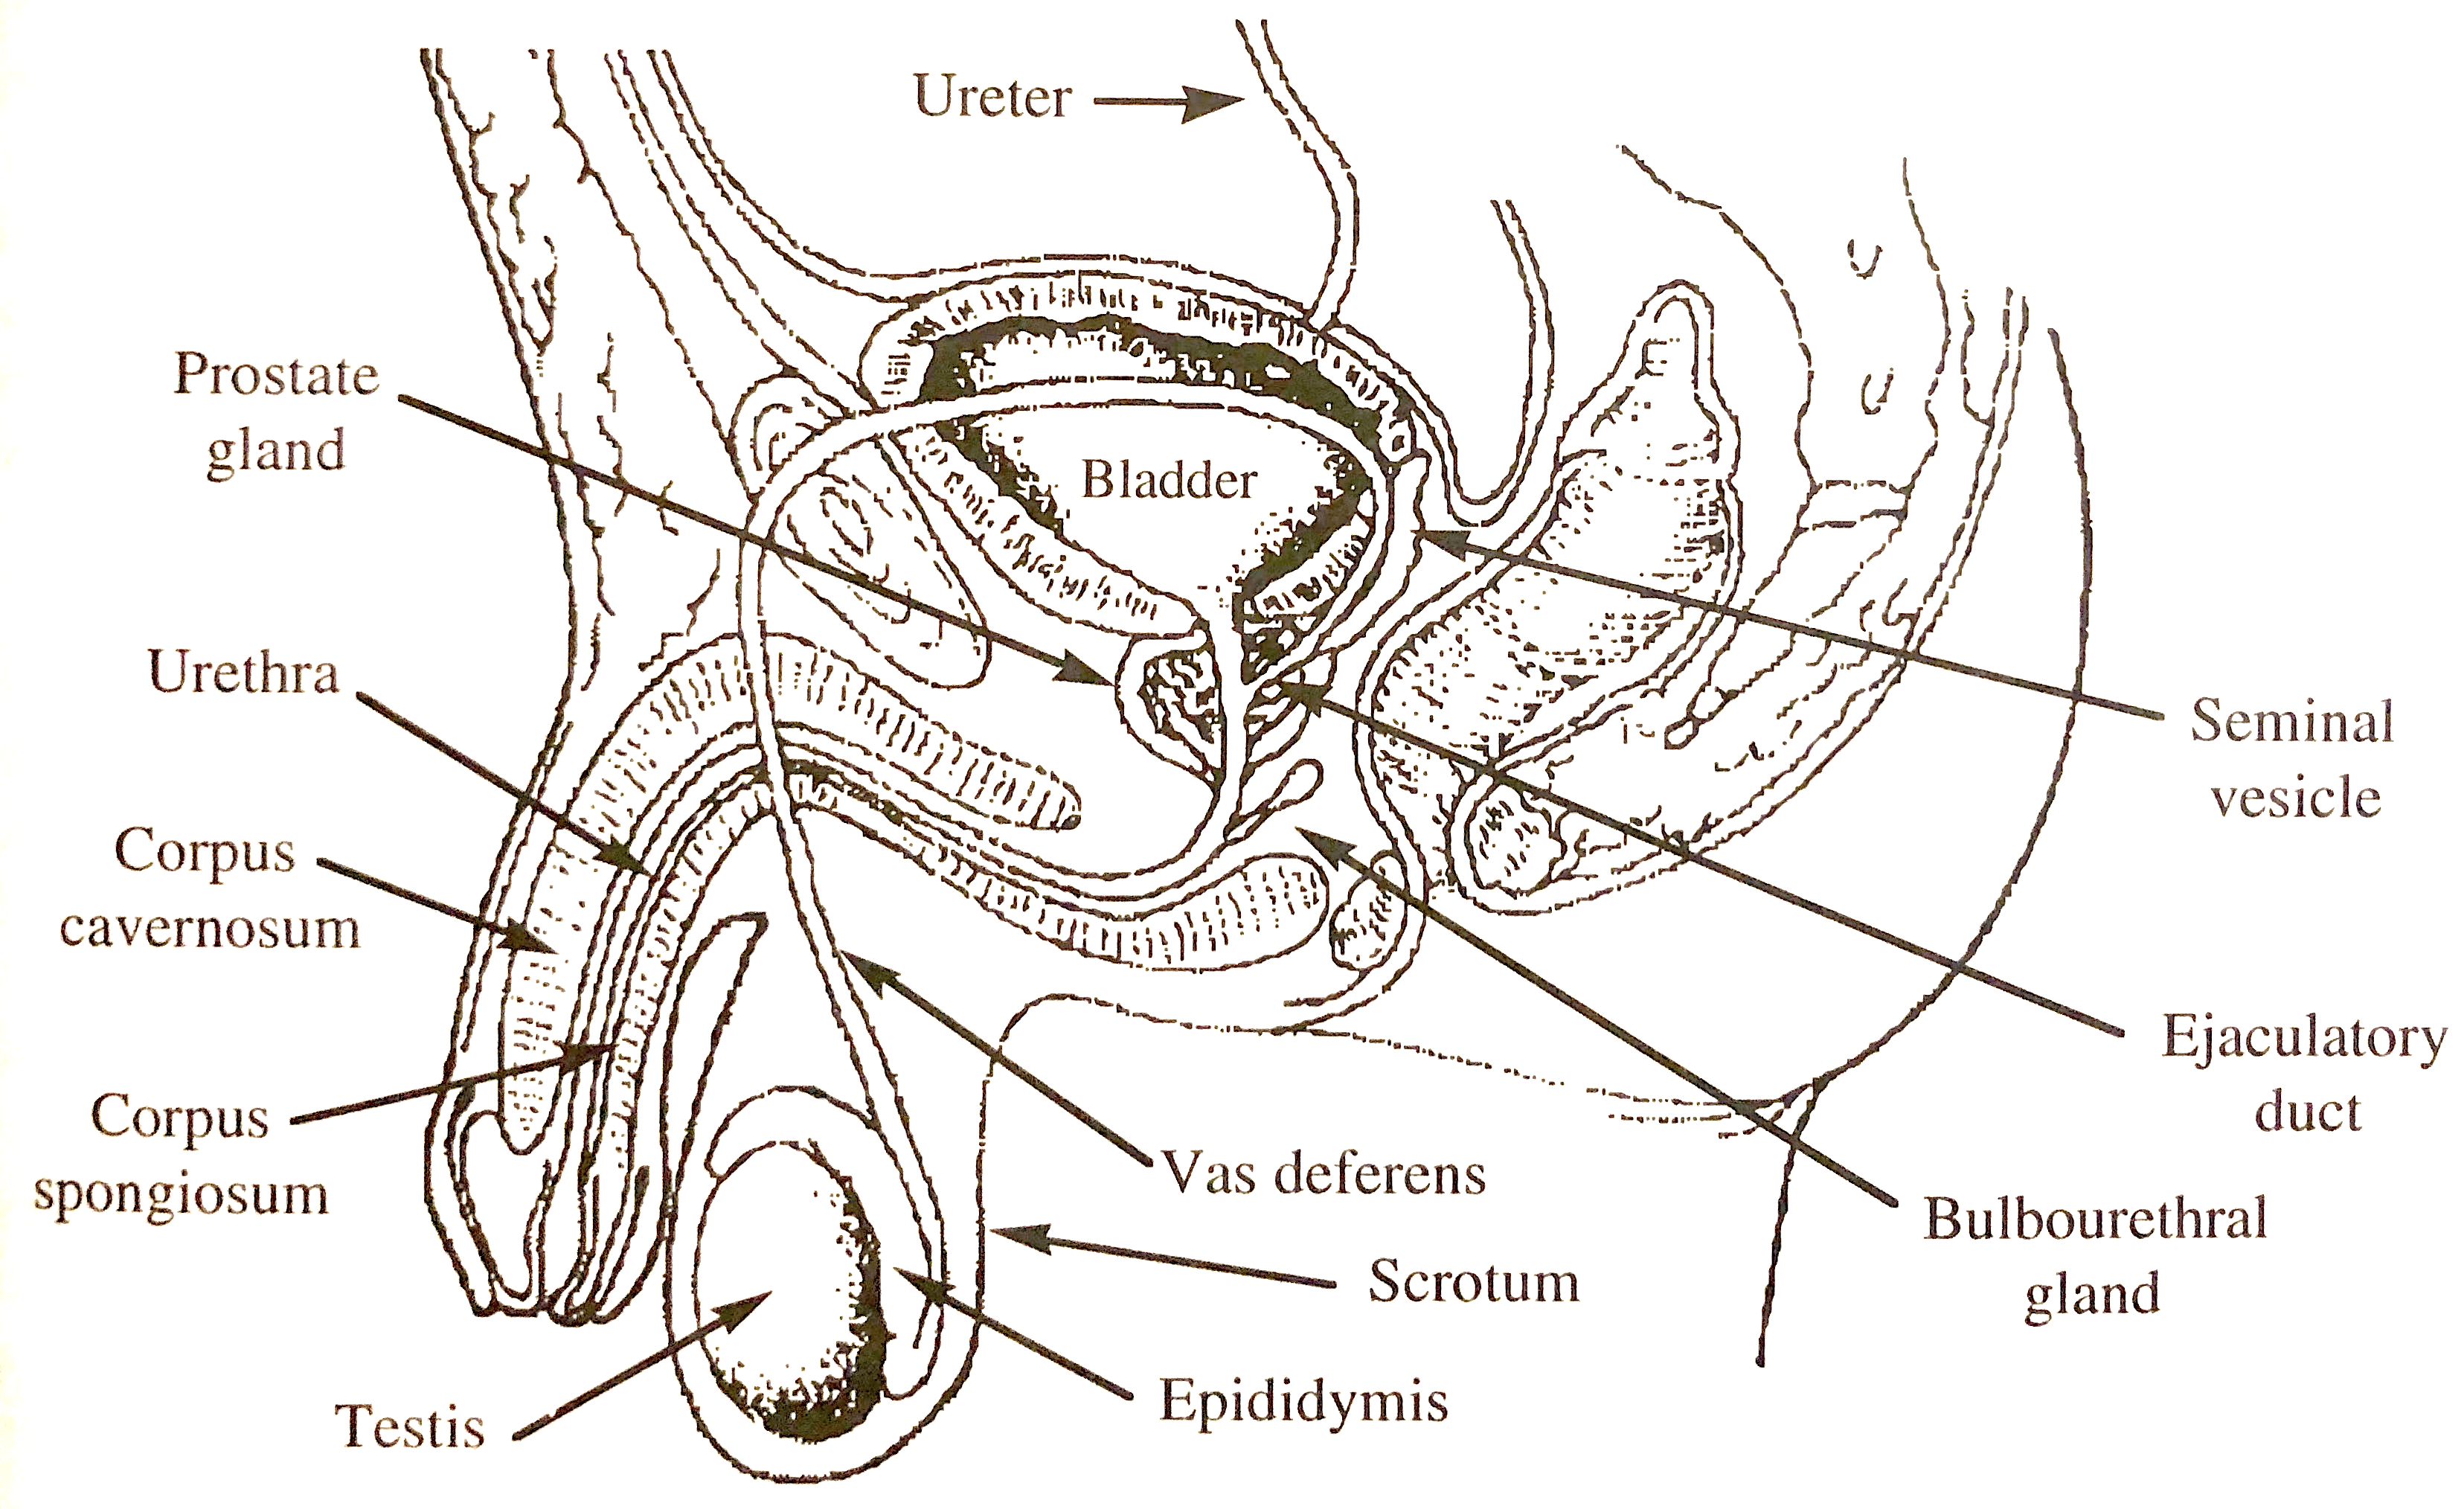
\includegraphics[width=0.7\textwidth]{male_reproductive_anatomy.png} \label{male_reproductive_anatomy}
\caption{Male reproductive anatomy.}
\end{figure}
\noindent Because spermatogenesis requires a lower temperature than that of the body, they are produced in the testes that lie in the scrotum outside the body cavity. Within each testis are a series of convoluted tubules celled the \textbf{seminiferous tubules}, and each of these tubules has the \textbf{spermatogenic cells}. The testes also produce the hormone \textbf{testosterone} using specialized interstitial cells called \textbf{Leydig cells} (also called the \textbf{interstitial cells}) that lie outside the seminiferous tubules. There are also \textbf{Sertoli cells} that lie outside the area of the seminiferous tubule, which promote spermatogenesis and produce the protein hormone \textbf{inhibin}. The Sertoli cells are in direct contact with the spermatogenic cells, and are adjacent to the lumenal space. \\
\indent Usually, the \textbf{spermatogonia} far away from the lumen of the seminiferous tubules will divide via mitosis. However, as they get closer and closer to the lumen, eventually they are referred to as \textbf{primary spermatocytes} and begin to undergo meiosis, thus producing \textbf{secondary spermatocytes} after the first meiotic division and \textbf{spermatids} after the second meiotic division, which now have half as many chromosomes. The spermatids then transform into the \textbf{spermatozoa}, which are released into the lumen.\\
\indent At the very tip of a spermatozoan, there is a structure called the \textbf{acrosome} which contains a lot of digestive enzymes that help the spermatozoa gain access to the interior of the egg once fertilization has taken place. Inside the head of the spermatozoa is a nucleus which contains the DNA. In the midsection are \textbf{mitochondria}, providing energy for the whipping movement of the tail to allow the sperm to swim towards their destination (i.e. the egg). \\
\indent The Leydig cells produce testosterone by converting cholesterol to it. Testosterone can (1) diffuse out of the Leydig cells and move to other target tissues of the body, (2) diffuse into the nearby Sertoli cells, which convert testosterone into \textbf{dihydrotestosterone (dHT)}. dHT diffuses into the nucleus of the Sertoli cell and causes transcription that ultimately affects the spermatogenic cells.\\
\indent LH (luteinizing hormone) binds to a specific receptor on the membrane of the Leydig cell, and causes the increase of the conversion of cholesterol into testosterone. Meanwhile, FSH (follicle stimulating hormone) binds to a surface receptor on the Sertoli cell that causes (1) an increase in the conversion of testosterone into dHT and (2) an increase in the synthesis of these FSH-sensitive receptors.\\
\indent Testosterone has a \textit{negative} feedback at the anterior pituitary and the hypothalamus, so it's important that it's able to diffuse out of the Leydig cells and enter the bloodstream. Specifically, it prevents the synthesis of GnRH and LH. Meanwhile, the Sertoli cells secrete a protein hormone called \textbf{inhibin}, which acts as a negative modulator of the anterior pituitary. Thus, if testosterone levels are too high, the feedback mechanism will decrease the levels of LH. If the levels of dHT are too high, there is an increase in inhibin synthesis that results in the decrease in FSH levels.\\
\indent Almost all of the secondary sex characteristics in the male are due to testosterone. After sperm is produced, they leave the seminiferous tubules and entire into the \textbf{epididymis} and then the \textbf{vas deferens}. Sperm is stored in these regions for about 14 days before ejaculation. Contraction of smooth muscle lining the walls of these structures ejects the sperm down the vas deferens and into the \textbf{ejaculatory duct}. The \textbf{seminal vesicles}, \textbf{prostate gland}, and \textbf{bulbourethral gland} secrete components that make the remainder of the fluid that is ejaculated (now called \textbf{semen}). Some of the components secreted by these glands are fructose vitamins, bicarbonate zinc, prostaglandins, and mucus. Overall, \textbf{Fig. \ref{testes_hormones}} shows us the general hormone involvement in the regulation of testes function.
\begin{figure}[!ht]
\centering
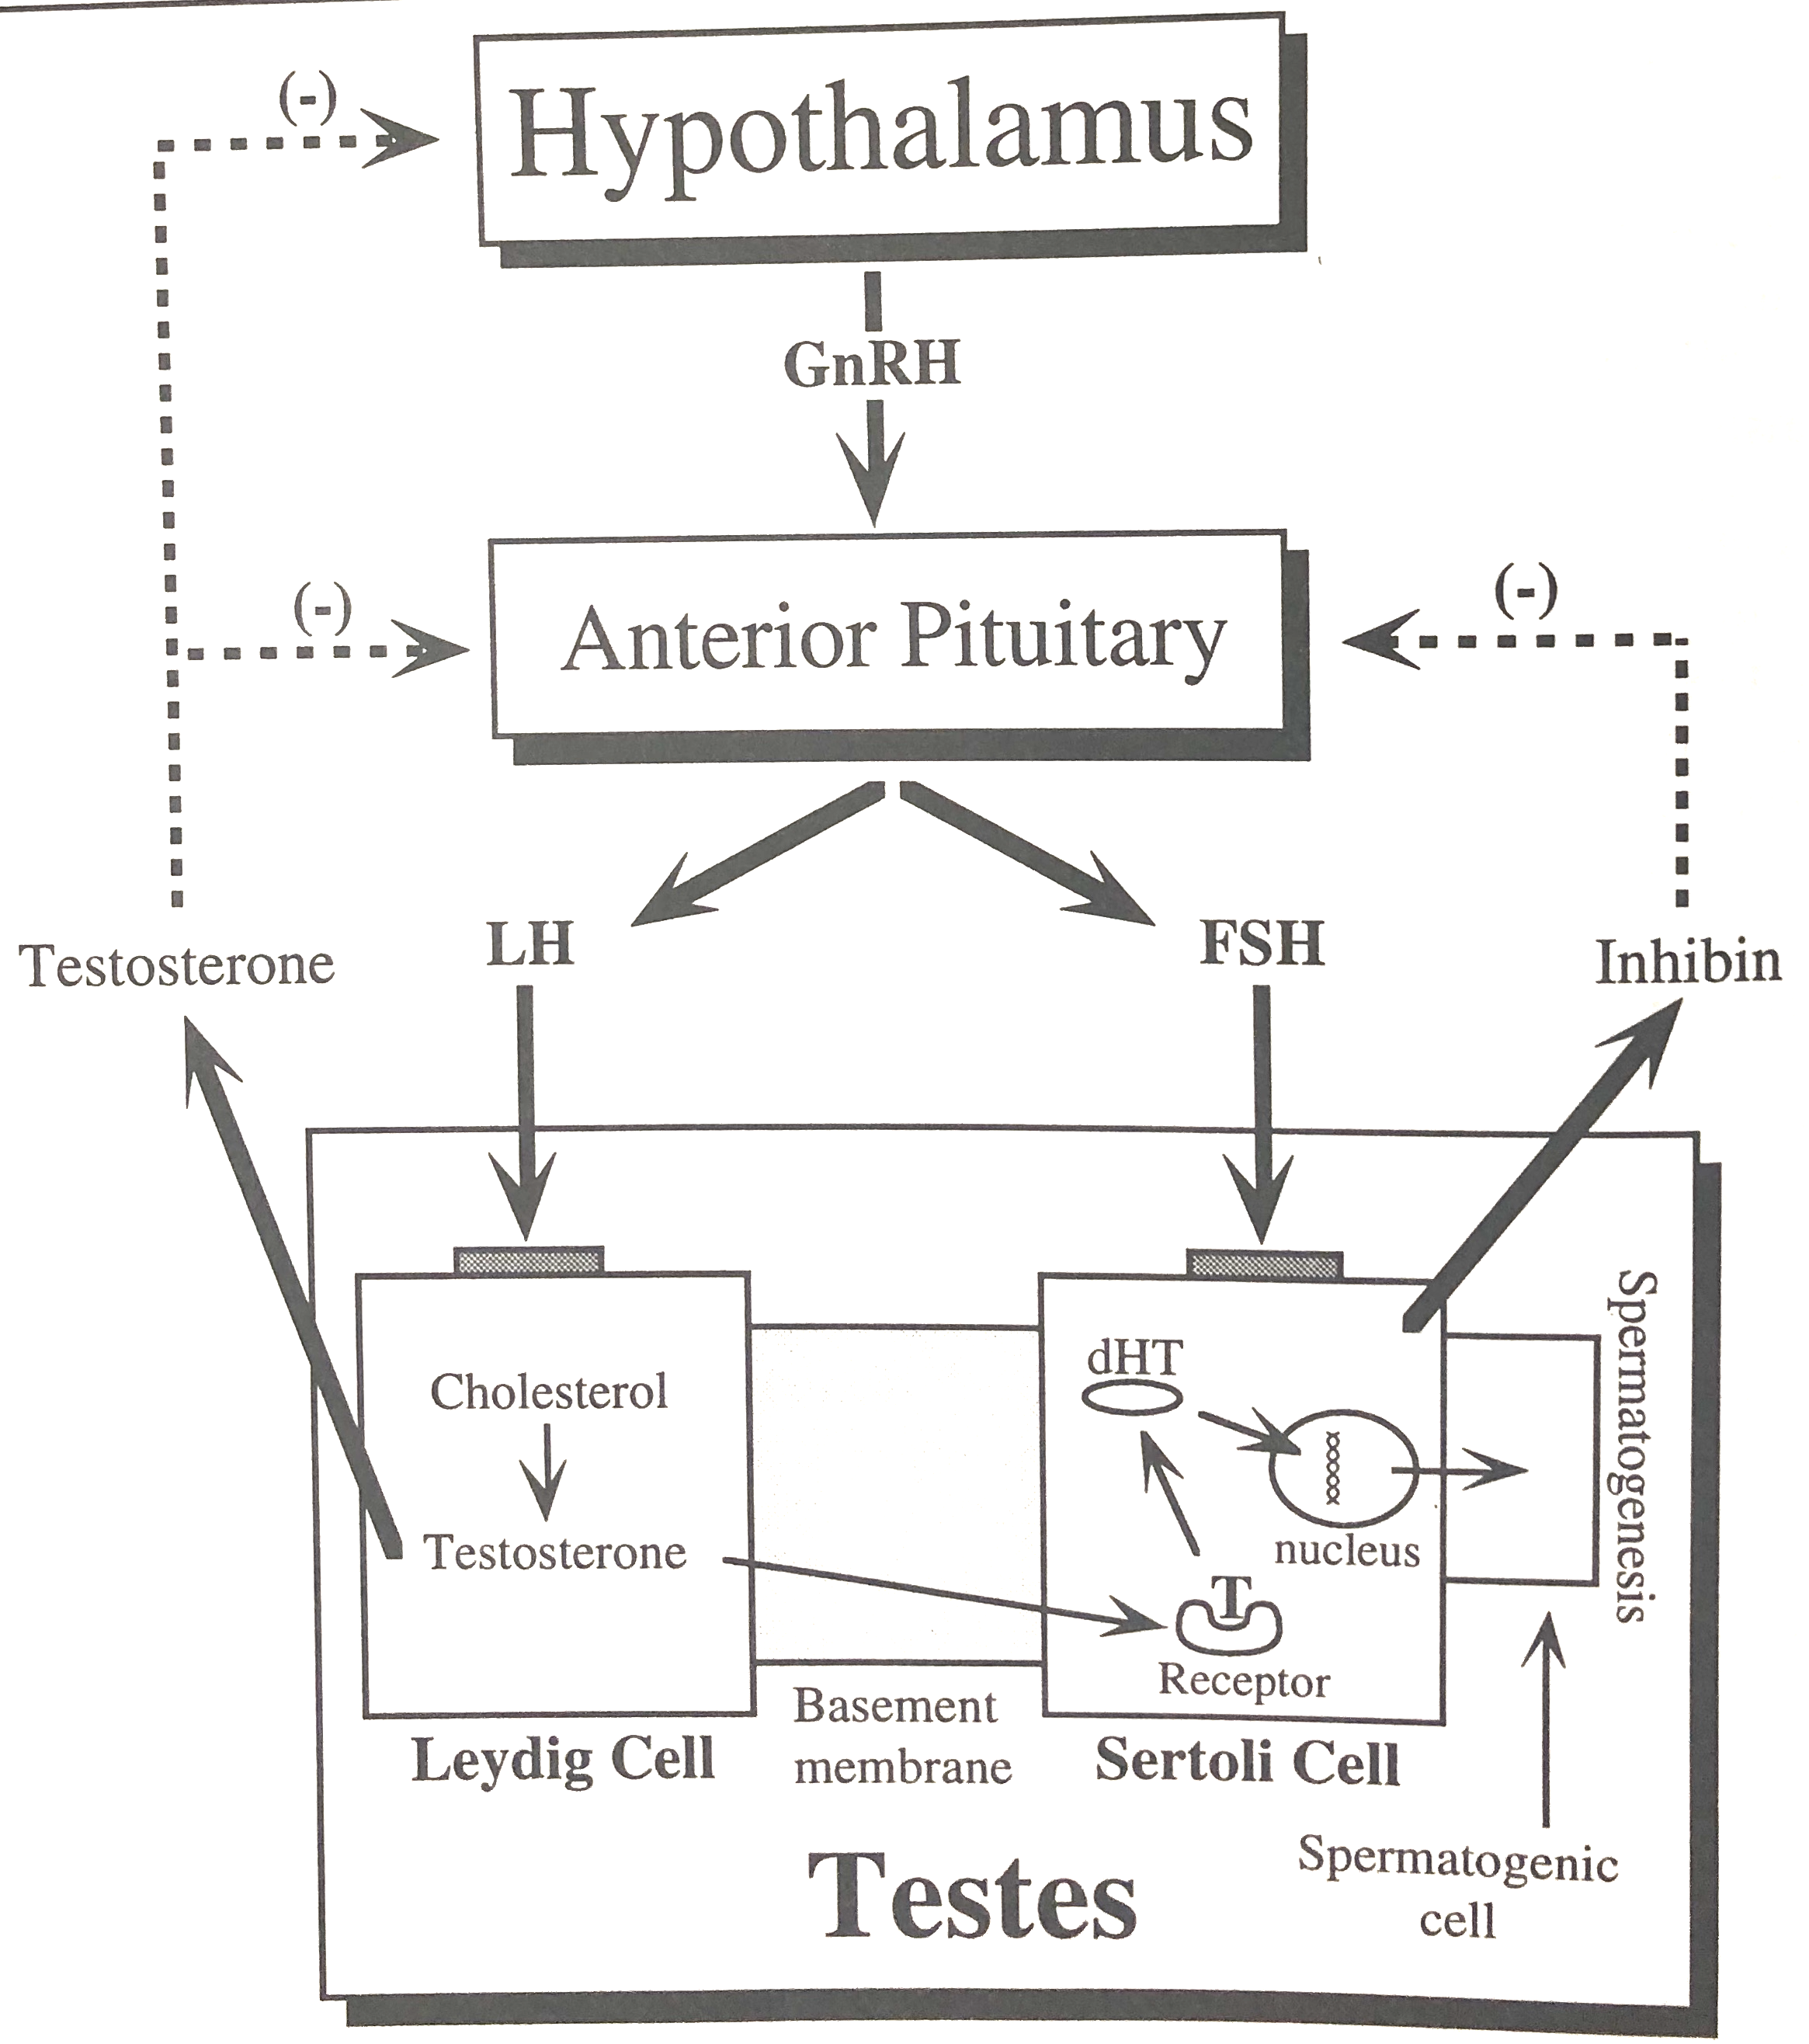
\includegraphics[width=0.5\textwidth]{testes_hormones.png} \label{testes_hormones}
\caption{Hormonal regulation in the testes.}
\end{figure}

\subsection{Female Reproduction}
Once sperm have been ejaculated into the vagina, they can live for about 48 hours. About half an hour after ejaculation, the leading sperm arrive at the \textbf{Fallopian tubes} (also called the \textbf{oviduct}), which is typically the site of fertilization. The fertilized egg continues to move down the oviduct towards the uterus, where it will implant in the uterine lining. About a week after ovulation the fertilized egg, now called a \textbf{blastocyst}, implants in the lining of the uterus where it will continue to grow and develop until \textbf{parturition} (delivery). The general female reproductive anatomy is shown in \textbf{Fig. \ref{female_reproductive_anatomy}}.
\begin{figure}[!ht]
\centering
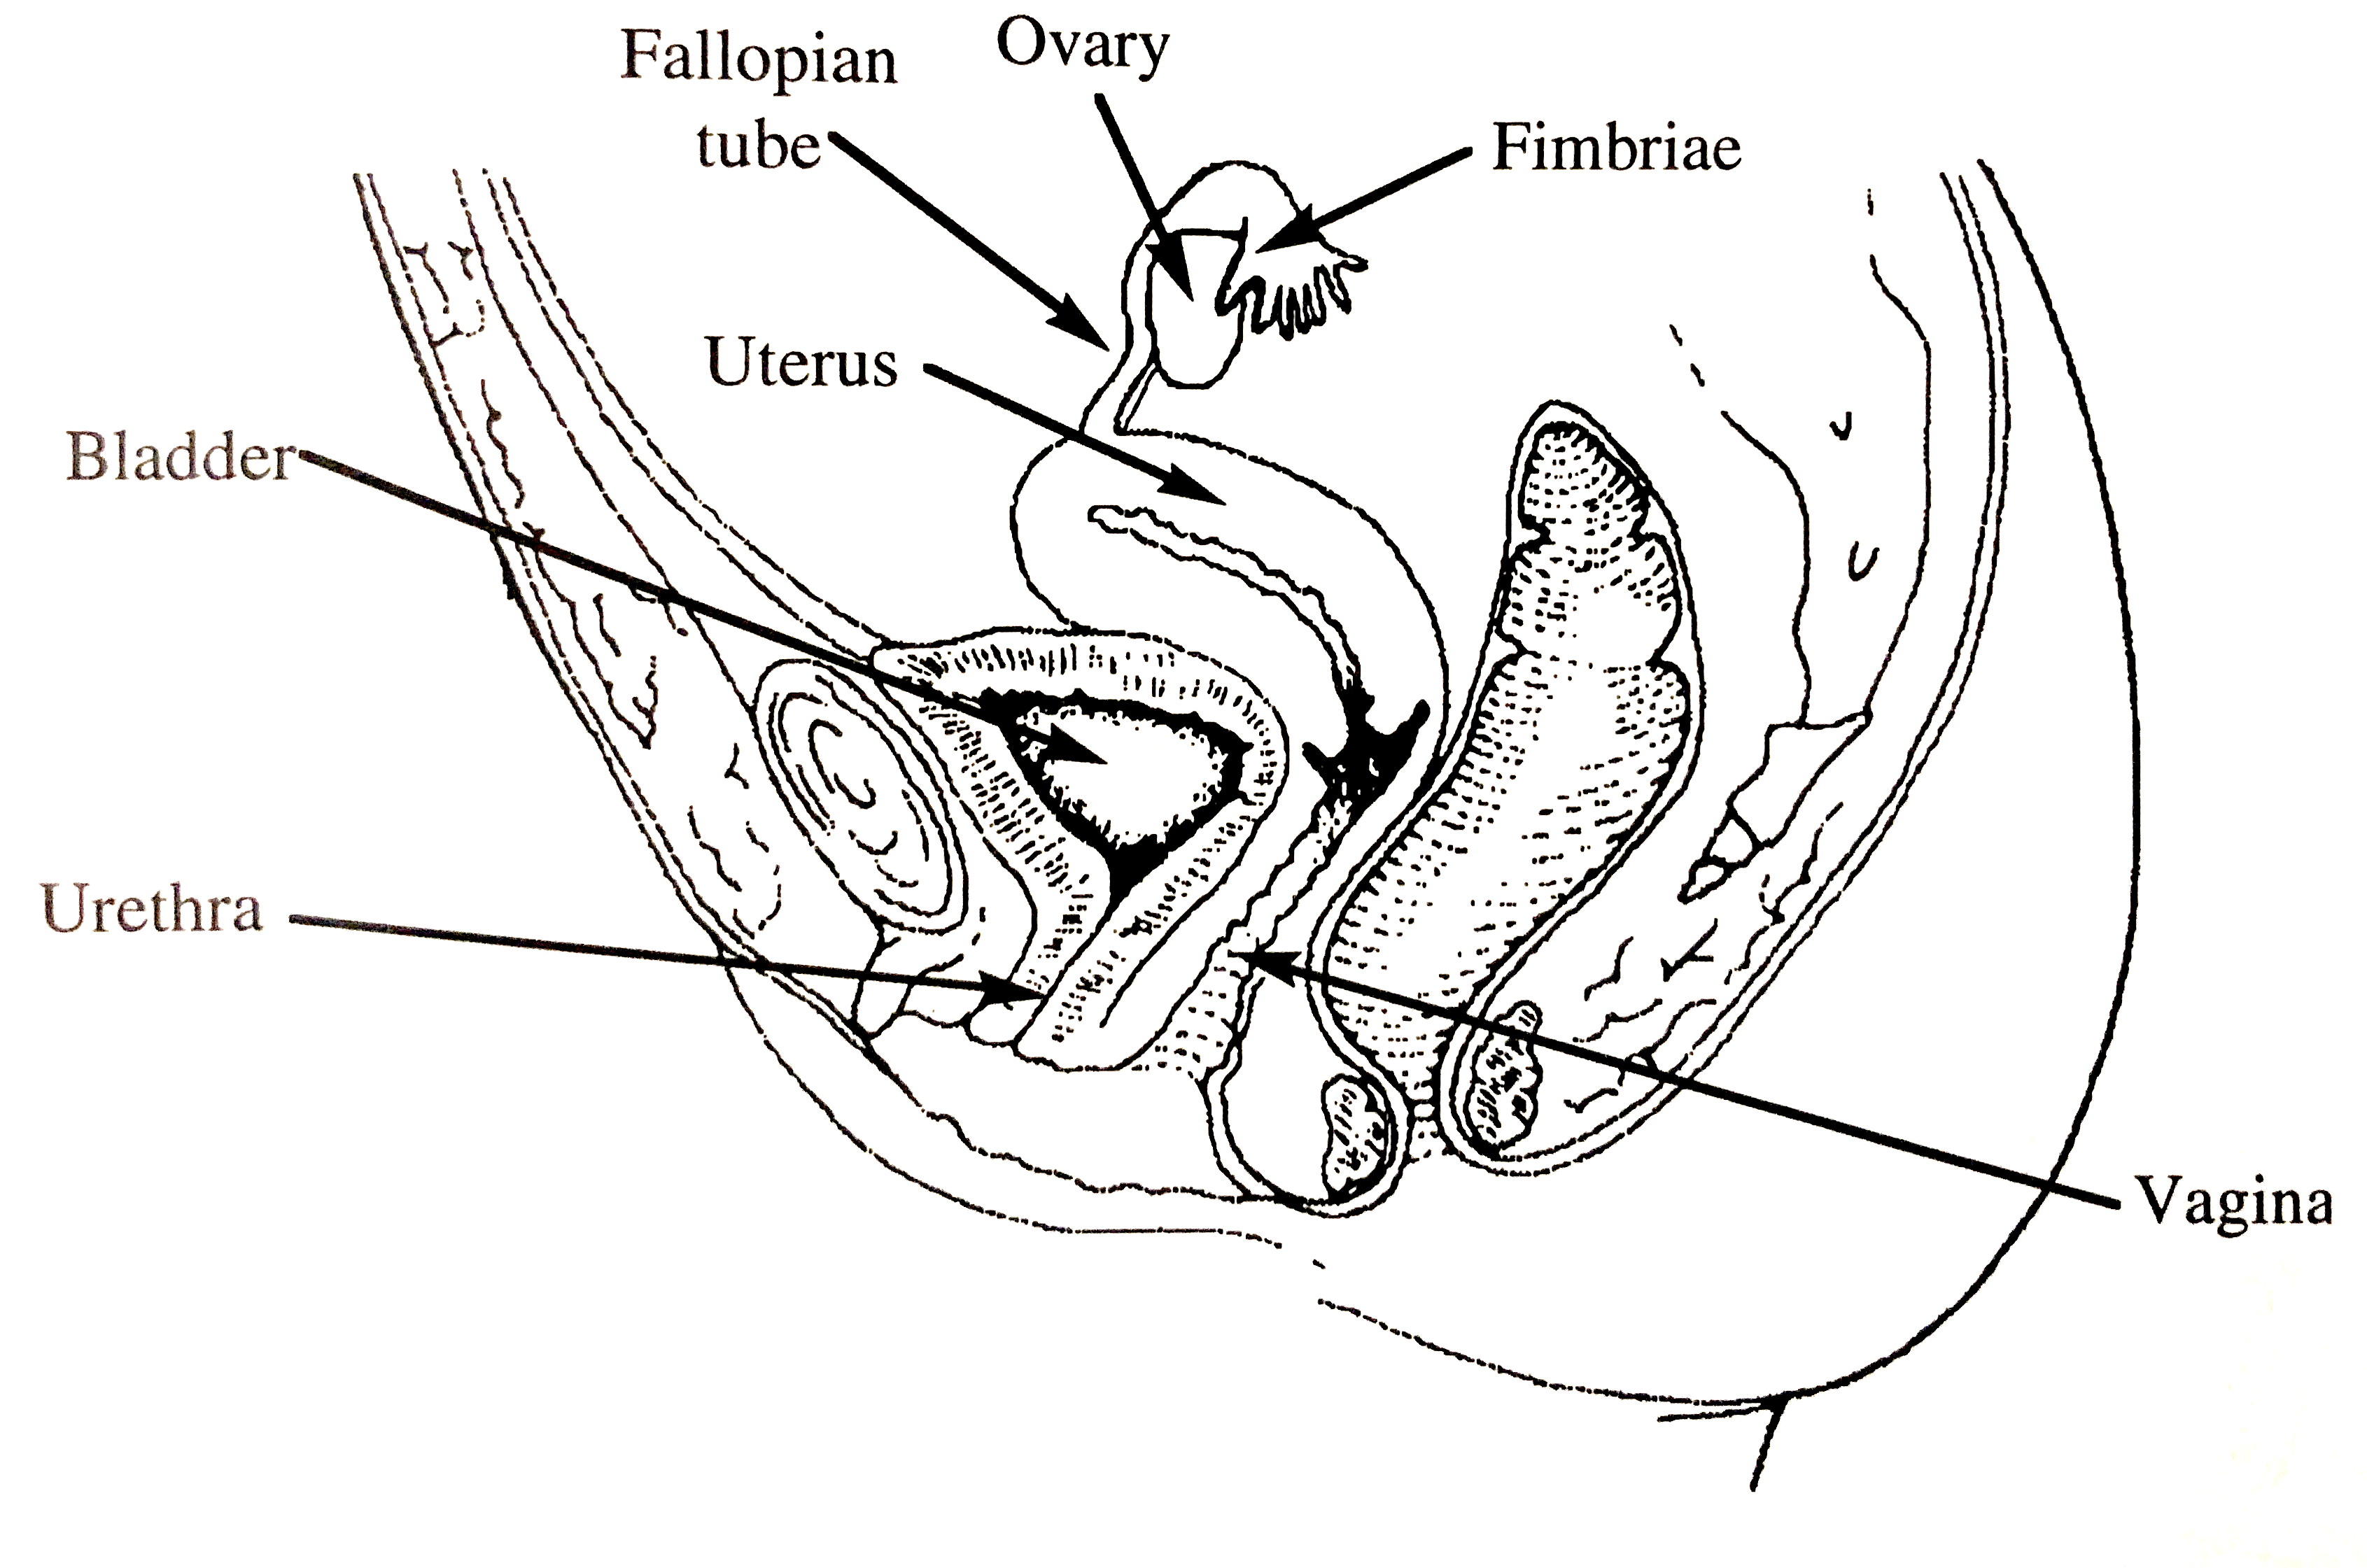
\includegraphics[width=0.7\textwidth]{female_reproductive_anatomy.png} \label{female_reproductive_anatomy}
\caption{Female reproductive anatomy.}
\end{figure}
\noindent The production of female germ cells is called \textbf{oogenesis}. First, oogonia mitotically divide to form \textbf{primary oocytes}. All of these divisions to form primary oocytes occur in the first \textit{two to three months of fetal development}. At birth a female will have about 400,000 primary oocytes, but by the time she has finished her reproductive life only about 400 will have ever matured. The remaining primary oocytes will have degenerated at various stages during the developmental process\textemdash the process of degeneration is called \textbf{atresia}.\\
\indent The primary oocytes then undergo the first meiotic division, caused by a surge in the gonadotropin \textbf{LH}, forming the \textbf{secondary oocytes}. This first meiotic division happens in monthly cycles. During this division, one of the two daughter cells obtains all the cytoplasm while the other is just a small sphere of DNA called the \textbf{first polar body}. The secondary oocyte undergoes the second meiotic division \textit{only after fertilization has taken place}. The result of that division is the \textbf{ovum} and a \textbf{second polar body}. The first polar body also divides to give two second polar bodies as well.\\
\indent If we take a cross-section of the ovary, we will see a series of specific cell types called \textbf{primary follicles} that are in different developmental states. The primary follicle is a \textbf{primary oocyte} surrounded by a layer of follicle cells. These follicle cells are in constant contact with the primary oocyte. Eventually, one of the primary follicles will start to develop (two of them if there are fraternal twins). In order to mature the primary oocyte, \textbf{estrogen}, \textbf{LH}, and \textbf{FSH} are needed. This developing time period is referred to as the \textbf{follicular phase} and lasts up to about the 14th day of the woman's monthly cycle. During this period, the primary follicle gradually develops. Surrounding the primary oocyte will be a membrane called the \textbf{zona pellucida}, which itself is surrounded by more follicle cells called \textbf{granulosa cells} and finally by \textbf{theca cells}. These cell types are a direct result of the estrogen, LH, and FSH that are present. The \textbf{theca cells} are analogous to the \textbf{Leydig cells} in the male, while the \textbf{granulosa cells} are analogous to the \textbf{Sertoli cells} in the male.\\
\indent Within the primary follicle, a fluid starts to build up forming the \textbf{antrum}. Next, the \textbf{LH surge} event causes the primary oocyte to undergo the first meiotic division, forming a polar body and secondary oocyte. The LH surge also causes the production of a series of enzymes that break down the membrane in the primary follicle. Once the secondary oocyte is released, \textbf{ovulation} has occurred. Ovulation usually comes at about the 14th day in the woman's monthly cycle. The left over follicle after the completion of the follicular phase is transformed into a gland-like structure called the \textbf{corpus luteum}. One of the main functions of the corpus luteum is to produce \textbf{estrogen} and \textbf{progesterone}. If fertilization does not occur and there is no pregnancy, the corpus luteum will degenerate and the whole cycle starts again. From the point of ovulation, at about the 14th day, until the beginning of the menstrual flow is the \textbf{luteal phase}. See \textbf{Fig. \ref{ovarian_cycle}}.\\
\begin{figure}[!ht]
\centering
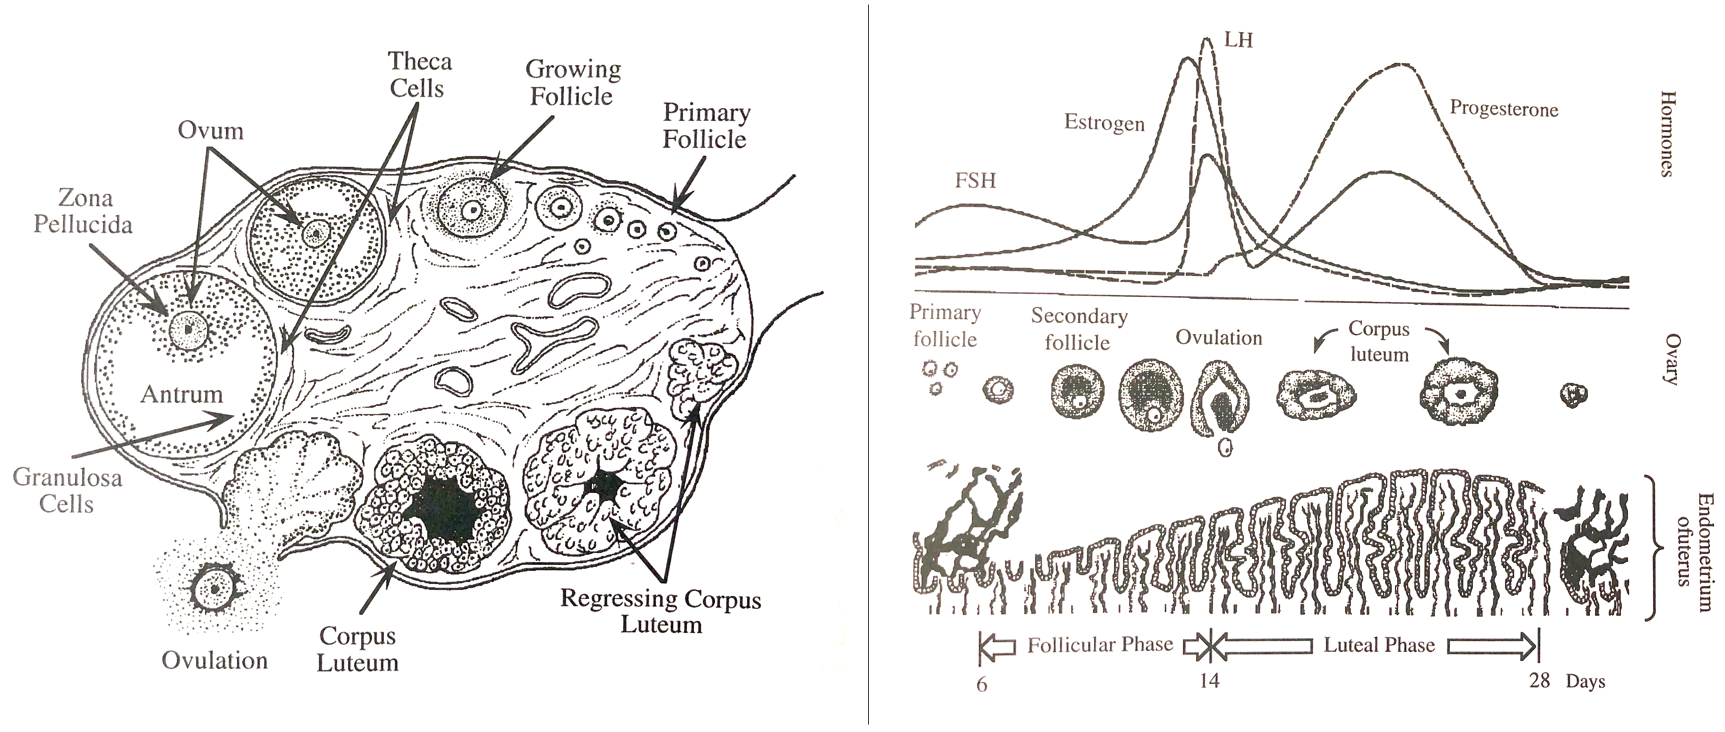
\includegraphics[width=\textwidth]{ovarian_cycle.png} \label{ovarian_cycle}
\caption{The ovarian cycle and its associated hormones.}
\end{figure}
\indent As we've mentioned previously, the \textbf{theca cells} convert cholesterol into \textbf{testosterone}, which diffuses into the follicle cells where it is converted into \textbf{estrogen}. Estrogen helps in the development of the primary follicle (i.e. the primary oocyte). Meanwhile, recall that the anterior pituitary secretes LH and FSH\textemdash LH affects the theca cells while FSH affects the follicle cells. As estrogen is being synthesized, the primary oocyte is developing so we have a proliferation of follicle cells. If we have more follicle cells, then we can synthesize more estrogen. This is where the first estrogen surge (the one in the follicular phase) comes from. It turns out that at low concentrations of estrogen there is a negative feedback on FSH production. However, as the follicle cells are growing, they reach a certain threshold level of estrogen where at these high concentrations, estrogen actually has a \textit{positive feedback} on the anterior pituitary and LH production. Thus, with a high level of estrogen production, we can now have the \textbf{LH surge}. \\
\indent Immediately following the LH surge, the levels of LH drop down to very low levels. This is because at ovulation the follicle cells become transformed into the \textbf{corpus luteum}, meaning they are no longer follicle cells and hence transiently lose their ability to produce estrogen. Since we no longer have the high concentration of estrogen, we lose the positive feedback on the anterior pituitary.\\
\indent Eventually, the corpus luteum becomes an endocrine gland and begins to synthesize estrogen and progesterone. Together, these hormones have a negative feedback on LH and FSH production in the anterior pituitary, and also on the hypothalamus on GnRH synthesis. Essentially, this prevents the primary follicle from developing, which is good because at this point there's no reason to have another primary follicle made. Remember, estrogen (in high concentrations) has a positive feedback, while estrogen and progesterone in the combination have a negative feedback. \\
\indent During pregnancy, things are a bit different. The acrosome of the spermatozoan allows for the digestion of the membrane of the secondary oocyte. After the nucleus of the sperm enteres the secondary oocyte, the \textbf{zona pellucida} changes and prevents any other spermatozoa from entering\textemdash this process is referred to as \textbf{fertilization}. At this point the secondary oocyte undergoes the second meiotic division to form the \textbf{ovum} and the polar body. The nucleus of the sperm and egg fuse to form the \textbf{zygote}, which now has 46 chromosomes. The zygote rapidly develops and in about 7 days attaches itself as a \textbf{blastocyst} to the \textbf{uterine lining}. When the implantation takes place the \textbf{placenta}, made up of maternal and fetal cell types, begins to form.\\
\indent For obvious reasons, we don't want the development of another primary follicle during pregnancy. Thus, throughout pregnancy, there are high levels of estrogen and progesterone. These high levels are maintained during the last six months of pregnancy, but for different reasons as we will discover. 
\begin{enumerate}
	\item During the first three months, the corpus luteum is still a viable gland and secretes estrogen and progesterone. The placenta is also an endocrine gland and synthesizes \textbf{chorionic gonadotropin (CG)}, which stimulates the corpus luteum to make estrogen and progesterone. CG is only made during the first three months of pregnancy. During this time, estrogen and progesterone work together to prevent the formation of primary follicles (and hence ovulation and menstruation as well) during pregnancy. The \textbf{mammary gland} is also sensitive to certain hormones during this time, such as \textbf{prolactin} that comes from the anterior pituitary and acts in a positive feedback manner on the mammary gland, and also \textbf{chorionic somatomammotropin (CS)} which comes from the placenta. CS and prolactin basically help the mammary gland grow. Estrogen and progesterone has positive feedback on the mammary glands as well. 
	\item During the last six months of pregnancy, CG is no longer made, so there is a loss of feedback to the corpus luteum. After three months, the corpus luteum breaks down and the supply of estrogen and progesterone from it comes to a halt. However, at this point in time the placenta itself starts to synthesize estrogen and progesterone.
\end{enumerate}

\subsection{Development}
The \textbf{coelom} is the body cavity, basically the thoracic cavity and abdominal cavity. After fertilization, we have \textbf{cleavage} of the zygote, where the zygote rapidly diveds into many smaller cells without an overall increase in size. \textbf{Gastrulation} then follows, where the cells of the zygote move to form the three primary germ layers (ectoderm, mesoderm, and endoderm) of the organism. The next developmental stage is \textbf{neurulation}, where we begin to see the formation of the nervous system, the first organ system to begin differentiation. \textbf{Neural crest} formation is the fifth developmental stage, which helps to form parts of the nervous system, skull, and sensory organs. The last stage of development is \textbf{organogenesis}.
\begin{equation}
\begin{split}
\text{Fertilization}\rightarrow\text{Cleavage}\rightarrow\text{Gastrulation}\rightarrow\text{Neurulation}\rightarrow\text{Neural Crest Formation}\rightarrow\text{Organogenesis}
\end{split}
\end{equation}
\noindent Let's take a look at development in the frog to see an example of vertebrate development. In the unfertilized egg there is a large amount of yolk that resides in the \textbf{vegetal pole} (i.e. the lower hemisphere), which will act as food for the developing embryo. The \textbf{animal pole} (i.e. the upper hermisphere) contains mainly cytoplasm. The \textbf{gray crescent} is located on the \textbf{dorsal aspect} (i.e. the future back) of the egg, opposite to where the sperm penetrates the egg's membrane. It eventually is where we will find the spinal cord and brain. \\
\indent Once the zygote has formed, it undergoes special cell division to increase its mass but not its overall size. The individual cells involved in this growth are called \textbf{blastomeres}. Eventually, a small, solid ball of cells will be formed called a \textbf{morula}. Further cellular division results in the formation of a hollow ball of cells called the \textbf{blastula}, which includes a fluid-filled cavity called the \textbf{blastocoel}. These different initial stages are shown in \textbf{Fig. \ref{embryonic_development}}.\\
\begin{figure}[!ht]
\centering
\includegraphics[width=\textwidth]{embryonic_development.png} \label{embryonic_development}
\caption{Different stages in embryonic development.}
\end{figure}
\indent During \textbf{gastrulation}, rearrangement of cells occurs. Not far from the gray crescent, an opening develops in the blastula called the \textbf{blastopore}. Cells from the animal pole begin to migrate inwards through the \textbf{dorsal lip} of the blastopore. As this outer layer of cells migrates inward, they form a second layer of cells immediately below. The blastocoel is reduced in size and is ultimately eliminated\textemdash in its place, a new cavity is formed called the \textbf{archenteron}. At this stage, the embryo is referred to as a \textbf{gastrula}. Invagination of the outer cell layer produce two cell layers: the \textbf{ectoderm} (outer layer) and \textbf{endoderm} (inner layer). A layer of \textbf{mesoderm} will later form between these two cell layers. The different stages of gastrulation are shown in \textbf{Fig. \ref{gastrulation}}. In general, it seems that the generation of three cell layers has been conserved through the evolutionary process.\\
\begin{figure}[!ht]
\centering
\includegraphics[width=0.75\textwidth]{gastrulation.png} \label{gastrulation}
\caption{The process of gastrulation.}
\end{figure}
\indent Here are important \textit{developmental fates} to remember:
\begin{enumerate}
	\item \textbf{Endoderm:} inner lining of the digestive and respiratory tracts, and major glands of the body like the liver and pancreas.
	\item \textbf{Mesoderm:} notochord, heart, skeleton, muscle, outer coverings of internal organs, and reproductive organs.
	\item \textbf{Ectoderm:} skin, lens of the eye, brain and nervous system.
\end{enumerate}
\noindent These are just a few of the developmental fates of these cell layers. Now, during the next stage of development, \textbf{neurulation}, the ectoderm, mesoderm, and endoderm begin to form the structures that will eventually define the embryo and later the adult. Notably, the formation of the \textbf{notochord} takes place along the body midline, and is derived from the \textit{mesoderm}. Superior to the notochord is a mass of \textit{ectodermal cells} called the \textbf{neural plate}, which begins to fold in on itself and form the \textbf{neural groove}. As the neural groove forms, the mesoderm is also split and forms the coelom (i.e. the body cavity). The neural groove goes on to form the \textbf{neural tube}, which will eventually encase the spinal cord (encased in the \textit{spinal column}), and anterior to the spinal cord will form the brain. In other words, the neural plate, which is composed of ectodermal cells, gives rise to the nervous system. This tissue is referred to as \textbf{primordium}, and the embryo is referred to as a \textbf{neurula} during this stage of development. \textbf{Fig. \ref{neurulation}} shows the formation of the neural tube during neurulation.\\
\begin{figure}[!ht]
\centering
\includegraphics[width=0.75\textwidth]{neurulation.png} \label{neurulation}
\caption{Neural tube formation.}
\end{figure}\indent When the edges of the neural groove fused together and become the neural tube, specialized ectodermal cells were left outside the tube and are called \textbf{neural crest cells}. These cells begin to form various parts of the body, such as the sensory cells of the head, the adrenal medulla, and other things. This process is called \textbf{neural crest formation}.\\
\indent \textbf{Organogenesis} first begins with interactions between the ectoderm and mesoderm. The neural tube becomes longer and thinner. Mesodermal cells migrate towards the neural tube and eventually form the vertebral column. The brain and optic vesicles begin to form. As the neural tube continues to form, segments of mesodermal tissue called \textbf{somites} begin to appear, which eventually gives rise to the vertebrae, connective tissue, and muscles of the body.\\

\subsection{Developmental Mechanisms}
There are two general classes of interaction associated with the differentiation of cells that we need to consider: intracellular and intercellular interactions. Intracellular interactions usually result in the setting up of a \textit{prepattern}, while the intercellular interactions usually undergo \textit{developmental induction}. \\
\indent Recall that after fertilization and induction of development, the gray crescent forms at a point opposite to where the sperm penetrated the egg. The formation of the gray crescent is due to an intracellular interaction, and is not a prepatterned phenomenon simply because of the fact that the entry of the sperm in the animal half of the cell is random. However, once entry is made and the gray crescent forms, the dorsal midline is established. This allows us to define directions. In other words, prior to the first cellular division, the axes of the organism are already established. Hans Spemann showed that the gray crescent is essential for complete embryonic development in the 1920s.

\subsection{Human Embryo Development}
Recall that the \textbf{blastocyst} is a hollow ball of cells with a mass of cells on one side. The surrounding cells that form the ball are called the \textbf{trophoblast}, and the other are called the \textbf{inner cell mass}. If the lining of the uterus is prepared to receive the embryo, then it will implant. Otherwise, the embryo is rejected and sloughed off during the next menstrual period. After implantation, the trophoblastic cells grow into the lining of the uterus. (In fact, the cells of the trophoblast grow little finger-like projections into the uterus.)\\
\indent For nourishment, blood vessels from the umbilical cord grow into the projections of the trophoblast. There is a layer of cells between the trophoblast and the fetal blood vessels called the \textbf{chorion}, which preserves the barrier between the mother's and fetus's blood (but diffusion of nutrients and waste products may still occur). This whole exchange apparatus is called the \textbf{placenta}.\\
\indent The \textbf{inner mast cells} will undergo changes similar to those in the frog to form the three basic germ layers. We also have the \textbf{primitive streak}, which is equivalent to the neural plate in frogs, that forms in the ectoderm. Cells from the primitive streak migrate down between the ectoderm and endoderm to become the mesoderm. Further folding of the primitive streak gives rise to a neural groove and then a neural tube, etc. So, the formation of the primitive streak in mammals marks the beginning of gastrulation, which is quickly followed by neurulation. Cell fate determination from the three germ layers in humans is basically the same as in frogs.\\
\indent The embryo cannot implant if the uterus is not receptive\textemdash that is, if it is not \textbf{quiescent}. Furthermore, pregnancy will not be maintained by the uterus even after implantation unless it remains quiescent. So, to maintain the uterine lining through the first part of pregnancy, the trophoblastic cells secrete \textbf{chorionic gonadotropin (CG)}, which is a hormone that causes the corpus luteum to continue to produce estrogen and progesterone. Eventually, the placenta can take over the production of estrogen and progesterone itself and the corpus luteum is no longer needed.\\
\indent The placenta secretes increasing amounts of estrogen and progesterone, but the levels of estrogen increase faster than those of progesterone. At some point near the end of pregnancy, the levels of progesterone plateau, and at a critical ratio of [estrogen]:[progesterone], the uterus is no longer quiescent; it begins to have contractions. The smooth muscle of the uterus contracts, putting the walls of the uterus under tension that thus sends nerve impulses to the hypothalamus. The hypothalamus then sends signals to the posterior pituitary to release \textbf{oxytocin}, which is a strong inducer of more contractions of the smooth muscle of the uterus. Oxytocin also stimulates the production and secretion of prostaglandins that further induce contractions. All of these hormones and nerves form a \textit{positive feedback system}. We call the birth process \textbf{parturition}. \\
\indent Milk production and milk ejection are two important processes in lactation. There are epithelial cells within the breast that make up the glands that produce the milk, and around these cells, we have the myoepithelial cells that can contract around the milk glands, ejecting the milk. Production of milk is stimulated by the suckling of the infant on the mother's nipple. The nipple sends a nervous impulse to the hypothalamus, which responds by releasing \textbf{PRH (prolactin releasing hormone)}, which acts on the anterior pituitary. PRH stimulates the anterior pituitary to release \textbf{prolactin}, which goes into the bloodstream and stimulates the epithelial cells in the breasts which comprise the milk glands to produce more milk. Suckling on the nipple also tells the hypothalamus to send a nervous signal to the posterior pituitary and release \textbf{oxytocin}, which causes contraction of the myoepithelial cells in the breast to squeeze the milk out.

\subsection{Endocrinology}
Hormones can generally be divided into \textit{peptide} hormones (e.g. insulin), \textit{amine} hormones (e.g. epinephrine or adrenaline, which are classified as \textbf{catecholamines}), and \textit{steroids} (e.g. progesterone and estrogen). \textit{Catecholamines} are monoamine neurotransmitters, which are organic compounds that have a catechol (benzene with two hydroxyl side groups next to each other) and a side-chain amine. Hormones are released by endocrine organs into the blood and travel by way of the circulatory system to various target tissues. To illustrate the importance of hormones, let's consider the action of the catecholamine epinephrine (adrenaline) on a typical hepatic (liver) cell. When the body is under some type of stress like physical exercise or even fright, an increased need for glucose arises.\\
\indent One a stress has been perceived, the nervous system responds by signaling the adrenal medulla (part of the adrenal gland that sits on top of the kidneys) to release epinephrine into the extracellular fluid. Epinephrine diffuses into the blood, and the \textbf{$\beta$-adrenergic receptors} on hepatic cells bind to epinephrine and cause the activation of \textbf{adenylate cyclase} (bound on the cytoplasmic membrane surface), which increases the concentration of cAMP (cyclic adenosine monophosphate, a second messenger) in the cell. $\beta$-adrenergic receptors are a type of \textit{G-protein coupled receptors}. GTP-bound state corresponds to the active state, while GDP-bound state corresponds to the inactive state. The increase in cAMP concentration allows cAMP to interact with \textit{protein kinase A} (PKA) and help it phosphorylate an enzyme called \textbf{\textit{glycogen phosphorylase}}. Once glycogen phosphorylase has become phosphorylated, it is now an active enzyme and catalyzes the conversion of glycogen into glucose.\\
\indent \textbf{Cholera} is an intestinal disorder caused by the \textit{Vibrio cholerae} bacterium. The major symptom of this disorder is \textbf{diarrhea}, and if left untreated will result in severe dehydration and eventual death. This toxin binds to the active state of the G protein and prevents GTP from being hydrolyzed to GDP. This means that the adenylate cyclase enzyme is continually active and massive amounts of cAMP are synthesized. cAMP causes the intestinal cells to secrete digestive fluids. \\
\indent Let's consider another example, this time involving the water-soluble peptide hormone \textbf{gastrin} that stimulates the secretion of HCl and pepsinogen from the stomach in response to stimulation from the vagus nerve and partially digested protein. Gastrin first binds to a GPCR, activating an associated G-protein that can now interact with the membrane enzyme \textbf{phospholipase C (PLC)}, and this interaction induces PLC to hydrolyze phosphatidyl-inositol-4,5-biphosphate (PIP\textsubscript{2}) to inositol-1,4,5-triphosphate (IP\textsubscript{3}) and 1,2-diacylglycerol (DAG). IP\textsubscript{3} is a second messenger that interacts with the IP\textsubscript{3}-sensitive calcium ion channels in the endoplasmic reticulum membrane, stimulating the release of \ce{Ca^{2+}} ions into the cytosol from the ER lumen. Meanwhile, DAG, diffusing through the plasma membrane, interacts with \textbf{protein kinase C} and stimulates that kinase with the help of \ce{Ca^{2+}} to phosphorylate an unknown protein which in turn causes HCl secretion into the lumen of the stomach. \\
\indent Another example of a peptide hormone in action involves insulin, which is a water-soluble peptide hormone that binds to a specific trans-membrane receptor in the cell membranes of liver, fat, and muscle cells. Once insulin binds to the receptor on the cell surface, the cytoplasmic portion of the receptor is converted into a tyrosine kinase that autophosphorylates the amino acid tyrosine found within the cytoplasmic portion of the receptor. This acts to further enhance the activity of the tyrosine kinase. Presumably, the insulin receptor can also internalize and somehow act as a second messenger. This action, along with enhanced tyrosine kinase activity, leads to the internalization of glucose into the cells. The actual events in the insulin signaling mechanism that leads to the uptake of glucose are somewhat obscure at the present time.\\
\indent While these show a lot about the some of the many different pathways in cell signaling, kind of the main thing to pay attention to is that peptide and catecholamine hormones always involve some signaling intermediates because they can't diffuse freely through the membrane. Contrast this with steroid and thyroid hormones, which are lipid soluble hormones that can pass through the cell's plasma membrane and interact with a receptor either in the cytosol or in the nucleus. \textbf{Thyroid hormones} can diffuse across the plasma membrane and into the nucleus where they ind with specific receptors. The hormone receptor complex then activates transcription essential for certain metabolic processes; indeed, thyroid hormones help to regulate growth and differentiation and they can stimulate the breakdown of proteins, fats, and glucose.\\
\indent There are four major types of regulatory mechanisms in endocrinology: endocrine, neuroendocrine, paracrine, and autocrine. We go over an example of each here: 
\begin{itemize}
	\item \textbf{Endocrine Regulation:} The \textbf{pancreas} secretes insulin and glucagon, which are two hormones that are important in maintaining the proper levels of blood glucose. Both of these hormones are secreted from clusters of specialized cells called the \textbf{islets of Langerhans}. Insulin is secreted by the $\beta$ cells, while glucagon is secreted by the $\alpha$ cells. An increase in blood glucose stimulates the $\beta$ cells to produce insulin and excrete it into the blood, which goes to the liver, fat, and muscle cells and tells them to uptake glucose, thus decreasing blood glucose levels. Similarly, a decrease in blood glucose stimulates the $\alpha$ cells to produce glucagon and excrete it into the blood, which goes to the lever and fat cells and tells them to release glucose and fatty acids, thus increasing blood glucose levels. This is an example of \textbf{negative feedback}.
	\item \textbf{Neuroendocrine Regulation:} In this case, the hormone is not released for an endocrine cell, but rather from a nerve cell which releases its neurotransmitter in the form of a hormone into the blood. For example, the \textbf{adrenal medulla} can receive sensory input from a sympathetic nerve, which tells it to release epinephrine into the blood. Other examples of neuroendocrine regulation involve the \textbf{hypothalamus} and the \textbf{pituitary gland}. The pituitary gland can be divided into the \textbf{anterior} and \textbf{posterior pituitary}.
	\item \textbf{Paracrine Regulation:} In paracrine regulation, the chemical that acts as a signal is released from one cell and influences a cell immediately adjacent to it. An example of such a paracrine cell would be \textbf{mast cells}, which contain large amounts of \textbf{histamine}. The substances released by the paracrine cell are generally dumped into the extracellular space and not into the bloodstream. Other examples of a paracrine signal would be neurohormones and neurotransmitters.
	\item \textbf{Autocrine Regulation:} In autocrine regulation, cells can release certain chemicals which they can then respond to themselves. For example, certain cells can release growth factors which can then bind to specific receptors on the membrane of that same cell. Thus, the cells that released the growth hormone are stimulated to grow.
\end{itemize}

\subsection{The Pituitary Gland}
The posterior pituitary releases \textbf{oxytocin} and \textbf{antidiuretic hormone}, which are synthesized in specific cells of the hypothalamus. Oxytocin stimulates female uterine contraction in a positive feedback loop while antidiuretic hormone (ADH) stimulates water and \ce{Na^{2+}} reabsorption int he kidneys and also helps to increase the blood volume/pressure. The ADH that is synthesized in the nerve cell bodies in the hypothalamus are packaged into vesicles and transported down the axon to the terminal bouton in the posterior pituitary. A nerve impulse propagates down that same axon and causes the release of these hormones into a system of nearby capillaries. ADH helps prevent \textbf{diuresis}, which is the excessive loss of urine.\\
\indent The anterior pituitary secretes six major hormones: thyroid stimulating hormone (TSH), adrenocorticotropic hormone (ACTH), follicle stimulating hormone (FSH), luteinizing hormone (LH), growth hormone (GH), and prolactin (PRL). These hormones are regulated by a second set of hormones stored in the ypothalamic nerves. For example, the hypothalamus has nerve cells that contain thyrotropin releasing hormone (TRH). When this nerve is stimulated, it secretes TRH into a set of capillaries which extend into the anterior pituitary. TRH stimulates the synthesis and release of TSH, which in turn binds to specialized receptors in the thyroid gland and causes the release of thyroxine. Thyroxine increases the rate of metabolism and growth as a part of a negative feedback loop.

\subsection{Immunology}
Blood contains \textbf{erythrocytes} (red blood cells), \textbf{leukocytes} (white blood cells), and platelets. Erythrocytes are produced in the marrow of the sternum, ribs, and vertebrae, while leukocytes are produced partially in the tissues of the lymph and partly in the bone marrow.\\
\indent There are six types of leukocytes found in the blood, but we are only interested in three of them: \textbf{monocytes}, \textbf{neutrophils}, and \textbf{lymphocytes}. Monocytes and neutrophils are considered to be \textbf{phagocytes}, which, along with \textbf{mast cells} and a variety of other cell types, participate in the \textit{immune response}. 
\begin{itemize}
	\item \textbf{Mast cells} are derived from leukocytes and then migrate out into the tissues where they reside. When mast cells are stimulated, they release \textbf{histamine} which acts on endothelial cells and causes an increased permeability to cells like neutrophils, allowing neutrophils easy access to the surrounding tissue in order to defend against foreign pathogens.
	\item \textbf{Phagocytes} include monocytes (i.e. \textbf{macrophages} when they leave the blood and enter into the tissues) and neutrophils. These cells are the primary cell types that attack and destroy foreign bacteria and viruses. They do this by the process of \textbf{phagocytosis}, engulfing the foreign invader by \textbf{endocytosis}. 
	\item \text{Lymphocytes} are derived from either the \textbf{thymus} gland (which produces \textbf{T lymphocytes}) or elsewhere from places that produce \textbf{B lymphocytes}. T cells are responsible for \textit{cell-mediated immunity}. These cells are responsible for the destruction of foreign microorganisms and other harmful agents. There are three types of T cells: cytotoxic/killer T cells, helper T cells, and suppressor T cells. B cells are responsible for \textit{humoral mediated immunity}. Upon infection, B cells can differentiate into \textbf{plasma cells} that can synthesize and secrete antibodies. \textbf{Antibodies} are proteins that are synthesized in response to an \textbf{antigen}, which is simply a foreign substance with high MW.
\end{itemize}
\noindent Let's go over the two types of general immune responses\textemdash cell-mediated immunity and humoral mediated immunity\textemdash in more detail:
\begin{itemize}
	\item \textbf{Cell-Mediated Immunity:} Macrophages engulfs a foreign particle and phagocytizes it. The antigenic fragments released into the cytosol of the macrophage are transported to the macrophage's membrane, where they bind to the \textbf{major histocompatibility complex protein, class 1 (MHCI)}. Certain receptors on \textbf{cytotoxic T cells} recognize the antigen-MHCI complex on the macrophage and bind to it, stimulating the release of growth factor \textbf{interleukin-1 (IL-1)} from the macrophage. The cytotoxic T cell also releases \textbf{interleukin-2 (IL-2)}. IL-1, IL-2, and other interleukins released by \textbf{helper T cells} (discussed below) stimulate the synthesis of more cytotoxic T cells. These killer T cells proliferate and bind to the invading foreign cells bearing the antigen, causing them to lyse.
	\item \textbf{Humoral Mediated Immunity:} B cells have \textbf{MHC class 2 (MHCII) proteins} and antibodies on their surface. When a B cell finds an antigen that has specifically bound to its antibody, it engulfs that antigen-antibody complex and transports a portion of that antigen to the MHCII protein, effectively `displaying' the complex on the surface of its membrane. \textbf{Helper T cells} with the right receptors are able to bind to the antigen-MHCII complexes, stimulating the helper T cells to release interleukins (a \textbf{lymphokine}). This stimulates the B cells to proliferate and form \textbf{plasma cells}, which in turn produce a vast amount of \textbf{antibodies} specific to the original antigen. When these circulating antibodies bind to the antigen, they act as a tag that signals circulating phagocytes to engulf the antigen-antibody complex and destroy it. The human immunodeficiency virus (HIV) acts at the level of the helper T cells by infecting them.
\end{itemize}

\subsection{Antibodies}
Most immunoglobulins (antibodies) are composed of 4 subunits arranged in a `Y' configuration. There are 2 light chains and 2 heavy chains. These subunits are joined to one another by disulfide bonds. Within each heavy and light chain are \textbf{variable domains} and \textbf{constant domains}. \\
\indent At the terminal ends of the heavy and light chains are variable (V) regions that can differ in amino acid sequence from immunoglobulin to immunoglobulin. The constant (C) regions of the heavy and light chains are found in the lower portions of the immunoglobulin. The \textbf{antigen binding site} for a particular antibody is located at the end of the variable regions of the heavy and light chains.\\
\indent Two other regions of the immunoglobulin are important: the diversity (D) and the joining (J) region. We show a picture of the general antibody structure in \textbf{Figure \ref{antibody_structure}}.
\begin{figure}[h!]
\centering
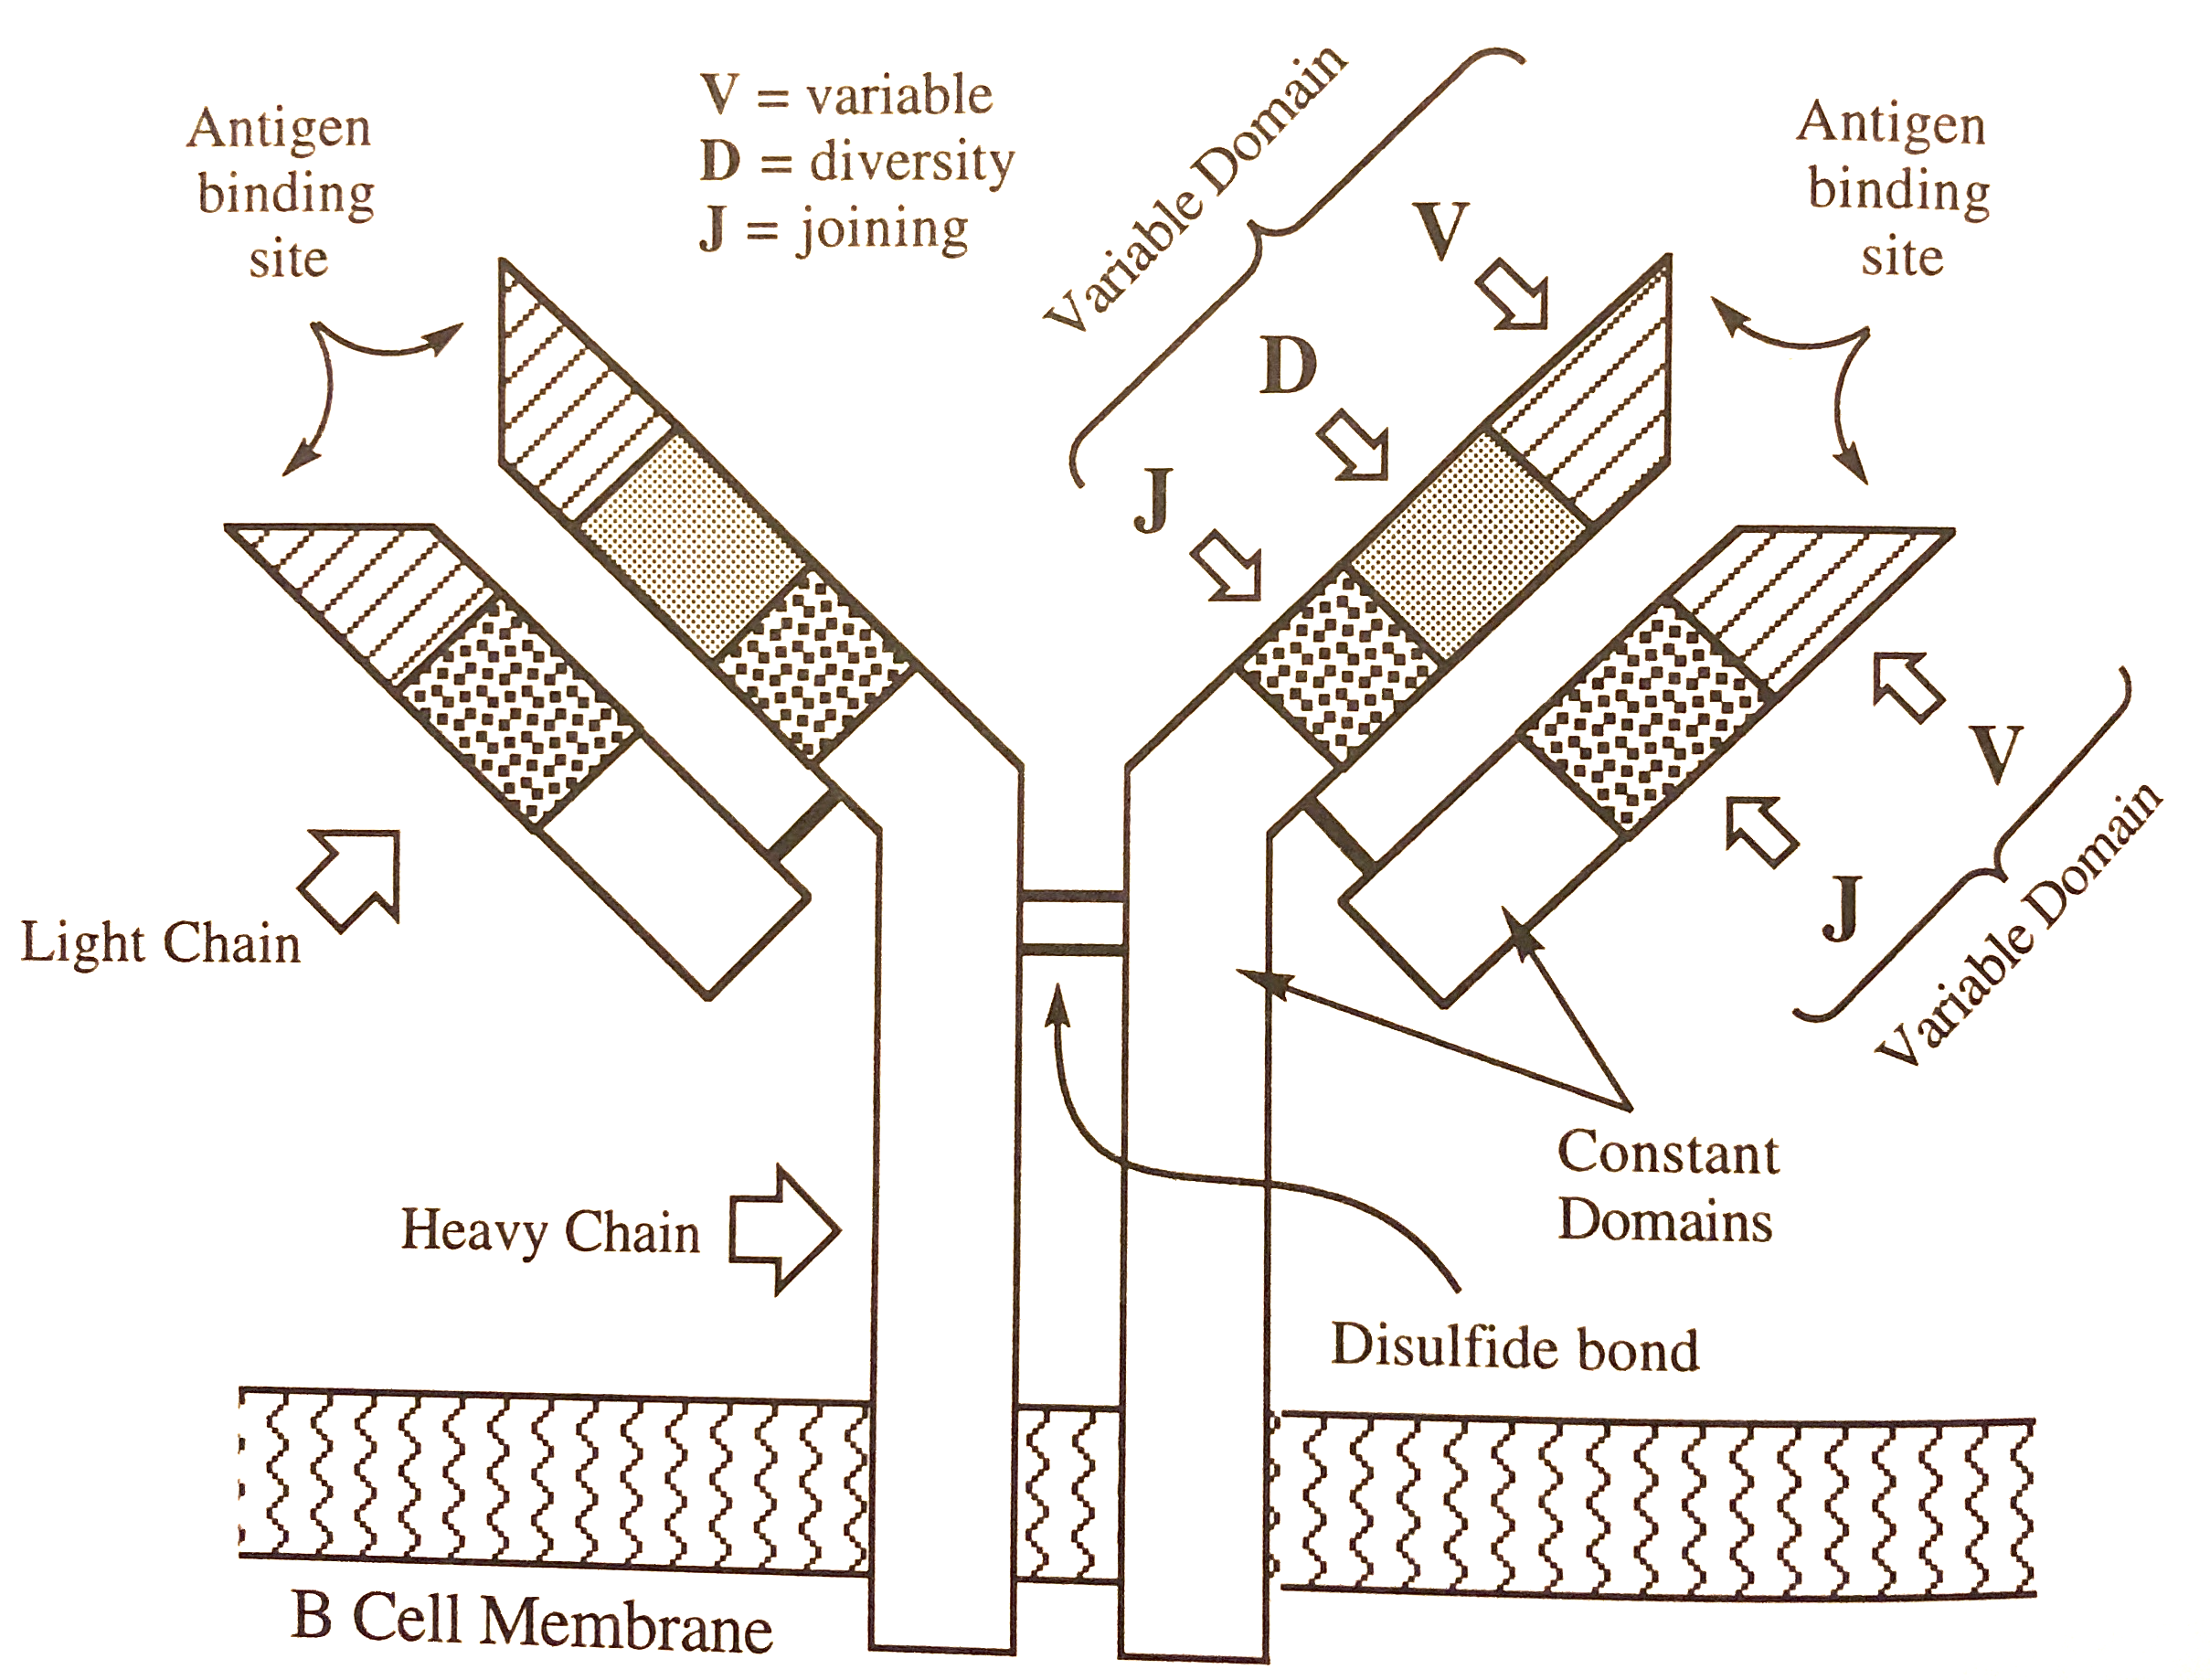
\includegraphics[width=0.7\textwidth]{antibody_structure.png} \label{antibody_structure}
\caption{Generalized antibody structure.}
\end{figure}
\noindent There are five classes of immunoglobulins that differ in the composition of their heavy chains:
\begin{itemize}
	\item \textbf{IgA:} Found in milk and helps to protect nursing infants.
	\item \textbf{IgD:} Has unknown function.
	\item \textbf{IgE:} Binds to mast cells and is involved in the allergic reaction.
	\item \textbf{IgG:} The only antibody able to cross the placenta. It is also the most abundant and is produced within days after the IgM antibody is secreted.
	\item \textbf{IgM:} Produced a few days after detection of an antigen and it is the first antibody produced in response to an antigen.
\end{itemize}
\noindent Antibodies simply recognize and identify foreign antigens, and can have different mechanisms by which to accomplish this function:
\begin{itemize}
	\item \textbf{Direct Blocking:} The antibody directly blocks the foreign invader from gaining access to host cells. This is accomplished by the antibodies binding to the antigens or other parts of the pathogen.
	\item \textbf{Complement:} An antibody has already recognized and bound to a specific antigen on a bacterial cell that is considered an intruder, and a complement protein (plasma protein) this antigen-antibody complex and binds to the Fc domain of the antibody. After a series of reactions, the complement protein is activated and triggers an immune response. Further reactions form a \textbf{membrane attack complex (MAC)} that inserts into the bacterial cell's membrane and forms a channel that lets water into the cell, causing it to swell with water and eventually lyse.
	\item \textbf{Coating the Cell Surface:} Antibodies can bind to specific antigens on the surface of a bacterial cell and coat the cell surface. Once the antibodies have attached to the bacterial cell, phagocytes and/or killer T cells can bind to the terminal portion of the Fc domain of the antibodies and begin to engulf the foreign invader.
\end{itemize}

\subsection{T Cells}
The receptors for T cells are composed of two polypeptide chains, each with a constant and variable domain. Within a variable domain in each polypeptide we find a variable (V) region and a joining (J) region. On one of the polypeptide chains is a diversity (D) region. 
\begin{figure}[h!]
\centering
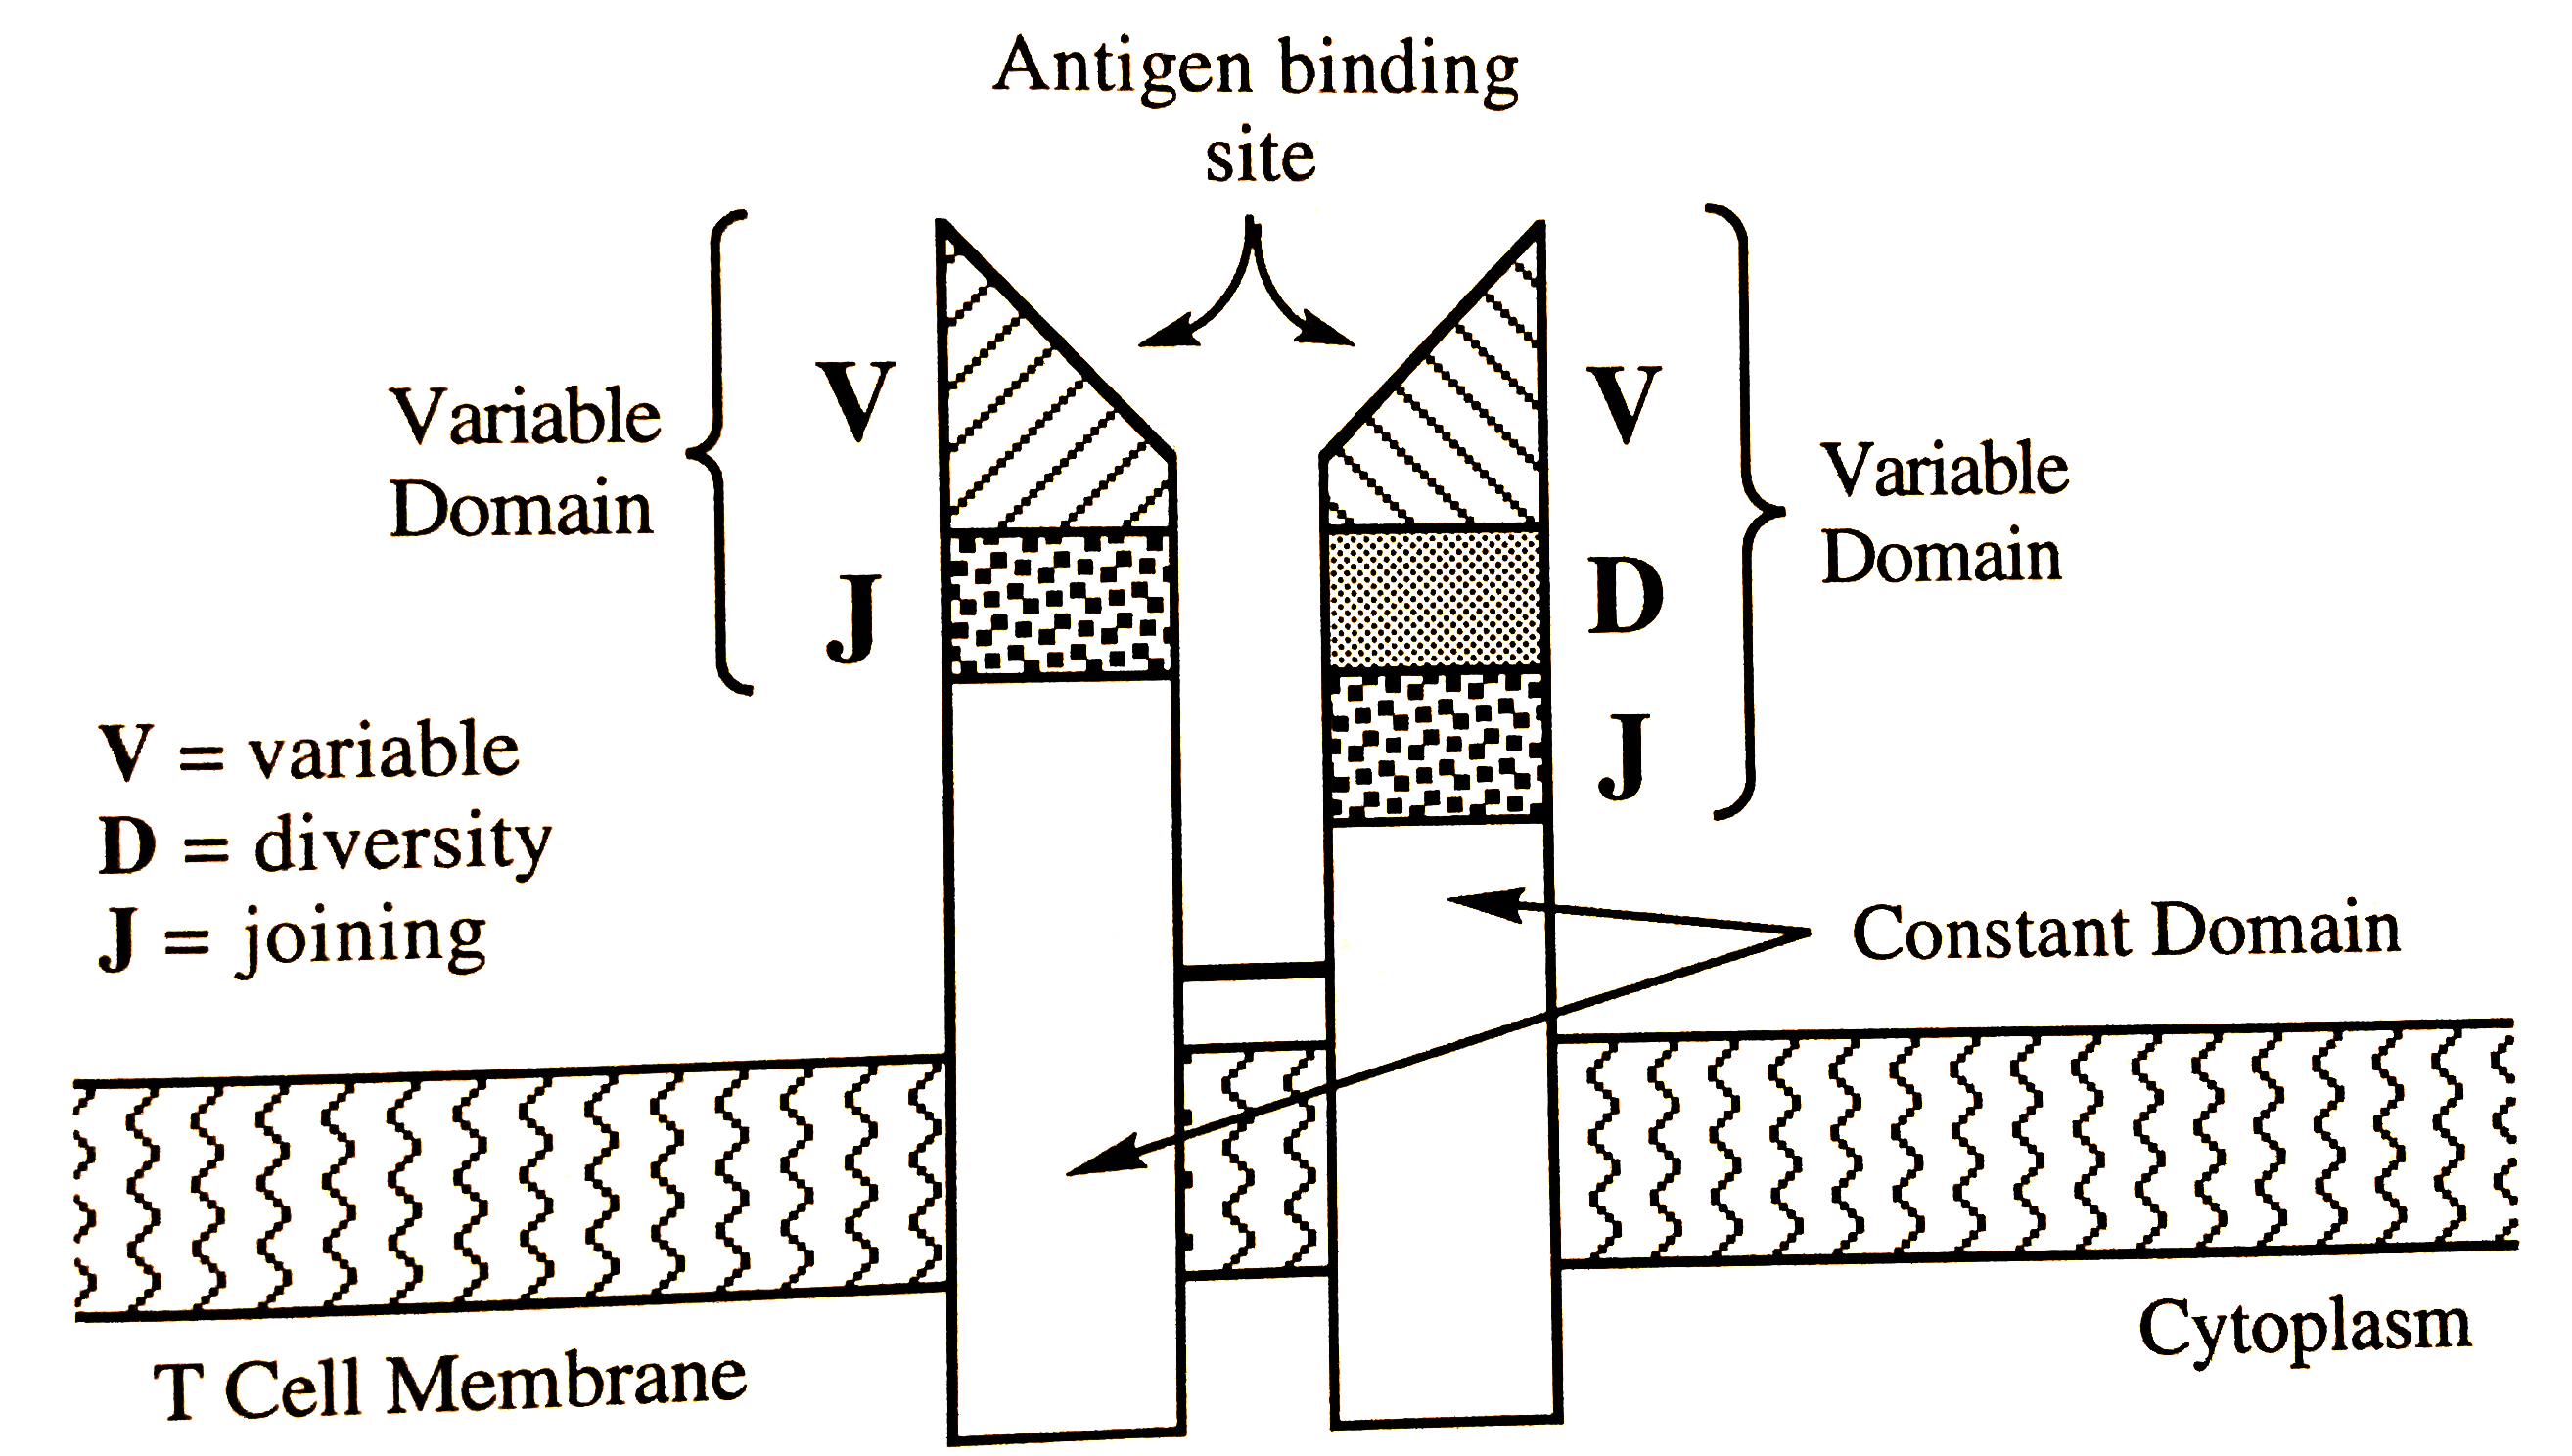
\includegraphics[width=0.55\textwidth]{t_cell_receptor.png} 
\caption{Example of T-cell Receptor Structure}
\end{figure}
\noindent If a virus infects a host cell, then that virus will begin to take over the host's metabolic machinery. As this happens some of the viral antigens are transported to the surface of the host cell where they can complex with a MHCI protein receptor, which are found on almost every one of our cells. The antigen-MHCI complex is recognized by the cytotoxic T cells, which induce lysis in the host cell. Immature helper T cells recognize macrophages which have presented an antigen on their MHCII receptors. Binding induces the macrophage to synthesize and release IL-1, which acts on the immature helper T cell and causes it to release IL-2, further stimulating the immature helper T cell to proliferate into a mature helper T cell. The mature form of the helper T cell secretes IL-2 which can activate cytotoxic T cells, B cells, and more helper T cells. 

\subsection{Immunology\textemdash Generalized Review}
Let's summarize the basic events in humoral and cellular immunity:
\begin{enumerate}
	\item A virus/bacterium enters the body by the blood and is engulfed by a macrophage.
	\item On the surface of the macrophage are MHCI receptors and MHCII receptors.
	\item A MHCII receptor presents the viral antigen to the receptor of a helper T cell, causing the macrophage to release IL-1 that stimulates the helper T cell to proliferate. 
	\item The helper T cell is stimulated to release IL-2 which enhances proliferation of helper T cells.
	\item A B cell with a MHCII protein presents viral antigen to helper T cells, and the IL-2 released from helper T cells stimulates B cells to proliferate.
	\item B cells produce plasma cells and memory B cells. Memory B cells `remember' antigen and proliferate faster during a future invasion of the same virus. Plasma cells secrete antibodies specific for the viral antigen. 
	\item The antibodies respond by direct block, complement, and cell surface coating.
	\item IL-2 from the helper T cells stimulates cytotoxic T cells which have bound to the MHCI protein-antigen complex of an infected cell to lyse the infected cell.
	\item Interferon is secreted by the infected host cell and acts on the cytotoxic T cell to help enhance the immune response.
	\item Cytotoxic T cell also make memory T cells, which will proliferate faster during a future invasion fo the same virus.
\end{enumerate}
\textbf{Fig. \ref{immune_pathway}} shows a diagram that basically summarizes the above information.
\begin{figure}[!ht]
\centering
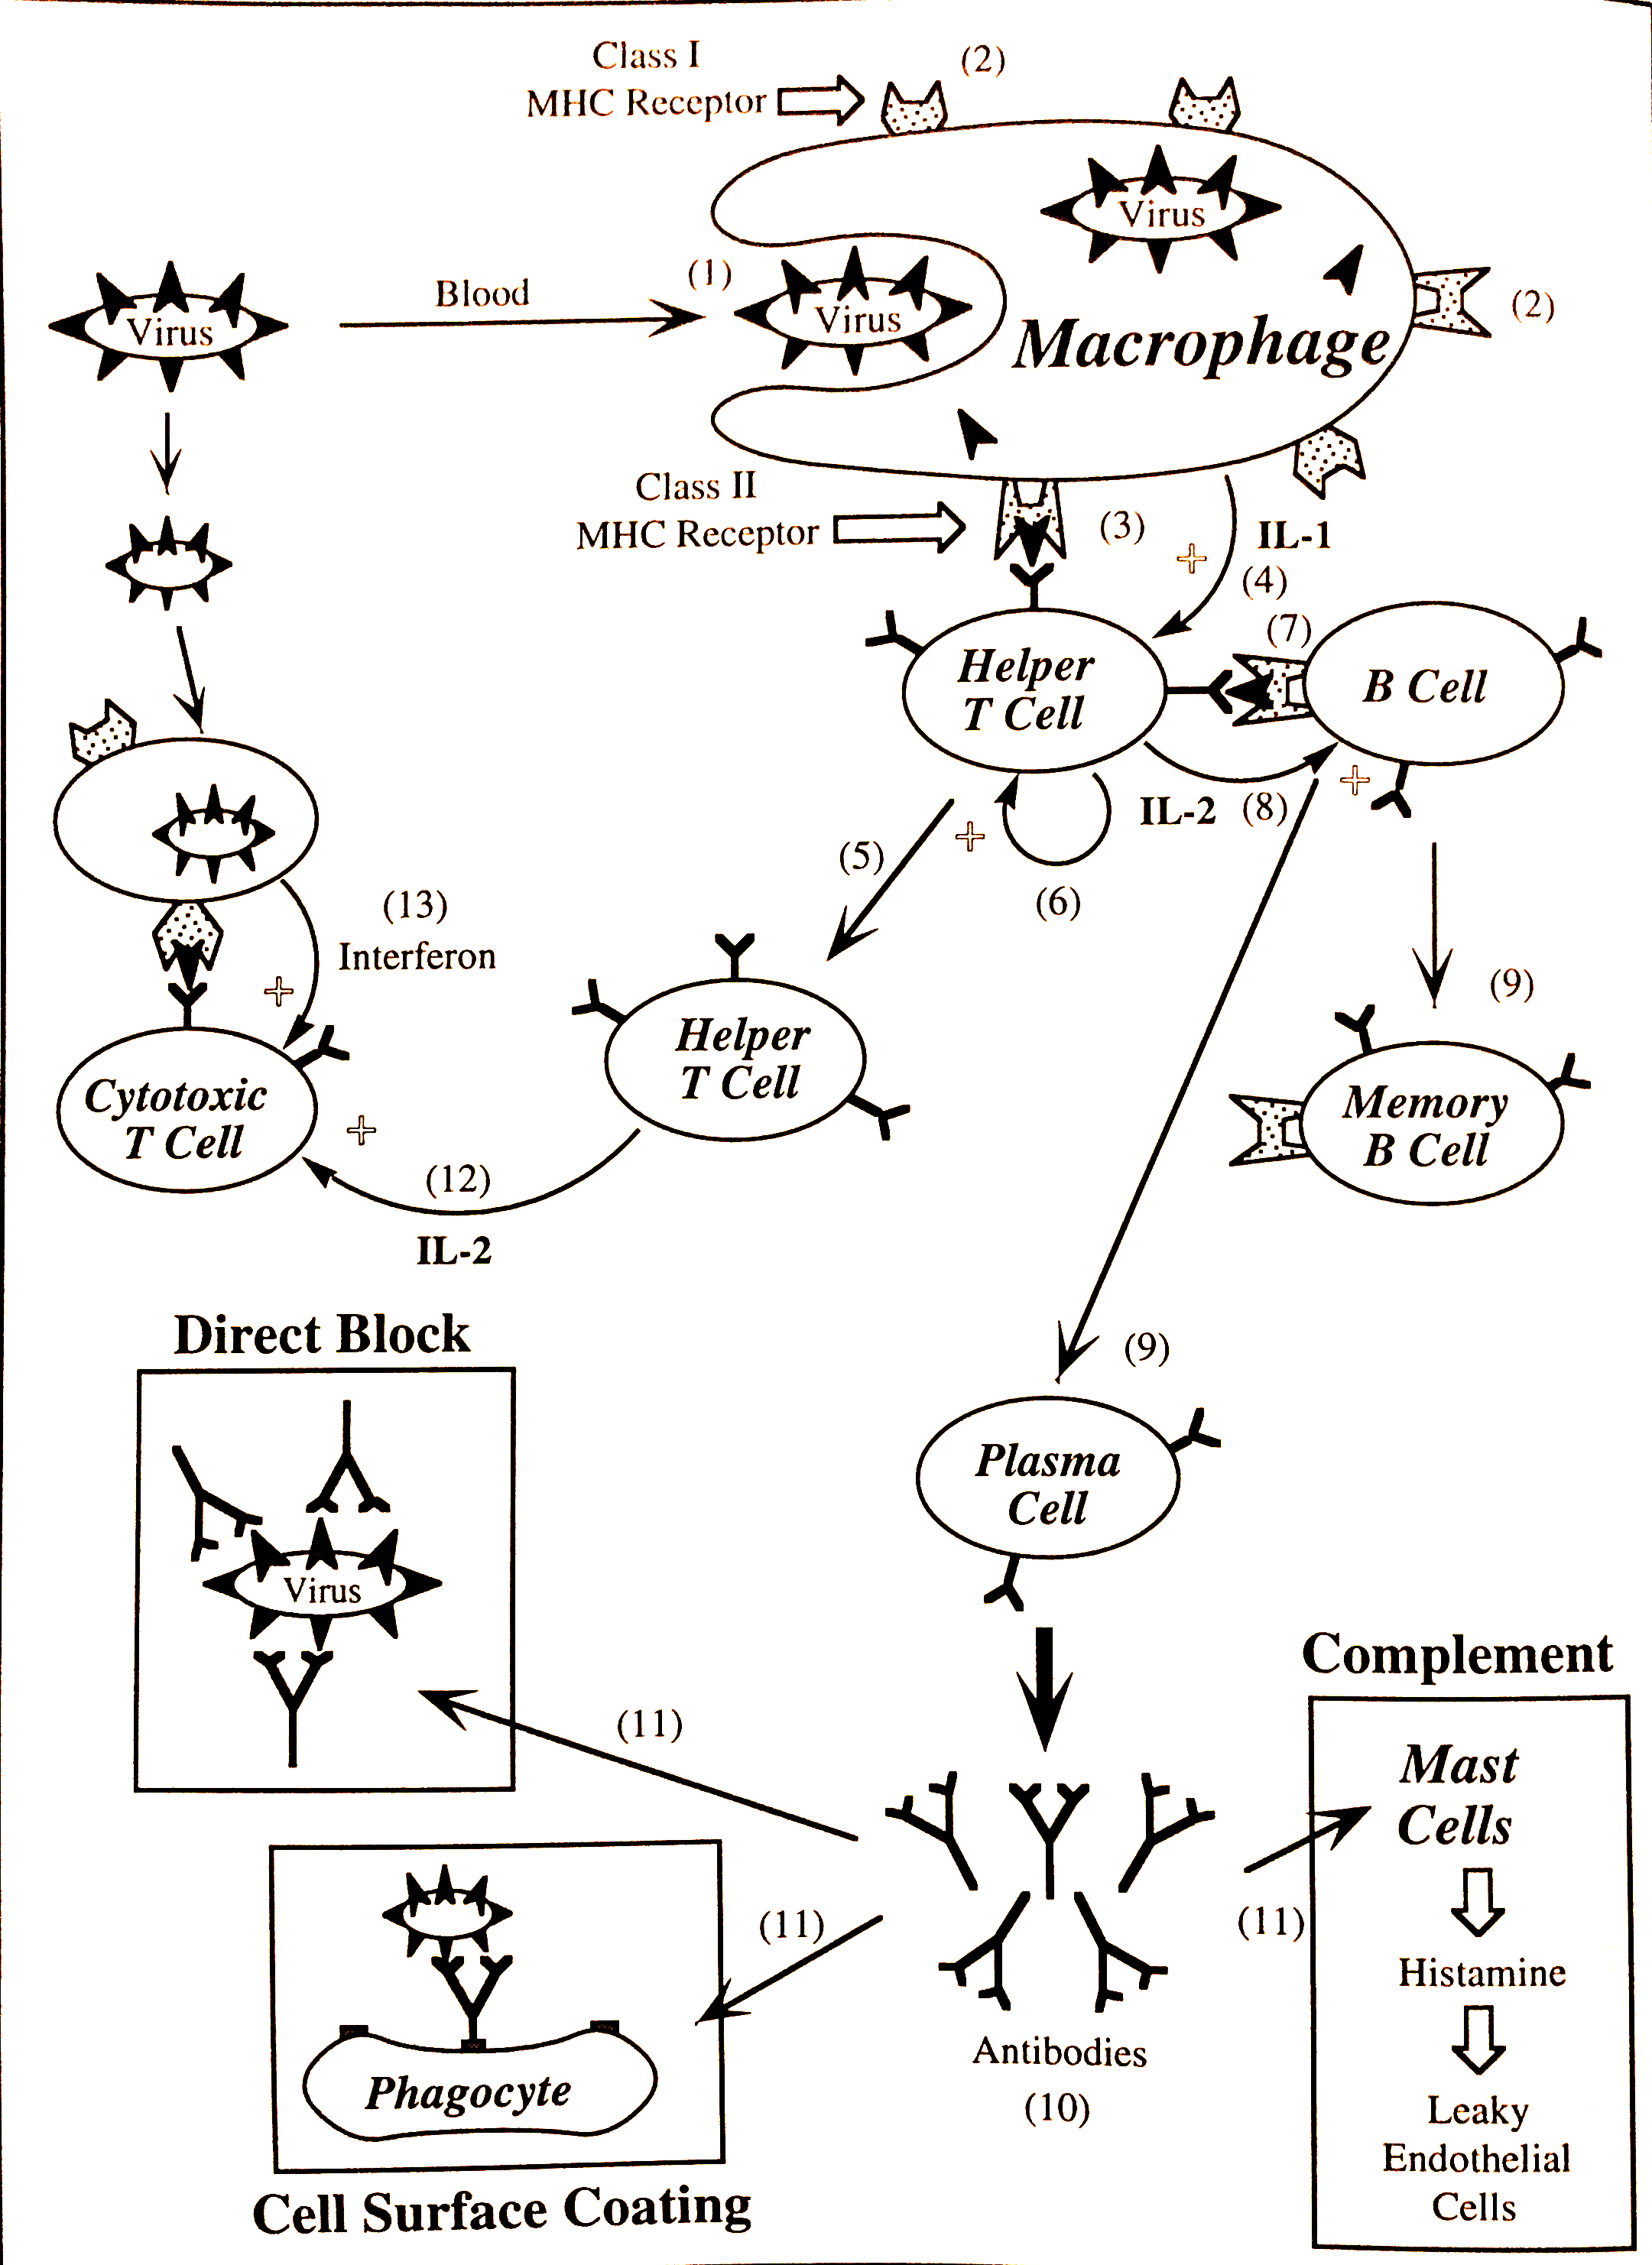
\includegraphics[width=0.7\textwidth]{immune_pathway.png} \label{immune_pathway}
\caption{Review of humoral and cellular immunity pathways.}
\end{figure}

\section{General Chemistry}
\subsection{Stoichiometry}
The MCAT does involve some math, but often it isn't too complicated. Math-related calculations required for MCAT questions involve making approximations, determining ratios, setting up calculations, and estimating the effect of errors on results. Unit conversions to memorize:
\begin{itemize}
	\item Distances: 1 m = 1.094 yd, 2.54 cm = 1 in, 1.609 km = 1 mi
	\item Masses: 1 kg = 2.205 lb, 453.6 g = 1 lb
	\item Volumes: 3.79 L = 1 gal, 1 L = 1.06 qt
	\item Temperatures: $T_F=\frac{9}{5}T_C+32, T_C=\frac{5}{9}\left(T_F-32\right)$
\end{itemize}
\indent \textbf{Molality (m)} is the concentration of a fluid solution defined as the moles of solute per kilogram of solvent. The molality of a solution does not change with temperature, so it is used to calculate the boiling-point elevation and freezing-point depression of solutions containing non-volatile impurities. \textbf{Mass percent} is the concentration of a fluid solution defined as the mass of the solute per mass of solution.\\
\indent Beer's Law is defined to be $\text{Absorbance} = \varepsilon Cl$, where $\varepsilon$ is a constant for the solute at $\lambda_{\text{max}}$ (the wavelength of greatest absorbance), $C$ is the solute concentration, and $l$ is the width of the cuvette. \\
\indent Here are some important solubility rules to remember:
\begin{enumerate}
	\item Most salts containing alkali metal cations (\ce{Li^+}, \ce{Na^+}, \ce{K^+}, \ce{Cs^+}, \ce{Rb^+}) and ammonium (\ce{NH_4^+}) are water-soluble.
	\item Most nitrate (\ce{NO_3^-}) salts are water-soluble.
	\item Most salts containing halide anions (\ce{Cl^-}, \ce{Br^-}, \ce{I^-}) are water-soluble (with heavy metal exceptions such as \ce{Ag^+} and \ce{Pb^2+}).
	\item Most salts containing sulfate anions (\ce{SO_4^{2-}}) are water-soluble (with exceptions such as \ce{Ba^2+}, \ce{Pb^2+}, \ce{Hg^2+}, and \ce{Ca^2+}). 
	\item Most hydroxide anion (\ce{OH^-}) salts are only \textit{slightly} water-soluble. \ce{KOH} and \ce{NaOH} are substantially soluble, while \ce{Ca(OH)_2}, \ce{Sr(OH)_2}, and \ce{Ba(OH)_2} are fairly soluble in water.
	\item Most carbonate anion (\ce{CO_3^{2-}}), chromate anion (\ce{CrO_4^{2-}}), phosphate anion (\ce{PO_2^{3-}}), and sulfid anion (\ce{S^2-}) salts are only slightly water-soluble.
\end{enumerate}
\indent Theres also some general test-taking tips and general advice that could prove very worthwhile:
\begin{enumerate}
	\item Keep in mind that on a multiple-choice exam, the math has been done for you, so all you need to do is approximate the answer.
	\item Intuition will prove useful on the MCAT. As you study for your MCAT, you need to learn to trust your intuition.
	\item Keep in mind that you are \textit{not} graded for showing your work on the MCAT, so don't solve every problem to the last decimal place. Analyze each question only well enough to eliminate three wrong answers. Be concise and efficient in your problem solving, not exhaustive.
\end{enumerate}

\subsection{Atomic Theory}
There are a couple of classical experiments/lab techniques that helped to develop the modern atomic theory that you should be familiar with:
\begin{enumerate}
	\item \textbf{Thomson Experiment:} This experiment helped determine the sign of charges and the charge-to-mass ratio of the electron. Basically, Thomson had a beam of electrons, and showed that he could deflect the beam by applying an electric field by an exact amount each time. The magnitude of deflection depended on the strength of the field, and reversing the plates of the external field got the same magnitude of deflection, but in the opposite direction. Thomson also figured out the charge-to-mass ratio of electrons to by $1.76\times10^8$ C/g, as the arc of deflection was constant in magnitude when the field strength was held constant but its orientation was aligned differently.
	\item \textbf{Millikan Oil Drop Experiment:} This experiment helped determine the the magnitude of charge of subatomic particles. The experimental setup involved trying to suspend a charged oil drop in an electric field. The oil drop became charged by adding an electron to it. The droplet is able to be suspended by balancing the force of gravity with and the force produced by the electric field on the charged oil droplet. Mathematically, this looks like $qE+mg=0$, so $q=-\frac{mg}{E}$. This helped determine the charge on an electron.
	\item \textbf{Rutherford Experiment:} This experiment helped determine the localization of mass/dense particles in an atom. A thin strip of gold foil lies perpendicular to an incoming stream of $\alpha$-particles. The beam strikes the gold strip surrounded by a zinc sulfide \ce{ZnS} band that luminesces if struck by $\alpha$-particles. Rutherford observed that very few $\alpha$-particles ricocheted off the gold, and most passed straight through the gold. This showed that most of an atom was empty space, and that atoms have dense nuclei with nearly all of the atomic mass centrally concentrated. 
	\item \textbf{Mass Spectrometry:} A mass spectrometer is designed to measure the charge-to-mass ratio for a charged particle. This is accomplished by sending a particle into a perpendicular magnetic field and observing the degree to which it curves. By comparing the curvature for an atomic or molecular ion to a known standard, the mass of the unknown ion and/or the mass-to-charge ratio can be determined. This is particularly helpful in determining isotopic abundance. Mathematically, the centripetal force experienced by the particle with mass $m$ is equal to the Lorentz force. Since we are given that the magnetic field $\mathbf{B}$ is always perpendicular to the particle's velocity (with magnitude $v$), this gives us $\frac{mv^2}{r}=qvB$, and solving for $r$ gives $r=\frac{mv^2}{qvB}=\frac{mv}{qB}$. The mass spectrometer embodies a simple concept\textemdash force depends on mass, so when an equal force is applied to different masses, they accelerate at different rates. The mass spectrometer takes advantage of this by accelerating charged particles in motion using a magnetic field. 
\end{enumerate}
\noindent \textbf{Heisenberg's Uncertainty Principle} states that it is not possible to simultaneously know a particle's position and velocity with infinite precision on both. Mathematically, $\Delta x\Delta p\geq \hbar/2$. The \textbf{Bohr Model} describes the transition energy of an electron between two electronic energy levels (principle quantum numbers):
\begin{equation}
\begin{split}
\Delta E=\frac{2\pi^2mZ^2e^4}{h^2}\left(\frac{1}{n_{\text{initial}}^2}-\frac{1}{n_{\text{final}}^2}\right)
\end{split}
\end{equation}
\noindent where $E$ is the energy (principle energy level), $Z$ is the nuclear charge, $n$ is the electronic energy level, $m$ is the mass of an electron, $e$ is the charge of the electron, and $h$ is Planck's constant. The important thing is that excitations (i.e. jumping up to higher energy levels) involve an input of energy, while emissions (i.e. releasing energy by going down to lower energy levels) involve the release of energy. Note also that the energies of the electronic energy levels get closer and closer as you go up. \\
\indent A \textbf{paramagnetic species} (referred to as \textit{radicals} in organic chemistry) is defined as an atom or molecule that contains at least one unpaired electron. The extra electron allows the compound to be responsive to an external magnetic field and `picking up' a magnetic moment, and so can be induced to be magnetic. A \textbf{diamagnetic species} has no unpaired electrons, and so are not susceptible to magnetic fields. Here are some important rules for electronic configurations:
\begin{enumerate}
	\item \textbf{Pauli's Exclusion Principle:} No two electrons can have the same set of quantum numbers.
	\item \textbf{Hund's Rule:} Electrons completely fill lower energy levels before starting to fill higher energy levels. In a degenerate set of orbitals, electrons singly occupy each orbital before a second electron pairs up in the same orbital.
	\item \textbf{Aufbau Principle:} Electrons are added one-by-one to the shells, starting with the lowest energy level, and then into sequentially increasing energy levels. Exceptions occur in the half-filled and filled $d$-shells, which add extra stability. For example, \ce{Cr} (chromium) has \ce{[Ar] 4s^1 3d^5} instead of \ce{[Ar] 4s^2 3d^4}, and \ce{Cu} (copper) has \ce{[Ar] 4s^1 3d^10} instead of \ce{[Ar] 4s^2 3d^9}. 
\end{enumerate}
\noindent The are four types of quantum numbers to know:
\begin{enumerate}
	\item \textbf{Principle ($n$)}: Describes the shell and energy level in which the electron resides. $n\in\mathbb{N}$.
	\item \textbf{Angular Momentum ($l$)}: Describes the orbital in which the electron resides. $l$ is a whole number less than $n$. $l=0$ is an $s$ orbital, $l=1$ is a $p$ orbital, $l=2$ is a $d$ orbital, and $l=3$ is a $f$ orbital.
	\item \textbf{Magnetic ($m_l$)}: Describes the orientation of the orbital about a plane or axis. $-l\leq m_l\leq l$.
	\item \textbf{Spin ($m_s$)}: Describes the rotation (counterclockwise or clockwise) of the electron about its axis. $m_s=\pm 1/2$.
\end{enumerate}
\noindent For $p$-orbitals ($l=1$), $m_l=-1$ corresponds to the $p_x$ orbital, $m_l=0$ corresponds to the $p_y$ orbital, and $m_l=1$ corresponds to the $p_z$ orbital. For $d$-orbitals ($l=2$), $m_l=-2$ corresponds to the $d_{xy}$ orbital, $m_l=-1$ corresponds to the $d_{xz}$ orbital, $m_l=0$ corresponds to the $d_{yz}$ orbital, $m_l=1$ corresponds to the $d_{x^2-y^2}$ orbital, and $m_l=2$ corresponds to the $d_{z^2}$ orbital. \\
\indent The \textbf{coordination number} describes the number of atoms (ligands) attached to a central atom within a molecule. Coordination numbers only count atoms attached, and \textit{not} lone pairs of electrons. For example, \ce{BH_3} has a coordination number of 3.\\
\indent When discussing excitation and relaxation, the generic case is that the energy of the photon absorbed is equal to the energy of the photon emitted. In actuality, there is more than one singular energy level for the ground state and the excited state due to the coupling of electrical energy levels and rotational energy levels associated with the atom. Transitions involve a change in electronic state as well as a change in the rotational energy of the atom. In molecules, there are vibrational energy levels to consider, in addition to the rotational and electronic energy levels. The results is that in actuality, the ground state and excited state exists as a band of energy levels, not a single level. This means that multiple possibilities exist for the energy of transition. Rather than a single line absorption or emission spectrum being formed, a range is formed. \\
\indent The atomic spectrum of hydrogen and its associated energy transitions are well studied. The \textbf{Lyman series} are the transitions that go to the $n=1$ final energy level. The \textbf{Balmer series} are the transitions that go to the $n=2$ final energy level. The \textbf{Paschen series} are the transitions that go the $n=3$ final energy level. The \textbf{Brackett series} are the transitions that go to the $n=4$ final energy level. Of these four series, only the Balmer series emits photons in the visible range. Here is an example problem: 
\begin{center}
\begin{minipage}{30em}
\textcolor{blue}{Given that the wavelength of the emitted light for the $n=3$ to $n=2$ transition in the hydrogen atom is 656 nm, which of the following is NOT true?
\begin{enumerate}[label=\Alph*]
	\item All Balmer series transitions are less than 800 nm.
	\item All Lyman series transitions are less than 400 nm.
	\item The lowest energy Paschen transition is greater than 800 nm.
	\item The highest energy Brackett transition is less than 800 nm.
\end{enumerate}}
\end{minipage}
\end{center}
\noindent Let's consider each of the answer choices one at a time:
\begin{enumerate}
	\item The Balmer series are transitions to the $n=2$ level, and the lowest energy transition is from $n=3$ to $n=2$, and is given to be 656 nm. All other transitions in the Balmer series are more energetic, so these transitions emit photons with a wavelength less than 656 nm. Therefore, choice A is valid.
	\item As a general idea, since we know that $\Delta E\propto\left(\frac{1}{n_i^2}-\frac{1}{n_f^2}\right)$, the transition of $n=2$ to $n=1$ (which is the lowest energy transition in the Lyman series by definition) as at least three times more energy change than the transition of $n=\infty$ to $n=2$. Practically, this means that all photons in the Lyman series are of higher energy and shorter wavelength than the transitions in the Balmer series. A more stringent calculation with $\Delta E=hc/\lambda$ would tell us that indeed, the transitions in the Lyman series emit photons with a wavelength less than 400 nm, meaning that choice B is valid.
	\item The Paschen series involves transitions to the $n=3$ level, and the lowest energy transition in the Paschen series is from $n=4$ to $n=3$, and it is of significantly lower energy than the $n=3$ to $n=2$ transition. This means that the lowest energy photon in the Paschen series is of lower energy and higher frequency than the transitions in the Balmer series. The Balmer series emits a photon at 656 nm, so the lowest energy transition in the paschen series emits a photon with a wavelength greater than 656 nm. Thus, choice C is a valid statment.
	\item The Brackett series involves transitions to the $n=4$ level, and from our above considerations, this should be even less energetic than the Paschen series or Balmer series. Since we showed choice C is valid, the Brackett energy transition cannot be less than 800 nm, so thus choice D is invalid and so choice \textbf{D} is the correct answer.
\end{enumerate}

\subsection{Periodic Trends}
The \textbf{effective nuclear charge} $Z_{eff}$ is the net charge exerted upon the valence electrons, which takes into account the shielding from the core electrons. As you move from left to right across a period in the periodic table, the effective nuclear charge increases. Also, as you descend a family/group in the periodic table, the valence shell increases, so the distance between the atom's valence electrons and its nucleus increases. Periodic trends depend on both $Z_{eff}$ and the valence shell. As you move up the periodic table and to the right, the following general atomic trends are observed:
\begin{enumerate}
	\item The atomic size decreases (the radius of the atom is defined as the distance from the center of the nucleus to the exterior of the valence electron cloud).
	\item The ionization energy increases (the energy required to remove the outermost electron from the atom in its gas phase).
	\item The electron affinity increases (the energetics associated with an atom gaining an electron in its gas phase).
	\item The electronegativity increases (the tendency to hold shared electrons with another atom within a bond). 
\end{enumerate}
\noindent Note that each trend shows some deviation from uniformity, some more than others. The effective nuclear charge does not uniformly increase when we scan left-to-right across a period. Half-filled stability and filled-shell stability cause some of the common deviations seen with electron affinity and ionization energy. For instance, nitrogen has a larger ionization energy than oxygen, because upon ionization, nitrogen loses its half-filled $p$-shell. On the contrary, oxygen gains half-filled stability upon being ionized.\\
\indent As a general rule, cations are smaller than neutral atoms because the loss of electrons allows the atom to compact more tightly. As a general rule, anions are larger than neutral atoms, because the gain of electrons causes the atom to expand given the enhanced repulsion associated with the additional electrons.\\
\indent Helium has a larger \textbf{atomic radius} than hydrogen. This is because the electrons in the $n=1$ level repel one another more than the electrons in any higher quantum level because they have the smallest interelectronic distance. This repulsion forces the electrons away from one another in helium, resulting in a greater area begin occupied by the orbiting electrons, and hence a greater radius for helium. \\
\indent \textbf{Ionization energy} is the energy required to remove a valence electron when the element is in the gas phase. The generic ionization reaction is represented by the equation \ce{E(g) -> E+(g) + e-}, where \ce{E} represents any element. Notable exceptions to the general ionization energy trend occur when there is half-filled stability of the energy level and where there is an $s^2$-shell. In both cases, the ionization energy is higher than expected, and also higher than the ionization energy of adjacent elements in terms of atomic number in most cases we'll be considering. \\
\indent \textbf{Electron affinity} measures the tendency of an element to gain an electron; it can be either negative or positive, meaning that gaining an electron to the valence shell can be either exothermic or endothermic. The generic reaction is represented by the equation \ce{E(g) + e- -> E-(g)}, where \ce{E} represents any element. The biggest deviations are attributed to the stability associated with a filled $s$-shell. For instance, the sudden increase in electron affinity from \ce{Be} to \ce{B}, \ce{Mg} to \ce{Al}, and \ce{Ca} to \ce{Ga} is attributed to the instability of one electron in the $p$-level. No trend for electron affinity is evident in the transition metals. \\
\indent \textbf{Electronegativity} is the ability of an atom to attract towards itself the electrons within a chemical bond. The trend in electronegativity is pretty clean, showing no exceptions at least in the first 20 elements.

\subsection{Important Periodic Families}
All alkali metals are strong reducing agents and react favorably with water in the reaction \ce{2M(s) + 2H_2O(g) -> 2MOH(aq) + H_2(g)}. The oxides they form are variable with the metal. Lithium forms \ce{Li_2O}, sodium forms a peroxide \ce{Na_2O_2}, and potassium, rubidium, and cesium form superoxides \ce{MO_2}. Alkali metals can also be oxidized into cations by halogens, nitrogen, and hydrogen. \\
\indent Alkaline earth metals are not as soluble in water as are the alkali metals in their cation form, primarily due to their \ce{2+} charge and smaller radius. They can react favorably with water (except for Be) according to the reaction \ce{M(s) + 2H_2O(g) -> M(OH)_2(aq) + H_2(g)}. The alkaline earth metals all form oxides \ce{MO} when oxidized by oxygen gas. They can also be oxidized by halogens, nitrogen, and hydrogen.\\
\indent Chalcogens are the sixth group of the periodic table that includes oxygen, sulfur, selenium, tellurium, and polonium. As neutral elements, they are oxidizing agents, but their reactivity decreases as you descend the column. Oxygen exists as a diatomic molecule \ce{O_2}, sulfur and selenium exist as octatomic molecules \ce{S_8} and \ce{Se_8}, and tellurium and polonium exist in vast molecular matrices.\\
\indent Halogens and noble gases are also important but nothing's new here. When exposed to high concentrations of fluorine gas, xenon and krypton are known to form molecular compounds with fluorine. The resulting xenon fluorides and krypton fluorides show more electron density around fluorine than the noble gas, implying that fluorine is more electronegative than either xenon or krypton. Otherwise, noble gases are pretty much unreactive. 

\subsection{Electrochemistry}
Electrochemistry addresses chemical reactions that involve electron transfer. \textbf{Galvanizing} is a protective process that involves plating a more reactive metal onto a less reactive metal, so that this more reactive species (i.e. the \textit{sacrificial metal}) is the one oxidized by air, rather than the material being protected.\\
\indent Generally speaking, organic and biological oxidizing agents are rich in oxygen and poor in hydrogen (e.g. \ce{Na_2CrO_4}, \ce{KMnO_4}, \ce{NAD+}, and \ce{FAD}), and reducing agents are poor in oxygen and rich in hydrogen (e.g. \ce{NaBH_4}, \ce{LiAlH_4}, \ce{NADH}, and \ce{FADH_2}). This is because oxidizing agents get reduced while oxidizing whatever they're reacting with, and reducing agents get oxidized while reducing whatever they're reacting with.\\
\indent The reduction of two protons (\ce{H+}) to form hydrogen gas (\ce{H_2}) is defined as the reference standard, and assigned an \textit{emf} of zero volts. Any compound that can be reduced more favorably than a proton (meaning oxidation is less favorable than a proton) has a positive reduction potential. Likewise, any compound for which reduction is less favorable than a proton (meaning oxidation is more favorable than a proton) has a negative reduction potential. Generally speaking, precious metals do not readily oxidize\textemdash thus, they have relatively high reduction potentials. On the other end of the spectrum are the alkali and alkaline earth metals, which have relatively low ionization energies, so they are easily oxidized, meaning they have negative reduction potentials. Most tables list reduction half-reaction \textit{emf} values, rather than oxidation half-reaction values. \textit{Emf} values do not need to be memorized, but in general, the greater the electron affinity, the greater the reduction potential. Likewise, a lower ionization energy corresponds to a greater oxidation potential (lower reduction potential). \\
\indent The free energy in an electrochemical cell can be described by
\begin{equation}
\begin{split}
\Delta G_{\text{reaction}}=-nF\varepsilon_{\text{cell}}
\end{split}
\end{equation}
\noindent where $F=96500$ C per mole and $n=\text{electrons per reaction}$. A positive electromotive force (cell voltage) is associated with a favorable oxidation-reduction reaction, just as a negative free energy change ($\Delta G$) is associated with a favorable oxidation-reduction reaction. \\
\indent \textbf{Electrochemical cells} convert energy produced in a chemical reaction into electrical current. Oxidation occurs at the anode, meaning that electrons flow away from the anode, and reduction occurs at the cathode (REDCAT), meaning that electrons flow towards the cathode. This means that anions migrate towards the anode and cations migrate towards the cathode through electric fields. The important thing to remember is that \textbf{electrons flow from the anode to the cathode}. There is a standard line notation for cells\textemdash when reading left to right, it goes from anode to cathode, and reactant to product within each half-reaction electrode. For example,
\begin{equation}
\begin{split}
M_{\text{oxidation}} \left(s\right) | yM \text{ } M_{\text{oxidation}}^{2+} \left(aq\right) || zM \text{ } M_{\text{reduction}}^{2+} \left(aq\right) | M_{\text{reduction}} \left(s\right)\\
\text{Reactant in anode } | \text{ Product in anode } || \text{ Reactant in cathode } | \text{ Product in cathode}
\end{split}
\end{equation}
\noindent In general, there are two types of electrochemical cells: \textbf{galvanic cells} (spontaneous cell with $\varepsilon^{\circ}>0$, $\Delta G<0$) and \textbf{electrolytic cells} (non-spontaneous cell with $\varepsilon^{\circ}<0$, $\Delta G>0$, and an applied voltage present to power the cell). Galvanic cells release energy in the form of electrical flow, while electrolytic cells are used for the storage of electrical potential, as is seen when recharging a battery. \\
\indent The \textbf{Nernst equation} is often used to quantify the effect of concentration on the voltage of an electrochemical cell. Mathematically, it is
\begin{equation}
\begin{split}
\varepsilon_{\text{cell}}=\varepsilon^{\circ}-\frac{RT}{nF}\ln Q_{rx}
\end{split}
\end{equation}
\noindent By substituting $R=8.314 \text{J}/\text{mol}\cdot\text{K}$, $T=298$ K, and $F=96500$ C/mol, we get the working equation 
\begin{equation}
\begin{split}
\varepsilon_{\text{cell}}=\varepsilon^{\circ}-\frac{0.059}{n}\log_{10} Q_{rx}
\end{split}
\end{equation}
\noindent where we're being pretty lenient with the units. Note that our working equation has $\log_{10}$ instead of $\ln$ natural logarithm. Here is an example problem using the Nernst equation:
\begin{center}
\begin{minipage}{30em}
\textcolor{blue}{What is the voltage of an electrochemical cell with an anode of zinc metal in 0.01 M \ce{Zn(NO_3)_2} (aq) and a cathode of silver metal in 1.00 M \ce{AgNO_3} (aq)?
\begin{enumerate}[label=\Alph*]
	\item 2.42 V
	\item 2.30 V
	\item 1.62 V
	\item 1.50 V
\end{enumerate}}
\end{minipage}
\end{center}
\noindent First, we must identify the half-reaction:
\begin{equation}
\begin{split}
\text{Oxidation:}\quad \ce{Zn(s)}\rightarrow\ce{Zn^2+}+2\ce{e-}, \quad\quad \ce{Ag+}+\ce{e-}\rightarrow\ce{Ag(s)}
\end{split}
\end{equation}
The standard cell potential for the reaction is found using values from online or a provided table (not the important part here), and we get $\varepsilon^{\circ}=0.80 \text{ V}-\left(-0.76\text{ V}\right)=1.56 \text{ V}$. The actual cell voltage is slightly higher than $1.56$, because there is a higher cation concentration in the cathode than in the anode. The exact value is found using the Nernst equation:
\begin{equation}
\begin{split}
\varepsilon_{\text{cell}}=\varepsilon^{\circ}-\frac{0.059}{n}\log\frac{[\ce{Zn^2+}_{\text{anode}}]}{[\ce{Ag+}_{\text{cathode}}]^2}=1.56\text{ V }-\frac{0.059}{2}\log\frac{0.01}{1^2}=\left(1.56 - 0.03(\log 0.01)\right)\text{ V}=\left(1.56+0.06\right)\text{ V}=1.62 \text{V}
\end{split}
\end{equation}
\noindent giving us the answer choice \textbf{C} as the correct answer, as desired. 

\subsection{Gases and Gas Laws}
The \textbf{collision force} is defined as the force exerted by a gas particle during a collision between it and the container wall. It is based on impulse, so both greater momentum and a shorter time of contact increase the force of impact. The collision force can be increased by increasing the temperature, because greater temperature imparts greater velocity, and thus greater momentum, to each molecule. The \textbf{mean free path} is defined as the average distance a particle can travel before colliding with another particle. There are three key assumptions associated with the \textbf{Kinetic Molecular Theory of Gases}:
\begin{enumerate}
	\item Particles are so small compared to the distances between particles that their volumes are negligible.
	\item Particles move in straight lines, and there are no intermolecular forces. The collisions are said to be elastic with no energy dissipation.
	\item Particles are in constant random translational motion.
\end{enumerate}
\noindent An ideal gas is a theoretical gas that obeys all of these conditions. In a gas system, not all particles have the same kinetic energy\textemdash there is a random distribution of energies defined by the temperature-dependent \textit{Boltzmann distribution}. Of course, no gas is truly ideal, and we have the \textbf{van der Waals equation} to describe real gases:
\begin{equation}
\begin{split}
\left(P_{\text{observed}}+a\frac{n^2}{V^2}\right)\left(V_{\text{container}}-nb\right)=nRT
\end{split}
\end{equation}
\noindent where $a$ is the \textbf{attraction coefficient} ($a>0$ is particles attracting, $a<0$ is particles repelling), $b$ is the `\textbf{bigness coefficient}' ($b>0$ for all particles). Here are two sample problems regarding the van der Waals equation:
\begin{center}
\begin{minipage}{30em}
\textcolor{blue}{Which of the following types of gases has a negative $a$ term?
\begin{enumerate}[label=\Alph*]
	\item Polar
	\item Nonpolar
	\item Hydrophobic
	\item Ionized
\end{enumerate}}
\end{minipage}
\end{center}
\noindent An ionized gas has particles that all have the same charge, and like charges repel, so choice \textbf{D} is the best answer.
\begin{center}
\begin{minipage}{30em}
\textcolor{blue}{Which of the following types of gases has the greatest $b$ term?
\begin{enumerate}[label=\Alph*]
	\item Methane
	\item Ethane
	\item Ethene
	\item Ethyne
\end{enumerate}}
\end{minipage}
\end{center}
\noindent Ethane has the greatest mass of the given molecules, and so it has the greatest $b$ term. Thus, the answer is \textbf{B}. \\
\indent Here's another practice problem, this time regarding how to measure pressure using a manometer and using the equation $\Delta P=\rho g \Delta h$:
\begin{center}
\begin{minipage}{30em}
\textcolor{blue}{What is the pressure in atmospheres of a column of gas in a closed tube above mercury if the height difference at sea level between a connected column of mercury open to the atmosphere and the closed column above mercury is 317 mm?
\begin{enumerate}[label=\Alph*]
	\item 317/760 atm
	\item 443/760 atm
	\item 760/443 atm
	\item 317/443 atm
\end{enumerate}}
\end{minipage}
\end{center}
\noindent The height difference of 317 mm means that the pressure difference is 317 torr (mm Hg, by definition). The atmospheric pressure at sea level is 760 torr, so the gas pressure in the column is $760-317=443$ torr. The conversion from torr to atm involves dividing by a factor of 760 torr per atm, making choice \textbf{B} the best answer. As the question is worded, the pressure difference is provided, but the relative pressure are not mentioned. The pressure could also be $760+317=1077$ torr, but this value is not listed as an answer choice.\\
\indent The \textbf{root mean square speed} of a gas is 
\begin{equation}
\begin{split}
\mu_{\text{rms}}=\sqrt{\frac{3RT}{m}}
\end{split}
\end{equation}
\noindent where $R$ is the ideal gas constant, $T$ is the temperature, and $m$ is the mass of one mole of the gas. This is derived by solving the equation $\frac{1}{2}mv^2=\frac{3}{2}RT$ for $v$, as the left hand side is the kinetic energy from classical mechanics and the right hand side is the energy of the system obtained through the equipartition theorem. Here is an example problem:
\begin{center}
\begin{minipage}{30em}
\textcolor{blue}{What is the root mean square speed of neon atoms at $27^{\circ}$C?
\begin{enumerate}[label=\Alph*]
	\item 19.3 m/s
	\item 211 m/s
	\item 612 m/s
	\item 1018 m/s
\end{enumerate}}
\end{minipage}
\end{center}
\noindent From the periodic table, the mass of one mole of neon is $m=0.20$ kg, and the temperature converted to Kelvin is $T=300$ K. Thus,
\begin{equation}
\begin{split}
\mu_{\text{rms}}=\sqrt{\frac{3RT}{m}}=\sqrt{\frac{3\left(8.314\right)\left(300\right)}{0.020}}=\sqrt{\frac{\left(8.314\right)\left(9\times10^2\right)}{2\times10^{-2}}}\approx \sqrt{\frac{8\times9}{2}\times 10^4}=\sqrt{36\times 10^4}=6\times10^2=600 \text{m/s}
\end{split}
\end{equation}
\noindent where we ignore the units for convenience. Thus, the best answer is choice \textbf{C}. Using this formula for the root mean square speed, we can determine the relative speeds of two gases, giving us \textbf{Graham's law} for gas flow:
\begin{equation}
\begin{split}
\frac{v_2}{v_1}=\sqrt{\frac{m_1}{m_2}}
\end{split}
\end{equation}
\noindent which holds for a given temperature. This equation is basically saying that the speed of the particle is inversely proportional to the square root of its mass, so the lighter the gas, the faster it travels at a given temperature. There is also the relationship
\begin{equation}
\begin{split}
\frac{v_2}{v_1}=\sqrt{\frac{T_2}{T_1}}
\end{split}
\end{equation}
\noindent which holds for a given mass of particles. This is basically saying that the speed of the particle is directly proportional to the square root of the temperature, so the greater the temperature, the faster a gas travels.

\subsection{Phases and Phase Changes}
\textbf{Isochoric} conditions are where the \textit{volume} of the system does not change, and \textbf{adiabatic} conditions are where \textit{heat} nether enters nor exits the system, meaning that the system is perfectly insulated. The \textbf{critical point} is the highest temperature and pressure at which a liquid may be observed. Beyond the critical point, it is impossible to distinguish between a gas and a liquid, so it is referred to as a \textit{supercritical fluid}. The \textbf{triple point} is where all three phases of matter can exist for a given compound. It is also the highest temperature and pressure at which sublimation (and deposition) can occur. Two key facts of water are that its liquid form is denser than its solid form, and it is densest at $4^{\circ}$C. \\
\indent The enthalpy of vaporization is greater in magnitude than the enthalpy of fursion because more energy is necessary to \textit{break} the intermolecular forces (i.e. for liquid $\rightarrow$ gas) than is necessary to weaken the intermolecular forces (i.e. for solid $\rightarrow$ liquid).\\
\indent The formal definition of \textbf{vapor pressure} above a liquid is the force per unit area above the surface of a liquid exerted by molecules formed upon evaporation of the liquid. Vapor pressure can be measured in either an open or closed system. In a closed system, a partial pressure of vapor exists, because the rate of vaporization equals the rate of condensation. This is most typically how vapor pressure is determined. In an open system, since no equilibrium is reached, vapor pressure is a measure of the pressure just above the surface of the liquid. Vapor pressure is \textit{independent} of the shape and volume of a container. Vapor pressure increases as temperature increases, and decreases as the heat of vaporization $\Delta H_{\text{vaporization}}$ increases. The \textbf{Clausius-Clapeyron} equation can be used to explain the relationship between vapor pressure and temperature:
\begin{equation}
\begin{split}
\ln \frac{p_1}{p_2}=\frac{\Delta H_{\text{vaporization}}}{R}\left(\frac{1}{T_2}-\frac{1}{T_1}\right)
\end{split}
\end{equation}
\noindent The conclusion from this is that as the temperature of a liquid increases, the pressure of its vapor increases in an exponential manner. This equation assumes that the heat of vaporization $\Delta H_{\text{vaporization}}$ is constant over the temperature range of interest. Detailed calculations involving the Clausius-Clapeyron equation are unlikely, but it should still be understood conceptually and graphically.\\
\begin{equation}
\begin{split}
\text{As } \Delta H_{\text{vaporization}}\uparrow; \text{ Volatility } \downarrow; \text{ Boiling Point } \uparrow; \text{ Vapor Pressure} \downarrow
\end{split}
\end{equation}
\noindent The \textbf{boiling point} is defined as the temperature at which the vapor pressure is equal to the atmospheric pressure. According to \textbf{Raoult's Law}, the vapor pressure above a solution of two or more \textit{miscible} liquids depends on the mole fraction of each compound in solution. Mathematically,
\begin{equation}
\begin{split}
P_{\text{vapor}}=\xi_iP_{\text{vapor (pure)}}
\end{split}
\end{equation}
\noindent where the $\xi_i$ in Raoult's equation is the mole fraction of the component \textit{in solution}, not in the vapor state. With real compounds, because of intermolecular forces within liquids, there are other factors that come into play. The molecules interact in both the liquid and gas phases, so the vapor pressure relationship is not \textit{exactly} linear as Raoult's equation approximates it to be. Intermolecular forces are greater in the solution than the gas phase. If there is an overall increase in attractive forces in solution whent he components are mixed, then vaporization, and thus vapor pressure, decreases, resulting in a negative deviation from linearity. Likewise, if there is an overall decrease in attractive forces in solution when the components are mixed, then vaporization, and thus vapor pressure, increases, resulting in a positive deviation from linearity. \textbf{Distillation} is removing a liquid from a solution by utilizing their differing vapor pressures/boiling points. 

\subsection{Colligative Properties}
Colligative properties are properties of a solution that are affected by the concentration of a soluble impurity. Colligative properties include boiling point elevation, freezing point depression, and osmotic pressure. The electrical conductivity of a solution, although it is not formally a colligative property, shows a dependence on ion concentration. The increase in boiling point $\Delta T_b$ when solute is added to a solution is given by
\begin{equation}
\begin{split}
\Delta T_b=k_b\cdot i\cdot m
\end{split}
\end{equation}
\noindent where $i$ is the number of ions that form upon dissolving, $m$ is the \textit{molality} of the solution, and $k_b$ is a constant for the solvent. Similarly, we also have the equation for freezing point depression which basically looks that same as that for boiling point elevation:
\begin{equation}
\begin{split}
\Delta T_f=k_f\cdot i\cdot m
\end{split}
\end{equation}
\noindent Note that $\Delta T_f<0$ and $\Delta T_b>0$ (that's why its called freezing point \textit{depression} and boiling point \textit{elevation}).\\
\indent Water has a natural tendency to flow from solutions of higher water concentration (i.e. lower solute concentration) to solutions of lower water concentration (i.e. higher solute concentration) to reach equal concentrations. Pressure differences cause fluids like water to flow, and the driving force causing water to flow is known as \textbf{osmotic pressure}. Osmotic pressure $\pi$ is the pressure exerted by a solution through osmosis across a semipermeable membrane, and is given by
\begin{equation}
\begin{split}
\pi=MiRT
\end{split}
\end{equation}
\noindent where $M$ is the \textit{molarity}, $i$ is the number of ions upon dissociation, $R$ is the ideal gas constant, and $T$ is the temperature. The \textbf{condosity} of a solution is defined as the molar concentration of an aqueous sodium chloride solution that has the same specific conductance as the aqueous salt solution. 

\subsection{Solubility}
A \textbf{supersaturated} solution is where the amount of solute that is dissolved into solution is beyond the maximum amount at that given temperature. The solution is actually a suspension that when disturbed can form a precipitate rapidly. This state can be achieved by first heating a solvent, then adding solute to the solution until the solution is saturated at that temperature. Slowly cooling this solution causes the amount of solute in it to exceed that should dissolve at the reduced temperature. \textbf{Gram solubility} is the quantitative measurement of the maximum number of grams of solute that can dissolve into enough solvent to make one hundred mL of solution under ambient conditions. Here are the solubility rules you should know:
\begin{enumerate}
	\item Most salts composed of +1 cation (excluding transition metals) and -1 anion are soluble in water at room temperature. Nitrate \ce{NO_3-} salts are water-soluble.
	\item Most salts containing sulfate \ce{SO_4^{2}-} anions \textit{with +1 cations} (excluding transition metals) are water-soluble.
	\item Most salts with -2 or -3 anions are insoluble in water (excluding sulfate salts).
	\item Most oxide \ce{O^{2}-} and hydroxide \ce{OH-} anion salts are only slightly water soluble. \ce{KOH} and \ce{NaOH} are notable exceptions that are substantially water soluble. 
\end{enumerate}
\noindent An \textbf{ion-exchange} column exchanges one ion in solution for another (which is initially bound to the column), by precipitating out the ion that forms the less soluble salt and releasing a more soluble into solution to replace it. A water softener is a good example of an ion-exchange column\textemdash hard water (rich in \ce{Ca^{2}+(aq)}) travels down the column where the anion in the ion-exchange resin binds calcium cations to form an insoluble salt while releasing sodium cations \ce{Na+(aq)} into solution. Aqueous sodium cation is referred to as soft water. As calcium precipitates through the column, it is filtered from the water, preventing it from forming precipitates in the plumbing lines of appliances. The reaction that we're interested in is \ce{2Na+(aq) + CaCl_2(s) <-> Ca^{2}+(aq) + 2NaCl (s)}; this reaction highly favors the reactants side. There's also another thing called \textbf{selective precipitation and ion exchange}, where we add an ion to solution with the intention of precipitating an existing ion out of the solution. This is basically the same thing as the ion-exchange column, and can be achieved when the salt being precipitated is less soluble than any other salt combination in solution. For example, consider the reaction \ce{2AgCl(s) + Hg^{2}+(aq) <-> 2Ag+(aq) + HgCl_2(s)}. Because mercury chloride is less soluble than silver chloride, the addition of silver chloride to the mercury solution precipitates mercury out of water.\\
\indent When reactions are added together, the equilibrium constant $K$ fot eh overall reaction is the product of the equilibrium constants of the component reactions. Here is an example problem for solubility:
\begin{center}
\begin{minipage}{30em}
\textcolor{blue}{Silver chloride \ce{AgCl} is MOST soluble in which of the following solutions at $25^{\circ}$C?
\begin{enumerate}[label=\Alph*]
	\item 0.10 M \ce{HgNO_3(aq)}
	\item Pure water
	\item \ce{AgNO_3(aq)}
	\item \ce{NaCl}
\end{enumerate}}
\end{minipage}
\end{center}
As discussed above, silver chloride is most soluble in a solution where \ce{Hg+(aq)} is present, as the mercury ion in solution can bind the chloride anion to form a precipitate. As the amount of \ce{Cl-} in solution decreases as a result, more \ce{AgCl} dissolves into solution to replace it. Thus, the best answer is choice \textbf{A}. Both choices C and D are eliminated because of the common ion effect. 

\subsection{Acids and Bases}
The \textbf{haloacids} are the series of \ce{HX} acids, where \ce{X} represents a halogen. As the size of the halogen increases, the haloacid becomes more acidic due to the increased stability of the conjugate base halide as it increases in size. Dissociation increases, bond strength decreases, and bond length increases as \ce{X} gets bigger. \\
\indent Within a period of the periodic table, it is electronegativity that dictates the strength of an acid, \textit{not} atomic radius. A prime example of this idea is the relationship between ammonia \ce{H-NH_2}, water \ce{H-OH}, and hydrofluoric acid \ce{H-F}. The strongest acid of the three is \ce{HF}, because fluorine is more electronegative than oxygen or nitrogen. The atomic size doesn't change that noticeably between the three elements\textemdash the periodic trend that changes the most from \ce{N} to \ce{F} is the electronegativity.\\
\indent To determine how much acid (or base) is necessary to neutralize a solution of base (or acid), use $M_1V_1=M_2V_2$. Make sure to take into account if the acid is polyprotic/the base has multiple hydroxide groups or something like that. Here is an example problem:
\begin{center}
\begin{minipage}{30em}
\textcolor{blue}{Citric acid (\ce{C_6H_8O_7}) has three dissociable protons with \ce{pK_a} values of 3.14, 4.79, and 5.20. Which of the following solutions would have the lowest pH value?
\begin{enumerate}[label=\Alph*]
	\item 50 mL 0.10 M citric acid (aq) + 75 mL 0.20 M \ce{NaOH(aq)}
	\item 25 mL 0.10 M citric acid (aq) + 50 mL 0.10 M \ce{NaOH(aq)}
	\item 25 mL 0.20 M citric acid (aq) + 75 mL 0.20 M \ce{NaOH(aq)}
	\item 50 mL 0.20 M citric acid (aq) + 50 mL 0.10 M \ce{NaOH(aq)}
\end{enumerate}}
\end{minipage}
\end{center}
\noindent The lowest pH belongs to the solution that is most acidic, and the most acidic solution is the one where the fewest equivalents of base relative to citric acid have been added. In choice D, the \ce{NaOH(aq)} solution is of equal volume and half the concentration of the citric acid solution, so there is only one-half of an equivalent of \ce{NaOH(aq)}. Comparing this with the other answer choices, this is the lowest number of equivalents of the base compared to the other answer choices, so thus, choice \textbf{D} is the best answer.\\
\indent In a solution, the distribution within a conjugate pair is dictated by the pH of the solution. The conjugate pair favors the conjugate acid form in the presence of hydronium, and favors the conjugate base form in the presence of hydroxide. In general, if pH>pK\textsubscript{a}, the solution is basic relative to the compound, so it exists predominantly in its deprotonated form (\ce{[A-]}>\ce{[HA]}). If pH<pK\textsubscript{a}, the solution is acidic relative to the compound, so it exists predominantly in its protonated form (\ce{[A-]}<\ce{[HA]}). 
\begin{center}
\begin{minipage}{30em}
\textcolor{blue}{What is the pK\textsubscript{a} for ammonia \ce{NH_3}, given that the pK\textsubscript{b} for ammonia is 4.7?
\begin{enumerate}[label=\Alph*]
	\item 4.7
	\item 7.0
	\item 9.3
	\item 33
\end{enumerate}}
\end{minipage}
\end{center}
\noindent \textbf{It is not 9.3!} The compound with a pK\textsubscript{a} of 9.3 is ammonium (\ce{NH_{4}+}), the conjugate acid of ammonia. Ammonia is a weaker acid than ammonium, so it has a pK\textsubscript{a} greater than 9.3. The best answer is 33, choice \textbf{D}, indicating that ammonia is such a weak acid that when added to water, there is no detectable dissociation. The mistake of choosing 9.3 is easy to make, one that most students make routinely. However, the equation pK\textsubscript{a, (HA)}+pK\textsubscript{b (A\textsuperscript{-})}=14 is for conjugate pairs, not for the same compound. The pH of a solution composed of both components in a weak conjugate pair can be determined using the \textbf{Henderson-Hasselbalch} equation:
\begin{equation}
\begin{split}
\ce{pH}=\ce{pK_a}+\log\frac{\ce{[HA]}}{\ce{[A-]}}
\end{split}
\end{equation}
\noindent The equation shows that as the conjugate base concentration \ce{[HA]} increases, the pH of the buffer increases.

\subsection{Titration Curves}
A \textbf{buffer} is a solution whos pH remains relatively constant after the addition of either strong acid or strong base. The pH may vary slightly, but for all intents and purposes, it does not change significantly. The pH of a buffered solution is determined using the Henderson-Hasselbalch equation, as discussed in the previous section. Buffers are made of a roughly equal mole mixture of a weak acid and its weak conjugate base in an aqueous solution. The pH range of a buffer is pH$\in[\text{pK\textsubscript{a}}-1, \text{pK\textsubscript{a}}+1]$. Buffers can be made by mixing any of the following things together:
\begin{enumerate}
	\item Weak acid + the salt of the conjugate base in roughly equal mole proportions (e.g. \ce{HCO_2H} with \ce{HCO_2Na}). 
	\item Weak base + the salt of the conjugate acid in roughly equal mole proportions (e.g. \ce{NH_3} with \ce{NH_4Cl}).
	\item Weak acid + roughly half of an equivalent of strong base (e.g. \ce{HOAc} with a half-equivalent of \ce{KOH}).
	\item Weak base + roughly half of an equivalent of strong acid (e.g. \ce{H_3CNH_2} with a half-equivalent of \ce{HCl}).
\end{enumerate}
\noindent Physiological pH is considered to be 7.4 and is usually highly buffered in most regions of the body. In a \textit{titration}, the \textbf{equivalence point} is reached when the moles of acid are equal to the moles of base.\\
\indent A typical acid-base \textbf{indicator} is an organic acid with extended conjugation. Its weak acid and conjugate weak base have two distinct colors. The energy state transition that produces color involves the $\pi$-bonding and $\pi$-antibonding orbitals, and depends on the electron-donating and electron-withdrawing nature of the substituents on the $\pi$-system.  
\hilight{TODO} %TODO

\subsection{Equilibrium}
The \textbf{equilibrium constant} $K_{eq}$ is a mathematical quantity that is calculated for a reaction at equilibrium. By definition, the equilibrium constant is the concentration of products at equilibrium divided by the concentration of reactants at equilibrium. Stoichiometric values from the balanced equation become exponents in the $K_{eq}$ expression. Do \textit{not} include solids or pure liquids in the $K_{eq}$ expression, only solutes (for $K_c$) and gases (for $K_p$). The numerical value of $K_{eq}$ varies only with changing temperature, not with catalysts, pressure, volume, or moles. Equilibrium constants are unitless by definition. All equilibrium constants obey the same rules, but depending on the reaction, there may be special features that recur. Different reactions have special $K$ values.\\
\begin{table}[!ht]
\arraycolsep=1.4pt\def\arraystretch{1.5}
\begin{tabular}{|l|l|}
\hline
\textbf{$K$ Type}    & \textbf{Type of Reaction to Which the $K$ Applies} \\ \hline
$K_p$      & $K_{eq}$ for reaction of gases. Values are in \textit{pressure} units. \\ \hline
$K_c$       & $K_{eq}$ for reaction of solutes. Values are in \textit{concentration} units. \\ \hline
$K_{sp}$     & $K_{eq}$ for salts dissociating into ions. Measures the \textit{solubility}. \\ \hline
$K_{a}$   & $K_{eq}$ for acids dissociating into water. Measures the \textit{acidity}. \\ \hline
$K_{b}$    & $K_{eq}$ for bases dissociating in water. Measures the \textit{basicity}. \\ \hline
$K_w$     & $K_{eq}$ for autoionization of \textit{water} into \ce{H+} and \ce{OH-}. \\ \hline
\end{tabular}
\end{table}
\indent A \textbf{complex equilibrium} is a balance between two separate reactions that share a common reagent or set of reagents. In essence, it is two reactions who equilibrium states depend on one another. Here is an example of a complex equilibrium: 
\begin{center}
\begin{minipage}{30em}
\textcolor{blue}{Consider the following complex equilibrium. When \ce{N_2O_4} gas is removed, how are the partial pressures of \ce{NO} gas and \ce{NO_2} gas affected?
\begin{equation}
\begin{split}
\ce{2NO(g) + O_2(g) <-> 2NO_2(g)}, \quad K_{eq1}\\
\ce{2NO_2(g) <-> N_2O_4(g)}, \quad K_{eq2}\\
\hline\\
\ce{2NO(g) + O_2(g) <-> N_2O_4(g)}, \quad K_{eq1}\times K_{eq2}
\end{split}
\end{equation}
\begin{enumerate}[label=\Alph*]
	\item $P_{\ce{NO}}$ and $P_{\ce{NO_2}}$ both decrease.
	\item $P_{\ce{NO}}$ and $P_{\ce{NO_2}}$ both increase.
	\item $P_{\ce{NO}}$ decreases, while $P_{\ce{NO_2}}$ remains the same.
	\item $P_{\ce{NO}}$ increases, while $P_{\ce{NO_2}}$ remains the same.
\end{enumerate}}
\end{minipage}
\end{center}
\noindent The second reaction shifts to the right to compensate for the loss of \ce{N_2O_4}, so the partial pressure of \ce{NO_2} decreases. In turn, a decrease in \ce{NO_2} causes the first reaction to shift to the right as well, resulting in a decrease in the partial pressure of \ce{NO} gas and an increase in the partial pressure of \ce{NO_2}. However, this increase in \ce{NO_2} from the forward shift of the first reaction is less significant than the decrease in the \ce{NO_2} caused by the forward shift of the second reaction. This is because the shift in the first reaction cannot completely replenish the lost \ce{NO_2} without losing so much \ce{NO} that the reaction is beyond equilibrium. A shift \textit{never} regenerates as much as was lost. Both \ce{NO} and \ce{NO_2} this decrease, making choice \textbf{A} the best answer. \\
\indent Equilibrium is \textbf{dynamic}, meaning that it is a state where the system is continually reacting in both the forward and reverse directions, even though no net change is observed at the macroscopic level. \textbf{Le Ch\^atelier's Principle} says that if an external stress is applied to a system at equilibrium, the system will shift itself in such a way that the stress is partially relieved as best as possible and equilibrium is re-established. To see this in action, consider the reaction \ce{N_2O_4 <-> 2NO_2(g)}, which is an endothermic reaction with $\Delta H = +146$ kJ/mole:
\begin{enumerate}
	\item If \ce{N_2O_4(g)} is added, the system shifts to the right.
	\item If \ce{NO_2(g)} is added, the system shifts to the left.
	\item If the external pressure is increased, the system favors the side with less molecules to reduce the increased crowding, thus shifting the system to the left.
	\item If the volume is increased, the system is less crowded and molecules collide less often, so the system shifts to the right.
	\item If the system is heated, this gives a net influx of energy, shifting the \textit{endothermic} system to the right.
	\item If the system is cooled, the system wants to produce energy to compensate, shifting the system to the left.
\end{enumerate}

\subsection{Thermochemistry}
\textit{Exergonic} means $\Delta G<0$, while \textit{exothermic} means $\Delta H<0$. Similarly, \textit{Endogonic} means $\Delta G>0$, while \textit{endothermic} means $\Delta H>0$. The standard free energy change $\Delta G^{\circ}$ is the free energy change when a reaction goes from standard conditions to equilibrium. Standard conditions are defined as 1 atm of pressure and a temperature of 298 K, and all solute species (reactants and products) present at 1.00 M concentration. We have
\begin{equation}
\begin{split}
\Delta G^{\circ} = -RT\ln K_{eq}
\end{split}
\end{equation}
\noindent If we don't start at reaction quotient $Q=1$ by not having all the solute species at 1.00 M concentration, then the adjusted free energy change is
\begin{equation}
\begin{split}
\Delta G_{\text{rxn}}=RT\ln\frac{Q_{\text{rxn}}}{K_{eq}}
\end{split}
\end{equation}

\subsection{Chemical Kinetics}
The \textbf{order} of a reaction is ascertained from the number of reagents involved in the rate-determining step. There are three fundamental reaction orders to consider: zero, first, and second. 
\begin{table}[!ht]
\arraycolsep=1.4pt\def\arraystretch{1.5}
\begin{tabular}{|l|l|l|l|}
\hline
                      & \textbf{Zero Order} & \textbf{First Order} & \textbf{Second Order} \\ \hline
\textbf{Rate Law:}    & $\text{Rate}=k$                   & $\text{Rate}=k[A]$                    & $\text{Rate}=k[A]^2$                     \\ \hline
\textbf{Half-Life:}   & $t_{1/2}=\frac{[A]_0}{2k}$                   & $t_{1/2}=\frac{\ln 2}{k}=\frac{0.693}{k}$                    & $t_{1/2}=\frac{1}{k[A]_0}$                     \\ \hline
\textbf{Rate:} & Constant rate                   & Rate $\downarrow$ as time $\uparrow$              & Rate $\downarrow$ as time $\uparrow$                     \\ \hline
\textbf{Half-Life:} & Half-life $\downarrow$ as time $\uparrow$ & Half-life constant & Half-life $\downarrow$ as time $\downarrow$ \\ \hline
\end{tabular}
\end{table}
\indent The rate of a reaction is affected by several factors such as temperature, activation energy, catalysts, solvent (solvents affect the stability of the transition state), collision frequency, collision orientation, and the concentration of the reactants in the rate-determining step. The rate constant $k$ must account for all of these factors, except concentration of the reactants, and is given by
\begin{equation}
\begin{split}
k=A\exp\left(\frac{-E_{\text{activation}}}{RT}\right)
\end{split}
\end{equation}
\noindent where $A$ is the Arrhenius constant\textemdash it takes into account collision orientation and frequency. Because half-life is constant for first-order processes, most half-life questions on the MCAT involve decay (a first-order reaction), which can be described by
\begin{equation}
\begin{split}
C_t=C_0e^{-kt}
\end{split}
\end{equation}
\noindent where $C_t$ is the concentration at time $t$, $C_0$ is the initial concentration, $t$ is time, and $k$ is the rate constant. The half-life of decay is $t_{1/2}=\left(\ln 2\right)/k\approx 0.693/k$.\\
\indent In nuclear chemistry, a heavy element undergoes a decay process (i.e. fission) to increase its nuclear stability. A light element undergoes a capture process (i.e. fusion) when struck by a high-energy particle to increase its nuclear stability. 
\begin{table}[!ht]
\arraycolsep=1.4pt\def\arraystretch{1.5}
\begin{tabular}{|l|l|}
\hline
\textbf{Process}    & \textbf{Reaction Tracking} \\ \hline
$\alpha$-Decay      & \ce{{}^{120}_{50}X -> {}^{4}_{2}$\alpha$ + {}^{116}_{48}Y} \\ \hline
$\beta$-Decay       &  \ce{{}^{120}_{50}X -> {}^{0}_{-1}e + {}^{120}_{51}Z} \\ \hline
$\beta^+$-Decay     & \ce{{}^{120}_{50}X -> {}^{0}_{1}e + {}^{120}_{49}Q} \\ \hline
$\gamma$-Emission   & \ce{{}^{120}_{50}X^* -> h$\nu$ + {}^{120}_{50}X} \\ \hline
$\alpha$-Capture    & \ce{{}^{120}_{50}X + {}^{4}_{2}$\alpha$ -> {}^{124}_{52}A} \\ \hline
$\beta$-Capture     & \ce{{}^{120}_{50}X + {}^{0}_{-1}e -> {}^{120}_{49}Q} \\ \hline
$\beta^+$-Capture   & \ce{{}^{120}_{50}X + {}^{0}_{1}e -> {}^{120}_{51}Z} \\ \hline
$\gamma$-Absorption & \ce{{}^{120}_{50}X + h$\nu$ -> {}^{120}_{50}X^*} \\ \hline
\end{tabular}
\end{table}

\section{Organic Chemistry of Biological Systems}
\subsection{Molecular Structure}
For nonpolar $\sigma$ bonds, most of the electron density is \textit{between} the nuclei. This means that when drawing electron cloud diagrams, the $\sigma$ bond looks more like an ellipsoid as opposed to a dumbbell.\\
\indent The more substituted a carbon atom is, the less strong bonds it is able to form. This is because the other groups are able to (mildly) take electrons away from the bond of interest and thus make it weaker. Bonds involving $sp^3$ carbons are the weakest, while those involving $sp$ carbons are the strongest, because they have the most $s$ character. And of course, triple bonds are the strongest, while single bonds are the weakest, because of the number of electrons shared between atoms. For example, consider the molecule shown in Figure \ref{oc:1.4}.
\begin{equation}
\begin{split}
\chemfig{
           \mcfatomno{1}% 1
    -[:320]\mcfatomno{2}% 2
              (
        -[:260]\mcfatomno{13}% 13
                  (
            -[:320]\mcfatomno{15}% 15
                  )
        -[:200]\mcfatomno{14}% 14
              )
     =[:20]\mcfatomno{3}% 3
              (
         -[:80]\mcfatomno{5}% 5
              )
    -[:320]\mcfatomno{4}% 4
              (
        <[:260]H\mcfatomno{6}%\mcfright{H}{\mcfatomno{6}}% 6
              )
              (
       <:[:220]\mcfatomno{7}% 7
              )
     -[:10]\mcfatomno{8}% 8
              (
        <:[:60]H\mcfatomno{9}%\mcfright{H}{\mcfatomno{9}}% 9
              )
              (
      -[:287.5]\mcfatomno{11}% 11
              )
     <[:25]\mcfatomno{10}% 10
    -[:325]\mcfatomno{12}% 12
}
\end{split} \label{oc:1.4}
\end{equation}
Here, let us consider Bonds A (1 and 2), B (2 and 3), C (2 and 13), and D (4 and 8). Between these four bonds, B is the strongest since it is a double bond. D is the weakest because it is between two $sp^3$-hybridized carbons. Bond A is stronger than bond C, despite both sharing an $sp^2$-hybridized and $sp^3$ hybridized carbon, because bond C contains the more highly substituted carbon.\\
\indent Hybridization of carbon atoms can affect the acidity of hydrogens bound to them. Contrary to most other acids, as the hybrid orbital gets smaller, the electrons are held closer to the nucleus of the atom boned to hydrogen, so the bond can be cleaved in a heterolytic fashion more easily. The more $s$-character in the hybrid orbital of the atom bonded to the hydrogen, the stronger the acid. This results in the relative acidity being $sp>sp^2>sp^3$. This trend is most commonly observed with \ce{C} acidity, but can also be observed with \ce{N} and \ce{O}.\\
\indent Steric hindrance occurs any time two atoms attempt to be in the same place at the same time. It is repulsive in nature and increases as the atoms draw closer. On cyclohexane, substituents with axial orientation experience greater steric hindrance than substituents with equatorial orientation. Thus, substituents (especially the bulky ones) prefer to be in the equatorial position.\\
\indent \textit{Intermolecular forces are the primary consideration} when approximating physical properties (i.e. boiling point). If IMFs are not enough, you also need to consider the molecular mass and molecular rigidity of the molecules. Heavier compounds have higher boiling points, and compounds with greater molecular flexibility can twist and conform to allow for more surface area, and thus more intermolecular interactions. This is why cell membranes would be most rigid if their fatty acids were completely saturated and long molecules, as interactions are greatest with long, saturated fatty acids. \\
\indent The best micelles has an ionic (charged) head and a long carbon chain for the organic tail. For example, \ce{H_3C(CH_2)_{14}CO_2^-} is a better micelle than \ce{H_3C(CH_2)_{14}CO_2H} because it has a charged head, which is more hydrophilic than even the polar, protic carboxylic acid.\\
\indent The inductive effect can be applied to both electron withdrawal (i.e. with the canonical example of nearby halogens) and electron donation. For instance, methyl amine is more nucleophilic than ammonia (\ce{NH_3}) because the methyl group is electron-donating. Varying the $R$-group changes the inductive effect. It also changes the size of the molecule, so steric hindrance can affect the reaction. For instance, \ce{(H_3C)_3N} is less nucleophilic than \ce{(H_3C)_2NH} because the electron donation by the additional methyl group does not compensate for the increase in molecular size.\\
\indent Stereochemistry prefixes, to denote orientation:
\begin{itemize}
\item \textbf{R vs. S} R is clockwise around a stereocenter, S is counterclockwise. This convention is used for chiral centers.
\item \textbf{E vs. Z} E is high priority groups on opposite sides of the double bond. Z is high priority groups are on the same side of the double bond. This convention is used for double bonds.
\item \textbf{$\alpha$ vs $\beta$} $\alpha$ means that the hydroxyl group attached to \ce{C_1} (atom 8 in Figure \ref{oc:2} for both molecules) and the \ce{-CH_2OH} group at \ce{C_5} (the groups on atoms 2 and 10 in Figure \ref{oc:2} for both molecules) lies on opposite sides of the ring's plane (a \textit{trans} arrangement), while $\beta$ means that they are on the same side of the plane (a \textit{cis} arrangement). This convention is used when discussing the glycosidic bond between sugar molecules. 
\end{itemize}
\begin{equation}
\begin{split}
\chemfig{
            \mcfatomno{15}O% 15
    >:[:330]\mcfatomno{14}% 14
      -[:30]\mcfatomno{13}% 13
               (
          <[:90]O\mcfatomno{16}% 16
               )
     -[:330]\mcfatomno{12}% 12
               (
         <:[:30]O\mcfatomno{17}% 17
               )
     -[:270]O\mcfatomno{11}% 11
     -[:210]\mcfatomno{10}% 10
               (
        <:[:270]\mcfatomno{18}% 18
         -[:330]O\mcfatomno{19}% 19
               )
     -[:150]\mcfatomno{9}% 9
               (
          -[:90]\phantom{14}% -> 14
               )
     <[:210]O\mcfatomno{8}% 8
     >[:150]\mcfatomno{6}% 6
     -[:210]\mcfatomno{5}% 5
               (
        <:[:270]O\mcfatomno{20}% 20
               )
     -[:150]\mcfatomno{4}% 4
               (
         <[:210]\mcfatomno{21}O% 21
               )
      -[:90]\mcfatomno{3}% 3
               (
         <[:150]\mcfatomno{22}O% 22
               )
      -[:30]\mcfatomno{2}% 2
               (
         -[:330]O\mcfatomno{7}% 7
         -[:270]\phantom{6}% -> 6
               )
      <[:90]\mcfatomno{1}% 1
      -[:30]O\mcfatomno{23}% 23
} %lactose 
\quad
\chemfig{
            \mcfatomno{15}O% 15
    >:[:330]\mcfatomno{14}% 14
      -[:30]\mcfatomno{13}% 13
               (
          <[:90]O\mcfatomno{16}% 16
               )
     -[:330]\mcfatomno{12}% 12
               (
         <:[:30]O\mcfatomno{17}% 17
               )
     -[:270]O\mcfatomno{11}% 11
     -[:210]\mcfatomno{10}% 10
               (
        <:[:270]\mcfatomno{18}% 18
         -[:330]O\mcfatomno{19}% 19
               )
     -[:150]\mcfatomno{9}% 9
               (
          -[:90]\phantom{14}% -> 14
               )
     <[:210]O\mcfatomno{8}% 8
    >:[:150]\mcfatomno{6}% 6
     -[:210]\mcfatomno{5}% 5
               (
        <:[:270]O\mcfatomno{20}% 20
               )
     -[:150]\mcfatomno{4}% 4
               (
         <[:210]\mcfatomno{21}O% 21
               )
      -[:90]\mcfatomno{3}% 3
               (
        <:[:150]\mcfatomno{22}O% 22
               )
      -[:30]\mcfatomno{2}% 2
               (
         -[:330]O\mcfatomno{7}% 7
         -[:270]\phantom{6}% -> 6
               )
      <[:90]\mcfatomno{1}% 1
      -[:30]O\mcfatomno{23}% 23
} %maltose
\label{oc:2}
\end{split}
\end{equation}
\noindent The molecule on the left is lactose with a $\beta$ glycosidic bond, while the molecule on the right is maltose with an $\alpha$ glycosidic bond.\\
\indent The nitrogen atom in amides have planar geometry even if it doesn't appear like it! This is because of the resonance with the carbonyl oxygen group, as shown here:
\begin{equation}
\begin{split}
\begin{bmatrix}
\chemfig{
           O\mcfatomno{1}% 1
    =[:270]\mcfatomno{2}% 2
              (
        -[:330]{NH_2}\mcfatomno{3}% 3
              )
    -[:210]\mcfatomno{4}H% 4
}
\quad\begin{matrix}
\\
\\
\text{\ce{<=>}}
\end{matrix}\quad
\chemfig{
           {O^-}\mcfatomno{1}% 1
    -[:270]\mcfatomno{2}% 2
              (
        =[:330]{NH_2^+}\mcfatomno{3}% 3
              )
    -[:210]\mcfatomno{4}H% 4
}
\end{bmatrix}
\end{split}
\end{equation}
\noindent In this case, we can see that due to resonance, all of the atoms are coplanar for the amide. Quite separately, consider the following example problem:
\begin{center}
\begin{minipage}{30em}
\textcolor{blue}{20. \quad The STRONGEST hydrogen bond is formed between:
\begin{enumerate}[label=\Alph*]
	\item the lone pair of O and a hydrogen bonded to O.
	\item the lone pair of N and a hydrogen bonded to O.
	\item the lone pair of O and a hydrogen bonded to N.
	\item the lone pair of N and a hydrogen bonded to N.
\end{enumerate}}
\end{minipage}
\end{center}
\noindent The answer to this question is answer choice B. This is because the strongest hydrogen bond is formed when the hydrogen is extremely electron deficient (i.e. through being bonded to an oxygen) and it is hydrogen-bonded to something that is extremely basic (or in other words, is very good at donating its electrons in order to create the bond, which best describes the lone pair on a nitrogen atom). \\
\noindent \footnotesize \textit{End of Sunday, June 16, 2019.}
\normalsize

\subsection{Isomers and Stereochemistry}
Isomers can be constitutional/structural (meaning they differ in connectivity of bonds) or stereoisomers (meaning they differ in the spatial arrangement of the atoms). Stereoisomers can either be conformers or configurational isomers. Conformers can differ by orientation in space, and are identical after a specific rotation about a $\sigma$-bond. Configurational isomers also differ by orientation in space, but you can't rotate them to become identical. Configurational isomers can be categorized as either enantiomers or diastereomers. \textbf{Enantiomers} are nonsuperimposable mirror images, while \textbf{diastereomers} are nonsuperimposable structures that are not mirror images. Configurational isomers can also be categorized as either optical isomers or geometrical isomers. \textbf{Optical isomers} rotate plane-polarized light and cannot be rotated to become identical due to the asymmetry in the structure, while \textbf{geometrical isomers} are structures with limited rotation, and can't be rotated to become identical due to the presence of a ring or $\pi$-bond. Geometrical isomers are sometimes also called \textit{cis/trans} isomers. The two categorizations are not mutually exclusive. \\
\indent The Chan-Ingold-Prelog Rules are used to determine the \textbf{absolute configuration} ($R$ vs. $S$) for a stereocenter. The rules are as follows:
\begin{enumerate}
	\item First, you must prioritize the substituents that are attached to the carbon of the stereocenter according to the atomic mass of the atom directly bonded to the chiral carbon (from heaviest atom to lightest atom).
	\item Next, orient the molecule in such a way that the substitutent with the lowest priority points behind the plane of the molecule.
	\item Finally, draw a semicircular arc from substituent 1 through substituent 2 and on to substituent 3. If the arc is clockwise, then the stereocenter is referred to as $R$. If the arc is counterclockwise, then the stereocenter is referred to as $S$. 
\end{enumerate}
\noindent Optical rotation is a characteristic feature of enantiomers that are described by absolute configurations. If, say, the $R$-enantiomer of a compound rotates the light in a positive direction (meaning clockwise) by $X$ degrees, then the $S$-enantiomer of the compound rotates light by $X$ degrees in the negative direction. However, in actuality, the $R$-enantiomer doesn't always rotate light in the positive direction\textemdash it really depends on the identity of the compound of interest.\\
\indent For compounds with multiple chiral centers, here is another way of thinking about enantiomers vs. diastereomers:
\begin{enumerate}
	\item \textbf{Enantiomers} are configurational isomers in which \textit{all} of the chiral centers in each molecule are different from one another.
	\item \textbf{Diastereomers} are configurational isomers in which \textit{at least one, but not all} of the chiral centers in each molecule is different from one another. 
\end{enumerate}
\indent For \textit{geometrical isomers}, which have different spatial arrangements about a $\pi$-bond, the prefix of E is given for trans orientation of the two highest priority groups, while Z is given for cis orientation of the two highest priority groups. \\
\indent \textbf{Meso compounds} are individual structures which contain a mirror plane slicing through the middle of the compound and an \textit{even number} of chiral centers symmetrically displaced about the mirror plane. The net optical rotation of a meso compound is 0 degrees because the opposing chiral centers on each half of the molecule cancel one another out, leaving no net rotation of plane polarized light. A meso compound may be identified by either an inversion center in the middle of the molecule, or a mirror plane through the middle of the molecule.\\
\indent When a molecule contains more than one chiral center, the maximum number of stereoisomers increases exponentially with each new chiral center according to the equation
\begin{equation}
\begin{split}
\text{Number of stereoisomers}=2^n
\end{split}
\end{equation}
\noindent where $n$ is the number of chiral carbons in the molecule. There are less than $2^n$ stereoisomers if one of the possible structures is meso. If $n$ is odd, however, there can't be a meso compound, meaning that there must be exactly $2^n$ stereoisomers.\\
\indent Rotational about $\sigma$ bonds allows for different conformers. The two extreme overall structures are known as \textit{staggered} (where substituents on the first atom do not block the substituents on the back atom of the $\sigma$ bond in question) and \textit{eclipsed} (where substituents on the first atom do block the substituents on the back atom of the $\sigma$ bond in question). Within staggered conformation, the terms \textit{gauche} and \textit{anti} describe the relative position of substituents on adjacent atoms. \textit{Gauche} conformers have the two groups of interest (often the largest groups) having a dihedral angel of 60 degrees, while \textit{anti} conformers have the two groups of interest having a dihedral angle of 180 degrees. Staggered and anti is the most stable, because steric repulsion is minimized. To understand these different types of conformers, take a look at the Newman projections shown in Figure \ref{conformers}.\\
\hilight{Insert Newman projection figures here}. \\
Cycloalkanes are basically cyclic alkanes that have one ring with the chemical formula \ce{C_nH_{2n}} and contain no $\pi$-bonds. Three- and four- membered rings are reactive, while five- and six- membered rings are stable. The reactivity of tree- and four- membered rings is attributed to \textit{ring strain}, defined as the energy difference between the linear and cyclic alkanes of equal carbon length. Let's look at a couple of particularly important cycloalkanes:
\begin{itemize}
	\item Cyclopentane does not require much distortion of its bonds and shape to accommodate the $109.5^{\circ}$ angle for the $sp^3$ hybrid. To achieve the correct angle and alleviate the torsional strain, cyclopentane forms an \textit{envelope shape} where one of the carbons is not coplanar with the other four. However, even with this envelope shape, the substituents on the ring that are in an eclipsed conformation as a result of the near-planar ring structure are unfavorable, causing further contortion of the structure, which accounts for the ring strain energy. 
	\item Cyclohexane has the most stable ring structure of all of the cycloalkanes. The most stable form is the \textit{chair} conformation. Cyclohexane can flip between different chair conformations in a process called \textit{ring-flipping}, and the interconversion process requires that it passes through the \textit{boat} conformation. Equatorial positions (in the plane of the molecule) are more stable than axial (above and below the plane of the molecule), so the most stable conformation of a cyclohexane compound has the largest substituents in the equatorial positions.
\end{itemize}
\hilight{Insert equatorial, axial pictures fo cyclohexane, envelop shape for cyclopentane.}\\
\indent \textbf{Separating Stereoisomers:} In organic chemistry, there are compounds known as \textit{chiral auxiliaries}, which introduce chirality to, or exaggerate existing chirality within, a reactant molecule. Chiral auxiliaries serve in a similar fashion to an enzyme. When aiming for one specific stereoisomer, it is easiest to select for it in the reaction. If not, then a mixture of stereoisomers forms and chirally selective separation techniques must be used. Chirally selective separation techniques come in two types: using an enzyme/chirally selective molecule to react specifically with one stereoisomer within the mixture, or invoking chirality in an existing separation technique. As an example for the first technique, if a new functional group is added to only stereoisomer by an enzyme, the two enantiomers now have different physical properties and can easily be separated. Once separated, the same enzyme can be employed to return the compound back to its original form. As an example for the second technique, a column chromatography gel can be made from a pure stereoisomer. If the column is made with an $R$-alcohol for instance, then when a racemic mixture of alcohols is added, the $S$-enantiomer has a greater affinity for the column, and thus has a greater elution time.

\subsection{Nucleophilic Substitution}
The strength of a leaving group can be predicted by the \ce{pK_a} os its conjugate acid. The more stable the leaving group, the less basic the leaving group, and thus the more acidic the conjugate acid of the leaving group. In other words, the strength of a leaving group increases as the \ce{pK_a} of its conjugate acid decreases.\\
\indent A \textit{racemic mixture} is a product mixture that has an even distribution of enantiomers. It is the observed product when the mechanism involves an intermediate where the reactive site is an $sp^2$-hybridized carbon and the molecule is symmetric (i.e. has no other chiral centers). \\
\indent \ce{S_N 2} reactions involve the nucleophile attacking prior to the leaving group leaving in a \textit{backside} attack, essentially pushing the leaving group off of the electrophile. It has a trigonal bipyramidal transition state.
\begin{table}[h!]
\begin{tabular}{p{6.25cm} p{6.5cm} p{5cm}}
\hline
\textbf{Reactant Features} & \textbf{Course of Reaction Features} & \textbf{Product Features} \\
\hline
\hline
The reactivity preference in an \ce{S_N 2} mechanism is $1^{\circ}>2^{\circ}>3^{\circ}$ in terms of electrophiles. & An \ce{S_N 2} mechanism forms a five-ligand transition state during the middle of the reaction. & A single enantiomeric product is formed (i.e. no racemic mixture). \\
An \ce{S_N 2} mechanism is favored with a good nucleophile. & The 5-ligand transition state is the highest energy state and it exists for just a split second. It \textit{cannot} be isolated. & \ce{S_N 2} reactions exhibit second order kinetics. \\
An \ce{S_N 2} mechanism is favored in polar, aprotic solvents such as ethers and ketones. & Steric forces destabilize the transition state by forcing bond angles to values less than $109.5^{\circ}$. & \ce{S_N 2} reactions are one-step reactions, so they have fast rates of formation.\\
\hline
\end{tabular}
\end{table}
\indent \ce{S_N 1} reactions involve the leaving group leaving before the nucleophile attacks. The carbocation intermediate has a long enough lifetime to be detected using spectroscopy. Both rearrangement (e.g. hydride shifts and alkyl shifts) and a mixture of stereoisomers (formed from either front-side or back-side attack of the $sp^2$-intermediate) are observed with \ce{S_N 1} reactions. Formation of the carbocation is the rate-limiting step. \\
\begin{table}[h!]
\begin{tabular}{p{6.25cm} p{6.5cm} p{5cm}}
\hline
\textbf{Reactant Features} & \textbf{Course of Reaction Features} & \textbf{Product Features} \\
\hline
\hline
The reactivity preference in an \ce{S_N 1} mechanism is $3^{\circ}>2^{\circ}>1^{\circ}$ in terms of electrophiles. & Steric hindrance pushes the leaving group off of the electrophile. & A racemic mixture forms when the electrophile has chirality. \\
An \ce{S_N 1} mechanism is seen with a poor nucleophile. & The intermediate is a planar, three-ligand carbocation where the carbon has $sp^2$-hybridization. & \ce{S_N 1} reactions exhibit first order kinetics. \\
An \ce{S_N 1} mechanism is favored in protic solvent such as alcohols. & An intermediate is observed in addition to transition states. & \ce{S_N 1} reactions are slow, two-step reactions.\\
\hline
\end{tabular}
\end{table}
\indent The \ce{S_N 1} reaction can be complicated by \textbf{rearrangement} because of the carbocation intermediate formed. If a secondary carbocation (\ce{R_2CH^+}) is formed, it can rearrange to form a more stable tertiary carbocation (\ce{R_2C^+}) when possible. See Figure \ref{1-2-hydride-shift-mechanism} for an example. Furthermore, if the electrophile has a chiral center at a site other than the electrophilic carbon, an \ce{S_N 1} reaction will form both a major and minor product. The major product results from the transition state with least steric hindrance.
\begin{figure}[h!]
\centering
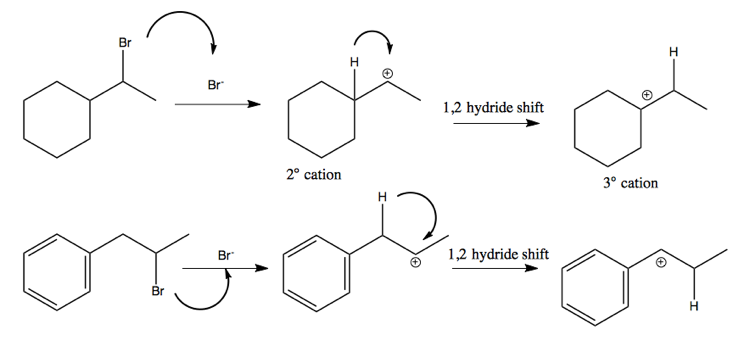
\includegraphics[width=0.7\textwidth]{1-2-hydride-shift-mechanism.png} \label{1-2-hydride-shift-mechanism}
\caption{Example of favorable hydride shift to generate tertiary carbocation from secondary carbocation intermediate.}
\end{figure}
\noindent Primary electrophiles proceed by \ce{S_N 2} while tertiary electrophiles proceed by \ce{S_N 1}. Secondary electrophiles can proceed by either \ce{S_N 1} or \ce{S_N 2}. Also, the stronger the nucleophile, the more likely the reaction will proceed by an \ce{S_N 2} mechanism; the better the leaving group, the more likely the reaction will proceed by an \ce{S_N 1} mechanism. Also, consider the following rate laws:
\begin{equation}
\begin{split}
\ce{S_N 1} \text{ Rate}=k\left[\text{Electrophile}\right]\\
\ce{S_N 2} \text{ Rate}=k\left[\text{Nucleophile}\right]\left[\text{Electrophile}\right]
\end{split}
\end{equation}
\noindent Lastly, you can also consider the solvent to distinguish between \ce{S_N 1} and \ce{S_N 2} reactions: if the solvent is protic (i.e. capable of forming hydrogen bonds), the reaction will have a tendency to proceed by an \ce{S_N 1} mechanism. If the solvent is aprotic (i.e. \textit{not} capable of forming hydrogen bonds), the reaction will have a tendency to proceed by an \ce{S_N 2} mechanism.

\subsection{Structure Elucidation}
When deducing the molecular structure for an organic molecule, it helps to know something about the symmetry of the compound and its units of unsaturation. The equation for units of saturation:
\begin{equation}
\begin{split}
\text{Units of Unsaturation} = \frac{2(\#C)+(\#N)-(\#H)-(\#X)+2}{2}
\end{split}
\end{equation}
\hilight{TODO} %TODO

\subsection{Lab Techniques}
Lab techniques can be broken down into three categories: separation, purification, and identification. \hilight{TODO} %TODO

\section{Physics}
\subsection{Translational Motion}
In general on the MCAT, although especially for the physics section, it's about speed more than precision. Important kinematic equations that you probably don't know yet:
\begin{equation}
\begin{split}
\Delta x = \frac{1}{2}\left(v_0+v_f\right)\Delta t, \quad v_f^2=v_0^2+2a\Delta x
\end{split}
\end{equation}

\subsection{Forces and Torque}
\indent In order to handle formula identification problems \textit{quickly} (as speed is extremely important on the exam), the two best techniques are \textbf{checking units} and considering \textbf{limiting cases}. For example, consider the following problem:
\begin{center}
\begin{minipage}{30em}
\textcolor{blue}{Example 2.3a\quad The pulley system shown below, sometimes referred to as an \textit{Atwood machine}, has two masses, $m_1$ and $m_2$. Which of the following formulas represents the acceleration of this system?
\begin{enumerate}[label=\Alph*]
	\item $a=\frac{\left(m_1-m_2\right)g}{m_1+m_2}$
	\item $a=\frac{\left(m_1+m_2\right)g}{m_1-m_2}$
	\item $a=\frac{g}{m_1+m_2}$
	\item $a=\frac{m_2g}{m_1+m_2}$
\end{enumerate}}
\end{minipage}
\end{center}
\noindent This problem essentially shows two masses, $m_1$, $m_2$, attached on two sides of the pulley. There's a traditional solution to \textit{actually} solve for the acceleration of the system, shown on pages 57-58 of TBR Physics, but this takes a lot of time. Instead, we can entirely avoid actually `solving' by using the fact that the test is multiple choice. Choices C and D don't have the right units, so they are definitely wrong. Distinguish between A and B by considering limiting cases. If $m_1=m_2$, then it should be zero acceleration, not infinite acceleration, so thus, the right answer is \textbf{A}. See how quickly we were able to arrive at the right answer?!\\
\indent Recall that torque $\mathbf{\tau}$ is defined to be $\mathbf{\tau}=\mathbf{r}\times\mathbf{F}$. The length is sometimes called the \textit{lever arm} or \textit{moment arm}, and the center of the bolt is called the \textit{pivot point}. \\
\indent Although it may sound strange and possibly incorrect when you first consider the idea, it is possible for a static friction to accelerate an object from rest. There are two \textit{everyday} examples that can help you to accept this concept: walking and driving. When you start walking from rest, you are clearly going from $v=0$ to having a velocity in the direction you are moving. This means that you have accelerated. This is achieved by \textit{pushing off} against the ground in a lateral direction. So, there must be a force accelerating you in a lateral direction. According to Newton's third law, there is an equal and opposite force as your push-off force. That opposing force is a static friction of the ground against your foot, as long as your foot does not slip. This explains why it is harder to start walking on an icy floor than a carpeted floow, because the static coefficient of friction $\mu_s$ for ice is much lower than $\mu_s$ for carpet. \\
\indent In physics and engineering, \textbf{mechanical advantage} is the factor by which a machine multiplies the force put into it. The mechanical advantage of a lever/see-saw can be described by the following equation:
\begin{equation}
\begin{split}
\text{mechanical advantage}=\frac{\text{weight of object}}{\text{applied force needed to support object}}=\frac{d_{\text{fulcrum}}}{d_{\text{weight}}}
\end{split}
\end{equation}
\noindent where $d_i$ is the distance from the fulcrum of object $i$. Example problems for force and torque:
\begin{center}
\begin{minipage}{30em}
\textcolor{blue}{9.\quad Which of the following graphs (see Figure \ref{Physics_1_2_9}) best represents the force due to static friction as incline angle increases for a redwood block atop a smooth rubber surface?}
\end{minipage}
\end{center}
\begin{figure}[h!]
\centering
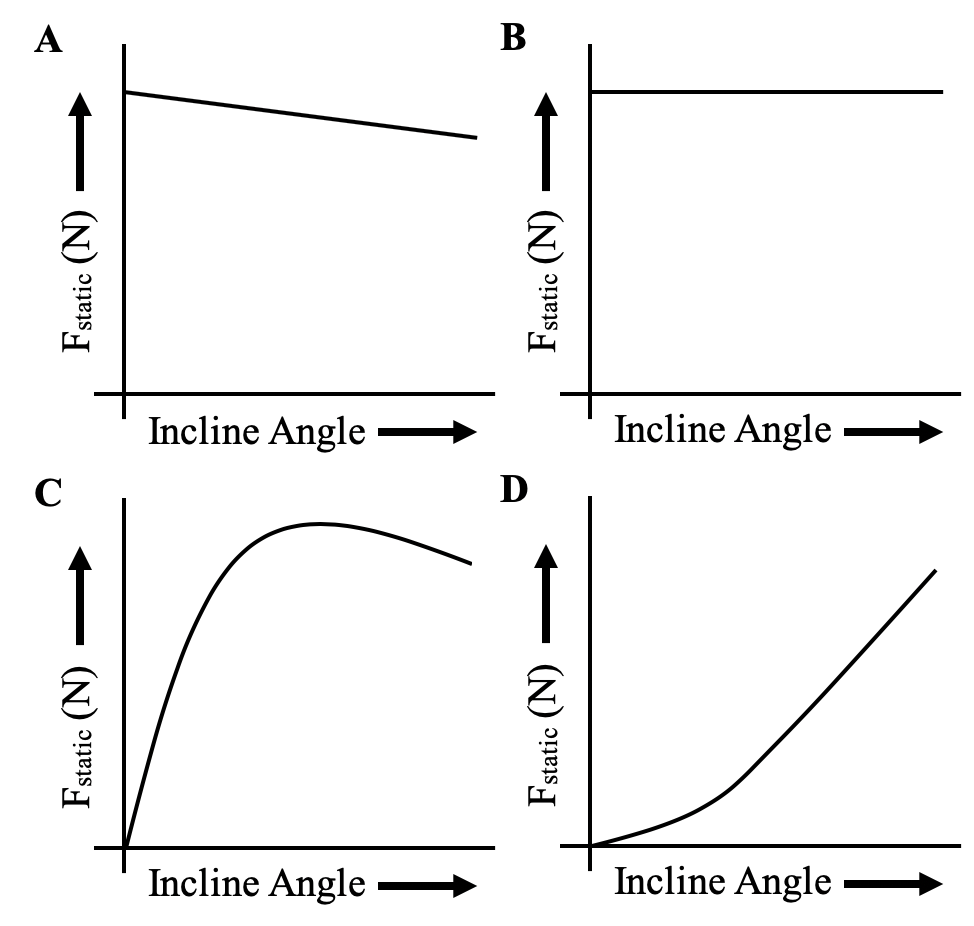
\includegraphics[width=0.4\textwidth]{Physics_1_2_9.png} \label{Physics_1_2_9}
\caption{Answer choices for Question 9 (Taken from Physics Part I, Passage II, Question 9 in TBR)}
\end{figure}
\indent Initially, you'd probably think that the answer is A; as you increase the incline angle, it makes sense the the static friction force would decrease, as this is what happens with the normal force, right? However, recall that static friction is a reactionary force, meaning that it is equal and opposite of any applied force. At zero inclination, the block has no inclination to move or anything like that, so the static friction is 0. As the block has more and more incentive to move as the incline angle increases (due to the force of gravity), the static friction must also increase in order to keep the block in place, until the object breaks free and begins to slide down the surface. Thus, the best answer choice in this instance is \textbf{D}. \\
\begin{center}
\begin{minipage}{30em}
\textcolor{blue}{22. If a person starts at the rim of a spinning platform and is pushed radially toward the central axis by a moving exterior wall, then what happens to the normal force felt by that person due to the wall?
\begin{enumerate}[label=\Alph*]
	\item It remains a constant.
	\item It decreases, since $r$ decreases.
	\item It increases, since $r$ decreases. 
	\item It decreases, since angular speed decreases.
\end{enumerate}}
\end{minipage}
\end{center}
\indent By Newton's third law, we know that the normal force felt by the person is equal to the force the person exerts on the wall, which is basically equal to the centripetal force $F_c=v^2/r$. Superficially, this looks like an inverse relationship $F_c\propto 1/r$, and so we may naively guess the answer is C. However, as $r$ decreases, $v$ also changes for circular motion! Rather, only angular frequency $\omega=v/r$ remains constant, so thus, the form of $F_c$ that we want to use is $F_c=\left(\omega r\right)^2/r=\omega^2r$. From this equation, it is clear that in reality, $F_c\propto r$, and so the correct answer is \textbf{B}.

\subsection{Work and Energy}
When negative work is done \textit{on} an object, it loses energy to its surroundings. Friction takes energy away from the sliding object. Generally, if \textit{positive} work is done \textit{on} the object, the object \textit{gains} energy. If \textit{the object does positive work}, the object \textit{loses} energy. If the work is negative, then the opposite would be true. For example, the work done on a block by friction as it slides on a rough surface is negative and directly proportional to $\mu_k$. The work done on a road surface, as a car skids across it, is positive and directly proportional to the skidding distance. \\
\indent The three forms of energy you need to know are kinetic energy, gravitational potential energy, and spring potential energy. Power is the rate of doing work/transferring energy with respect to time.\\
\indent Two simple machines that occasionally surface on the MCAT are the \textbf{inclined plane} and the \textbf{pulley system}. They make life easier, because they redirect and/or reduce the amount of \textit{force} we need to apply in accomplishing some task. However, they do not lessen the overall amount of work that must be done! It still requires the same amount of energy to carry out the task. This is to say that because energy is conserved, the amount of work needed to perform an action will be constant, no matter how the action occurs. Other simple machines include \textbf{levers} (as we saw in the rotational equilibrium section) and \textbf{hydraulic lifts} (which we will see in the fluids section).\\
\indent One way to characterize a machine is through its \textbf{mechanical advantage}, defined as
\begin{equation}
\begin{split}
\text{mechanical advantage}=\frac{\text{weight of the object to be supported}}{\text{applied force needed to support the object}}
\end{split}
\end{equation}
\noindent A machine with a bigger mechanical advantage will require less applied force than a machine with a smaller mechanical advantage when it is used to support some object. For pulleys in particular, note that the mechanical advantage is equal to the number of vertical cords supporting the moving pulley (page 111 in Physics Part I, TBR). \\
\indent Heat and work values are defined from the system's perspective in chemistry. When heat $q$ is positive, heat flows from the surroundings into the system. When $q$ is negative, heat flows from the system out to the surroundings. When work $w$ is positive, work is done on the system by the surroundings. When $w$ is negative, work is done by the system on the surroundings. \\
\indent The \textbf{Carnot cycle} converts either heat into work or work into heat. We inherently know the concept behind the Carnot cycle. When we blow on a hot liquid, it is done so with pursed lips. Consider blowing on the skin on the back of your hand. If you exhale through your moth with a normal, relaxed degree of aperture, your breath comes out at body temperature. But, if you exhale through your mouth with a small opening, the air feels cooler as it passes across your skin. That is due to the compression of the gas (exothermic) as it passes through your lips, and the expansion of the gas (endothermic) once it leaves your mouth. The air feels cooler, because it is expanding as it passes across the surface of your skin. When a gas expands, the molecules increase their intermolecular distance, which breaks intermolecular forces. Just as bond breaking is endothermic, so is the expansion of a gas. The process of blowing air on your skin through pursed lips results in heat transfer from a cold body (your skin) to a hot body (your mouth). This is unnatural heat flow, so it is similar to the function of the Carnot heat pump. Another example of a Carnot cycle is any piston engine.\\
\indent The \textit{refrigerator} uses work to absorb heat as a fluid passes through the four stages in a closed system. The basic idea is to put work energy into the system to compress a gas and condense it into a liquid. \\
\indent These are very complex topics. Just have the very fundamental perspective that a refrigerator takes in work (applied to a piston) and releases heat, while an engine takes in heat (to expand a gas in a piston) to release work. Do not overstudy this topic, even if you feel like you only partially comprehend it. \\
\indent Let's look at a couple of problems about work and energy:
\begin{center}
\begin{minipage}{30em}
\textcolor{blue}{9. Consider a pulley system with a flat metal lift plate (with negligible mass) attached to one side and a counterweight of 50 kg attached to the other side. A box with mass of 90 kg is placed on the metal plate. What is true of the total work associated with raising the box compared the work needed to raise the counterweight and return the left plate to the base position?
\begin{enumerate}[label=\Alph*]
	\item The work needed to raise the box exceeds the work needed to lift the counterweight.
	\item The work needed to raise the box is less than the work needed to lift the counterweight.
	\item The work needed to raise the box is equal to the work needed to lift the counterweight.
	\item No work is required to raise the box.
\end{enumerate}}
\end{minipage}
\end{center}
\indent Superficially, this seems like a very counterintuitive problem. Shouldn't it take no work at all to return the lift plate to the base? In actuality, the answer choices are simply talking about \textit{work}\textemdash this work doesn't need to be done by a person, as it can also be done by gravity. Thus, the work (done by us) needed to raise the box is 40 kg times $g$ (only 40 kg because of the counterweight), while the work (done by gravity) needed to restore the counterweight to its old position is 50 kg times $g$ (50 kg because that is the mass of the counterweight). Therefore, the correct answer is \textbf{B}.
\begin{center}
\begin{minipage}{30em}
\textcolor{blue}{18. After a hand pump has been operating, the shaft is warm and the tip of the needle is cool. This is because:
\begin{enumerate}[label=\Alph*]
	\item air is compressed in the shaft of the pump, and it expands as it enters the needle tip.
	\item air is compressed in the shaft of the pump, and it expands as it leaves the needle tip.
	\item air expands in the shaft of the pump, and it is compressed as it enters the needle tip.
	\item air expands in the shaft of the pump, and it is compressed as it leaves the needle tip.
\end{enumerate}}
\end{minipage}
\end{center}
\noindent We are given that the shaft is warm and the tip is cool. This means that the air is compressed in the shaft (because compressing the air is an exothermic processes where heat is released into the shaft) and expanded in the tip (because the gas molecules have more kinetic energy and absorb this energy from the environment, thus cooling the needle tip). This eliminates answer choices C and D. Just as we blow air out of our mouth, the air should be leaving the needle tip, not entering it, so thus, the correct answer choice is B. 

\subsection{Periodic Motion}
The \textbf{crest} is the maximum of a wave and the \textbf{trough} is the minimum of a wave. Frequency and period for a cyclic process are inverses of one another and are related by the equation $f=1/T$. If a system loses energy as it goes, we refer to this as \textit{dampened harmonic oscillation}. The dampening is often caused by friction as the mass slides across the surface. The two most important periodic motion set ups that you should know are the pendulum and spring:
\begin{equation}
\begin{split}
F_{\text{pendulum}}=-mg\sin\theta, \quad U_{\text{pendulum}}=-mgL\left(1-\cos\theta\right), \quad T_{\text{pendulum}}=2\pi\sqrt{\frac{L}{g}}, \quad f_{\text{pendulum}}=\frac{1}{2\pi}\sqrt{\frac{g}{L}}\\
F_{\text{spring}}=-kx, \quad U_{\text{spring}}=\frac{1}{2}kx^2, \quad T_{\text{spring}}=2\pi\sqrt{\frac{m}{k}}, \quad f_{\text{spring}}=\frac{1}{2\pi}\sqrt{\frac{k}{m}}
\end{split}
\end{equation}
\noindent Transverse waves cause vibrations perpendicular to the direction of wave propagation (i.e. the `wave' at sports events), while longitudinal waves cause vibrations parallel to the direction of wave propagation (i.e. sound waves). The speed $v$ of a wave is $v=\lambda f$. In the particular case of a transverse wave propagating along a string, the speed $v=\sqrt{T/\mu}$, where $T$ is the tension in the string and $\mu$ is the mass per unit length. \\
\indent A phenomenon known as a \textbf{beat} occurs when two waves of differing wavelengths wavelengths interfere with each other. Generally, if waves of frequency $f_1, f_2$ interfere, they will give rise to a beat frequency of $f_{\text{beat}}=|f_2-f_1|$. \textbf{Standing waves} are disturbances/waves that do not appear to travel along their line of propagation. Areas of no vibration are referred to as \textbf{nodes}. The area of the vibration where the amplitude is the largest is referred to as an \textbf{antinodes}. For the purposes of the MCAT, antinodes are found symmetrically displaced between adjacent nodes. The allowed standing-wave harmonic frequencies are given by $f_n=\frac{nv}{2L}$, where $n$ is a natural number and $v$ is the velocity of the wave. The allowed standing-wave frequencies are given by $\lambda_n=\frac{2L}{n}$. \\
\indent The amplitude, and hence the energy of the system, may increase if we supply a vibrating force that has a frequency which is the same as the natural frequency of the system. This phenomenon is called \textbf{resonance}. The key to identifying resonance phenomena is to recognize that a given passage involves some object that can vibrate, an applied vibrational force, and a match between the natural and forced vibration frequencies. \\
\indent Note that in basically all of the cases we are considering in the MCAT, fixed-end vibrating strings in a harmonic oscillation have the same wave speed at any point on the string. 

\subsection{Fluids and Fluid Statics}
By definition, a \textit{fluid} is any matter that flows. The \textbf{specific gravity} (also called the \textbf{relative density}) of a material is defined as the ratio of its density to the density of water at $4^{\circ}$C. That is,
\begin{equation}
\begin{split}
\text{Specific gravity}=\rho_{\text{relative}}=\frac{\rho_{\text{material}}}{\rho_{\ce{H_2O}\text{ at }4^{\circ}\text{C}}}
\end{split}
\end{equation}
\noindent \textit{Pascal's Principle} states that a pressure applied to an enclosed fluid is transmitted equally throughout the fluid and to the walls of the fluid's container. Mathematically, consider a column of liquid with pressure $p_1$ at height $y_1$ and pressure $p_2$ at height $y_2$, with $y_1<y_2$ and $p_1>p_2$ since $y_1$ is lower than $y_2$ on the $y$-axis (which points upwards). Then, Pascal's principle states that
\begin{equation}
\begin{split}
p_1-p_2=\rho\left(y_2-y_1\right)g
\end{split}
\end{equation}
\noindent Let's consider an example problem:
\begin{center}
\begin{minipage}{30em}
\textcolor{blue}{At a specific depth in a swimming pool, a barometer measures the total pressure to be twice that of atmospheric pressure. If the barometer is now submerged to a depth that is twice its initial depth, by how much does the total pressure increase?
\begin{enumerate}[label=\Alph*]
	\item The pressure increases by $50\%$.
	\item The pressure increases by $100\%$.
	\item The pressure increases by $200\%$.
	\item The pressure increases by $300\%$.
\end{enumerate}}
\end{minipage}
\end{center}
\noindent To solve this problem, we can use the \textit{ratio technique}. We have that, since pressure is additive,
\begin{equation}
\begin{split}
p_{\text{total}}=p_{\text{atm}}+\rho gh
\end{split}
\end{equation}
\noindent From the given information, we know that $\rho gh_{\text{initial}}=p_{\text{atm}}$, since the total pressure there is $2p_{\text{atm}}$. If the second depth is twice that of the first, then $\rho gh_{\text{final}}=2p{\text{atm}}$, meaning that the total pressure at the second depth is $3p_{\text{atm}}$. Taking the ratio fo the final to the initial situation gives
\begin{equation}
\begin{split}
\frac{p_{\text{total final}}}{p_{\text{total initial}}}=\frac{3p_{\text{atm}}}{2p_{\text{atm}}}=1.5
\end{split}
\end{equation}
\noindent To complete this problem, just subtract $1$ from the ratio to get the percentage change of $+0.5$ (i.e. $50\%$). Be careful of the wording in percentage questions. Here, we want a `percentage \textbf{change}'. If the question had asked instead, `What percentage of the initial total pressure \textbf{is} the final total pressure?', the answer would have been `The final total pressure is $150\%$ of the initial total pressure.' Long story short, the best answer is choice \textbf{A}. \\
\indent \textbf{Archimedes' Principle} states that the buoyant force $B$ experienced by an object is
\begin{equation}
\begin{split}
B=\rho_{\text{fluid}}\cdot V_{\text{fluid displaced}}\cdot g
\end{split}
\end{equation}
\indent The following figure shows a summary of the mathematics associated with a floating object and a sunken object in a tank of fluid:
\begin{figure}[h!]
\centering
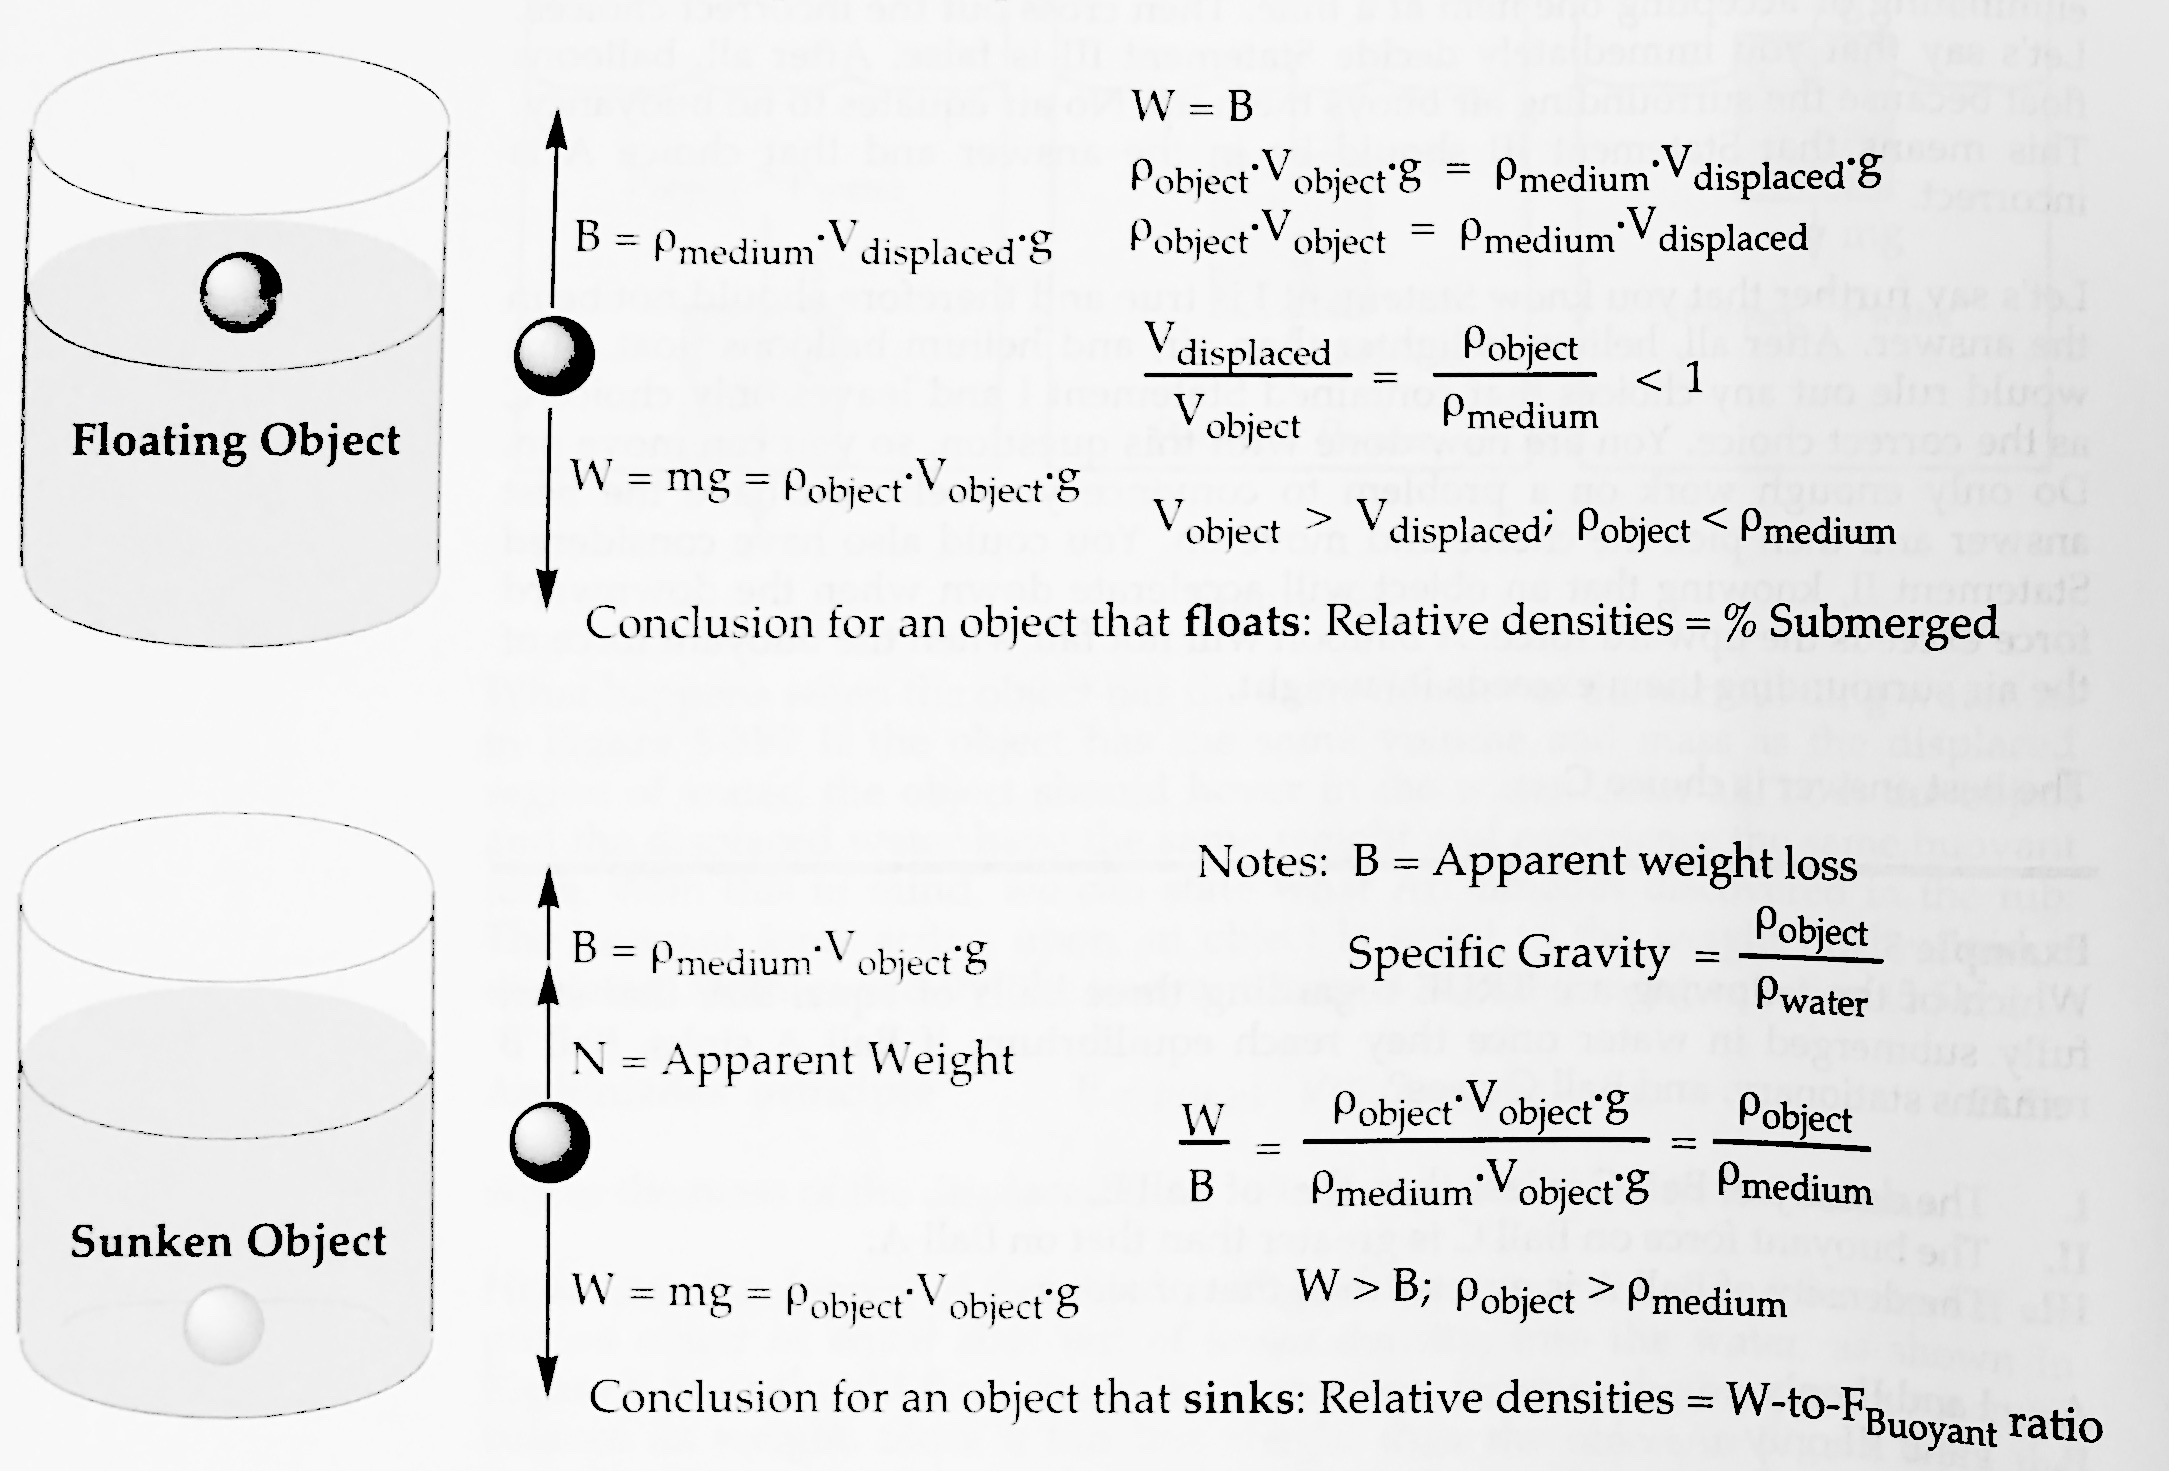
\includegraphics[width=0.8\textwidth]{IMG_3047} \label{3047}
\caption{Mathematics of Objects placed in Tanks of Fluid}
\end{figure}
\noindent Here is an example problem associated with the information shown in \textbf{Figure \ref{3047}}:
\begin{center}
\begin{minipage}{30em}
\textcolor{blue}{What is the specific gravity of an object that weighs 36N in air but only 9N in water at $4^{\circ}$C?
\begin{enumerate}[label=\Alph*]
	\item 0.25
	\item 1.33
	\item 3.00
	\item 4.00
\end{enumerate}}
\end{minipage}
\end{center}
\noindent Because the object still has weight in water, this means that the object is a sunken object rather than a floating object. Thus, the object must be denser than the medium, so the specific gravity must be greater than 1. Based on the given information, the buoyant force must be 27N. Keep in mind that a sunken object rests on the bottom of the container, where because it experiences no acceleration, it has a net force of zero. This means that on the bottom fo the tank, $mg=N+B$, where $N$ is the perceived weight of the object in water, $B$ is the buoyant force, and $mg$ is the actual weight of the object in water. To get the specific gravity (the relative densities), we simply divide 36 by 27:
\begin{equation}
\begin{split}
\text{Specific Gravity}=\frac{W}{B}=\frac{36\text{N}}{27\text{N}}=\frac{4}{3}=1.33
\end{split}
\end{equation}
\noindent Thus, the correct answer is \textbf{B}. \\
\indent The force associated with the tendency of the surface of a liquid to pull inward and shrink in area is known as \textbf{surface tension}. This is largely due to intermolecular forces such as hydrogen bonding or van der Waals interactions. 

\subsection{Viscosity and Poiseuille's Principle}
Friction in fluids is called \textbf{viscosity} ($\eta$), which units of $\text{N}\cdot\text{sec}/\text{m}^2$. Viscous forces retard the motion of one part of a fluid relative to another part of the fluid. If two layers of a fluid are held together tightly, then the viscosity of the fluid is said to be large, and the fluid will move \textit{slowly}. Generally, when the temperature of a fluid \textit{increases}, the viscosity of a liquid would \textbf{decrease} while the viscosity of a gas would \textbf{increase}. When a simple fluid flows through a pipe, the speed of that fluid is greatest at the central axis of the pipe and essentially zero along the walls of the pipe. As a fluid is flowing through the \textbf{center} of a pipe of length $L$ with a certain speed $v$, there is a force that tends to oppose the fluid's motion. That force is called a \textbf{\textit{viscous retarding force}} $F$ and it is caused by the fluid's resistance to flow. The magnitude of $F$ is given by
\begin{equation}
\begin{split}
F=4\pi\eta L v
\end{split}
\end{equation}
\noindent The net force on a fluid is proportional to the difference between the pressures of the pipe at the different ends. For the fluid to flow through the center of the pipe at constant speed, the driving force and the retarding force must be equal. If we substitute the cross sectional area $A=\pi r^2$ for a pipe, then we get
\begin{equation}
\begin{split}
4\pi\eta Lv=A\left(p_1-p_2\right)\longrightarrow v=\left(\frac{p_1-p_2}{4\eta L}\right)r^2
\end{split}
\end{equation}
\indent The \textbf{volume flow rate} $Q$ is the volume $V$ of fluid that passes through a pipe per unit time. Recall that we have mentioned that the fluid in a pipe flows the fastest at the center of the pipe and does not flow at all at the edges of the pip. Using this assumption, we can express the average speed of the fluid as $\bar{v}=v/2$. If we also assume a circular cross-sectional area of $A=\pi r^2$, then we can arrive at $Q=V/t=\left(v/2\right)\pi r^2$. Plugging in the result from earlier for the speed of fluid flow, we arrive at \textbf{Poiseuille's Principle}:
\begin{equation}
\begin{split}
Q=\frac{\pi r^4}{8\eta L}\left(p_1-p_2\right)
\end{split}
\end{equation}
An important parameter in Poiseuille's Principle is the $r^4$ term. Note that if the radius of the pipe is doubled, the flow rate increases by a factor of 16. Although we have presented Poiseuille's Principle as a mathematical expression to this point, at the level of the MCAT it is highly conceptual. For instance, it explains that an extremely tall person will have a greater strain on their hair than a person of average height, because in order to generate the same volume flow rate $Q$, a tall person requires a greater $\Delta p$ to offset the greater $L$ associated with their longer circulatory system.

\subsection{Continuity Equation}
Assuming that fluid is incompressible, at any given moment in time, the fluid entering one region with cross sectional area $A_1$ must equal the fluid leaving the region at $A_2$. In other words, the volume flow rates for the two regions must be equal. This gives us the \textbf{continuity equation}
\begin{equation}
\begin{split}
Q=A_1\bar{v}_1=A_2\bar{v}_2
\end{split}
\end{equation}
\noindent The continuity equation can also apply to branching as long as the fluid is incompressible and that the total cross-sectional areas of all the branches is considered. Here is an example of a problem involving the continuity equation:
\begin{center}
\begin{minipage}{30em}
\textcolor{blue}{Atherosclerosis is the thickening and hardening of the arterial walls. The aorta of a healthy adult has a radius of about 1.3 cm and a blood flow velocity of about 0.5 m/s. An atherosclerosis-stricken bacon epicure is found to have an effective aortic radius that is 75\% of that in a healthy aorta. What is the blood flow velocity through the narrowed section of the artery? (Assume that the blood's volumetric flow rate is constant for all adults.)
\begin{enumerate}[label=\Alph*]
	\item 0.28 m/s
	\item 0.38 m/s
	\item 0.66 m/s
	\item 0.89 m/s
\end{enumerate}}
\end{minipage}
\end{center}
\noindent This problem is easily solved using the continuity equation:
\begin{equation}
\begin{split}
A_1\bar{v}_1=A_2\bar{v}_2\rightarrow\bar{v}_2=\frac{A_1}{A_2}\bar{v}_1=\frac{\pi \left(1.3\text{ cm}\right)^2}{\pi \left(0.75 \cdot 1.3\text{ cm}\right)^2} \left(0.5\text{ m/s}\right)=\frac{16}{9}\frac{1}{2}\text{ m/s}=\frac{8}{9}\text{ m/s}\approx 0.89 \text{ m/s}
\end{split}
\end{equation}
\noindent Therefore, the best answer choice is \textbf{D}. 

\subsection{Bernoulli's Equation}
Bernoulli's Equation stems from the work-energy theorem as applied to a moving fluid system. \hilight{TODO} %TODO

\subsection{Turbulence}
When we looked at Poiseuille's Principle, we say that adjacent layers of a fluid have the ability to slide past one another in a smooth and uniform fashion. This is called \textbf{laminar} flow. Poiseuille's Principle only holds for laminar flow. If the flow of a fluid is sufficiently high, then a chaotic and irregular pattern develops in the fluid\textemdash this is called \textbf{turbulent} flow. Viscous frictional forces increase during turbulent flow.\\
\indent The \textbf{Reynolds number} $N_R$, defined by
\begin{equation}
\begin{split}
N_R=\frac{2\rho\bar{v} R}{\eta}
\end{split}
\end{equation}
\noindent tells us whether flow is laminar or turbulent, where $\rho$ is the density of the fluid, $\eta$ is the viscosity, $\bar{v}$ is the average velocity of the fluid, and $T$ is the radius of the vessel through which the fluid flows. $N_R<2000$ means the flow is laminar, $N_R>3000$ means the flow is turbulent, and anywhere in between means the flow is unstable. This means that flow can be either laminar or turbulent depending on the material. Here's an example of a problem involving turbulence:
\begin{center}
\begin{minipage}{30em}
\textcolor{blue}{Which of the following will decrease the chance of turbulent blood flow in a vein?
\begin{enumerate}[label=\Alph*]
	\item Widening the vein while maintaining the same flow speed.
	\item Thinning the blood without changing its density.
	\item Increasing the absolute pressure on each end of the vein by the same amount.
	\item Lowering the blood density without thinning it.
\end{enumerate}}
\end{minipage}
\end{center}
\noindent Widening the vein increases $R$, which increases the Reynold's number and thus the chance of turbulent flow, so choice A is eliminated. Thinning the blood decreases $\eta$, which increases the Reynold's number and thus the chance of turbulent flow, so choice B is eliminated. Increasing the absolute pressure on each end of the vein doesn't do anything according to the mathematical definition of the Reynold's number, so choice C is eliminated. Lowering the blood density decreases $\rho$, which decreases the Reynold's number and thus the chance of turbulent flow, so choice \textbf{D} is the correct answer.

\subsection{Electrostatics}
The mass of a proton is about 1800 times greater than the mass of an electron, and the mass of a neutron is approximately equal to the sum of a proton and electron. Coulomb's Law is given by
\begin{equation}
\begin{split}
F_e=k\frac{q_1q_2}{r^2}
\end{split}
\end{equation}
\noindent Field lines always originate on a positive charge and end of a negative charge. They represent the way a (+) charge would migrate. Equipotential lines and electric field lines are \textit{perpendicular} to one another. The electrical potential energy of particles with like charges increases when the charges are brought towards each other. Conversely, the electrical potential energy decreases when opposite charges are brought towards each other. Opposite charges naturally attract; as they approach one another, their potential energy decreases. The reverse applies when two like charges are brought towards each other:
\begin{equation}
\begin{split}
\Delta PE_q = kq_1q_2\left(\frac{1}{r_f}-\frac{1}{r_i}\right)=qV
\end{split}
\end{equation}
\noindent The $qV$ part applies when we want to calculate the change in electrical potential energy as a charged particle is moving through a voltage difference.\\
\indent The \textbf{dielectric constant} $\kappa$ is the ratio of the electrical force between two charges when they are in a vactuum compared to when they are in a medium. Mathematically,
\begin{equation}
\begin{split}
F_{\text{medium}}=\frac{F_{\text{vacuum}}}{\kappa}
\end{split}
\end{equation}
\noindent A strongly polar medium responds to an external electric field by reorienting its polar molecules, so that the net electric field within the medium becomes weaker than the external field.This occurs when the partial positive charges of the medium align near the negative plate and the partial negative charges align near the positive plate. Such a field strength reduction diminishes the interactive forces between all charges within the medium. Coulomb's law can be modified for dielectrics:
\begin{equation}
\begin{split}
F_{\text{medium}}=\frac{F_{\text{vacuum}}}{\kappa}=\frac{k\left|q_1q_2\right|}{\kappa r^2}
\end{split}
\end{equation}
\noindent Note that when solid materials melt, their polarizability normally increases, meaning their dielectric constant increases. However, as temperature continues to increase, thermal motion subsequently reduces its polarizability because the high kinetic energy eventually surpasses the electrostatic interactions that led to the polarizability.\\
\indent An \textbf{electric dipole} is established when two charges of opposite signs are separated from one another by some distance $L$. If $p$ is defined to be the \textbf{dipole moment}, $q$ is the charge, and $L$ is the distance separating the charges $+q$ and $-q$, then we have 
\begin{equation}
\begin{split}
\mathbf{p}=q\mathbf{L}
\end{split}
\end{equation}
\noindent by definition. The net force on an electric dipole in a uniform external electric field is zero. However, dipoles can experience a net torque. If we let the angle between the dipole axis and electric field be $\theta$, then the torque created by the dipole couple can be quantified by
\begin{equation}
\begin{split}
\mathbf{\tau}=\mathbf{E}\times\mathbf{p}=qEL\sin\theta=pE\sin\theta
\end{split}
\end{equation}
\noindent The torque is at its minimum when $\mathbf{p}$ and $\mathbf{E}$ are parallel (or antiparallel) to one another, and at its maximum when $\mathbf{p}$ and $\mathbf{E}$ are perpendicular to one another. The potential energy $PE$ of the system can be given by
\begin{equation}
\begin{split}
PE=-pE\cos\theta
\end{split}
\end{equation}
\noindent Notice that the potential energy of the system is lowest (i.e. the system is most stable) when the dipole is parallel to the electric field, and highest (i.e. the system is least stable) when the dipole is antiparallel to the electric field. 

\subsection{Electromagnetism}
Magnetic fields can exert a magnetic force $F_{\text{magnetic}}$ on a charge moving in that field, known as the Lorentz force:
\begin{equation}
\begin{split}
\mathbf{F_{\text{magnetic}}}=q\mathbf{v}\times\mathbf{B}=qvB\sin\theta
\end{split}
\end{equation}
\noindent where $\theta$ is the angle between the velocity $\mathbf{v}$ of the particle and the external magnetic field $B$. \\
\indent A \textbf{solenoid} is a helical winding of a conducting wire, such as a coil of copper wire would on a cylindrical tube. The strength of the magnetic field $B$ inside the solenoid is $B=\mu_0nI$, where $I$ is the current and $n$ is the number of turns per unit length in the solenoid.\\
\indent The combination of electric and magnetic forces can often be used to select for particles with certain velocities. Imagine a long chamber with an electric field $F_e=qE$ pointing down and a magnetic field $F_b=qvB$ pointing up (with the magnetic field pointing into the page). If we shoot particles with a distribution of velocities into the chamber, then particles that are too fast have $F_b>F_e$, meaning they deflect up, while particles that are too slow have $F_e<F_b$, meaning they deflect down. If $v=E/B$, when the particle travels straight and makes it through the chamber.

\subsection{Electricity and Electric Currents}
By definition, current flows in the same direction in which positive charges flow and in the direction opposite to that in which negative charges flow. Thus, current flows from regions of higher electrical potential to regions of lower electrical potential. \\
\indent A \textbf{galvanic cell} converts chemical potential energy into an electromotive force (emf) that generates electrical flow. The \textbf{anode} is the source of electrons and is the negatively charged pole, while the \textbf{cathode} is the endpoint of electron flow and is the positively charged pole. The \textbf{resistivity} $\rho$ of a material is a measure of how difficult it is for charges to conduct through the material; higher resistivities are associated with better electrically insulating materials. The resistivity relates to the current density $J$ and the electric field $E$, as $\rho=E/J$. \textbf{Conductivity} $\sigma=1/\rho$ is the reciprocal of resistivity. The larger the conductivity of a material, the better that material is at conducting current, so a material with low resistivity has high conductivity. The \textbf{resistance} $R$ of a conductor is $R=\rho L/A$, where $L$ is the length of the resistor and $A$ is the cross sectional area of the resistor. In general, resistors oppose the flow of current, and thus drain energy/power from electrical circuits. \textbf{Power} $P$ is the rate of conversion of electrical potential energy into some other type of energy:
\begin{equation}
\begin{split}
P=IV=\frac{V^2}{R}=I^2R
\end{split}
\end{equation}
\noindent A \textbf{capacitor} is formed from two conductors separated by an insulator. The \textbf{capacitance} $C$ of a capacitor is $C=q/V$; in other words, it is the amount of charge $q$ that can be stored per volt of potential difference $V$ across the two parallel plates. For the parallel plate capacitor, we usually have
\begin{equation}
\begin{split}
C=\frac{\kappa}{4\pi k}\frac{A}{d}
\end{split}
\end{equation}
\noindent where $\kappa$ is the dielectric constant, $A$ is the area of the plate, and $d$ is the distance between the capacitor plates. \\
\indent The MCAT only tests RC circuits that feature resistor(s) and capacitor(s) in series. \textbf{Kirchhoff's loop rule} states that the algebraic sum of the potential differences in any closed circuit loop is zero. \textbf{Kirchhoff's junction rule} states that the total current flowing through the pathways leaving the junction must equal the current that entered the junction. Resistors add in series and capacitors add in parallel. Consider the following two practice problems: 
\begin{center}
\begin{minipage}{30em}
\textcolor{blue}{What is true of the voltage across, charge stored on, and energy stored by two unequal capacitors connected in parallel?
\begin{enumerate}[label=\Alph*]
	\item The larger capacitor has a smaller voltage gain and stores less energy; both capacitors store the same charge.
	\item The larger capacitor stores more charge and more energy; both capacitors have the same voltage gain.
	\item The larger capacitor stores more charge and has a smaller voltage gain; both capacitors store the same energy.
	\item The larger capacitor stores less charge and has a larger voltage gain; both capacitors store the same energy.
\end{enumerate}}
\end{minipage}
\end{center}
\noindent When charge stores in a parallel capacitor circuit, the voltage drop across each capacitor is the same. Given that the voltage is the same, the larger capacitor will store more charge, since $Q=CV$. The larger capacitor will also store more energy, since $\Delta PE_q=\frac{1}{2}CV^2$. Therefore, the correct answer is \textbf{B}. 
\begin{center}
\begin{minipage}{30em}
\textcolor{blue}{What is true of the voltage across, charge stored on, and energy stored by two unequal capacitors connected in series?
\begin{enumerate}[label=\Alph*]
	\item The larger capacitor has a smaller voltage gain and stores less energy; both capacitors store the same charge.
	\item The larger capacitor stores more charge and more energy; both capacitors have the same voltage gain.
	\item The larger capacitor stores more charge and has a smaller voltage gain; both capacitors store the same energy.
	\item The larger capacitor stores less charge and has a larger voltage gain; both capacitors store the same energy.
\end{enumerate}}
\end{minipage}
\end{center}
\noindent When charge stores in a series capacitor circuit, the charge stored on each capacitor will be the same. Since the voltage drop across each capacitor is $V=Q/C$, this means that the larger capacitor will have a smaller voltage gain. The larger capacitor also stores less energy, since $\Delta PE_q=\frac{1}{2}\frac{Q^2}{C}$. Therefore, the correct answer is \textbf{A}. \\
\indent To summarize, let's rehash the differences between parallel circuit elements and series circuit elements:
\begin{table}[!ht]
\begin{tabular}{ll}
\textbf{Series Circuit Elements} & \textbf{Parallel Circuit Elements} \\
\text{Same current} & \text{Different current} \\
\text{Different voltage drop} & \text{Same voltage drop} \\
\text{Increased equivalent resistance} & \text{Reduced equivalent resistance} \\
\text{Reduced equivalent capacitance} & \text{Increased equivalent capacitance} \\
\text{Larger resistors drain more power} & \text{Smaller resistors drain more power} \\
$P=I^2R$ & $P=V^2/R$ \\
\text{Devices are dependent of one another} & \text{Devices are independent of one another}
\end{tabular}
\end{table}
\noindent Lastly, if we consider all the electrons of a conducting metal, and thus all of the electron levels shared between the metal atoms, we get what is known as \textit{band theory}\textemdash electrons fill from the bottom levels up, so only a few electrons are actually in high enough energy levels to be able to transfer. The level up to which the electrons fill is called the \textit{Fermi level}. For metals with low enough ionization energy, the electrons in and near the Fermi level are free to flow.

\subsection{Light and Radiation}
Light in the 400 nm to 700 nm range can be detected by the retina and processed in the brain, leading to the phenomenon of color. Remember that in the presence of an external light source, an object will appear a certain color but then absorb the complementary color (which is why it appears as the particular color). The \textbf{photoelectric effect} basically says that an incident photon can cause the release of an electron, so long as the photon has an energy greater than the ionization limit of the material. The energy required to remove an electron from the surface of the solid material is referred to as the \textit{work function}, $\phi$. Energy in excess of the work function becomes kinetic energy for the electron that is emitted. Mathematically, the photoelectric effect is represented as
\begin{equation}
\begin{split}
h\nu=\phi+\frac{1}{2}mv^2
\end{split}
\end{equation}
\noindent The \textbf{threshold frequency} corresponds to the photon equal in energy to the work function. Any photon with a frequency less than the threshold frequency does not have enough energy to ionize the material. \\
\indent If unpolarized light is passed through a perfect polarizing filter, the vectors would radiate in only one plane, as the light wave has been linearly polarized. The polarizing filter blocks all light perpendicular to the polarizing axis, but it allows the light aligned with the polarizing axis to pass through. \\
\indent When talking about interference, an important thing to bring up is Young's double-slit experiment. If two slits are separated by a distance $d$, and are a distance $L$ away from some screen with $L\gg d$, and light with a wavelength of $\lambda$ is sent through both slits, then the distance $y$ between two adjacent maxima of the interference pattern is 
\begin{equation}
\begin{split}
y=\frac{\lambda L}{d}
\end{split}
\end{equation}
\noindent Here is an example problem involving interference patterns:
\begin{center}
\begin{minipage}{30em}
\textcolor{blue}{When laser light is sent through two slits, a periodic pattern of constructive and destructive spots appears on a distant viewing screen. Suppose the two slits are now replaced with a \textbf{diffraction grating} (essentially several slits, which can be assumed to be infinitesimally small). If the same total light intensity is used in both the double-slit and the diffraction grating experiments, then the bright spots of the interference pattern in the diffraction grating will be:
\begin{enumerate}[label=\Alph*]
	\item more intense and spaced together more closely than in the double-slit experiment.
	\item more intense and spaced farther apart than in the double-slit experiment.
	\item less intense and spaced together more closely than in the double-slit experiment.
	\item less intense and spaced farther apart than in the double-slit experiment.
\end{enumerate}}
\end{minipage}
\end{center}
\noindent Without going into depth, we know that a fixed amount of light should reach the screen, so if the number of spots decreases, the intensity of each remaining spot should increase. This makes choices C and D highly unlikely answers. Similar to Young's double slit experiment with two slits, in the diffraction grating, the constructive spots will appear when the light rays from all slits are interfering as constructively as they can. Since the light rays emanating from several slits must now interfere in phase, the likelihood of a maximum is much small than it is in the double-slit experiment. The diffraction grating maxima will also be much narrower than the double-slit maxima. Thus, the maxima intensity must be greater for the diffraction grating experiment. Thus, the best answer is choice \textbf{B}. Here is another example problem:
\begin{center}
\begin{minipage}{30em}
\textcolor{blue}{A thin layer of plastic ($n=1.46$) coats the surface of a glass plate ($n=1.52$). When monochromatic light is shined normally onto the plastic from the air above, constructive interference occurs. Destructive interference will occur when the coated glass is immersed in which of the following liquids?
\begin{equation}
\begin{split}
\textbf{I. }&\text{ Water} \left(n=1.33\right)\\
\textbf{II. }&\text{ Carbon Tetrachloride} \left(n=1.46\right)\\
\textbf{III. }&\text{ Benzene} \left(n=1.50\right)
\end{split}
\end{equation}
\begin{enumerate}[label=\Alph*]
	\item I only
	\item I and III only
	\item II and III only
	\item III only 
\end{enumerate}}
\end{minipage}
\end{center}
\noindent The system involves light traveling from air ($n=1$) to plastic ($n=1.46$) to glass ($n=1.52$). Phase flips of light occur when the light bounces off a medium whose refractive index \textit{exceeds} that of the medium through which the light passes. In the original constructive set-up, light bounces off of an air-plastic interface and a plastic-glass interface. For both reflections, the refractive index of the reflecting medium is greater than that of the medium through which the light passes. For both reflections, the phase of the light will flip by $180^{\circ}$. To get destructive interference, we would need to change the experiment such that one of these two phas flips does not occur. If this is achieved, the single-phase flip would lead to destructive (i.e. $180^{\circ}$ out-of-phase) interference between the two final rays. This happens only with benzene, so the correct answer choice is choice \textbf{D}. \\
\indent This problem demonstrates the following: when a wave reflects from an optically denser medium, its phase flips $180^{\circ}$. Consider a film of oil on water, in air. The phase flips for both the wave that reflects off of the air-oil interface and the wave that reflects off of the oil-water interface. In both cases, the light bounces off a material whose refractive index $n$ is higher than that of the material through which the wave moves. Thus, the phases of both waves flip, the effect cancels, and the waves interfere constructively. Now, if the oil film was replaced with a soap film, then only one of the two reflecting waves flips its phase. This single flip effectively adds half a wavelength to the path-length difference and results in destructive interference.\\
\indent \textbf{Diffraction} is the distortion/bending of light waves when they pass through an opening or around an object. It is more significant when the wavelength is larger than or comparable to the opening the wave crosses. Diffraction is less significant or negligible when the wavelength is much smaller than the opening. This applies to all waves. 

\section{Biochemistry and Molecular Cell Biology}
\subsection{Amino Acids and Proteins}
All of the standard 20 amino acids are referred to as \textit{$\alpha$-amino acids} (i.e. a 2-amino acid), except for \textit{proline} which is referred to as an \textit{$\alpha$-imino acid}. Configurations (either relative or absolute) in amino acids refers to the stereochemical configuration around the chiral carbon. Due to differences in the priority of different amino acid side chains, not all amino acids have the same ``absolute configuration,'' which refers the R/S naming convention. However, all amino acids have the same ``relative configuration,'' which refers to the D/L naming convention. All biologically produced amino acids are in the L configuration. \\ 
\indent The charged R groups are Asp (aspartate), Glu (glutamate), Lys (lysine), Arg (arginine), and His (histidine). All of these are highly ionized at neutral pH except for His, which is only weakly ionized.\\
\indent Body fluids have pH range from 6.5 to 8.0\textemdash at these ranges, the amino and carboxyl groups are ionized. In other words, the $\alpha$-amino group bears a positive charge, while the $\alpha$-carboxyl group bears a negative charge. This is referred to as the \textbf{zwitterionic} nature of amino acids, due to the fact that the pKa of the $\alpha$-amino terminal is about 9.4, while it is about 2.2 for the $\alpha$-carbxyl terminal. Since amino acids can act as either an acid or a base, they are referred to as \textbf{ampholytes}. To determine the fraction of either the $\alpha$-amino, $\alpha$-carboxyl, or side chain groups that are ionized at a particular pH, use the \textbf{Henderson-Hasselbalch Equation}:
\begin{equation}
\begin{split}
\ce{pH}=\ce{pK_a}+\log\frac{\ce{[A^-]}}{\ce{[HA]}}
\end{split}
\end{equation}
\noindent The \textbf{isoelectric point} is the pH at which an amino acid carries \textbf{no net} electric charge. From the Henderson-Hasselbalch Equation, we know that the isoelectric point pI can be rewritten as
\begin{equation}
\begin{split}
\ce{pI}=\frac{\ce{pK_{a1}+pK_{a2}}}{2}
\end{split}
\end{equation}
\noindent Basically, it's just the main of all of the pKa values associated with the side groups for the molecule. For most amino acids, you only need to factor in the $\alpha$-COOH and $\alpha$-N$\text{H}_3^+$ pKa values, although the R side group may also contribute as well. In terms of making buffers, if a weak acid is within 1 pH unit of its pKa value, it resides within a good buffering range.\\
\indent Polypeptides with a net positive charge at physiologic pH (\textasciitilde7.4) most likely contain amino acids with \textit{basic} R groups. Polypeptides with a net negative charge at physiologic pH most likely contain amino acids with \textit{acidic} R groups. \\
\indent Electrophoretic separation of leucine from a protein sample would be least effective at pH 7.4, as opposed to pH values of 2.4, 1.4, and 0.4, because leucine has an aliphatic side chain, and so at physiological pH, leucine exists as a zwitterion. \\
\indent Formation of \textbf{peptide bonds (peptide linkages)} requires an input of free energy; the hydrolysis of the peptide bond would be more favorable than its synthesis. Remember that peptide unit (i.e. the \ce{O-C-N-H} bonding) is planar due to resonance!\\
\indent The \textbf{central dogma} is essentially that DNA makes RNA makes protein. DNA makes additional DNA via DNA replication, DNA makes RNA via transcription, and RNA makes protein via translation; this has typically been the canonical view of how information flows in biological systems. However, there are other pathways as well\textemdash RNA can make cDNA via reverse transcription (common in retroviruses such as HIV), and there are also ncRNAs (noncoding RNAs) that can directly perform functions within the cell as an RNA molecule. Two examples of ncRNAs are tRNAs (transfer RNAs) and rRNAs (ribosomal RNAs), both of which are used for the translation of mRNAs into proteins. \\
\hilight{Still need to write notes for peptide bonds: formation and cleavage on Khan academy}\\ %TODO
\indent There are a total of 20 canonical amino acids, shown in Figure \ref{Amino_Acids}. Make sure to memorize all of them. There are four amino acids in particular that are worth talking about due to their individual special properties\textemdash histidine, proline, glycine, and cysteine.
\begin{enumerate}
	\item Histidine is a special residue because its R group has a pKa of about 6.5, which is pretty close to the physiological pH of 7.4. Recall that at pH less than an amino acid's pKa, the amino acid exists in a protonated (positively charged form), and at pH greater than an amino acid's pKa, it will exist in the deprotonated form. Because histidine is in that `special' regime, histidine is going to exist in both the protonated and deprotonated forms. So, this makes it a particularly useful amino acid to have at the active site of a protein where it can both stabilize or destabilize a substrate.
	\item Proline has a secondary $\alpha$ amino group. All this basically means is that the side chain forms a second bond with the $\alpha$ nitrogen of this amino acid. Because of this unique cyclic structure of proline, this amino acid plays a central role in the formation of $\alpha$ helices and $\beta$ sheets secondary structures. More specifically, it disrupts $\alpha$ helices because of the secondary $\alpha$ amino group, thus introducing kinks into $\alpha$ helices. Proline is thus an \textit{$\alpha$ helix breaker}.
	\item Glycine has just one hydrogen atom as its side chain. Because of this, the central carbon is now achiral (the only amino acid to be non-optically active. Additionally, because of the small R group, glycine is very flexible, so there's a lot of free rotation around the $\alpha$ carbon. Glycine also disrupts $\alpha$ helices because of its enhanced flexibility, thus also introducing kinks into $\alpha$ helices, and is thus also an \textit{$\alpha$ helix breaker}. 
	\item Cysteine has a special thiol \ce{-SH} group as its R group, meaning that when two cysteine residues are in close proximity, then their side chains can form an \ce{S-S} bond called a \textit{disulfide bridge}. Disulfide bridges exist in oxidizing environments, because the normal thiol groups exists in the reduced form in a reducing environment. For example, the extracellular space is an oxidizing environment, so this will favor the formation of disulfide bridges. However, in the cytosol (which is a reducing environment), disulfide bridges will likely not form. 
\end{enumerate}
\begin{figure}[h!]
\centering
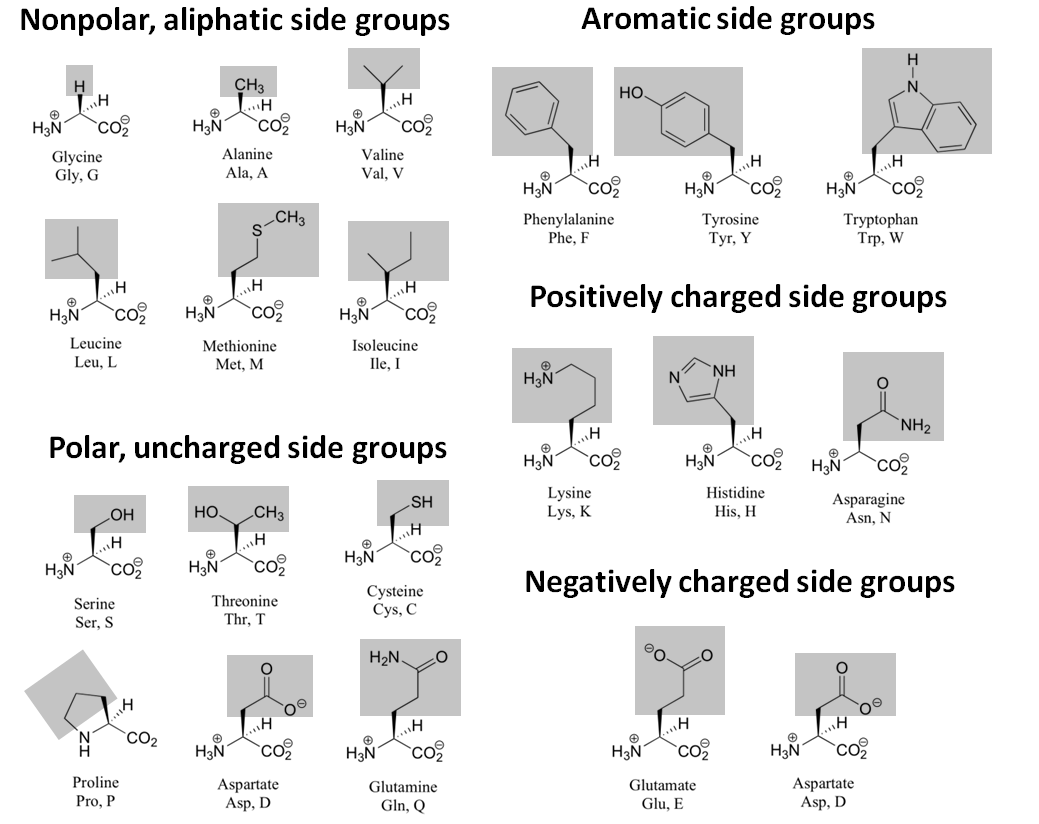
\includegraphics[width=0.8\textwidth]{Amino_Acids.png} \label{Amino_Acids}
\caption{20 Canonical Amino Acids, all with L configuration}
\end{figure}

\subsection{Carbohydrates \& Lipids}
Carboyhydrates have an empirical formula \ce{(CH_2O)_n}. They also must have an \textit{aldehyde} or \textit{ketone} functional group and at least \textit{two} alcohol functional groups. If a carbohydrate contains an aldehyde, it is referred to as an \textbf{aldose}. If it contains a ketone, it is referred to as a \textbf{ketose}. 

\subsection{D- and L- Isomers}
In Fischer projections, we care about the chiral carbon that is most distant from the carbonyl carbon. This chiral carbon is referred to as the \textbf{reference carbon}. If the hydroxyl group attached to that reference carbon is to the right, the molecule is the \textbf{D isomer}. If the hydroxyl group is to the left, the molecule is the \textbf{L isomer}. Most of the naturally occurring sugars are found in their D form (while most of the naturally occurring amino acids are found in their L form).

\subsection{Monosaccharides, Oligosaccharides, and Polysaccharides}
Sugars with five or more carbon atoms in their backbone prefer to be in the cyclic form. The C-1 carbon is the carbonyl carbon, also called the \textbf{anomeric carbon}. Two diastereomers of cyclic monosaccharides are $\alpha$ and $\beta$. In the $\alpha$-anomer, the \ce{-OH} group at the anomeric carbon is on the \textit{opposite} side of the ring from the \ce{-CH_2OH} group that is attached to the reference carbon. In the $\beta$-anomer, the \ce{-OH} group at the anomeric carbon is on the \textit{same} side of the ring as the \ce{-CH_2OH} group that is attached to the reference carbon. An example of anomers is shown in Fig. \ref{anomers}. Notice that, depending on the starting sugar, formation of the cyclic ring creates either a \textit{hemiacetal} group or a \textit{hemiketal} group. 
\begin{figure}[h!]
\centering
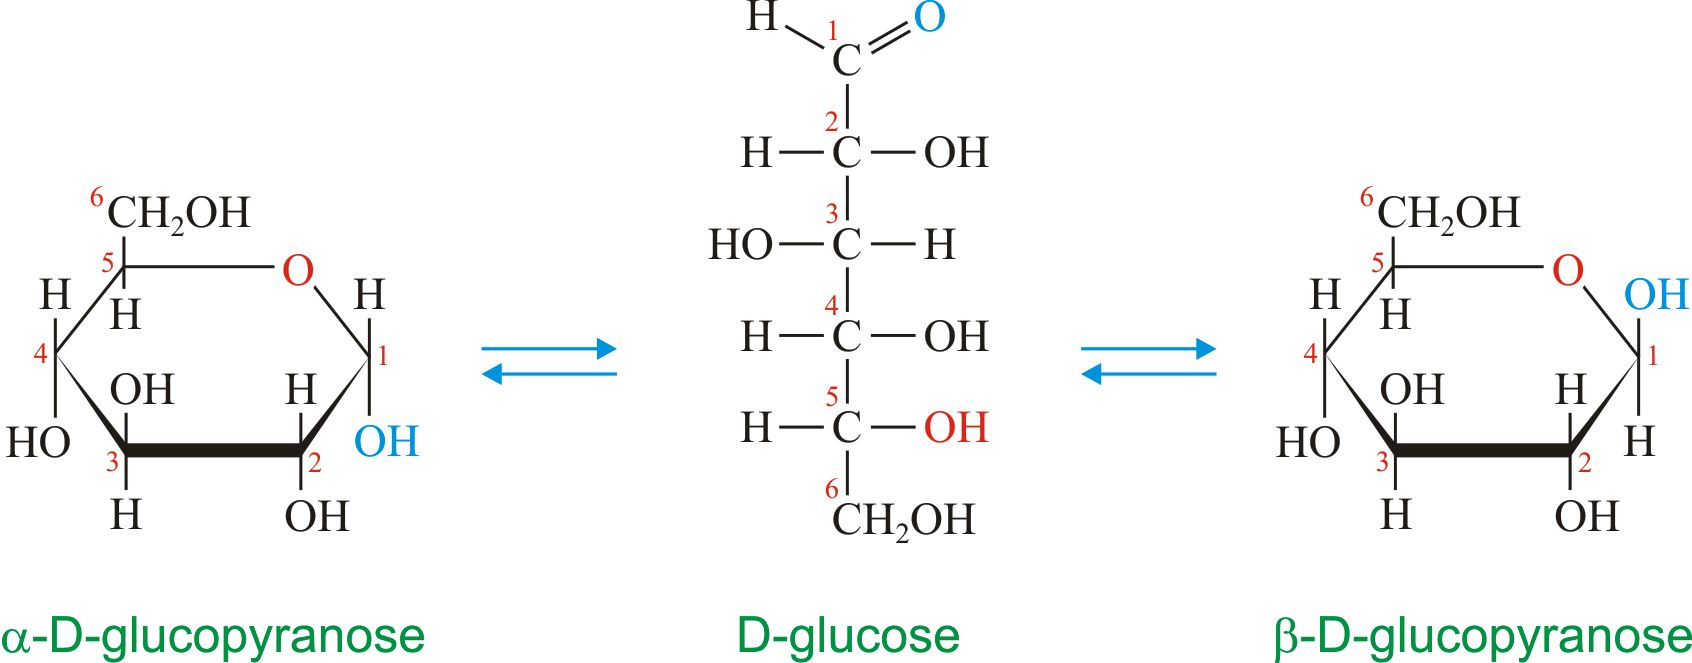
\includegraphics[width=0.8\textwidth]{anomers.png} \label{anomers}
\caption{Formation of the two anomers of D-Glucopyranose}
\end{figure}
\indent Two oxidizing agents used to identify the functional groups of carbohydrates are \textbf{Tollens' reagent} (which contains \ce{Ag^+}) and \textbf{Benedict's reagent} (which contains \ce{Cu^{2+}}). If an aldose or ketose is capable of reducing these ions, those sugars are referred to as \textit{reducing sugars}. Reducing sugars have the suffix \textbf{-ose}, while non-reducing sugars have the suffix \textbf{-ide}. Carbohydrates that contain a hemiacetal or a hemiketal group give positive tests with Tollens' and Benedict's reagents.\\
\indent A sugar is a non-reducing sugar if its hemiacetal or hemiketal group has been converted to an acetal or ketal group, respectively (i.e. through reacting with an alcohol). These non-reducing sugars will not react with either the Tollens' reagent or Benedict's reagent. \\
\indent The structure of lactose disaccharide has been given on the MCAT a number of times. Two important storage polysaccharids are \textit{starch} and \textit{glycogen}. Starch is a food reserve in plants. It is basically a bunch of D-glucose molecules linked together primarily with $\alpha\left(1\rightarrow 4\right)$ linkages, although there can be other types depending on the type of starch. Glycogen is the storage polysaccharide common to all animals, and is located primarily in skeletal muscle and liver tissue.

\subsection{Lipids}
Fatty acids are carboxylic acids with a hydrocarbon side chain. They can be either saturated or unsaturated. In nature, fatty acids are rarely free. Rather, they are esterified to a glycerol backbone to form a \textit{triacylglycerol}. There are a number of different types of lipids that we will discuss here:
\begin{enumerate}
	\item \textbf{Glycerophospholipids} (or phosphoglycerides) are the ones that we're most familiar with\textemdash two fatty acids esterified to the C-1 and C-2 carbons of glycerol, and a phosphate group attached to C-3. These molecules are amphiphilic, as they have nonpolar tails and a polar head.
	\item \textbf{Sphingolipids} do not have a glycerol backbone, and instead are derivatives of amino alcohols. The C-2 carbon has an amino group, and a fatty acid can be attached to it as well through an amide linkage\textemdash this molecule is called a \textit{ceramide}. Sphingomyelins are special types of sphingolipids that have a phosphoethanolamine or phosphocholine group attached to the C-1 carbon of the ceramide, and are abundant in the myelin sheaths that surround the axons of nerve cells.
	\item \textbf{Cholesterols} are synthesized in the cytosol. Steroids are based on cholesterols and synthesized in the mitochondria. Cholesterol is transported into the mitochondrion, and adrenocorticotropic hormone (ACTH) stimulates the conversion of cholesterol to pregnenolone. The five types of steroid classes are progesterone, glucocorticoids, mineralocorticoids, androgens, and estrogens.
\end{enumerate}
\noindent Cholesterol becomes pregnenolone, which then becomes progesterone. Progesterone can then either become testosterone, aldosterone, or cortisol. Testosterone can be further converted into estradiol. Progesterone is important for women to maintain pregnancy and the endometrial lining of the uterus, although it is also found in low levels in males. Cortisol (also known as hydrocortisone) is synthesized and secreted from cells in the cortex of the adrenal glands. In the liver, cortisol increases both glycogen synthesis and gluconeogenesis. In skeletal muscle, cortisol decreases glucose uptake and protein synthesis, and increases protein catabolism. In adipose tissue, cortisol increases lipid mobilization and decreases glucose uptake. Aldosterone is synthesized and released from cells in the adrenal cortex. It increases reabsorption of sodium ions in the kidneys, intestines, salivary glands, and sweat glands. This leads to retention of sodium in the extracellular fluid (ECF), thus increasing ECF volume, blood volume, blood pressure, and blood flow. Testosterone is important for sperm maturation in males and development of secondary sex characteristics. Estradiol is the primary estrogen in women and is important in the development of secondary sex characteristics and regulation of the ovarian cycle. \\
\indent Cholesterol decreases membrane fluidity at high temperatures and increases membrane fluidity at low temperatures. Basically, the way to remember this is that whatever the thermodynamically expected behavior of the cell fluidity is at a given temperature, cholesterol decreases the magnitude of that effect so that the membrane behavior never gets too extreme.\\
\indent In order to tolerate high temperatures, a thermophilic bacterium must have fatty acid tails that decrease the fluidity of its cell membrane. Saturated fatty acid tails have stronger Van der Waals interactions and thereby decrease the fluidity of cell membranes. Longer fatty acid tails have greater surface area for Van der Waals interactions, so they also decrease the fluidity of cell membranes. Therefore, long saturated hydrocarbon tails would best help the thermophilic bacteria have stable plasma membranes.\\
\indent Pinocytosis is the ingestion of liquid into a cell by the budding of small vesicles from the cell membrane.

\subsection{Cellular Reproduction and Chromosomes\textemdash Eukaryotic Cells}
\textbf{Chromatin} is a complex of dsDNA and histones (which are a type of protein). Histones are basic proteins consisting of a high percentage of Lys and Arg residues that bear of a positive charge. This allows them to easily establish a favorable electrostatic relationship with the negatively charged DNA polymers. There are also nonhistone proteins (i.e. RNA polymerase) that are acidic and bear a net negative charge. Chromatin condenses into \textbf{chromosomes} as the cell prepares for division. At metaphase, each chromosome consists of two \textbf{sister chromatids}, each held together through a constricted region called the \textbf{centromere}. \\
\indent There are five types of histones: H1, H2A, H2B, H3, and H4. A nucleosome is an association of these histones with a specific length of DNA. H2A, H2B, H3, and H4 are the \textbf{core} histones. The H1 histone is thought to play an important role in pulling the individual nucleosomes together to help with DNA condensation. 
\begin{figure}[h!]
\centering
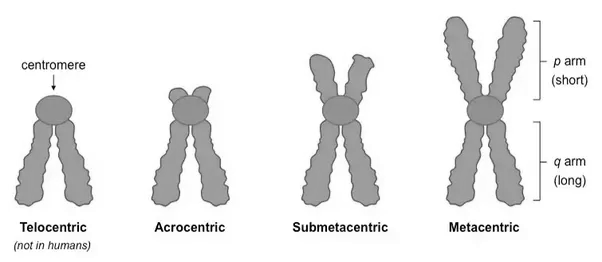
\includegraphics[width=0.65\textwidth]{chromosome_types.png} \label{chromosome_types}
\caption{General classification of eukaryotic chromosomes based on the position of the centromere.}
\end{figure}
Mitosis should honestly be pretty straightforward. The only thing is that for prophase, there may be some new terminology. At the beginning of prophase, the two \textbf{centriole} pairs begin to move apart, and microtubules begin to radiate from each pair in all directions, forming a star-like structure called an \textbf{aster}. The region from which the microtubules extend outward is called the \textbf{centrosome}, or MTOC (microtubule-organizing center). The microtubules ultimately form the \textbf{mitotic spindle}, and attach to the chromosomes at the \textbf{kinetochore}, a specialized area closely associated with the centromere.

\subsection{Meiosis}
Meiosis is technically composed of two processes\textemdash Meiosis I and Meiosis II\textemdash each of which s preceded by an interphase. During the second interphase immediately before meiosis II, the S period does not exist and so the DNA cannot be replicated again. Meiosis is a bit more complicated than mitosis, so let's take a look at it step by step:
\begin{itemize}
	\item Prophase I is longer and more complicated to prophase of mitosis, and can be divided into five stages: leptotene, zygotene, pachytene, diplotene, and diakinesis. During \textit{leptotene}, the replicated chromosomes have already started to condense and now become visible. During \textit{zygotene}, the synaptonemal complex forms where the maternal and paternal chromosomes come together to form the tetrads. This is in preparation for crossing over, although crossing over has not occurred yet. At this stage, there are 23 tetrads, 2 centromeres in each tetrad, and 46 chromosomes (based on the number of centromeres). During \textit{pachytene}, chromosomes continue to condense, and crossing over occurs. During \textit{diplotene}, the homologous chromosomes begin to separate and the events of crossing over become visible at structures called \textbf{chiasmata}. During \textit{diakinesis}, the nuclear envelope begins to break down, and the nucleoli disappear. 
	\item Metaphase I is unremarkable.
	\item During Anaphase I, the microtubules pull the homologous chromosomes apart, but the centromeres do \textit{not} divide. Each chromosome that migrates toward a pole is still composed of sister chromatids, and this pair is referred to as a \textbf{dyad}. Cytokinesis also begins at this step.
	\item Telophase I and Cytokinesis are unremarkable. After the completion of Meiosis I, we find that a diploid cell with 46 chromosomes has divided into two haploid cells, each with 23 chromosomes. This is therefore a \textbf{reductive division}.
	\item Interphase II is usually pretty brief.
	\item Meiosis II is pretty unremarkable. One thing to note is that the cells entering Meiosis II are already haploids. Also, because of the crossing over events from Meiosis I, the chromatids of each chromosome that are separating during Anaphase II can't actually be referred to as \textit{sister} chromatids because their DNA is no longer the same because of the genetic recombination.
\end{itemize}
\noindent Yeast are an example of a eukaryote that reproduces asexually.

\subsection{Biomembranes and Membrane Transport}
In lipid bilayers, recall that lateral diffusion of neighboring phospholipids is very common, but transverse diffusion (flip-flop) of phospholipids from one lipid plane to the next is a very rare event. Addition of cholesterol to a membrane acts to decrease fluidity, as the planar steroid ring inserts between neighboring fatty acid side chains and interferes with the movement of those chains. It might be a good idea to review that one problem about the symports and antiports from the Bi9 Final. \\
\indent There's also something called \textbf{group translocation} found in certain bacteria, where a sugar residue like glucose is phosphorylated as it is being transported through the plasma membrane. This type of transport is coupled to cellular metabolism. There's also \textbf{bulk transport} that involves \textit{indosomes} and \textit{endocytotic vesicles}. Many animal cells will show an invagination of a portion of their plasma membrane that will eventually pinch off to form an internalized vesicle. Bulk transport is where words like endocytosis, pinocytosis, phagocytosis, and exocytosis come in.

\subsection{Nucleus, Nucleolus, \& Ribosomes}
The nucleus is double membrane-bound. The outer membrane is actually considered to become part of the rough endoplasmic reticulum (RER). Between the inner and outer membrane is the \textbf{perinuclear space}. DNA replication and transcription occur in the nucleus, while translation happens outside in the cytosol. The diameter of \textbf{nuclear pores} is 10-20 nm. \\
\indent Within the nucleus is a highly organized region called the \textbf{nucleolus}. The nucleolus is \textit{not} a membrane-bound organelle. It is centered around certain chromosomes that contain \textit{nucleolus organizer regions}, and is involved in the synthesis of rRNA. If a cell is quite actively involved in protein synthesis (meaning that it needs a lot of rRNA), one would expect the nucleolus to be larger than if a cell were not as actively involved in protein synthesis. \\
\indent Eukaryotic ribosomes are composed to two subunits, each differing in size and content of RNA and protein. We talk about ribosome size based on a sedimentation coefficient called the \textbf{Svedberg unit (S)}, where one S $=10^{-13}$ sec. The rate at which a molecule sediments in an ultracentrifuge tells us something about its mass. The sedimentation coefficient of a complete eukaryotic ribosome is expressed as \textbf{80S}. Eukaryotic ribosomes have two subunits\textemdash a large subunit (60S) and a small subunit (40S). Note that 60S + 40S $\neq$ 100S; in other words, the values are not additive. Sedimentation coefficients are not linearly related to molecular weight, as they depend on the size and the shape of the molecule. \\
\indent The overall dimensions of a complete ribosome is about $\text{\textbf{20 nm}}\times\text{\textbf{30 nm}}$, and contains roughly 60\% rRNA and 40\% protein. The small subunit is about 9 nm in diameter and contains roughly half rRNA and half protein. The large subunit is roughly 25 nm in diameter and contains about 65\% rRNA and 35\% protein. \\
\indent Ribosomes are also found in the matrix of the mitochondria. Ribosomes found in the mitochondrial matrix differn in RNA and protein content, and are also smaller and sediment at about \textbf{55S}. Prokaryotic ribosomes are about \textbf{70S}. 

\subsection{Endoplasmic Reticulum, Golgi Apparatus, \& Lysosomes}
The ER is the largest membrane system in a eukaryotic cell. The \textbf{Smooth Endoplasmic Reticulum (SER)} is tubular in shape and is involved in the synthesis of a majority of the cell's membrane lipids (i.e. neutral fats, phospholipids, prostaglandins, and steroid hormones). Especially in hepatocytes (liver cells), the SER is involved in hydroxylation reactions that aid in the detoxification of drugs by making them more water soluble. The SER can also help catabolize liver glycogen in hepatocytes.\\
\indent The \textbf{Rough Endoplasmic Reticulum (RER)} is flat and sheet-like, and ribosomes on the cytoplasmic fact of the RER are bound to the membrane by their large (60S) subunit. Post-translational modification of proteins occur in the ER lumen, where certain amino acids are modified by hydroxylation and glycosylation events. \\
\indent For the Golgi Apparatus, the \textbf{cis} cisterna face the nucleus/ER, while the \textbf{trans} cisterna face the plasma membrane. The \textbf{medial} cisterna are located between the cis and trans cisternae. After a protein enters the cis cisterna and before it leaves the trans cisterna, it can be modified in a variety of different ways, including glycosylation, sulfation, and proteolysis.\\
\indent Lysosomes contain special enzymes that function at acidic pH values, and are referred to as \textbf{acid hydrolases}, which catalyze the general reaction \ce{A-B + H_2O -> A-H + B-OH}. There are some common acid hydrolases that you should know:
\begin{table}[h!]
\begin{tabular}{llll}
\hline
\textbf{Enzyme} & \textbf{Substrate} & \textbf{Bond Hydrolyzed} & \textbf{Example} \\
\hline
Proteases & Peptides & Peptide & Pepsidase\\
Glycosidase & Glycolipids & Glycoside & $\beta$-hexosaminidase\\
Lipase & Phospholipids  & Carboxylic Ester & Phospholipase\\
Nuclease & DNA & Phosphoric Diester & Acid Deoxyribonuclease\\
Phosphatases & Phosphomonoesters & Phosphoric Monoester & Acid Phosphatase\\
\hline      
\end{tabular}
\end{table}
\noindent Lysosomal enzymes are inactive at neutral pH. The hydrolysis products simply diffuse out of the organelle and are utilized in a variety of metabolic processes. We know that if this were not the case, the increasing solute concentration in the lysosome would eventually result in the lysis of the lysosome due to osmotic water entry into the lysosome, but this is not observed. \\
\indent Peroxisomes are membrane-bound organelles that have a number of enzymes, the most notable being \textit{catalase} that catalyzes the degradation of hydrogen peroxide \ce{H_2O_2}.

\subsection{Signal Hypothesis}
The Signal Hypothesis was covered in Bi9, and is import for co-translational transport. Many proteins have a signal sequence that binds to a signal recognition particle (SRP) in the cytoplasm, halting translation. The SRP chaperones the complex to the signal sequence receptor embedded in the membrane of the RER, and the signal sequence is cleaved by signal pepsidase. Translation then continues and at the same time, the polypeptide chain is transported into the ER lumen via Sec61. 

\subsection{Cytoskeleton}
\textbf{Microtubules} are composed of 13 protofilaments and are about 25 nm in diameter. Each protofilament has alternating $\alpha$-tubulin and $\beta$-tubulin proteins. The growth of microtubules occurs from \textbf{microtubule organizing centers (MTOCs)}. Three common centers are the centrosome (cell center), kinetochores (spindle attachment sites on chromosomes), and centrioles. Polymerization preferentially occurs at the (+) end.\\
\indent \textbf{Microfilaments} (actin filaments) are about 7 nm in diameter. Polymerization preferentially occurs at the (+) end. We have G-actin (globular) monomers, and F-actin (filamentous) polymerized subunits. \\
\indent \textbf{Intermediate filaments} are about 8 to 12 nm in diameter and differ in composition. For example, the intermediate filaments in epithelial cells are composed of keratins, while in muscle cells they are composed of desmin. 

\subsection{Prokaryotic Cells}
The two most frequently encountered bacteria are the \textbf{cocci} and the \textbf{rods}. Cocci are essentially spherical in shape while rods generally resemble the shape of a tube. Bacteria that have a rigid twist to their rod-like structure are called \textbf{spirilla}. If their twisted structure is more flexible, they are called \textbf{spirochetes}. Invaginations of bacterial cell membranes are called \textbf{mesosomes} with currently unknown function. \\
\indent Instead of membrane-bound organelles, prokaryotes often have structures called \textbf{inclusion bodies}, which can contain organic molecules like glycogen or inorganic molecules like phosphate granules. Prokaryotic ribosomes are \textbf{70S}, and are composed of a large \textbf{50S} subunit and a small \textbf{30S} subunit.\\
\textbf{Gram positive} bacteria have a rather thick, homogeneous \textbf{peptidoglycan} layer (20 nm to 80 nm) just outside their plasma membrane. \textbf{Gram negative} bacteria have a much thinner peptidoglycan layer (1 nm to 3 nm), in addition to an outer membrane that contains \textbf{lipopolysaccarides} and \textbf{porins}. The polysaccharide helps to stabilize the membrane, and also acts as an \textit{endotoxin} and provides a defense mechanism for the cell. \\
\indent Genetic material can be passed from one bacterial cell to the next by binary fission, bacterial conjugation, transformation, or transduction. Binary fission is basically asexual reproduction where one cell splits into two. In bacterial conjugation, genetic information is transferred by cell-cell contact. Donor strains of bacteria are $F^+$ (male), while the recipient bacteria are $F^-$ (female). The "$F$" refers to the \textbf{fertility plasmid}. Transformation is the uptake of genetic material from the surrounding medium. Transduction is the transfer of bacterial genes by viruses.

\subsection{Viruses}
The architecture of a virus is usually based on one of two structural motifs: \textbf{isometric} (usually in the form of an icosahedron) and \textbf{helical}. The viral protein coat is formed from \textbf{capsomers}. If there is no nucleic acid within the protein coat/shell, then the empty shell is referred to as a \textbf{capsid}. However, if there is nucleic acid within the protein shell, the complex is called a \textbf{nucleocapsid}.\\
\indent The genetic information within the genome of a virus may be encoded in either the language of DNA or RNA, and can be linear or circular, single- or double- stranded, and even segmented. However, no matter how the genetic information is stored in the virus, the translational process uses mRNA as a template. Therefore, by convention, we define that mRNA as being a \textbf{positive (+) strand} nucleic acid.\\
\indent Naked (non-enveloped) viruses gain access to the host's cytoplasm only by receptor-mediated endocytosis. The receptors on the cell surface of the host are usually located near specialized depressions called \textbf{\textit{clathrin-coated pits}}. Enveloped viruses can either enter through receptor-mediated endocytosis or by direct fusion with the plasma membrane. Release of viruses (whether naked or not) is mediated by pH changes, as the pH becomes more acidic in the endosome. 

\subsection{Metabolic Components\textemdash Enzyme Kinetics}
The \textbf{Michaelis-Menten Equation} describes the rate of a reaction as a function of the substrate concentration, assuming that the concentration of the intermediates is in steady state (meaning that the rate of change of the intermediates is zero or negligible). The equation is 
\begin{equation}
\begin{split}
V=\frac{V_{max}\left[S\right]}{\left[S\right]+K_M}
\end{split}
\end{equation}
\noindent where $K_M$ is the Michaelis constant. Notice that when $\left[S\right]=K_M$, then $V=V_{max}/2$, so this means that $K_M$ is equal to the substrate concentration at which the reaction rate is half of its maximal value. In general, a \textit{high} $K_M$ value indicates a \textit{weak} binding of the enzyme-substrate complex, while a \textit{low} $K_M$ value indicates a \textit{strong} binding of the enzyme-substrate complex. \\
\indent The \textbf{Lineweaver-Burk} Plot is basically the reciprocal of the Michaelis-Menten equation, and has the form of a straight line:
\begin{equation}
\begin{split}
\frac{1}{V}=\frac{K_M}{V_{max}}\frac{1}{\left[S\right]}+\frac{1}{V_{max}}
\end{split}
\end{equation}
\noindent When an enzyme is completely saturated with substrate, then the number of substrate molecules which are converted to product per unit time is referred to as the \textbf{turnover number}.\\
\indent There are two major types of enzyme inhibition: reversible and irreversible inhibition. There are two types of reversible inhibition: competitive and non-competitive inhibition. Allosteric inhibition is a subset of non-competitive inhibition. \\
\indent Competitive inhibitors decrease the rate of catalysis of the enzyme, and can be overcome at high concentrations of substrate. Initially, we have a lower $V_{max}$ for a given substrate concentration, but as we approach an infinite substrate concentration, the concentration of the competitive inhibitor becomes negligible and the enzyme catalyzed reaction will approach the same $V_{max}$ as before. When a competitive inhibitor is present, it changes the \textit{apparent} $K_M$ of the enzyme. The word `apparent' is used because each enzyme has a characteristic $K_M$ value for a given substrate. In other words, the $K_M$ of a competitively inhibited enzyme \textit{appears} to shift to a higher value, but if we add enough substrate, we will eventually reach the same $V_{max}$. On a Lineweaver-Burk plot, the $y-$intercept remains the same but the slope increases due to the competitive inhibitor.\\
\indent Non-competitive inhibition \textit{cannot} be overcome by increasing the substrate concentration. This means that we will have a \textbf{lower} apparent $V_{max}$ for the reaction. However, the $K_M$ will not change. On the Lineweaver-Burk plot, this looks like the $x$-intercept stays the same but the slope increases due to the non-competitive inhibitor, due to the decreased $V_{max}$. 

\subsection{Metabolic Components\textemdash Enzyme Mechanisms}
There are four classic enzymes in biochemistry:
\begin{enumerate}
	\item \textbf{Lysozymes} hydrolyze a specific glycosidic bond in the polysaccharide component of certain bacterial cell walls.
	\item \textbf{Ribonuclease} hydrolyzes the phosphodiester bonds in RNA polymers.
	\item \textbf{Carboxypeptidase} is a \ce{Zn}-containing digestive enzyme secreted by the exocrine cells of the pancrease, and hydrolyzes the carboxyl terminal peptide bond of protein polypeptide chains.
	\item \textbf{Chymotrypsin} hydrolyzes of either ester or peptide bonds. If a peptide is hydrolyzed, the products will be an amine and an acid. If an ester is hydrolyzed, the resulting products will be an alcohol and an acid. 
\end{enumerate}�

\subsection{Genetic Information\textemdash Classical Genetics}
Mendel's First Law of Heredity (also called the \textbf{Law of Segregation}) is that alternative alleles segregate from each other in heterozygous individuals and retain their identity. Mendel's Second Law of Heredity (also called the \textbf{Law of Independent Assortment}) is that the hereditary factors (i.e. genes) for different things assort independently of one another. Note that independent assortment of the genes will occur if they are located on different chromosomes or are far apart on the same chromosome.

\subsection{Genetic Loci \& Alleles}
\textbf{Tryptophan} is considered an \textbf{essential amino acid} because it is an amino acid that an organism cannot synthesize itself, and therefore must be obtained from the diet. An \textit{auxotroph} is a mutant that will grow only when its medium is supplemented with a particular compound which is not required by the normal wild type organism. The wild type organism is referred to as a \textit{prototroph}. By definition, an auxotroph will not grow on a minimal medium, while a prototroph will. \\
\indent \textbf{Pleiotropy} is when an individual allele has more than one effect on the phenotype (i.e. there's a mouse gene that determines both the fur coat color and the viability of the mouse). \textbf{Epistasis} is when multiple genes all contribute to a particular phenotype and are able to interact with one another. This occurs between different pairs of genes, \textit{not} between two members of an allelic pair. For example, in order for tryptophan to be synthesized, the dominant allele of all the genes involved in this biosynthetic pathway must be present (in the absence of tryptophan), so the genes involved in the biosynthetic pathway of tryptophan are said to act in an epistatic fashion.\\
\indent The short arm of a chromosome is called the $p$ arm, while the long arm of a chromosome is called the $q$ arm. 

\subsection{Pedigrees \& DNA}
In pedigree charts, males are squares and females are circles. If a square or a circle is filled in with a dark color, then that individual is affected with a given defect. If there is only one copy of any chromosome (i.e. \textbf{monosomy}), the individual will not survive development. The most common form of \textbf{trisomy} is for chromosome 21, which leads to Down's syndrome. It is an example of \textbf{aneuploidy} (the condition in which nuclei have an unbalanced set of chromosomes\textemdash that is, they do not contain an exact multiple of the haploid number of chromosomes). \\
\indent Double stranded DNA has a lower absorbance (by about 40 to 50\%) than single stranded DNA. Also, GC-rich DNA has a lower absorbance than AT-rich DNA at a given temperature. DNA replication is \textbf{semiconservative}. Adenine and guanine are purines (two rings in their structures), while thymine and cytosine are pyrimidines (one ring in their structures). Double stranded DNA is a right-handed helix.

\subsection{DNA Synthesis}
All of the dNTPs have a deoxyribose sugar backbone ($\beta$-D-2'-Deoxyribose) with an N-glycosidic linkage from the C-1 carbon to the purine or pyrimidine. There's also a phophomonoester linkage from the phosphate group to C-4 carbon of the sugar backbone, and additional phosphate groups can chain together via acid anhydride linkages. All dNTPs have 3 phosphate groups chained together. \textbf{DNA polymerase I} adds about 20 dNTP residues to the 3'-hydroxyl function of a pre-existing DNA strand. The dNTPS are added to the newly synthesized DNA chain in the $5'\rightarrow3'$ direction, which means the DNA template is read in the $3'\rightarrow5'$ direction. \\
\indent There are a couple different types of DNA structures that are helices: A-DNA, B-DNA, and Z-DNA. These aren't really important, just know that the canonical DNA form that we're all familiar with is the \textbf{B-DNA} with the major and minor grooves. In A-DNA, $\beta$-D-2-Deoxyribofuranose ring can pucker, and the minor groove essentially vanishes due to the puckering of the furanose ring. The type of helix that is found in A-DNA is also found in regions of double stranded RNA (e.g. involving hairpins) and in RNA-DNA hybrids. Z-DNA is actually a left-handed helix, and involves the phosphates in the backbone zigzagging due to a repeating dinucleotide unit, as opposed to a mononucleotide unit. In Z-DNA, when the pyrimidine bases and the ribose units are far apart, it is in an \textbf{anti} conformation, while it is in a \textbf{syn} conformation when the purine bases and the ribose units are close together.\\
\indent Positive supercoiling is twisting a DNA molecule around its own axis in the right-handed direction, while negative supercoiling is twisting a DNA molecule around its own axis in the left-handed direction (these conventions are for right-handed DNA). The number of times that one DNA strand can be wound around another DNA strand is referred to as its \textbf{linking number (L)}. \textbf{Topoisomers} are DNA molecules that differ only in their linking number. The degree of the linking number in DNA can be altered by enzymes called \textbf{topoisomerases}. \textbf{Type I} topoisomerases reversibly cleave \textit{one strand of DNA} and relaxes negatively supercoiled DNA, while \textbf{Type II} topoisomerases (e.g. DNA gyrase) reversibly cleaves \textit{both strands of DNA} and adds negative supercoils. Negatively supercoiled DNA prepares the DnA duplex for processes like replication, recombination, and transcription where the separation fo the two helical strands is required. \\
\indent The DNA replication process is very systematic. The synthesis of new daughter DNA is coupled to the unwinding of parental DNA at sites called \textbf{replication forks}, which occur at sites referred to as \textbf{origins} (ori for short). In order for the DNA double helix to unwind, \textbf{DNA gyrase} adds negative supercoils ahead of the advancing replication fork, as when the replication fork is initially unwound, positive supercoils are introduced making DNA separation rather difficult without the DNA gyrase activity. \textbf{Helicase} then binds to the ori site and catalyzes the ATP-driven unwinding of the duplex DNA. Single-stranded binding proteins then stabilize the unwound portion of the parental DNA. \\
\indent From here, both strands can serve as template strands, but DNA Polymerase I can only synthesize DNA in the $5'\rightarrow3'$ direction. We therefore have a leading strand with continuous replication, and also a lagging strand that uses \textbf{Okazaki fragments} to discontinuously synthesize the complementary strand (the primers used are RNA primers). DNA Polymerase III holoenzyme is used to synthesize the lagging strand (as opposed to DNA Polymerase I) because it is quicker and can add more dNTP's to the growing DNA strand. DNA polymerase I also has $5'\rightarrow3'$ exonuclease activity that allows it to remove the short segments of RNA primer, and then add deoxyribonucleotides to the free $3'$-hydroxyl function of the chain undergoing elongation. \textbf{DNA ligase} then joins together the Okazaki fragments. It is important to remember that replication of DNA can be bidirectional.



\end{document}